\documentclass[11pt]{article}
\usepackage[T1]{fontenc}
\usepackage{amsmath,amssymb,amsthm,mathtools}
\IfFileExists{lmodern.sty}{\usepackage{lmodern}}{}
\usepackage[margin=1in]{geometry}
\usepackage{array,longtable}
\usepackage{enumitem,booktabs,graphicx,tikz,placeins}
\usepackage[protrusion=false,expansion=false]{microtype}
\setlength{\emergencystretch}{1.5em}
\usetikzlibrary{arrows.meta,positioning,calc}
\usepackage[colorlinks=true,linkcolor=blue,citecolor=blue,urlcolor=blue]{hyperref}
% The title of the paper lives here and nowhere else.
% To change it: edit \papertitle (and \papersubtitle, which may be left empty), then run
%     python tools/sync_title.py            (copies the title into README.md, verification/README.md,
%                                            CITATION.cff and .zenodo.json)
%     python tools/sync_title.py --github   (also sets the GitHub repository description)
%     python paper/build.py                 (the PDF title page and the PDF metadata read this file)
% Write the title in plain text; TeX dashes (-- and ---) are converted by the script.
\newcommand{\papertitle}{The thermodynamics of deadlines: one law for the work cost of acting in time}
\def\papersubtitle{}

\hypersetup{pdftitle={\papertitle},pdfauthor={Seth Douglas and Nidhal Mghirbi}}

\numberwithin{equation}{section}
\newtheorem{theorem}{Theorem}[section]
\newtheorem{proposition}[theorem]{Proposition}
\newtheorem{lemma}[theorem]{Lemma}
\newtheorem{corollary}[theorem]{Corollary}
\theoremstyle{definition}
\newtheorem{definition}[theorem]{Definition}
\theoremstyle{remark}
\newtheorem{remark}[theorem]{Remark}

\newcommand{\Tr}{\operatorname{Tr}}
\newcommand{\kB}{k_{\mathrm B}}
\newcommand{\Trt}{\kappa_\beta}
\newcommand{\Tcap}{\mathcal T}
\newcommand{\Pp}{\mathcal P}
\newcommand{\Pt}{\widetilde{\mathcal P}}
\newcommand{\Kb}{K_\beta}
\newcommand{\Dil}{\mathcal C}
\providecommand{\tr}{\operatorname{tr}}
\providecommand{\R}{\mathcal R}
\providecommand{\G}{\mathcal G}
\providecommand{\K}{\mathcal K}
\providecommand{\eps}{\varepsilon}
\providecommand{\id}{\operatorname{id}}
\newcommand{\PROV}[1]{}
\providecommand{\supp}{\operatorname{supp}}
\providecommand{\Span}{\operatorname{span}}
\providecommand{\osc}{\operatorname{osc}}
\providecommand{\h}{h_2}
\providecommand{\T}{\tfrac12\|\cdot\|_1}
\providecommand{\D}{D_{\mathrm{nat}}}

\title{\textbf{\papertitle}\ifx\papersubtitle\empty\else\\[6pt]\large\papersubtitle\fi}
\author{Seth Douglas \and Nidhal Mghirbi}
\date{October 2026 \\[2pt] {\small Version 1.0.0}}

\ifdefined\pdftrailerid\pdftrailerid{}\fi
\begin{document}
\maketitle

\begin{abstract}
A quantum channel says what happens to each input, not when inputs arrive, when outputs leave for good, or what must be handed back. We show that for every finite schedule in which each carrier returns with its Hamiltonian and the controller comes back, the optimal work per use at vanishing error is the least entropy one implementation must add to its own record, plus the energy it hands over, against the most demanding observer. Landauer's bound, the thermodynamic capacity of Faist, Berta and Brand\~ao in the time-covariant case, and the real-time costs of channels and processes are this law on different schedules. The cost survives arbitrarily slow operation: order, not speed, sets it. Releasing each output of a repeated memoryless channel before the next input arrives costs nothing extra for classical channels, a positive amount for partial reset at every temperature, and $k_{\mathrm B}T\ln3$ per use for the Werner--Holevo qutrit at zero Hamiltonian, which is essentially free in batch. For a classical task with zero Hamiltonians that releases a past and later answers a question about it, the real-time and held prices are logarithms of two fiber counts; for reversible questions they differ by the logarithm of the number of classes of pasts that later questions tell apart. With a returned clock, the batch cost of every channel is a single-letter quantity, equal to the capacity when the environment can carry the channel's energy change; otherwise the clock's spread must grow at least linearly with the number of uses. Freeness is decidable in batch for exact algebraic data and undecidable in real time, already in a fixed dimension. A two-qubit process that is free when held costs every early-release device at least $0.87\,k_{\mathrm B}T\ln2$ per episode at one percent error and budgets of $0.025\,k_{\mathrm B}T\ln2$; for a classical version we propose a three-arm feedback-trap protocol.
\end{abstract}

\noindent\emph{The authors developed this work with AI models from more than one developer and take responsibility for every claim. The whole paper has been reviewed nine times by a model from a developer other than that of the models that helped write it, and the fixes from those reviews, and from a review of the experimental design, are applied. How the work was done, and what the machine checks cover, is described at the end of the paper.}

\setcounter{tocdepth}{1}
{\small\tableofcontents}

\section{Introduction}\label{sec:intro}

Landauer's principle says that resetting an unbiased bit, stored in two states of equal energy, costs at least $\kB T\ln2$ of work~\cite{Landauer61}. For $n$ uses of a quantum channel, Faist, Berta and Brand\~ao found the least work per use, the thermodynamic capacity, when the device may collect all of its inputs before it releases any output~\cite{FBB19,FBB21}: to leading order in $n$, for every channel when Gibbs-preserving maps are free, and for time-covariant channels with thermal operations. Both results describe what a device does to its inputs. Neither says when the device may touch what, and that turns out to be half of the price.

Here is the smallest case. Two bits $a$ and $b$ arrive in turn, and the device must return $a$ and then $a\oplus b$. If it may hold $a$ until $b$ arrives, one CNOT does the job and nothing is left behind. If $a$ must leave before $b$ arrives, the device must keep a copy of $a$, and once $a\oplus b$ has left too that copy is correlated only with carriers that are gone; erasing it costs $\kB T\ln2$ at any speed (Figure~\ref{fig:three}). A third schedule shows that the cost is in the release, not in the early delivery: if the device copies $a$ into a blank register, lends $a$ to the observer, and gets it back unmodified before $a\oplus b$ is due, a second CNOT uncomputes the register and the cost is again zero. The map is the same in all three cases. What changes is what the device can still reach when it has to clean up.

\begin{figure}[t]
\centering
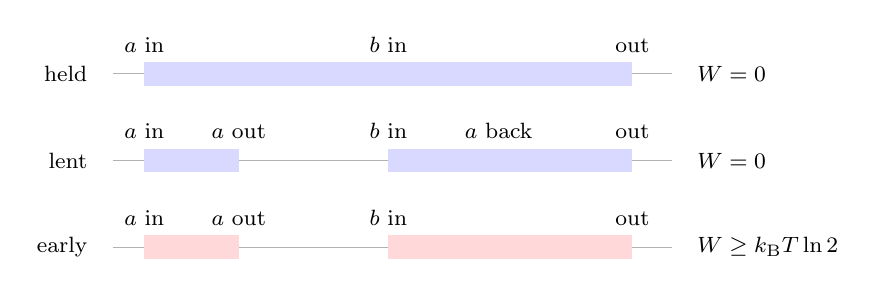
\begin{tikzpicture}[x=1cm,y=1cm,font=\footnotesize]
  \foreach \row/\y/\lab/\w in {0/2.2/held/{$W=0$}, 1/1.1/lent/{$W=0$}, 2/0/early/{$W\ge\kB T\ln 2$}} {
    \node[anchor=east] at (-0.2,\y) {\lab};
    \node[anchor=west] at (7.3,\y) {\w};
    \draw[gray!60] (0,\y) -- (7.1,\y);
  }
  % held
  \fill[blue!15] (0.4,2.05) rectangle (6.6,2.35);
  \node[above] at (0.4,2.35) {$a$ in}; \node[above] at (3.5,2.35) {$b$ in}; \node[above] at (6.6,2.35) {out};
  % lent
  \fill[blue!15] (0.4,0.95) rectangle (1.6,1.25); \fill[blue!15] (3.5,0.95) rectangle (6.6,1.25);
  \node[above] at (0.4,1.25) {$a$ in}; \node[above] at (1.6,1.25) {$a$ out}; \node[above] at (3.5,1.25) {$b$ in}; \node[above] at (4.9,1.25) {$a$ back}; \node[above] at (6.6,1.25) {out};
  % early
  \fill[red!15] (0.4,-0.15) rectangle (1.6,0.15); \fill[red!15] (3.5,-0.15) rectangle (6.6,0.15);
  \node[above] at (0.4,0.15) {$a$ in}; \node[above] at (1.6,0.15) {$a$ out}; \node[above] at (3.5,0.15) {$b$ in}; \node[above] at (6.6,0.15) {out};
\end{tikzpicture}
\caption{The same task, the same slowness, three schedules. Return $a$, then return $a\oplus b$; shaded bars show when the device can act on its carriers. Holding $a$ until $b$ arrives allows reversible cleanup, and so does lending it, provided the observer returns it unmodified before cleanup. Releasing $a$ for good strands a copy of it in the device, and the copy must be paid for. Appendix~\ref{app:classes} proves the general form: for reversible questions, the order price of a released past is the logarithm of the number of classes of pasts that later questions tell apart.}
\label{fig:three}
\end{figure}

Finite-time thermodynamics charges for speed: for protocols with a reversible quasistatic limit, the excess work due to finite speed vanishes as the protocol is slowed~\cite{SalamonBerry83,Crooks07,Proesmans20}. The charge above survives that limit. All rates in this paper allow devices of any size and any running time. Thermodynamics therefore charges for time twice: once for speed, which patience removes, and once for order, which it does not. The resource is not elapsed time. It is the capability that must remain available after access to an earlier output has been irreversibly surrendered. For classical information engines, costs that survive slow operation because processing goes step by step are known: the modularity dissipation of information ratchets~\cite{BMC18}, which Loomis and Crutchfield trace to temporal locality~\cite{LoomisCrutchfield20}, the dependence of dissipation on the input distribution a device was built for~\cite{KolchinskyWolpert17}, and the online cost of agents~\cite{Thompson25}. Those costs are forced on every implementation of a given architecture: a modular or temporally local design, a device tuned to one input distribution, an agent whose memory is a function of its past. Here the price is forced by the release schedule on every implementation, whatever its memory, and for memoryless channels it is purely quantum.

\begin{table}[tbp]
\centering
\small
\begin{tabular}{@{}>{\raggedright\arraybackslash}p{3.1cm}>{\raggedright\arraybackslash}p{10.0cm}>{\raggedright\arraybackslash}p{2.5cm}@{}}
\toprule
Result & Statement & Where\\
\midrule
One law for every schedule & For schedules whose observer-owned carriers return with their Hamiltonians, the optimal deterministic work rate is $\kB T\ln2\,K_\beta^S$, the least record entropy plus handed-over energy against the hardest observer. Lower bound: a one-page identity. Upper bound: a coherent recorder and a positive heat correction. & Theorem~\ref{to:thm:law}, Section~\ref{to:sec:law}, Appendix~\ref{app:law}\\
Only quantum channels pay for releasing & For repeated uses of one memoryless channel, each output released before the next input arrives, the real-time rate adds to the capacity's integrand, input by input, the least output--device correlation any dilation must leave, so the surcharge over the capacity is a difference of two maxima. The surcharge is zero for every classical channel; positive for partial reset at every temperature; $\kB T\ln3$ per use for Werner--Holevo, against essentially nothing in batch. Classical tasks with memory can still pay (Figure~\ref{fig:three}). & Theorems~\ref{thm:main-realtime}--\ref{thm:main-dichotomy}, Appendix~\ref{app:channels}\\
A clock has an exact price & With a returned clock, the batch cost of every channel is the single-letter quantity $B(\Phi)\ge$ capacity, with equality whenever $H-\Phi^*(H)\in\operatorname{span}\{A_i^*A_j\}$. When $H-\Phi^*(H)$ lies outside that span the channel's time orbit is Heisenberg-estimable and the clock must grow linearly; the Hadamard gate shows that $B(\Phi)$ can still equal the capacity there. & Theorem~\ref{to:thm:batchlaw}, Theorem~\ref{thm:main-heisenberg}, Appendix~\ref{app:batch}\\
What a released past must keep & Release $x$, then answer $y$ with $g(x,y)$: in real time the price is $\log_2$ of the largest fiber of $(\text{class of }x,y)\mapsto g$, when $x$ may be held it is the Landauer cost (the logarithm of the largest $y$-fiber, maximized over $x$ and the answer), and the difference, the order price, is $\log_2$ of the number of continuation classes (the causal states of the task) for reversible questions. A record is not yet a price: it can be passed into the answer. Linear tasks give a rank; deciding whether holding $m$ carriers lowers it is NP-complete. & Theorem~\ref{thm:classes}, Proposition~\ref{to:prop:rank}, Appendix~\ref{app:classes}\\
Holding is decidable, releasing is not & Batch freeness is decided by linear algebra for algebraic channel and Hamiltonian entries, when $\beta$ or the Gibbs state is algebraic. Real-time freeness of a generalized dephasing channel with cyclotomic entries is undecidable in a fixed dimension, and the free set is not recursively enumerable. & Theorem~\ref{thm:main-undecidable}, Appendix~\ref{app:channels}\\
A certificate and a protocol & A two-qubit process, free when held, costs every early-release device at least $[1-h_2(e)-e\log_23-P]\,\kB T\ln2$ per episode, where $P$ bounds the controller's and battery's budgets, which the Pauli measurements do not certify; $0.878$ at $e=1\%$ and $P=0.025$. A classical protocol with three arms, a graded control and record accounting is proposed as a design, in a feedback trap or, preferably, a preprogrammed physical memory; its record-export interface and controller bounds remain to be established. & Proposition~\ref{to:prop:certificate}, Section~\ref{sec:protocol}\\
Beyond thermodynamics & Order has a per-use price in entanglement and coherence theory as well; for the delayed-choice task one retained qubit is the common requirement, with no single exchange rate between theories. & Section~\ref{to:sec:beyond}\\
\bottomrule
\end{tabular}
\caption{Results at a glance. Entropies are in bits; $h_2$ is the binary entropy. Section~\ref{sec:contract} gives the contract and the results that depart from it.}
\label{tab:glance}
\end{table}

\paragraph{The principle.} A device is built before the observer chooses its inputs, and it must serve every observer the schedule admits. Its work rate is the least entropy that one implementation must add to its own record, plus the energy it hands over to the carriers, against the most demanding observer. Three things decide it. \emph{Access} decides which corrections remain possible: a device that still holds its outputs can erase its record using them as side information~\cite{delRio11}, as the batch construction of Faist, Berta and Brand\~ao does~\cite[Sec.~7]{FBB21}; a device that has released them cannot, and whatever its record shares with them is stranded. \emph{Universality} decides whether those corrections can belong to one device. Faist, Berta and Brand\~ao showed that in batch one device can serve every input at the cost of the hardest one~\cite{FBB19,FBB21}, and that a known i.i.d.\ input can even be served at its own free-energy cost with thermal operations and a sublinear source of coherence~\cite[Prop.~8.3]{FBB21}. With a clock that must return, one device can cost more than its hardest input (Section~\ref{to:sec:clock}). \emph{Return obligations} decide what may not be left behind as an unpaid change: a clock lent to the device must come back, and that requirement decides whether some channels can be run at all~\cite{MarvianSpekkens19,LostaglioMuller19} and, for others, what they cost.

\paragraph{Results at a glance.} Table~\ref{tab:glance} lists what the paper proves and where. Everything below is a consequence of one functional on one contract (Section~\ref{sec:contract}).

\paragraph{What the constructions are.} Every achievability statement in this paper is a statement about optimal rates. The devices that attain them are built for a number $n$ of uses known in advance, and they use clocks whose spread grows with the number of uses, startup capital that may grow without bound, and reservoirs with very large gaps; they show what is possible, not how to build an efficient or autonomous engine (Section~\ref{sec:discussion}). The lower bounds, by contrast, hold for every device at every size.

\paragraph{What is new.} The thermodynamic capacity, Landauer's bound, the side-information erasure of~\cite{delRio11}, the entropy accumulation of~\cite{DFR20} and the metrological results we invoke, the Kraus-span condition and its error-correcting code~\cite{ZhouJiang21} and their Markovian forms~\cite{ZhouZhangPreskillJiang18,DemkowiczCzajkowskiSekatski17}, are prior work, and so are the modularity and online costs of classical engines~\cite{BMC18,LoomisCrutchfield20,Thompson25} and the entanglement cost of simulating channel uses sequentially against adaptive testers~\cite{Wilde18}. Items (1)--(3) and (5) below, and the certificate of item (6), first appeared in four companion papers~\cite{Order,SaveWork,Answering,KeepingTime}, which a short letter summarizes~\cite{Letter}, and Appendix~\ref{app:companions} maps every statement taken from them. This paper consolidates those results and adds the fiber law of item (4) and the laboratory protocol of item (6). Apart from that companion work, to our knowledge the following are new.
\begin{enumerate}[label=(\arabic*),leftmargin=*,itemsep=1pt,topsep=2pt]
\item The schedule functional and the law of Theorem~\ref{to:thm:law}, with the recorder-and-dual construction that attains it for arbitrary interleavings, overlaps and loans.
\item The real-time law for channels in work units at every temperature, its strong converse at every fixed error for controllers that start thermal (a controller with a broad energy bank breaks it; whether it survives a controller whose capital has spread $o(n/\sqrt\eta)$, with $\eta$ its return error, is open; Remark~\ref{sw:rem:thermal-controller}), and the dichotomy of Theorem~\ref{thm:main-dichotomy}; at zero Hamiltonian, in units of purity, the rate and its zero set are in our earlier work~\cite{Memory,ImmediateDelivery,Douglas26closed}, with a strong converse at zero rate~\cite{Flagship}.
\item The batch law $B(\Phi)$ with a returned clock, its span criterion, and the identification of that criterion with the Hamiltonian-not-in-Kraus-span condition of Zhou and Jiang for the channel's time orbit.
\item The fiber law of Theorem~\ref{thm:classes}, which separates the order price of a released past from the Landauer cost of its answer. Its classes are the causal states of the task's $\varepsilon$-transducer~\cite{BarnettCrutchfield15}. Our tasks are in place, each answer overwriting its question, and that convention is what makes the released task of Figure~\ref{fig:three} cost $\kB T\ln2$. For classical causal agents that keep each question and write the answer to a fresh cell, Thompson et al.\ give the online cost for a given input process, which is zero for that task; their formula~\cite[Eq.~(3)]{Thompson25}, the information the memory stores about the last input and output minus what it holds about the next, is the averaged form of passing a record into an answer. New here is the worst case: neither the observers who might ask a distinguishing question nor an observer who steers the answer forces the price alone, the lower bound pairs them, and the result is the minimax price over every implementation, for devices with any memory required to serve every quantum observer with references, with an explicit small-error loss independent of the number of episodes and the private-device dimension.
\item The undecidability of real-time freeness in a fixed dimension, through the constant-sized correlation problem of Fu, Miller and Slofstra; in growing dimension, at zero Hamiltonian, it is in our earlier work~\cite{Flagship}.
\item The finite certificate of Proposition~\ref{to:prop:certificate}, and the protocol proposed in Section~\ref{sec:protocol}, built on the feedback-trap test of Landauer's principle~\cite{Jun14}. That access to a copy changes the cost of erasure is established~\cite{Bennett03,delRio11,Orlov12}, and the erasure of a fraction of a bit, the cleanup step of the graded control, has been measured in a feedback trap~\cite{Gavrilov17}. What the proposed protocol adds is a controlled release schedule with control arms, a graded helper control, and an explicit ledger of records and blank resources, whose readout interface and hardware budgets remain to be established.
\end{enumerate}

\paragraph{Reading guide.} Section~\ref{sec:contract} fixes the contract and says what it rules out. Section~\ref{to:sec:law} states the law and proves its lower bound in full. Sections~\ref{to:sec:table}--\ref{to:sec:clock} read the law on the schedules that matter most, Section~\ref{sec:classes} on tasks that release a past, and Section~\ref{to:sec:computability} on the complexity of freeness. Section~\ref{to:sec:measure} and Section~\ref{sec:protocol} are for experimenters. Section~\ref{sec:related} places the results among prior work, Section~\ref{sec:verification} says which statements are checked by machine, by formal proof and by text alone, Appendix~\ref{app:glossary} defines every term of art, and Appendix~\ref{app:companions} gives the number of every result in the companion papers. The appendices contain the proofs, complete except for two results imported from our earlier preprints, Lemma~\ref{sw:lem:smoothing} and~\cite[Thm.~3.2(a)]{Memory} (Section~\ref{sec:channel-statements}): Appendix~\ref{app:law} the law, Appendix~\ref{app:module} the physical module and the law for processes with memory, Appendix~\ref{app:channels} memoryless channels, Appendix~\ref{app:batch} the returned clock, Appendix~\ref{app:classes} continuation classes, and Appendices~\ref{to:app:release}--\ref{to:app:rank} the release lemma, the numbers of Section~\ref{to:sec:beyond}, the two-qubit certificate and release rank. A reader who wants only the mechanism can read Sections~\ref{sec:intro}--\ref{to:sec:law} and Appendix~\ref{app:classes}; a reader who wants only the experiment can read Sections~\ref{to:sec:measure}--\ref{sec:protocol}. The numbers quoted in Sections~\ref{to:sec:law}--\ref{to:sec:beyond} are recomputed, and the finite identities listed in Table~\ref{tab:verification} checked, by a deterministic verification package with negative controls (Section~\ref{sec:verification}).

\paragraph{Two layers.} The mechanism is not specific to heat; what thermodynamics adds is the form of the price and its complexity. The free energy relative to the Gibbs state splits across a release as
\begin{equation}\label{eq:split}
D(\rho_{CO}\|\gamma_C\otimes\gamma_O)=D(\rho_C\|\gamma_C)+D(\rho_O\|\gamma_O)+I(C{:}O),
\end{equation}
so at a fixed state the price of releasing $O$ from a device $C$ is a mutual information, the free energy of correlations that joint operations could have recovered~\cite{PerarnauLlobet15}. Optimized over inputs, the surcharge is a difference of two maxima rather than the largest mutual information, because the two maxima can sit at different inputs (Section~\ref{to:sec:waiting}). For classical computation this is the modularity dissipation of Boyd, Mandal and Crutchfield, the free energy of correlations lost to local control~\cite{BMC18}; here the cut is a release in time. And the set of channels that cost nothing in real time is undecidable, while its batch counterpart, and every analogue we know outside thermodynamics, is decidable.

\section{The contract, and what it rules out}\label{sec:contract}

Every work rate in this paper is an optimal asymptotic rate at vanishing error over a complete interaction, with hardware allowed to grow. Such a statement is only as good as the contract behind it, so we state the contract first, as a threat model: what the device is allowed, what the observer is allowed, and which loopholes the rules close. Appendix~\ref{app:glossary} defines each term in one line.

\paragraph{The device.} A device consists of a controller $C$, a mechanical battery $W$ and Gibbs reservoirs $R$ at inverse temperature $\beta$, all declared in advance and initially independent. The controller holds all hardware: memory, clocks, catalysts, routing registers, records and any workspace not charged to the battery. Every operation is a unitary that conserves the total energy of the systems it acts on. There is no external source of coherence and no Gibbs-preserving map supplied as a black box. Measurements and records are part of the dilation and are counted. Work is the battery's mean loss of energy, and the battery's entropy may change only by $o(n)$, so that it cannot hide a second bath. Work is \emph{deterministic} when the battery starts in an energy eigenstate, ends in a fixed level with probability tending to one, and its mean absolute energy deviation from that level is $o(n)$. The battery is \emph{stationary} if its initial state commutes with its Hamiltonian; a battery in a broad superposition of energy levels would itself be a clock, which the device could spend without returning it.

\paragraph{The observer.} The observer supplies the carriers and may choose them adaptively, using only outputs already released, its own memory and its quantum references; it may entangle inputs across visits and across blocks, keep purifications, and act on a loan before returning it. It cannot read the device's inert initial purifier. The error is the largest trace distance, over all such observers, between the final state of the observer's systems with the device and with the ideal target: the strategy distance of~\cite{Chiribella08,GutoskiWatrous07}. For batch operation this is the half diamond distance.

\paragraph{The schedule.} Definition~\ref{to:def:schedule} below makes the schedule a first-class object: a finite ordered list of arrivals and releases of carriers the observer owns, each returned with the Hamiltonian it arrived with. Batch, real time, delayed release, interactive processes and loans are schedules. Schedules that create or retire carriers, or change Hamiltonians, need an explicit inventory term or a physical switch, and Section~\ref{to:sec:law} says exactly what.

\paragraph{The return rule, and why it has the form it has.} The controller returns \emph{approximately}: uniformly over observers, its final joint state with everything else is close in trace distance to its initial state tensored with the rest, and its actual mean energy and its actual entropy each change by $o(n)$. Trace-distance closeness alone would not do. As Faist, Oppenheim and Renner warned, a catalyst returned only approximately can embezzle work~\cite{FOR15}. Here is the loophole in its simplest form: a reference register in a broad, flat superposition of $n^2$ energy levels, shifted down by $n$ levels, is within trace distance about $\sqrt{2/n}$ of itself yet has handed over $n$ quanta of energy. Refunding energy alone is not enough either: a large mixed register can stay within trace distance $\eta$ of its initial state after every use while absorbing $n$ bits of entropy, with about $n/\eta$ qubits~\cite{Mausberg26}, and a controller built that way is a second bath. The lower bound of Theorem~\ref{to:thm:law} sees the controller only through $\Delta E_C-\kB T\ln2\,\Delta S_C$, so we require each term to be $o(n)$. The contract allows the controller's \emph{startup capital}, its initial free energy, to be as large as one likes and to grow with $n$; capital is invested and must come back, and it is not part of the rate. A controller that comes back only in state, as an embezzling state does, can lower the battery's work to the capacity or below it, but only by paying the difference from its own free energy, like a second battery; this is quantified in Appendix~\ref{app:batch}.

\paragraph{What the contract does not cover.} Resources that start correlated with the controller and must be returned in a prescribed joint state are not covered: such a borrowed catalyst would have to be modelled jointly with the controller, and the product initial state used throughout would fail. Promises of product inputs, restrictions on loans and frozen external fuel would be additional contract data; the observer class here has none of them. A task may, however, restrict its admissible inputs by a promise that is part of the task, and so narrow the observer class: the task of Theorem~\ref{thm:classes} is one, and its bounds are proved directly in Appendix~\ref{app:classes}. The lent schedule of Figure~\ref{fig:three}, arm~(ii) of Section~\ref{sec:protocol}, instead needs a restriction on loans, that the observer return the carrier unmodified; Section~\ref{sec:protocol} states it as a contract of its own.

\paragraph{Units.} Entropies are in bits and work in units of $\kB T\ln2$ in the main text; Appendices~\ref{app:law} and~\ref{app:module} use nats where the proofs are shorter.

Table~\ref{to:tab:contract} collects the contract, and Table~\ref{tab:exceptions} the principal departures of the thermodynamic results from it; Section~\ref{to:sec:beyond} fixes its own free operations, currencies and output inventory.

\section{Schedules and the law}\label{to:sec:law}\label{sec:law}

Unless a result states an exception, the contract of Section~\ref{sec:contract} applies; Table~\ref{to:tab:contract} below collects it.

\begin{definition}[Schedule]\label{to:def:schedule}
A schedule $S$ is a finite, ordered list of arrival and release events. A visit $v$ brings a carrier $P_v$ with Hamiltonian $H_v$ into the device at its arrival and returns the same carrier, with the same Hamiltonian, at its release. Visits of the same carrier cannot overlap; visits of different carriers may overlap, and releases may come in any order. The device can act on a carrier only during its visit. A later loan of a carrier that the observer owns is a new visit, and its state may be correlated with everything the observer holds. The observer supplies the carriers and may choose them adaptively, using only outputs already released, its own memory and its quantum references; every receipt or message the observer sees is written on a carrier the observer has supplied, and its delivery is that carrier's release.
\end{definition}

Batch operation is the schedule in which every input arrives before any output is released; real time is the schedule in which input $t+1$ arrives only after output $t$ has left; a process with memory interleaves the two.

\begin{definition}[The schedule functional]\label{to:def:functional}
A \emph{private extension} of a target strategy $T$ on $S$ consists of an initial device state $\tau$, an inert purification $F$ of it that is never acted on, and unitaries on the device and the carriers present, following $S$, whose marginal strategy is within $\varepsilon$ of $T$ in the strategy distance, the largest trace distance over adaptive testers. These unitaries need not conserve energy; the extension is a mathematical object. For a purified tester $t$, an observer allowed by the schedule that keeps its initial purifying systems and everything it discards coherently, let $Z$ be everything it owns at the end, including these systems, its references and every released carrier, with no duplicate copy of a carrier loaned again; the tester starts independent of the device and of $F$. Let $E_t=\sum_v[\Tr H_v\rho_{v,\mathrm{release}}-\Tr H_v\rho_{v,\mathrm{arrival}}]$ be the energy handed over. Set
\[
k_{S,\varepsilon}(T)=\inf_{\text{private extensions}}\ \sup_{\text{purified }t}\Bigl[\tfrac{\ln2}\beta S(Z|F)_t+E_t\Bigr],
\]
and let $K_\beta^S(T)=\beta\,\bar k^S(T)/\ln2$, where $\bar k^S(T)=\inf_{\varepsilon_n\to0}\limsup_n k_{S_n,\varepsilon_n}(T_n)/n$ is the regularized rate along the block schedules $S_n$. As a check of the normalization, resetting a maximally mixed bit with zero Hamiltonian gives $k=\kB T\ln2$.
\end{definition}

Because the tester is purified and starts independent of the device, the final state of $F$, the device and $Z$ is pure, so $S(Z|F)=S(\omega)-S(\tau)$, with $\omega$ the device's final state, is the entropy the extension adds to its own record: the device cannot read $F$, and the same tester supplies both the entropy and the energy term. The purification is needed. For the identity channel on a qubit with zero Hamiltonian, run by a device that does nothing, a tester that feeds $I/2$ and keeps no purifier would be charged $S(Z|F)=1$ although the device adds no entropy; with the purifier in $Z$, $S(Z|F)=0$.

\begin{table}[tbp]
\centering
\small
\begin{tabular}{@{}>{\raggedright\arraybackslash}p{2.6cm}>{\raggedright\arraybackslash}p{12.2cm}@{}}
\toprule
Part of the contract & What it requires\\
\midrule
Target & A finite strategy on a specified schedule, such as a channel, a process or a delayed release, required of every observer, including inputs entangled with references the observer keeps.\\
Access & Inputs arrive and outputs are released as the schedule says; the observer chooses later inputs using released outputs, its memory and its references.\\
Ports & Each visit returns the same carrier with the Hamiltonian it arrived with. New or retired carriers need an inventory term, and changed Hamiltonians need a physical switch (Section~\ref{to:sec:law}).\\
Free dynamics & Unitaries that conserve the energy of the systems they act on, and Gibbs reservoirs at one temperature, declared in advance.\\
Controller & Returns approximately: its joint state with everything else ends close to its initial state tensored with the rest, and its actual mean energy and entropy each change by $o(n)$. Its startup capital is declared and may grow with $n$; it is not part of the rate.\\
Battery & Mechanical, with entropy change $o(n)$. Deterministic work: it starts in an energy eigenstate and ends in a fixed level with probability tending to one, with mean absolute deviation $o(n)$.\\
Limit & The error over the whole block of $n$ uses tends to zero, and the rate is per use as $n\to\infty$. Devices may have any size and running time, and the constructions are built for a number $n$ of uses known in advance. A rate of zero does not mean that a finite device runs at zero cost.\\
\bottomrule
\end{tabular}
\caption{The operational contract of Theorem~\ref{to:thm:law}. Appendix~\ref{to:app:schedules} states it in full.}\label{to:tab:contract}
\end{table}

\begin{table}[tbp]
\centering
\small
\begin{tabular}{@{}>{\raggedright\arraybackslash}p{4.6cm}>{\raggedright\arraybackslash}p{10.2cm}@{}}
\toprule
Results & What changes\\
\midrule
Real-time channel laws (Theorems~\ref{thm:main-realtime} and~\ref{thm:main-dichotomy}, Appendix~\ref{app:channels}) & Deterministic work allows a signed mean deviation of the battery from its final level, a weaker requirement than the absolute deviation; the lower bounds hold under either, and the constructions are claimed only under the signed one.\\
Strong converse of Theorem~\ref{thm:main-realtime} & The controller starts in its Gibbs state; a controller with a broad energy bank can break the converse (Remark~\ref{sw:rem:thermal-controller}).\\
Clock size (Theorem~\ref{thm:main-heisenberg}(b), Propositions~\ref{kt:prop:broadclock} and~\ref{kt:prop:clocksize}) & Hold at any work. The battery starts in a state that commutes with its Hamiltonian, and the vanishing-error bounds also ask the controller to return independently of everything else, within $\eta_n$, uniformly over inputs.\\
Fiber law (Theorem~\ref{thm:classes}) & Zero Hamiltonians, and a promise on the admissible inputs that is part of the task.\\
Two-qubit certificate (Proposition~\ref{to:prop:certificate}) & One episode, with finite budgets $P$ for the controller and the battery in place of the $o(n)$ terms.\\
Lent arm of Section~\ref{sec:protocol} & The observer returns the loan unmodified, jointly with the rest.\\
Comparisons of Section~\ref{to:sec:beyond} & Their own free operations, currencies and output inventory.\\
Exact return and zero error (rows of Table~\ref{to:tab:corollaries}) & Outside the contract; listed for comparison.\\
\bottomrule
\end{tabular}
\caption{Where a result departs from the default contract of Section~\ref{sec:contract} and Table~\ref{to:tab:contract}.}\label{tab:exceptions}
\end{table}

\FloatBarrier
\begin{theorem}[Work law for schedules]\label{to:thm:law}
Fix a temperature $0<T<\infty$, and let $S_n$ be the schedule of a block of $n$ uses, with the order of events across uses specified, in which each visit returns the same carrier with an unchanged Hamiltonian. The optimal rate of deterministic work for a device that returns its controller approximately is
\[
W^S=\frac{\ln2}{\beta}\,K_\beta^S.
\]
The lower bound holds for every implementation; the rate is attained using the finite-source and phase modules of Appendix~\ref{app:module}. Appendix~\ref{to:app:schedules} states the full contract, including the battery's absolute energy deviation. Resources that start correlated with the controller and must be returned in a prescribed joint state are not covered.
\end{theorem}


\subsection{The lower bound in one page}\label{sec:lowerbound}

The lower bound of Theorem~\ref{to:thm:law} is an accounting identity, and it is short enough to give here in full. The identity is a multipartite form of the finite-reservoir entropy-production identity of Esposito, Lindenberg and Van den Broeck and of Reeb and Wolf~\cite{EspositoLindenbergVandenBroeck10,ReebWolf14}; the step specific to the law is the identification $A=S(Z|F)$ below, against every observer. Entropies in this subsection are in nats.

\begin{lemma}[Whole-block identity]\label{lem:identity}
Let the device $D=CWR$ start in $\alpha_C\otimes|w\rangle\langle w|\otimes\gamma_R$, with $\gamma_R$ the Gibbs state of $R$ at inverse temperature $0<\beta<\infty$, independent of the observer, and run any sequence of energy-conserving unitaries on itself and the carriers present, following the schedule. For every purified observer, let $A=S(D_f)-S(D_i)$ be the entropy gained by the device, $E_t=\sum_v[\Tr H_v\rho_{v,\mathrm{release}}-\Tr H_v\rho_{v,\mathrm{arrival}}]$ the energy handed over on the carriers, and $I(C{:}W{:}R)_f=S(C_f)+S(W_f)+S(R_f)-S(D_f)$ the final total correlation among the device's parts. Then
\begin{equation}\label{eq:identity}
-\Delta E_W-\Delta E_C+\frac{\Delta S_C+S(W_f)}{\beta}
=E_t+\frac{A+D(\rho_{R_f}\|\gamma_R)+I(C{:}W{:}R)_f}{\beta}.
\end{equation}
\end{lemma}
\begin{proof}
Three identities and one conservation law. First, since the initial state is a product with a pure battery, $S(D_i)=S(C_i)+S(R_i)$, so
\[
A=\Delta S_C+S(W_f)+\Delta S_R-I(C{:}W{:}R)_f .
\]
Second, with $\gamma_R=e^{-\beta H_R}/Z_R$ and $\ln Z_R=S(\gamma_R)-\beta\Tr H_R\gamma_R$,
\[
D(\rho_{R_f}\|\gamma_R)=-S(R_f)+\beta\Tr H_R\rho_{R_f}+\ln Z_R
\quad\Longrightarrow\quad
\Delta S_R=\beta\,\Delta E_R-D(\rho_{R_f}\|\gamma_R).
\]
Third, every gate conserves the energy of the systems it acts on, so over the whole block
\[
\Delta E_C+\Delta E_W+\Delta E_R+E_t=0 .
\]
Substituting the second identity into the first, solving for $\Delta E_R$, and inserting it into the conservation law gives~\eqref{eq:identity}.
\end{proof}

Every term on the right of~\eqref{eq:identity} except $E_t$ and $A$ is nonnegative: relative entropy and total correlation are. The left side is the free energy drawn from the battery and the controller. Under the return rule of Section~\ref{sec:contract}, $|\Delta E_C|$, $|\Delta S_C|$ and $S(W_f)$ are $o(n)$, and the battery's nominal debit differs from $-\Delta E_W$ by its mean absolute deviation, also $o(n)$. So
\begin{equation}\label{eq:lower}
\text{nominal work}\ \ge\ E_t+\frac{A}{\beta}-o(n)
\end{equation}
for every observer. It remains to identify $A$ with the schedule functional. Purify the device's initial state by an inert register $F$, which no gate touches, and purify the observer. At the end of the block the global state of $F$, the device and the observer's systems $Z$ is pure, so $S(D_f)=S(ZF)$ and $S(D_i)=S(F)$, whence $A=S(Z|F)$. The actual device, with energy conservation forgotten, is a legal private extension of the target at the device's error, so $\sup_t[S(Z|F)_t/\beta+E_t]\ge k_{S,\varepsilon}$ and~\eqref{eq:lower} becomes nominal work $\ge k_{S,\varepsilon}(T)-o(n)$. Regularizing along the block schedules gives $W^S\ge(\ln2/\beta)K_\beta^S$. The argument uses neither time covariance nor exact return, and it needs no continuity estimate in the norm of any Hamiltonian; Appendix~\ref{to:app:schedules} states it with explicit budgets.

The identity also explains the figure of merit. The device cannot read $F$, so $S(Z|F)$ is exactly the entropy the implementation adds to its own record, and the same observer supplies both the entropy and the energy term. Nothing about speed enters: the identity holds for any number of gates and any running time.

\subsection{The upper bound in outline}\label{sec:upperbound}

For a near-optimal private extension, the construction records the observer's strategy from the arriving carriers on a rare branch of small probability; the gap between the worst observer and the actual one then becomes the expectation of one fixed positive operator on the device's records, and that gap is paid as heat by rare excitations of high-gap thermal qubits, so that every observer is charged the same work. Each release removes from the device's reach whatever its record shares with the released carrier, which is why the record is kept coherently and never measured.

Windows that collect a bundle of carriers and release it without feedback reduce exactly to the interleaved processes of Appendix~\ref{app:module}. General schedules, with overlapping visits, out-of-order releases and correlated re-entry, need the record to be kept on the actual carriers; the positive operator is obtained by duality on the cone of testers and acts, just before the last release, only on records the device still holds (Appendix~\ref{to:app:schedules}). The construction neither identifies the observer by tomography nor measures the ordinary history, and it never touches a released carrier. The proof of attainability uses its parts in this order (Figure~\ref{to:fig:ledger}): a private extension; the coherent recorder and the dual on the tester cone; the positive heat correction; the finite-source cache, which forms the required initial state from Gibbs supplies; the energy-conserving lift of the whole history; and separate refunds of the controller's actual energy and entropy, with the battery's entropy and absolute deviation kept sublinear (Appendix~\ref{app:module}).

\begin{figure}[t]
\centering
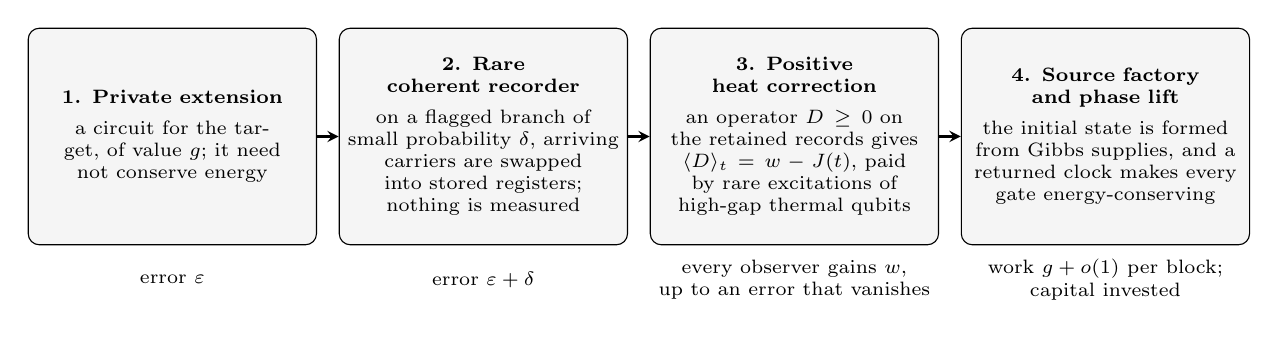
\begin{tikzpicture}[>=stealth, font=\scriptsize, stage/.style={draw, rounded corners, fill=gray!8, text width=3.45cm, align=center, minimum height=2.75cm, inner sep=3pt, anchor=north}]
  \node[stage] (s1) at (0,0) {\textbf{1. Private extension}\\[3pt] a circuit for the target, of value $g$; it need not conserve energy};
  \node[stage] (s2) at (3.95,0) {\textbf{2. Rare}\\\textbf{coherent recorder}\\[3pt] on a flagged branch of small probability $\delta$, arriving carriers are swapped into stored registers; nothing is measured};
  \node[stage] (s3) at (7.9,0) {\textbf{3. Positive heat correction}\\[3pt] an operator $D\ge0$ on the retained records gives $\langle D\rangle_t=w-J(t)$, paid by rare excitations of high-gap thermal qubits};
  \node[stage] (s4) at (11.85,0) {\textbf{4. Source factory and phase lift}\\[3pt] the initial state is formed from Gibbs supplies, and a returned clock makes every gate energy-conserving};
  \draw[->, thick] (s1) -- (s2); \draw[->, thick] (s2) -- (s3); \draw[->, thick] (s3) -- (s4);
  \node[align=center] at (0,-3.2) {error $\varepsilon$};
  \node[align=center] at (3.95,-3.2) {error $\varepsilon+\delta$};
  \node[align=center] at (7.9,-3.2) {every observer gains $w$,\\up to an error that vanishes};
  \node[align=center] at (11.85,-3.2) {work $g+o(1)$ per block;\\capital invested};
\end{tikzpicture}
\caption{The construction behind the upper bound of Theorem~\ref{to:thm:law}, read as a ledger (Appendix~\ref{to:app:schedules}). The record in stage~2 is coherent: no history is measured or postselected, and the rare branch adds only a small error. Stage~3 makes the unused part of the worst-case budget, $w-J(t)$ for the observer $t$, a positive effect on systems the device still holds, so every observer is charged the same work. Stage~4 is the finite-source and phase module of Appendix~\ref{app:module}; its capital can be enormous, but it is invested, not consumed, and comes back with the controller.}
\label{to:fig:ledger}
\end{figure}

Two remarks fix the scope for schedules that change their carriers.

\paragraph{New and retired carriers.} A schedule that delivers new output carriers, or retires inputs, needs the inventory term $(\sum_{\mathrm{new}}\ln Z_O-\sum_{\mathrm{retired}}\ln Z_I)/\beta$ in the functional; without it even the preparation of a thermal state is mispriced. The lower bound with this term holds for every schedule, since the accounting identity changes the stock's partition function by exactly this amount. In batch, for a time-covariant channel $\Phi_{A\to B}$, the corrected formula is a theorem: the capacity theorem~\cite[Thm.~7.1]{FBB21}, applied to the time-covariant channel $X_{AB}\mapsto\gamma_A\otimes\Phi(\Tr_BX_{AB})$ on the fixed composite system $AB$ with Hamiltonian $H_A+H_B$, attains it, because the capacity of that channel is $\sup_\sigma[D(\Phi(\sigma)\|\gamma_B)-D(\sigma\|\gamma_A)]$. Faist, Berta and Brand\~ao define the capacity of a channel between different systems with the unnormalized operators $e^{-\beta H}$~\cite[Eq.~(4.2)]{FBB21}, which gives this expression plus $\ln(Z_A/Z_B)$; the two differ only in how the partition functions of created and discarded systems are booked, which our contract charges through the inventory term. For general schedules with new or retired carriers, a matching construction depends on a source-formation step that we do not prove here.

\paragraph{Changing Hamiltonians.} Changes of Hamiltonian are not free relabellings: after a release, a retained switch cannot be reset between modes that assign the released system different energy gaps using only energy-conserving operations on what the device keeps, so a schedule that changes Hamiltonians must count the switch as a physical system.

% =====================================================================

\section{One functional, many schedules}\label{to:sec:table}

Most rows of Table~\ref{to:tab:corollaries} are Theorem~\ref{to:thm:law} evaluated on one schedule; the rows on exact return and on zero error lie outside its hypotheses, and the capital, bath range and lottery in the row on a clock returned approximately are not rates; these entries are listed for comparison. For a clock returned in batch, Theorem~\ref{to:thm:batchlaw} gives the same optimal rate in single-letter form, $B(\Phi)$, so the two agree. The rates in the rows on real-time channels and on a clock returned approximately are proved directly in Appendix~\ref{app:channels}, with the signed battery deviation of Table~\ref{tab:exceptions}.

\begin{table}[tbp]
\centering
\small
\begin{tabular}{>{\raggedright\arraybackslash}p{4.0cm}>{\raggedright\arraybackslash}p{3.2cm}>{\raggedright\arraybackslash}p{6.2cm}}
\toprule
Result & Schedule & Value\\
\midrule
Landauer erasure~\cite{Landauer61} & any & $\kB T\ln2$ per bit, degenerate levels\\
Batch capacity, covariant channels & hold all outputs & the capacity of~\cite{FBB21}\\
Real-time channels & release each output & $\kB T\ln2\,\Trt(\Phi)$; equal to the capacity for classical channels (Appendix~\ref{app:channels})\\
Processes with memory & interleaved & $\kB T\ln2\,K_\beta(\mathcal P)$ for every finite process (Appendix~\ref{app:module})\\
Order alone & two-step classical process & $\kB T\ln2\,[1-h_2(p)]$ per episode if released early, $0$ if held, with $p$ the bias of the process's coin (Appendix~\ref{app:module})\\
Which carriers to hold & linear task, carriers $L$ released early & $\operatorname{rank}(F_L)\,\kB T\ln2$ per use; deciding whether holding $m$ of them lowers it is NP-complete (Proposition~\ref{to:prop:rank})\\
Delayed channel & ground state first, $\Phi$ of the first input one slot later, second input discarded & $\Trt(\Phi)+\log_2\Tr e^{-\beta(H-E_0)}$ bits; the second term pays for discarding the second input (Appendix~\ref{app:module})\\
Clock returned exactly & non-covariant target & impossible at any work, with a stationary battery (Appendix~\ref{app:channels})\\
Clock returned approximately & non-covariant target & real-time rate $\Trt$; capital, bath range and lottery for gates (Appendix~\ref{app:channels} and Appendix~\ref{app:batch})\\
Batch with a returned clock & hold all, clock returned & $B(\Phi)$; the capacity when $H-\Phi^*H\in\mathrm{span}\{A_i^*A_j\}$ (Appendix~\ref{app:batch})\\
$X$-dephasing & hold all, clock returned & $E/2$, as in real time; capacity $\beta^{-1}\ln\cosh(\beta E/2)$ (Appendix~\ref{app:batch})\\
Gibbs preservation & hold all, clock returned & a positive rate per use at zero capacity (Appendix~\ref{app:batch})\\
Process vs.\ time reverse & hold all, clock returned & qutrit: $0.1547\,\kB T$ against $0$ (Appendix~\ref{app:batch})\\
Zero error, extreme channels & hold all & the full real-time rate (Appendix~\ref{app:channels})\\
\bottomrule
\end{tabular}
\caption{One functional, many schedules. Values are work per use unless marked per episode. $\Trt$, $K_\beta$ and the capacity $\mathcal T$ are in bits, to be multiplied by $\kB T\ln2$; $B(\Phi)$ and quantities written with $E$ are energies.}\label{to:tab:corollaries}
\end{table}

The real-time rate is $\Trt(\Phi)=\sup_\rho[S(\rho)-S(\Phi(\rho))+m_\rho+\beta\Tr H(\Phi(\rho)-\rho)/\ln2]$, where $m_\rho$ is the least mutual information any exact dilation must leave between the released output and what stays in the device; the thermodynamic capacity of Faist, Berta and Brand\~ao is the same expression with $m_\rho=0$~\cite{FBB19,FBB21} (Appendix~\ref{app:channels}). For processes, $K_\beta$ is an entropy change plus an energy change measured against the same adaptive observer and minimized over implementations that respect the order in which outputs are due (Appendix~\ref{app:module}). The batch quantity $B(\Phi)$ is defined in Section~\ref{to:sec:clock}.

% =====================================================================

\subsection{The channel results stated}\label{sec:channel-statements}

Four of the rows of Table~\ref{to:tab:corollaries} deserve to be stated as theorems in the main text, because they are the ones a reader is most likely to want to use. In them $\Trt$ is in bits, $B(\Phi)$ is an energy, and the capacity is written in energy units, $\kB T\ln2\,\mathcal T(\Phi)$, wherever it is compared with $B(\Phi)$. Their proofs are in Appendix~\ref{app:channels} (channels) and Appendix~\ref{app:batch} (clocks); the appendix statements carry every hypothesis.

\FloatBarrier
\begin{theorem}[Real-time work law for channels]\label{thm:main-realtime}
Let $\Phi$ be a time-covariant channel on a system with Hamiltonian $H$. In real time, the optimal work per use at vanishing error is $\kB T\ln2\,\Trt(\Phi)$, with
\[
\Trt(\Phi)=\sup_{\rho>0}\Bigl[S(\rho)-S(\Phi(\rho))+m_\rho(\Phi)+\tfrac{\beta}{\ln2}\Tr H\bigl(\Phi(\rho)-\rho\bigr)\Bigr],
\qquad
m_\rho(\Phi)=\inf_{(U,\tau)}I(O{:}E')_\rho,
\]
the infimum over finite exact dilations of the mutual information between the output and the bath output. The thermodynamic capacity is the same expression with $m_\rho=0$. Moreover, for every fixed $\delta>0$, any implementation whose controller starts thermal and that draws at most $n\kB T\ln2\,(\Trt(\Phi)-\delta)$ of deterministic work has error tending to one.
\end{theorem}

\begin{theorem}[Only quantum channels pay]\label{thm:main-dichotomy}
For repeated uses of one memoryless channel, each output released before the next input arrives, as in Theorem~\ref{thm:main-realtime}:
\begin{enumerate}[label=(\alph*),leftmargin=*]
\item If $\Phi$ is classical, meaning that it measures in an eigenbasis of $H$ and prepares states diagonal in that basis, then $\Trt(\Phi)$ equals the capacity at every temperature: waiting saves nothing.
\item For amplitude damping with probability $0<p<1$ on a qubit of gap $\Delta$, $\Trt(\Phi)=\max_{0\le y\le p}[h_2(y)-\beta\Delta y/\ln2]$ exceeds the capacity at every temperature; at $p=1$, a full reset, the two coincide.
\item For the Werner--Holevo channel $W(\rho)=(\Tr(\rho)I-\rho^T)/2$ on a qutrit with zero Hamiltonian, the real-time rate is $\log_23$ bits per use, while in batch the work is $o(n)$; at zero error a batch device too draws at least $n\log_23$ bits of free energy from its battery and controller, a bound attained with an information battery.
\end{enumerate}
\end{theorem}

\begin{theorem}[What a returned clock costs, and how large it must be]\label{thm:main-heisenberg}
Let $\Phi$ have Kraus operators $A_i$, complementary channel $\Psi$, and energy change $D=\Phi^*(H)-H$.
\begin{enumerate}[label=(\alph*),leftmargin=*]
\item \emph{Cost.} With a clock that must be returned, the batch work per use is the single-letter quantity
\[
B(\Phi)=\max_{\Psi(\rho)=\Psi(\sigma)}\Bigl\{\Tr\rho D+\kB T\ln2\bigl[S(\sigma)-S(\Phi(\sigma))\bigr]\Bigr\}\ \ge\ \text{capacity},
\]
with equality whenever $D\in\operatorname{span}\{A_i^*A_j\}$, that is, whenever some environment Hamiltonian can carry the channel's mean energy change; we call such channels balanced. The converse fails: for the Hadamard gate on a qubit of gap $E$, $D\notin\operatorname{span}\{I\}$ and yet $B(\Phi)=\text{capacity}=E/\sqrt2$, because a unitary changes no entropy and both maxima reduce to $\lambda_{\max}(D)$; for $X$-dephasing on the same qubit $B(\Phi)=E/2$ exceeds the capacity strictly.
\item \emph{Size.} When $D$ lies outside the span, the generator $i\sum_iA_i^*\dot A_i$ of the channel's time orbit $\Phi_t(\rho)=U_t\Phi(U_t^*\rho U_t)U_t^*$, $U_t=e^{-itH}$, which equals $D$, satisfies the Hamiltonian-not-in-Kraus-span condition of Zhou and Jiang~\cite{ZhouJiang21}, and the spread of the clock's capital must grow at least linearly in $n$, and at least like $n/\sqrt{\eta_n}$ when the clock is returned within $\eta_n$.
\end{enumerate}
\end{theorem}

\paragraph{Capital and implementation size.} Part~(b) of Theorem~\ref{thm:main-heisenberg} bounds the clock's capital, not the rate: the capital is invested and comes back, and part~(a) gives the work per use whatever its size. The spread is the quantity $s_n$ of Proposition~\ref{kt:prop:capital-converse}. If the controller starts in $\alpha_C=\sum_a\lambda_a|a\rangle\langle a|$ and has Gibbs state $\gamma_C=\sum_b\mu_b|b\rangle\langle b|$, it is the least mean absolute deviation of $\ln(\lambda_a/\mu_b)$ from a constant, with weights $\lambda_a|\langle a|b\rangle|^2$; for a pure controller it is $\beta$ times the mean absolute deviation of its energy from a median. The bound comes from metrology: a code built as that of Zhou and Jiang turns $n$ uses of any reliable implementation into a probe that reads the controller's clock to within $O(1/n)$ (Appendix~\ref{app:batch}). At vanishing error the clock must be broader still, with spread of order at least $n/\eta_n$ when $\varepsilon_n=O(\eta_n)$ (Proposition~\ref{kt:prop:broadclock}). When $D$ lies in the span, a clock of spread $O(\sqrt n)$ suffices for an implementation at fixed error and fixed return error (Proposition~\ref{kt:prop:clocksize}(c)), at work of order $n\log n$; whether such a clock suffices at the optimal rate is open in general (Section~\ref{sec:discussion}), and Proposition~\ref{kt:prop:reach} gives a balanced channel for which it does. For a covariant channel no clock is needed.

\begin{theorem}[Holding is decidable; releasing is not]\label{thm:main-undecidable}
In batch, a channel costs nothing with a returned clock exactly when it is Gibbs-preserving and $D\in\operatorname{span}\{A_i^*A_j\}$, a condition that linear algebra decides for channels and Hamiltonians with algebraic entries when $\beta$ is algebraic, or the Gibbs state $\gamma=e^{-\beta H}/\Tr e^{-\beta H}$ has algebraic entries (for example, every Gibbs weight $e^{-\beta E_k}$ is algebraic). In real time a channel costs nothing exactly when it is a limit of thermal operations, and there is a dimension $d_0$ such that for every $d\ge d_0$, every Hamiltonian diagonal in the dephasing basis and every temperature, no algorithm decides whether a generalized dephasing channel on $\mathbb C^d$ with cyclotomic entries is free in real time; the set of free ones is not recursively enumerable.
\end{theorem}

The batch statement needs a hypothesis on $\beta$ because Gibbs preservation involves the weights $e^{-\beta E_k}$ of the eigenvalues $E_k$ of $H$. If the Gibbs state has algebraic entries, $\Phi(\gamma)=\gamma$ is exact linear algebra over the algebraic numbers. If $\beta$ is algebraic, and nonzero as throughout, the Lindemann--Weierstrass theorem, by which $e^{\alpha_1},\dots,e^{\alpha_m}$ are linearly independent over the algebraic numbers for distinct algebraic $\alpha_k$, turns $\Phi(\gamma)=\gamma$ into the algebraic conditions $\Phi(P_k)=P_k$ for the spectral projections $P_k$ of $H$. The span condition is linear algebra over the algebraic numbers in either case.

At zero Hamiltonian and in units of purity, the rate of Theorem~\ref{thm:main-realtime}, the Werner--Holevo rate of Theorem~\ref{thm:main-dichotomy}(c) and the real-time zero set of Theorem~\ref{thm:main-undecidable} are in our earlier work~\cite{Memory,ImmediateDelivery,Douglas26closed}, and so are a strong converse at zero rate and the undecidability of that zero set when the dimension may grow~\cite{Flagship}. The batch rate of zero in Theorem~\ref{thm:main-dichotomy}(c) is the theorem of Faist, Berta and Brand\~ao, since the capacity of a unital channel at zero Hamiltonian is zero~\cite{FBB21}. Two steps are taken from our earlier preprints and not reproved here. The attainability in Theorem~\ref{thm:main-realtime}, and its formula for $m_\rho$ as an infimum over finite exact dilations, rest on the pointwise smoothing identity~\cite[Thm.~4.1, Cor.~4.3]{Douglas26closed} (Lemma~\ref{sw:lem:smoothing}). The undecidability in Theorem~\ref{thm:main-undecidable} rests on the zero-Hamiltonian closure theorem~\cite[Thm.~3.2(a)]{Memory}, which supplies the direction from zero cost to a limit of finitely factorizable channels (Step~1 of the proof of Theorem~\ref{sw:thm:undecidable}). Theorems~\ref{thm:main-realtime} and~\ref{thm:main-dichotomy} use the signed battery deviation of Table~\ref{tab:exceptions}.

The dichotomy of Theorem~\ref{thm:main-dichotomy} is the first visible consequence of the two layers of Section~\ref{sec:intro}: for a classical channel and an input diagonal in its basis, the bath can be made nearly independent of the output, by a dilation that hides the channel's randomness in a nearly flat register, so $m_\rho=0$ on such inputs. Coherent inputs can leave a positive $m_\rho$ (for complete dephasing in the computational basis at zero Hamiltonian, the input $(I+0.6X)/2$ has $m_\rho=1-h_2(0.8)\approx0.28$ bits), but they cannot raise the optimized real-time cost, so the real-time rate is the capacity (Appendix~\ref{app:channels}). For a quantum channel such as partial reset the output is necessarily correlated with what is left behind. The dichotomy concerns memoryless channels: a classical process with memory can pay for release, as the task of Figure~\ref{fig:three} does (Section~\ref{sec:classes}). Theorem~\ref{thm:main-heisenberg} says that the clock-size question and the metrology question have the same answer for the same reason: inputs that the environment cannot tell apart but that differ in energy are exactly the inputs that make a code sensitive to the channel's phase, as in the code of Zhou and Jiang~\cite[Sec.~V]{ZhouJiang21}. Whether the clock also costs work above the capacity is a separate question, decided by $B(\Phi)$ and not by the span alone.

\section{What waiting buys}\label{to:sec:waiting}

\paragraph{Side information.} Take a memory $M$ whose states all have the same energy, as in an information register, and many copies of a fixed state of $M$ and its quantum side information $O$. Erasing $M$, while leaving $O$ and its correlations with everything else intact, costs $\kB T\ln2\,S(M|O)$ per copy; del Rio et al.\ showed that this much work suffices, even when it is negative~\cite{delRio11}. Without the side information it costs $\kB T\ln2\,S(M)$, more by the mutual information $I(M{:}O)$. When the states of $M$ differ in energy, the reset changes that energy too, and the cost changes with it. A qubit of gap $E$ at $\beta E=\ln2$, in its Gibbs state, is excited with probability $1/3$; resetting it to its ground state costs $\kB T\ln2\,[h_2(1/3)-1/3]=\kB T\ln(3/2)$, that is $0.585$ bits per copy, not the $h_2(1/3)=0.918$ bits of its entropy. This is the rate of a full reset, Theorem~\ref{thm:main-dichotomy}(b) at $p=1$, whose hardest input is this Gibbs state. The law of Section~\ref{to:sec:law} and the integrands below include this energy term. A batch device keeps its outputs as side information until it has cleaned up~\cite[Sec.~7]{FBB21}; a real-time device has already released them. At a fixed input $\rho$, the real-time integrand exceeds the batch one by $m_\rho$, the least such mutual information an implementation must leave, which can be smaller than any particular dilation suggests. For time-covariant channels the optimal batch rate in this thermal-operation model is the thermodynamic capacity $\mathcal T(\Phi)=\max_\rho c_\rho$, where $c_\rho=S(\rho)-S(\Phi(\rho))+\beta\Tr H(\Phi(\rho)-\rho)/\ln2$, so the surcharge between the optimal rates is $\Trt(\Phi)-\mathcal T(\Phi)=\max_\rho(c_\rho+m_\rho)-\max_\rho c_\rho$. It is not an optimum of $m_\rho$ alone, because the two maxima can sit at different inputs. The extra term $m_\rho$ is a correlation cost, input by input; the surcharge compares two optimized totals. For amplitude damping at $p=1/2$ and $\beta E=\ln2$ (Figure~\ref{to:fig:surcharge}), $m_\rho=0.918$ bits at the real-time optimum, while the surcharge is $0.585E-0.154E=0.431E$ per use, that is $0.431$ bits. For a general channel with a returned clock the batch endpoint is instead $B(\Phi)$ of Section~\ref{to:sec:clock}, and the saving from waiting is $\kB T\ln2\,\Trt(\Phi)-B(\Phi)$. The capacity gap remains a benchmark, but it need not be a saving available under that return contract: $X$-dephasing costs $E/2$ per use in both schedules, above its capacity. On inputs diagonal in its basis, a classical channel can leave behind nothing correlated with the outputs it releases, by hiding its randomness in a nearly flat register; coherent inputs can leave a correlation, but they cannot raise the optimized cost (Appendix~\ref{app:channels}). So a classical channel pays nothing extra, much as an information ratchet avoids modularity dissipation by designing internal states that capture the global correlations~\cite{BMC18}; a quantum channel such as partial reset of a qubit must leave its output correlated with what remains, and pays a surcharge at every temperature (Appendix~\ref{app:channels}). Only quantum channels save work by waiting. Here a channel means repeated uses of one memoryless map: classical tasks with several steps can also save work by waiting, as Proposition~\ref{to:prop:rank} shows exactly. This concerns the channel, not the memory: for classical strategies with stochastic outputs, a quantum memory can lower the online cost below that of every classical agent whose memory is a function of the past~\cite{Thompson25}, and only when two causal states form a causally wasteful pair~\cite[Result~2]{Thompson25}.

\begin{figure}[t]
\centering
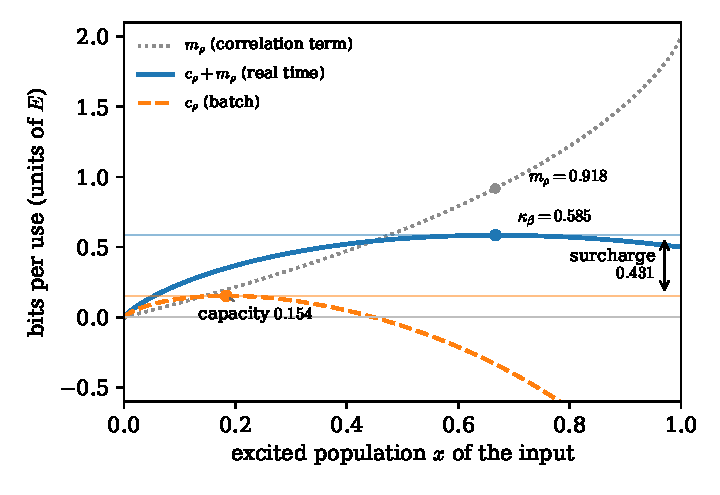
\includegraphics[width=0.62\linewidth]{fig-surcharge.pdf}
\caption{The surcharge is a difference of two maxima. Amplitude damping with $p=1/2$ at $\beta E=\ln2$, so that one bit costs $E$; inputs diagonal in the energy basis, with excited population $x$, attain both maxima. Dashed: the batch integrand $c_\rho=h(x)-h(x/2)-x/2$, whose maximum is the capacity, $0.154$, at $x\approx0.18$. Solid: the real-time integrand $c_\rho+m_\rho=h(x/2)-x/2$, whose maximum is $\Trt=0.585$, at $x=2/3$. Dotted: the correlation term $m_\rho=2h(x/2)-h(x)$. The surcharge, $0.431$, is neither $m_\rho$ at the real-time optimum, $0.918$, nor $m_\rho$ at the batch optimum, $0.197$.}
\label{to:fig:surcharge}
\end{figure}

\paragraph{Error.} For extreme channels, the batch saving requires nonzero error, even when that error vanishes with the block size.

\begin{proposition}[Zero error removes the saving for extreme channels (Appendix~\ref{app:channels})]\label{to:prop:extreme}
If a channel is extreme in the convex set of channels, every implementation with zero error, in batch or in real time, draws free energy from its battery and controller at no less than the real-time rate.
\end{proposition}

Extremality makes the branches of any exact implementation orthogonal~\cite{Choi75}, so the device's entropy rises by exactly the entropy of the complementary output on every input. For amplitude damping at $p=1/2$ and $\beta E=\ln2$, the real-time rate is $0.585\,E$ per use and the batch capacity $0.154\,E$ (Appendix~\ref{app:channels}); the difference is available only to a device that tolerates some error.

\paragraph{Delay.} Let each output be released $b$ steps later than in real time. For independent delayed-choice episodes, in which a qubit is released and the question it must answer arrives $\ell_i$ steps later, the number of episodes that still require an early commitment is $\#\{i:\ell_i>b\}$, and under one-way communication from the party that answers, the entanglement cost is exactly this number (a question that arrives in the same step as the delayed release is taken to arrive first): each such episode is charged one ebit by the monogamy argument of Section~\ref{to:sec:beyond}, and every other episode is answered before its release at no cost. One more step of delay saves $\#\{i:\ell_i=b+1\}$: a step of delay is worth exactly the questions it moves to the accessible side of a release, and has no fixed exchange value. Under the strict real-time rule, where the next input arrives only after the last output has left, waiting longer does not move any question and buys nothing. For repeated uses of one channel, running blocks in batch, with the exponentially small block error that the construction of Faist, Berta and Brand\~ao has at a fixed typicality tolerance (proof of Theorem~\ref{sw:thm:werner}), and taking a union bound over blocks comes within any fixed $\delta>0$ of the batch rate once the delay exceeds $C_\delta\log(n/\varepsilon)$; this construction reaches the batch rate itself only with a delay that grows faster than $\log(n/\varepsilon)$, and the exact work--latency profile is open.

\paragraph{Which carriers to hold.} With several carriers in flight, a schedule can let some of them wait for a later input while others leave. For linear tasks the price of such a schedule is a rank, and the best choice of what to hold is a question about codes. For example, let the late output need the two parities $a_1\oplus a_2$ and $a_2\oplus a_3$, so that $F$ has rows $(1,1,0)$ and $(0,1,1)$. Releasing all three bits costs two bits. Holding any one of them still leaves released columns of rank two, so it saves nothing; holding any two leaves a single nonzero column and lowers the cost to one bit; holding all three makes it zero. A held bit helps only when it completes a late parity, not merely because it is one more bit of storage.

\begin{proposition}[Release rank]\label{to:prop:rank}
Let $F$ be an $\ell\times k$ binary matrix. A device receives $a\in\mathbb F_2^k$ on $k$ bit carriers with zero Hamiltonian. The carriers in a set $L$ must leave, unchanged, before a fresh $b\in\mathbb F_2^\ell$ arrives on $\ell$ further carriers; those in $R=\{1,\dots,k\}\setminus L$ may be held until then. In the end the device returns every first carrier unchanged and dephased, and the second carriers holding $b\oplus Fa$. Let $D$ be everything the device keeps, initially independent of the inputs, and let $F_L$ be the columns of $F$ in $L$.
\begin{enumerate}[label=(\alph*)]
\item For independent uniform $a$ and $b$, every exact implementation raises the entropy of $D$ by at least $\operatorname{rank}F_L$ bits, so, when its controller, battery and Gibbs reservoirs start independent, it dumps heat at least $[\operatorname{rank}F_L-\Delta S_C-\Delta S_W]\,\kB T\ln2$, with $\Delta S_C$ and $\Delta S_W$ the entropy changes of its controller and battery in bits. An energy-conserving implementation raises the entropy by exactly $\operatorname{rank}F_L$ and dumps heat $(1-q)\operatorname{rank}(F_L)\,\kB T\ln2$, where $q$, the probability that its battery misses its final level, can be made as small as desired.
\item If any $m$ carriers may be held, the least cost is $\operatorname{rank}F-\max\{r:d_r(\mathcal C)\le m\}$ bits, where $\mathcal C$ is the row space of $F$ and $d_r(\mathcal C)$, its $r$-th generalized Hamming weight, is the smallest support of an $r$-dimensional subcode~\cite{Wei91}. Holding $m$ carriers lowers the cost at all exactly when $\mathcal C$ has a nonzero word of weight at most $m$, which is NP-complete to decide~\cite{Vardy97}.
\end{enumerate}
\end{proposition}

Holding every carrier costs nothing, and holding one more carrier helps only when it completes a late parity, one that then depends on held carriers alone: the price $\operatorname{rank}F_L=\operatorname{rank}F-\dim\mathcal C(R)$ counts the independent parities of the released bits that the late output still needs, where $\mathcal C(R)$ is the set of late parities supported on held carriers. By part (b), the price of a schedule is a coding invariant of the task: its generalized Hamming weights, which Wei introduced for the wire-tap channel of type II~\cite{Wei91}. The proof is in Appendix~\ref{to:app:rank}.

% =====================================================================
\section{Returning a clock}\label{to:sec:clock}

A channel that is not time-covariant needs a phase reference. If the reference is finite-dimensional and must come back exactly, and the battery is stationary, no such channel can be run at any work cost: by the no-broadcasting theorem for asymmetry, a bounded reference used to implement an operation that is not covariant is necessarily degraded~\cite{MarvianSpekkens19,LostaglioMuller19}; if it need only come back approximately, every channel runs in real time at the rate $\Trt$ (Appendix~\ref{app:channels}, with the signed battery deviation of Table~\ref{tab:exceptions}). For a gate the reference then pays in other currencies: capital at least of order $n/(\varepsilon+\eta)$, baths whose energy range grows at least like $n/\sqrt\varepsilon$, and an energy that returns only as a lottery (Appendix~\ref{app:batch}). The capital has the scaling of the reference-size laws of Chiribella, Yang and Renner and of Tajima, Shiraishi and Saito~\cite{ChiribellaYangRenner21,TSS20}. Channels that are not gates can need far less: a Gibbs-preserving qubit channel that is not time-covariant runs in batch at zero work with a clock whose spread grows like $\sqrt n$ (Appendix~\ref{app:batch}).

In batch the returned clock has an exact price. Let $\Psi$ be a complementary channel, $D=\Phi^*(H)-H$ and
\[
B(\Phi)=\max\bigl\{\Tr\rho D+\kB T\ln2\,[S(\sigma)-S(\Phi(\sigma))]\;:\;\Psi(\rho)=\Psi(\sigma)\bigr\}.
\]

\begin{theorem}[The batch law with a returned clock (Appendix~\ref{app:batch})]\label{to:thm:batchlaw}
With a battery that starts in an energy eigenstate and a controller that returns approximately, all of it and not only the clock, the optimal batch work per use of every finite channel is $B(\Phi)$, attained with deterministic work. It equals $\kB T\ln2\,\mathcal T(\Phi)$, the thermodynamic capacity in energy units, whenever $D$ lies in the span of the products $A_i^*A_j$ of Kraus operators, and a Gibbs-preserving channel is free exactly when it does.
\end{theorem}

Two inputs can be charged separately, one for energy and one for entropy, exactly when the environment cannot tell them apart. When the environment can carry the energy change, input by input on average, the clock never has to absorb an energy that depends on the input, and the capacity is reached. This makes precise the obstruction that Faist, Berta and Brand\~ao anticipated: for superposed inputs of different energy, the environment must compensate the energy difference without disturbing the process~\cite{FBB19}. A returned clock can supply phase, but it cannot provide net extensive energy: for every observer its actual mean energy change must be sublinear. It can still make large loans that depend on the branch, as long as their mean is refunded. When the environment cannot carry the energy change, the remainder may have to be paid, but it need not be: a unitary gate changes no entropy, so for the Hadamard gate $B(\Phi)$ equals the capacity although $D$ lies outside the span (Section~\ref{sec:channel-statements}). Qubit dephasing in the $X$ basis costs $E/2$ per use in batch, exactly its real-time cost and above its capacity; some Gibbs-preserving channels, of capacity zero, cost work of order $n$; and every Gibbs-preserving qubit channel is free in batch with a returned clock (Appendix~\ref{app:batch}). The span of the products $A_i^*A_j$ is the non-commutative confusability graph of Duan, Severini and Winter~\cite{DSW13}. The same condition separates small clocks from large ones. When $D$ lies outside the span, the channel's orbit under time translation, whose generator is exactly $D$, can be estimated at the Heisenberg limit~\cite{ZhouJiang21}. A code built as in~\cite[Sec.~V]{ZhouJiang21} turns $n$ uses of any reliable implementation into a probe that reads the controller's clock to within $O(1/n)$, so no clock whose spread grows more slowly than $n$ can run it reliably, at any work (Appendix~\ref{app:batch}).

\begin{table}[tbp]
\centering
\small
\begin{tabular}{>{\raggedright\arraybackslash}p{4.6cm}>{\raggedright\arraybackslash}p{6.6cm}l}
\toprule
Schedule and clock & Processes that cost nothing & Decidable\\
\midrule
Batch, Gibbs-preserving maps free~\cite{FBB21} & Gibbs-preserving channels & yes\\
Batch, clock returned & Gibbs-preserving, with $H-\Phi^*H\in\mathrm{span}\{A_i^*A_j\}$ & yes\\
Real time & limits of thermal operations (Appendix~\ref{app:channels}) & no\\
\bottomrule
\end{tabular}
\caption{The free channels shrink as the operational model tightens: Gibbs-preserving maps taken as free operations, thermal operations with a returned clock in batch, and thermal operations in real time. Each inclusion is strict: a Gibbs-preserving qutrit separates the first two rows (Appendix~\ref{app:batch}), the Werner--Holevo channel, which is not factorizable~\cite{HaagerupMusat11}, the last two. Decidability is for exact algebraic data, under the hypothesis of Theorem~\ref{thm:main-undecidable}.}\label{to:tab:ladder}
\end{table}

\paragraph{A process and its time reverse.} For a Gibbs-preserving channel, the reverse process of quantum fluctuation theorems~\cite{Crooks08,KwonKim19} is its Petz map $\Phi^\sharp(\sigma)=\gamma^{1/2}\Phi^*(\gamma^{-1/2}\sigma\gamma^{-1/2})\gamma^{1/2}$. Thermal operations are closed under this reversal. With a returned clock, the criterion of Theorem~\ref{to:thm:batchlaw} is not: on a qutrit there is a Gibbs-preserving channel that costs $0.1547\,\kB T$ per use while its reverse costs nothing (Appendix~\ref{app:batch}). Which direction is free is decided by two linear tests on the Kraus operators. The asymmetry is not generic: channels of full Kraus rank pass both tests, so any fixed amount of full-rank thermal noise removes it, and separated pairs lie on the boundary of the set of Gibbs-preserving channels, as Tajima and Takagi found for Gibbs-preserving maps whose coherence cost diverges~\cite[Suppl.\ Prop.~S.11]{TajimaTakagi25}. For a finite device the threshold is set by the horizon: noise removes the asymmetry only when the expected number of noisy uses grows without bound, so noise per use small compared with the inverse of the number of uses leaves the full cost in place (Appendix~\ref{app:batch}). In coherence the same pair is already asymmetric, as Tajima and Takagi found for detecting versus creating coherence~\cite{TajimaTakagi25}: by their theorem the forward channel, which keeps a pair of orthogonal coherent inputs perfectly distinguishable, needs coherence that diverges as the error vanishes, while its reverse, which reads energy populations and prepares coherent states, can be implemented with finite coherence by the construction they give for maps of that kind~\cite[Suppl.\ Sec.~IV]{TajimaTakagi25}. With a returned clock the asymmetry appears in work. It is an implementation asymmetry created by the obligation to return the clock. It does not violate any fluctuation theorem, and it is not carried by the clock, whose entropy changes by $o(n)$.

% =====================================================================

\section{What a released past must keep}\label{sec:classes}

The two-bit example of Figure~\ref{fig:three} has a general form, and it is the cleanest place to see the mechanism of the law without any quantum ingredient. A past $x$ arrives and must be released. Later a question $y$ arrives, and the device must answer it with $g(x,y)$. Two things can cost work here, and it pays to keep them apart. One is ordinary erasure: if the answer discards part of $y$, the device must absorb what it discards, whatever the schedule. The other is order: while $x$ is gone, the device must still be able to answer every $y$, so it must keep a record of what $x$ can still tell apart. The theorem below prices both and separates them.

\paragraph{Classes and fibers.} Fix nonempty finite alphabets $X,Y,Z$ and $g:X\times Y\to Z$. Two pasts are \emph{equivalent}, $x\sim x'$, if $g(x,\cdot)=g(x',\cdot)$: no later question distinguishes them. Let $K(g)$ be the number of classes, $c(x)$ the class of $x$, and write $g(c,y)$ for the common value on a class. Two counts measure what an answer discards:
\[
F(g)=\max_{x\in X,\ z\in Z}\bigl|\{y:g(x,y)=z\}\bigr|,
\qquad
F'(g)=\max_{z\in Z}\bigl|\{(c,y):g(c,y)=z\}\bigr| .
\]
$F$ is the most questions a single past leaves indistinguishable after answering; $F'$ counts pairs of a class and a question that lead to the same answer. Always $F\le F'\le K\,F$. A task has \emph{reversible questions} if $y\mapsto g(x,y)$ is a bijection of $Y$ onto $Z$ for every $x$; then $F=1$ and $F'=K$. The classes are the distinct rows of the table of $g$, so $\lceil\log_2K(g)\rceil$ is the deterministic one-way communication complexity of $g$ from the party that holds the past~\cite{KushilevitzNisan96}; read as a strategy, they are its causal states, the memory states of an optimal causal agent in computational mechanics~\cite{BarnettCrutchfield15,Thompson25}. Thompson et al.\ price such agents for a given input process, with each question kept on the tape and each answer written to a fresh cell~\cite{Thompson25}. There the record can be uncomputed against the question and the answer, and the cost they find is the information the memory stores about the last input and output minus what it holds about the next ones~\cite[Eq.~(3)]{Thompson25}, nonpredictive information of the kind that Still, Sivak, Bell and Crooks identified with the average dissipation of a system driven by a stochastic signal~\cite{Still12}; for the task of Figure~\ref{fig:three} that cost is zero. Here the answer overwrites the question, as in the information ratchets of~\cite{BMC18}, and the price is a worst case over observers; Appendix~\ref{app:module} compares the two interfaces.

\begin{theorem}[Fiber law for a released past]\label{thm:classes}
Let the task $T_g$ be: a carrier arrives holding $x$ in the computational basis, is dephased and released; a second carrier, of dimension $\max\{|Y|,|Z|\}$, then arrives holding $y$ and must be released holding $g(x,y)$; its admissible inputs, together with the observer's references, are supported on $\operatorname{span}\{|y\rangle:y\in Y\}$ tensored with the references, a promise that is part of the task. All carriers have zero Hamiltonian. Against quantum devices and observers with references,
\begin{align*}
K_\beta^{S}(T_g)&=\log_2F'(g)\quad\text{bits per episode in real time},\\
K_\beta^{S}(T_g)&=\log_2F(g)\quad\ \text{bits per episode when $x$ may be held until $y$ arrives.}
\end{align*}
The order price, the difference, lies between $0$ and $\log_2K(g)$. For reversible questions it is $\log_2K(g)$ and the held price is zero. For a constant answer $g\equiv z_0$ it is zero, and both schedules pay $\log_2|Y|$: the Landauer cost of erasing $y$.
\end{theorem}

The proof is in Appendix~\ref{app:classes}; its two halves are the two halves of Theorem~\ref{to:thm:law}. The upper bound is a device that dephases each carrier with a coin drawn from the reservoir, writes the class $c(x)$ into a register before $x$ leaves, and when $y$ arrives rewrites $(c,y)$ reversibly as the answer $g(c,y)$ on the carrier and an index of the pair within the fiber of that answer in the register; the index has at most $F'$ values. The lower bound needs two kinds of observer. Observers who might ask a distinguishing question force the device to know the class of $x$ at the moment $x$ leaves, since one fixed later operation must tell the classes apart. The \emph{steering} observer (it steers the answer; the word has nothing to do with quantum steering), who chooses the answer $z_0$ with the largest fiber and sends pasts and questions uniformly over that fiber, then leaves the device no way to pass that knowledge on, because every answer it returns is $z_0$. An identity for the information the device holds about the observer's choices, visit by visit, turns these two facts into an entropy increase of $\log_2F'$ per episode, up to the explicit loss $\delta_g(\varepsilon)$ for sufficiently small $\varepsilon$, uniform in the number of episodes and in the dimension of the private device. The held bound is the thermodynamic capacity of the classical channel $(x,y)\mapsto(x,g(x,y))$, which is $\log_2F$. Both prices are worst-case Landauer costs of one logical operation applied in the same way to every input, $(x,y)\mapsto(x,g(x,y))$ when the past is held and $(c,y)\mapsto g(c,y)$ in real time, the setting of the general forms of Landauer's principle for deterministic and indeterministic operations~\cite{Turgut09,Maroney09}. Merging of this kind has also been priced for finite automata that read their input once, in real time: K{\i}yak and Say charge such an automaton $\log_2P$ bits whenever it reaches a configuration with $P$ possible predecessors, and compare deterministic automata with quantum automata at zero and at bounded error~\cite{KiyakSay24}. Their automaton has a fixed finite memory and is charged step by step for recognizing a language; here the device may have any size, the price is a rate against the worst observer, and the real-time bound holds against every quantum device at small error. What the real-time bound adds is the continuation constraint of a released past, which forces the record of the class, and the pairing of observers that prices that record robustly.

\paragraph{Release rank is the linear case.} When $X=\mathbb F_2^k$, $Y=Z=\mathbb F_2^m$ and $g(x,y)=y+Fx$, the questions are reversible, the classes are the cosets of $\ker F$, and the order price is $\operatorname{rank}(F)$ bits. With several input carriers in flight, some of which may be held, Proposition~\ref{to:prop:rank} gives the price as the rank of the released part $F_L$ and shows that deciding whether holding $m$ carriers lowers it at all is NP-complete.

\paragraph{A record is not yet a price.} The record of $c(x)$ must exist at the moment $y$ arrives, whatever $y$ turns out to be: for pasts in different classes the device's states at that moment are told apart by one fixed later operation, so they are orthogonal, and nearly so at small error (Lemma~\ref{lem:classes-orth}). It is tempting to conclude that the device pays $\log_2K$ against every observer, including one who never asks a distinguishing question. That conclusion is false, and the reason is instructive. For the XOR task the reversible two-gate circuit
\[
(M,Y)=(a,y)\ \longmapsto\ (y,\ a\oplus y)
\]
answers every question correctly and leaves the register holding $y$ rather than $a$: the record of the past has been passed into the answer, as in a reversible computation that uncomputes its history~\cite{Bennett73}. Against an observer who always sends $y=0$ this device ends each episode with an empty register and pays nothing. What the law charges is the entropy the device cannot pass on, and the lower bound pairs the observers who might ask a distinguishing question, which force the record to exist, with the observer who closes the only exit by choosing questions that make the answer constant. Neither suffices alone: for $g(x,y)=x\wedge y$ a device that serves only the steering observer pays $h_2(1/3)\approx0.918$ bits per episode instead of $\log_23$. The price is a property of the worst observer the device must serve, not of the record it must hold.

\paragraph{Order prices are not additive.} One might hope to price a schedule by a sum of terms, one per release decision. For linear tasks the price is a rank function and is submodular in the released set. For reversible tasks in general it is not: in Appendix~\ref{app:classes}, Proposition~\ref{prop:nonsubmodular} gives a task on three bits with a three-valued answer whose order price violates submodularity by $\log_2(3/2)$ bits per episode, the largest for any task of the form $g(x,y)=y+f(x)\bmod3$ on three bits. What is additive is the law itself, across independent episodes, which is why rates are the right object.

\section{Holding is decidable, releasing is not}\label{to:sec:computability}

In batch, whether a channel costs nothing is decided by linear algebra for exact algebraic data under the hypothesis of Theorem~\ref{thm:main-undecidable}: Gibbs preservation, and with a returned clock the span condition of Theorem~\ref{to:thm:batchlaw}. For a channel, Hamiltonian and temperature given exactly, for example with algebraic entries, the batch cost with a returned clock, $B(\Phi)$, is a finite-dimensional optimization that can be computed to any precision; unlike the capacity, it is not continuous in the channel, so it cannot be estimated uniformly from approximate data. In real time, a channel costs nothing exactly when it is a limit of thermal operations, and no algorithm decides membership, even in a fixed dimension (Appendix~\ref{app:channels}), extending the zero-Hamiltonian result of~\cite{Flagship}. Choosing what to hold is hard in a different way: for the linear tasks of Proposition~\ref{to:prop:rank} the cost of each choice is a rank, computable in polynomial time, but deciding whether holding $m$ carriers lowers it at all is NP-complete.

The source of the undecidability is the absence of a computable bound on the size of the noncommutative dilations that witness membership. It is present already at zero Hamiltonian, where the question becomes whether a channel is a limit of finitely factorizable ones~\cite{Memory}, so Gibbs weights are not essential. It is also not a consequence of time order alone. Under local operations and classical communication, a channel is free in batch exactly when it is entanglement-breaking~\cite{HSR03},~\cite[Cor.~18]{BBCW13}, and so also in real time; this is a semialgebraic condition, decidable by quantifier elimination. Under one-way communication from the party that answers, a delayed-choice task is free in real time exactly when its assemblage has a local-hidden-state model, the free assemblages of the resource theory of steering~\cite{GallegoAolita15}; this is a semidefinite condition~\cite{CavalcantiSkrzypczyk17}. Outside that set, squashed entanglement is bounded below by a constant times the squared distance to the separable states in a one-way LOCC norm, with no dependence on dimension~\cite{BCY11}, so the rate is positive. Under incoherent operations a delayed-choice task is free exactly when its conditional states are diagonal. Unbounded free ancillas are not enough to make freeness undecidable. Among the theories treated here, thermodynamics is the one in which releasing in time makes the zero set uncomputable.

What the results show is operational. Being able to describe every event at once does not mean being able to act on every event at once. The difference has a price, and in thermodynamics whether that price is zero cannot be computed.

% =====================================================================

\section{Speed, order and a measurement}\label{to:sec:measure}

\paragraph{Speed and order together.} Output deadlines alone impose no deadline on preparation or cleanup: a device can prepare its resources in advance, release its outputs on time and restore itself slowly afterwards. In our model the order cost is therefore pure order. A speed price appears only when the thermal interface is budgeted. Consider a collision model in which each thermal contact fully swaps one cell with a fresh Gibbs qubit. Let a device implement the target at error $\varepsilon$, and let it reset its cells along strokes of thermodynamic length $\ell_j$, each a cooling stroke that starts at excited population at most $1/2$, using $K_j$ contacts per stroke and no other operation on the cell during a stroke. Each contact is a step equilibration, and for a process carried out in $K$ such steps the dissipation is at least $\kB T\ell^2/(2K)$ to leading order in $1/K$, for thermodynamic length $\ell$~\cite{SalamonBerry83,Nulton85,Crooks07,ScandiPerarnauLlobet19,Abiuso20}. For these strokes the bound holds exactly at every $K_j$, as shown below, and summing over strokes gives
\[
W\ \ge\ W^{\mathrm{qs}}(\varepsilon)+\frac{\kB T}{2}\sum_j\frac{\ell_j^2}{K_j}\ \ge\ W^{\mathrm{qs}}(\varepsilon)+\kB T\,\frac{(\sum_j\ell_j)^2}{2K_{\mathrm{tot}}},
\]
where $W^{\mathrm{qs}}(\varepsilon)$ is the slow limit of the same device. For a device that attains its schedule's optimum it tends to $W^{\mathrm{qs}}_{\mathrm{batch}}+W_{\mathrm{order}}$ as $\varepsilon\to0$; any other device adds its own implementation overhead. For other strokes, including recoveries that extract work, the factor $1/2$ holds only to leading order in $1/K_j$; the factor $1/4$ holds exactly. Both exact statements have short proofs. A stroke whose contacts take the cell through the excited populations $a=q_0,q_1,\dots,q_K=b$ dissipates $\kB T\sum_jd(q_{j-1}\|q_j)$, with $d$ the binary relative entropy in nats, and $\ell=2|\theta(a)-\theta(b)|$ with $\theta(q)=\arcsin\sqrt q$. Jensen's inequality gives $d(p\|q)\ge-2\ln\cos(\theta(p)-\theta(q))\ge(\theta(p)-\theta(q))^2$ for every step, and Cauchy--Schwarz over the $K$ steps gives the factor $1/4$. For $q<p\le1/2$ the difference $d(p\|q)-2(\theta(p)-\theta(q))^2$ vanishes at $q=p$ and has derivative $[2(\theta(p)-\theta(q))-(p-q)/\sqrt{q(1-q)}]/\sqrt{q(1-q)}\le0$ in $q$, since $2(\theta(p)-\theta(q))=\int_q^p dx/\sqrt{x(1-x)}$ and $x(1-x)$ increases on $[0,1/2]$; so a downward step within $[0,1/2]$ costs at least $2(\theta(p)-\theta(q))^2$. In a cooling stroke from $a\le1/2$ to $b$, raising every population to at least $b$ and then replacing the path by its running minimum raises no step's cost and leaves only downward steps within $[b,a]$, and Cauchy--Schwarz gives the factor $1/2$. When ordinary and order-forced resets, of total lengths $L_B$ and $L_O$, share one budget of $M$ contacts, the least dissipation is $\kB T(L_B+L_O)^2/(2M)$ to leading order in $1/M$, with the contacts split in the ratio $L_B:L_O$. Two separate interfaces with the same total of $M$ contacts reach the same value when they split them in that ratio, so sharing an interface adds no cross term of its own; the difference $\kB T\,L_BL_O/M$ from $\kB T(L_B^2+L_O^2)/(2M)$ arises only against separate interfaces granted $M$ contacts each, $2M$ in all. The order-forced resets lengthen the path the contact budget must cover. Order decides which resets must happen; speed charges for completing them in time. At a fixed number of contacts, driving the error to zero makes the work diverge, as finite resources forbid a perfect reset~\cite{ReebWolf14,Taranto23}, although only logarithmically for a single contact and far more slowly for several. Any finite law must therefore state its error.

\paragraph{A measurement.} Measure the work as a function of the thermal-contact budget $K$ for both schedules at the same certified error. Fit each curve by an intercept plus terms in $1/K$ and $1/K^2$, or by the exact finite-$K$ curve of the collision model, as tests of Landauer's principle extrapolate the work to slow operation~\cite{Berut12,Jun14}. The difference between the two slow-limit intercepts is the excess quasistatic work of the two implementations at the certified error. It equals the order surcharge only when both implementations attain their schedule optima; otherwise it also contains implementation overhead, and the finite certificates below give an unavoidable lower bound without any such optimality claim. The slopes carry speed. Near a pure target the work approaches its $1/K$ law slowly: in the collision model above, for the amplitude-damping example below with a cell reset from its Gibbs state to excited population $10^{-6}$, a fit with $1/K$ alone over budgets of four to twelve contacts biases the intercept by about a tenth of the order cost, and adding the $1/K^2$ term, or fitting over ten to fifty contacts, brings the bias to about one percent. For amplitude damping at $p=1/2$ and $\beta E=\ln2$, the difference for many uses at vanishing error is $0.4313\,E$ per use, about $1.4\times10^{-24}$\,J at $5$\,GHz with a local reservoir at $346$\,mK. Over a finite number of uses it is smaller, and for a single use it vanishes.

\paragraph{Cautions.} Three cautions apply. First, at that temperature a $5$\,GHz bath implements generalized amplitude damping, so the target channel needs an engineered reservoir whose cost is counted. At impurity $10^{-6}$ the last thermal carrier needs a gap near $100$\,GHz, unless an encoded carrier or a costed colder reservoir is used. Second, amplitude damping is extreme, so its batch saving exists only at nonzero error, and both intercepts depend on that error. Third, the decisive comparison needs finite certificates for the implemented devices, not asymptotic rates.

\paragraph{Finite certificates.} Two finite certificates exist. One is a saving at $256$ uses and error $10^{-8}$ (Appendix~\ref{app:channels}); it needs reservoirs far too large to build. The other is the two-qubit process of the introduction, and it does not.

\begin{proposition}[A two-qubit certificate]\label{to:prop:certificate}
Two qubit carriers $A$ and $B$ with zero Hamiltonian, which are also the output carriers, arrive in turn, and the target $\mathcal P$ removes the coherences of the inputs and sends $|ab\rangle$ to $(I\otimes X^b)(|00\rangle+(-1)^a|11\rangle)/\sqrt2$. Energies are in units of $\kB T\ln2$ and entropies are in bits.
\begin{enumerate}[label=(\alph*), leftmargin=*]
\item \emph{Held.} If $A$ may be held until $B$ arrives, $\mathcal P$ is implemented exactly with no work and no heat: two controlled-$Z$ gates driven by maximally mixed coins, a Hadamard and a CNOT.
\item \emph{What is measured.} Feed $A=|0\rangle$ and, after $A$ has left, $B$ as half of a maximally entangled pair whose other half $Q$ the observer keeps. The leakage $e$ out of the two-dimensional code of ideal outputs on this probe is fixed by three local Pauli settings, and two bound it: $e\le\Pr[X_AX_B=-1]+\Pr[Z_QZ_AZ_B=-1]$. At strategy error $\varepsilon$, $e\le\varepsilon$.
\item \emph{Work.} Let an early-release implementation have a controller, Gibbs reservoirs at temperature $T$ and a sharp battery that start independent, and on this probe let the changes of the controller's energy and entropy, the battery's entropy, and the battery's mean deviation from its nominal debit total at most $P$. Then its nominal work per episode is at least $1-h_2(e)-e\log_23-P$.
\item \emph{Heat.} No entangled probe is required. For independent probe states, let the device's parts and a monitored bath at temperature $T$ start independent, the bath in its Gibbs state. The net heat into that bath per episode is at least $S(\rho_A)+S(\rho_B)-H_4(p)-\Delta S_C-\Delta S_W-\Delta S_{\rm other}$, where $p$ is the distribution of the two stabilizers above, $H_4(p)\le h_2(e)+e\log_23$, and $\Delta S_C$, $\Delta S_W$ and $\Delta S_{\rm other}$ are the entropy changes of the controller, the battery and every other sink. This form needs no refund of the controller's energy and no sharp battery.
\end{enumerate}
\end{proposition}

The proof is in Appendix~\ref{to:app:certificate}. With $P=0.025$, the work bound of (c) is more than $0.87$ at $\varepsilon=10^{-2}$ and more than $0.05$ up to $\varepsilon\approx0.169$, against $0$ for the held process, and it is tight as $\varepsilon$ and $P$ vanish. For the heat form, let the probe of $B$ be a uniformly random classical bit that the observer records, drawn fresh in every episode, independently of the device's state. A device with memory that knew the setting could tailor its output to it, so the observer chooses the setting of each episode at random, independently of the device's history, and keeps it hidden until both outputs of the episode have been released; every setting then samples the same average conditional emitted state. Take $150{,}000$ episodes, fixed in advance, about $50{,}000$ per setting. With $5\%$ observed leakage, the Hoeffding--Azuma inequality~\cite{Hoeffding63,Azuma67}, which holds when the device carries memory across episodes, keeps the run's average leakage below $7\%$ except with probability below $3\times10^{-4}$. At an average leakage of $7\%$, with a readout calibrated for every input state, a preparation entropy of $0.99$ bits and $0.08$ bits of entropy allowed to the rest of the hardware, the expected net heat into the monitored bath exceeds $0.42\,\kB T\ln2$ per episode for any early-release device, while the held process can be run with no heat at all. Reading the run's average as the expected leakage assumes that the episodes repeat independently, as in the protocol of Section~\ref{sec:protocol} (Appendix~\ref{to:app:certificate}). The measured leakage certifies a lower bound on work or heat on this probe; it is not a reconstruction of the implemented strategy. The bound covers every implementation; only the early-release construction that would attain it needs reservoirs far too large to build. The open step toward an experiment is a fully accounted reset and control interface, so that the controller and battery budgets of a real device can be certified.

\paragraph{A classical witness.} Order costs work for classical processes as well (Appendix~\ref{app:module}), and the smallest case of Proposition~\ref{to:prop:rank} gives a witness without coherence. A first bit $a$ is returned on its carrier; only then does a second bit $b$ arrive, to be returned as $a\oplus b$ on its own carrier. Held, this is a CNOT and costs nothing. Released early, every device, with any quantum memory and any memory across episodes, must dispose of at least $1-h_2(\delta)$ bits of entropy per episode when $a$ and $b$ are fresh uniform bits, independent of each other, of earlier episodes and of the device's state when each arrives, where $\delta$ is the probability that the first output disagrees with the second output decoded with $b$: the entropy of the device as a whole, its reservoirs included, rises by that much, and a device that restores its memory and controls passes it to its reservoirs and other sinks. With errors $e_1$ and $e_2$ on the two outputs, $\delta\le e_1+e_2$, so for $e_1+e_2\le1/2$ at least $1-h_2(e_1+e_2)$ bits must be disposed of, and this is attained exactly (Appendix~\ref{to:app:rank}). Measuring the disagreement needs no record of $a$. Feedback traps for colloidal particles already estimate the work of one-bit erasure from trajectories to a few hundredths of $\kB T$~\cite{Jun14}; what is missing, as for the quantum certificate, is a fully accounted interface for the device's memory and controls.

% =====================================================================

\section{A laboratory protocol}\label{sec:protocol}

The certificates of Section~\ref{to:sec:measure} are statements about any device under the contract. A laboratory test needs more: a concrete apparatus, a declared physical interface, a way to certify the budgets the contract assumes, and controls that separate the order price from everything else. This section designs such a test for the classical witness, the task of Figure~\ref{fig:three}, in a colloidal feedback trap of the kind used to test Landauer's principle~\cite{Jun14}; an earlier test used a modulated optical double well~\cite{Berut12}, and a preferred design with a preprogrammed physical memory is given below. Nothing quantum is needed, so the comparison with the quantum certificate of Proposition~\ref{to:prop:certificate} is a matter of platform, not of principle. That access to a copy changes the cost of erasure is established in theory~\cite{Bennett73,Bennett03,delRio11} and was measured in an electronic memory~\cite{Orlov12} (Section~\ref{sec:related}). What this paper contributes is the general schedule law and its consequences; what the proposed test adds is a controlled release schedule with control arms, a graded helper control and an explicit ledger of records and blank resources. The bound the test targets holds for every implementation, and its numbers are below. Two things it assumes are not yet established for a real apparatus: the record-export interface and the bounds on the controller in the ledger. Until they are, the protocol is a design proposal rather than a closed whole-device test.

\paragraph{The apparatus.} A bead in a double-well potential stores one bit; a second double well, or a second bead, stores the second. The potentials are shaped by feedback electronics that read the bead position with a camera and update the trap. The observer is a random number generator and a logging computer that supplies $a$, later $b$, and records every value the device returns. The feedback-trap test of Landauer's principle reads the work done on the bead by the trap from its trajectory~\cite{Jun14}, with the work and heat of stochastic energetics~\cite{Sekimoto98}, and work is not heat. For each episode we infer the heat into the bead's bath, at room temperature, from $Q=W_{\rm on}-\Delta U$, using trajectory work and a measured or bounded endpoint energy change. Mean work equals mean heat only after establishing equal mean initial and final bead energies for the complete cycle. We include every reset stroke and account separately for energy exchanges involving the other components of the declared interface.

The endpoint rule is part of the preregistered protocol. Each bead's endpoints are taken at lawful cuts: a carrier's when it arrives and when it is released, and an internal memory's before and after its accounted reset. A released carrier is not touched again except as a declared loan, and no endpoint energy is recorded or exported during service. At every cut the bead is in equilibrium within its logical well, not across the barrier, which would make the bit fair: given the well, its position has the calibrated canonical distribution of one fixed endpoint potential, symmetric under the exchange of its two wells, and transitions between the wells during equilibration are rare and counted as logical errors. The reflection symmetry then makes the mean energy the same in both wells, as in the cyclic erasure protocols of~\cite{Gavrilov17}; a symmetric potential alone would not, since the distributions within the two wells could differ. Departures from local equilibrium are bounded for each arm separately, from calibration runs separate from the data, and that bound is the residual mean $\Delta U$, whose uncertainty is part of the quoted precision of the mean heat. The central READY well of the preferred design below has an endpoint Hamiltonian of its own and needs its own energy correction. Positions suffice for the bead, which is overdamped: its momentum relaxes far faster than any stroke, so its kinetic energy is at equilibrium at every cut. The underdamped mechanical option below needs the rule in phase space.

\paragraph{Three arms.} Each episode runs one of three schedules, chosen at random so that drifts affect all arms alike.
\begin{enumerate}[label=(\roman*),leftmargin=*]
\item \emph{Held.} The device receives $a$, keeps it in the first well, receives $b$ in the second well, computes $a\oplus b$ into the second well by a two-well gate (a conditional barrier tilt), and returns both wells. Nothing is erased, so an ideal implementation needs no heat in the slow limit.
\item \emph{Lent.} The device receives $a$, copies it into a third well, hands the first well to the observer, who reads it and hands it back unmodified, receives $b$, computes $a\oplus b$, uncomputes the copy against the returned $a$ by the inverse gate, and returns everything. An ideal implementation again needs no heat in the slow limit. This arm is the control for early delivery without permanent release.
\item \emph{Early.} As in (ii), but the observer keeps the first well. The device computes $a\oplus b$ from its copy, returns the second well, and must then reset the copy, which costs Landauer's $\kB T\ln2$ at any speed.
\end{enumerate}
Arms (i) and (iii) realize the two bars of Figure~\ref{fig:three}; arm (ii) tests that the price is in the release and not in the delivery.

\paragraph{The quantity.} For each arm measure, per episode, the heat $Q$ into the bath and the disagreement $\delta$ between the first returned value and $(\text{second returned value})\oplus b$, which the observer computes from its own records. Proposition~\ref{to:prop:certificate}(d), in its classical form (Appendix~\ref{to:app:rank}), bounds the early arm from below: on fresh independent uniform inputs every episode must dispose of at least $1-h_2(\delta)$ bits of entropy. The probe source is part of the declared interface. It is independent of the device, and its freshness is conditional: given the arm choice and everything that happened before the episode, $a$ is a uniform bit independent of the device's state at the start of the episode, and $b$ is a uniform bit independent of $a$ and of the device's state when $b$ arrives; the helper noise of the graded control below is fresh in the same sense. Fair marginals are not enough: if every episode received the same fair bit, an exact device that kept a copy of each $a$ would hold one bit of record in all rather than one per episode, with every input fair and $\delta=0$. A source with a known bias or correlation needs its own entropy correction. A cyclic device restores its own memory, so this entropy goes into the bath or into the non-bath resources that are not restored: the controller, the battery and every other sink inside the declared interface. The heat into the bath, plus $\kB T\ln2$ times the entropy those resources absorb, is therefore at least $(1-h_2(\delta))\,\kB T\ln2$, while ideal held and lent implementations need no heat in the slow limit. With $\delta=5\%$ the bound is $0.71\,\kB T\ln2$; with $\delta=1\%$ it is $0.92$.

\paragraph{The interface.} The bound is a statement about a declared physical interface, which the protocol must fix before any data are taken. In the baseline three-arm protocol the only data carriers are two wells: the first arrives holding $a$, and the second arrives holding $b$ and is released holding $a\oplus b$. The declared schedule of each arm fixes every arrival and every release; in arm~(ii) the first well is, in addition, returned on a second visit and released again. The graded control below adds one declared visit of a helper well. Every other supplied blank, exported record or meter interaction must be included explicitly in the interface and its bound. Any other register that receives a record of a bead's position lies inside the boundary, as part of the controller: the camera and its frame buffer, the feedback registers and timers, the log of trap updates, and any computer that reads a frame, including the one that computes the heat. A blank log supplied to the device and a record exported from it are additional carrier visits, and placing them on the observer's side of the bookkeeping does not remove them. An exact reversible device shows why. Before releasing $a$, it copies $a$ into a blank memory $M$; when $b$ arrives it adds $M$ into the second well; then it swaps $M$ with a supplied blank log $L$ and exports $L$. On the well holding $a$, the second well, $M$ and $L$ this is a permutation, which sends $(a,b,0,0)$ to $(a,a\oplus b,0,a)$, so at degenerate Hamiltonian it runs the early arm with no heat, a blank memory and $\delta=0$. The record has left through an extra output, using an extra blank input; the bound is not violated, because its interface has changed. Two more loopholes fix what the audit must cover. First, a record need not be a record of $a$ to carry $a$ away. If the device instead copies $b$ into $L$ when $b$ arrives, adds $M$ into the second well, and then clears $M$ by adding the second well and $L$ into it, the same registers go from $(a,b,0,0)$ to $(a,a\oplus b,0,b)$, and on the carriers alone this is the reversible map $(a,b,0)\mapsto(a,a\oplus b,b)$. The exported record of $b$ carries no information about $a$ by itself, but reveals $a$ jointly with the output $a\oplus b$, so joint records must be audited, not each record on its own. Second, a supplied blank need not leave with any record to pay for the reset. Letting an independent blank bit relax to a random state can return $\kB T\ln2$ of work, since entropy can be exported by randomizing degrees of freedom outside the data~\cite{Bennett03}; that work pays for the reset of the copy, and the blank leaves random and independent of $a$. Every consumed blank resource therefore counts, not only records of $a$. For the two-carrier bound used here, no record leaves the boundary before the accounted reset of the episode, and every blank resource the episode consumes enters the ledger. At that reset every register inside the boundary is restored to a fixed state, using as side information only what the device still holds (in arm~(ii), the returned well while it is held again), never a released well or the observer's log, and the dissipation of each restoration is counted in the ledger below. The heat itself is computed from the bead's trajectory, which is such a record, so its readout is a record export too. A closed test must therefore include the logging hardware and its restoration in a declared device boundary and prove the corresponding full-interface bound; we have not done so.

\paragraph{The ledger: what the controller may not hide.} The lower bound charges the sum of the entropy changes of every sink inside the interface. In a feedback trap the dangerous sink is the controller itself: the camera frames, the feedback registers and the log of the trap updates are records, and a record of $a$ that survives the episode is a stranded copy that was never erased, which makes the measured heat an underestimate by exactly the amount the bound is testing. The protocol therefore keeps a ledger with four entries. They combine measured quantities with explicit, independently justified bounds on the degrees of freedom that are not observed; calibrating the trap parameters alone does not certify the entropy of the whole controller.
\begin{enumerate}[label=(\alph*),leftmargin=*]
\item \emph{Camera and feedback records.} The feedback loop is run from a fixed program whose state after the episode is restored to a fixed value; every frame used to drive the trap is overwritten by the next, and the buffer is cleared at the end of each episode. The dissipation of every overwrite and of the clearing is counted: in $Q$ if it goes into the bead's bath, and otherwise as the entropy change of the sink that receives it, at that sink's own temperature. No frame leaves the boundary before that reset.
\item \emph{The controller.} The potential parameters at the start and at the end of each episode are compared. Any difference is a change of the controller's state; its entropy and energy are estimated from the parameter distribution over episodes and entered in the ledger as $\Delta S_C$ and $\Delta E_C$. A reproducible control voltage does not show that the whole controller returned: the electronics, hidden buffers, timers, software state and the correlations among them need bounds of their own. Present feedback electronics also dissipate far more than $\kB T$ per operation into their surroundings. The bound counts those surroundings among the other sinks, so it says nothing about the heat into the bead's bath alone unless a sharper accounting isolates the part of their entropy that comes from the device's records; measuring their heat does not do that. The feedback-trap test of Landauer's principle accounts for the work done on the bead, not for the camera, the computer or the illumination~\cite{Jun14}; these bounds are what this design adds to it, and they are not yet established.
\item \emph{The battery.} The source that drives the trap is the battery. Its entropy change $\Delta S_W$ is a separate entry and needs a bound of the same kind.
\item \emph{The bath.} Use the measured initial bath temperature for each analyzed block, and bound any initial departure from equilibrium and any external energy exchange explicitly. Lemma~\ref{lem:identity} assumes a bath that starts in its Gibbs state. For a bath that starts in $\rho_{R,i}$, with $\gamma_\beta$ the Gibbs state at the reference temperature and entropies in nats, $\beta Q=\Delta S_R+D(\rho_{R,f}\|\gamma_\beta)-D(\rho_{R,i}\|\gamma_\beta)$, and the initial relative entropy subtracts. A drift of the starting temperature, or an unmonitored exchange of heat, therefore cannot be entered as a nonnegative final correction; the final relative entropy may be dropped only once the initially Gibbs assumption at that temperature is justified.
\end{enumerate}
The reported quantity is $Q+\kB T\ln2\,(\Delta S_C+\Delta S_W+\Delta S_{\rm other})$, per episode and per arm, with every term referring to the same declared implementation and $\Delta S_{\rm other}$ covering every sink inside the interface not named above, every consumed blank resource included. The early arm must exceed $(1-h_2(\delta))\kB T\ln2$ at every stroke duration, whatever overhead the apparatus adds. The ideal held and lent implementations need no heat in the slow limit, but accurate accounting does not make an inefficient apparatus approach that optimum. A held episode whose camera keeps a frame showing $a$ until both outputs have left must reset that frame without the released carriers, which on fresh uniform inputs disposes of one bit however slowly the gates run. We have not shown that the complete feedback apparatus, with its readout and record restoration, approaches the optimum. A test of the held and lent intercepts therefore also needs a construction that cleans these records while the device still holds their side information, or an independently justified bound on the residual overhead. The difference between the early arm and the held arm at the same $\delta$ is the measured excess of these two implementations. It equals the order price only if both implementations attain their respective optima under the same budgets; the bound on the early arm needs no such optimality. The lent arm, run near its optimum, checks that early delivery by itself costs nothing.

\paragraph{Numbers.} At room temperature ($300$\,K), $\kB T\ln2\approx2.9\times10^{-21}$\,J, the scale resolved in~\cite{Berut12,Jun14}. Confidence in the error and confidence in the heat are separate questions. The disagreement indicators are bounded, so the Hoeffding--Azuma inequality~\cite{Hoeffding63,Azuma67}, which holds when the device carries memory across episodes, applies to them: with $5\times10^4$ episodes per arm the observed disagreement is within $10^{-2}$ of the average conditional disagreement probability, except with probability below $10^{-3}$. That argument does not carry over to the heat, whose values are unbounded and may be correlated across episodes; a shared offset, such as a drift of the calibration, survives any amount of averaging. Heat confidence is therefore assessed on its own, from independence or mixing assumptions that the data must justify, or from an explicit covariance or bounded-increment analysis, with the calibration drift included. Under independence the uncertainty in the mean heat is $\sigma_Q/\sqrt N$. As a feasibility estimate, suppose that every stroke of an episode has a standard deviation of at most $2.2\,\kB T$, comparable to the fastest erasure cycles of Jun et al., whose statistical error of about $0.10\,\kB T$ after $60$ minutes of $7.5$-second cycles means a spread of about $2.2\,\kB T$ per cycle~\cite{Jun14}, and that strokes and episodes are independent. Ten strokes then give an uncertainty below $0.032\,\kB T$ at $N=5\times10^4$. Ten perfectly correlated strokes have ten times, not $\sqrt{10}$ times, the spread of one, which would put the uncertainty near $0.1\,\kB T$. The variance bound is an assumption, to be established for the copying, conditional-gate and restoration strokes of this apparatus; the erasure experiment of~\cite{Jun14} does not establish it for them, and independence alone does not supply it, since ten independent strokes of spread $100\,\kB T$ would give $1.4\,\kB T$. The uncertainty of the endpoint correction adds to these figures. Their shortest erasure cycle, $7.5$\,s, is far from reversible: it costs about $3.5\,\kB T$ of work, five times $\kB T\ln2$, and their Landauer value, $0.71\pm0.03\,\kB T$, is the intercept of a sweep over cycle durations extrapolated along $1/\tau$~\cite{Jun14}. The protocol therefore runs every arm over such a duration sweep and compares the intercepts. The bound on the early arm holds at every duration, so a fast erasure that dissipates more is still a valid early arm; only the held and lent intercepts, whose ideal value is zero, need the extrapolation. At a $7.5$-second stroke time, $5\times10^4$ episodes require $4.34$ days times the number of strokes in an episode, per arm and per duration of the sweep: about $43$ days for ten strokes, before overhead, and longer durations take proportionally longer. Faster operation requires a separate precision and dissipation estimate.

\paragraph{Preregistration.} Before any data are taken, the protocol fixes the probe source and the randomization of the arms, the duration grid, the helper-noise grid of the graded control below, the number of episodes at every point, and the total failure probability with its split among the error, heat, endpoint and calibration estimates. At each point the claimed bound is its least value over a confidence interval for the disagreement. Since $1-h_2(\delta)$ and $h_2(\eta)-h_2(\delta)$ decrease in $\delta$ only up to $1/2$, it suffices to substitute $\delta^*=\min\{\delta_U,1/2\}$ for $\delta$ in both, with $\delta_U$ an upper confidence bound; $\delta_U$ itself would overstate the claim once it passes $1/2$. The noise parameter $\eta$ is set by the observer's random number generator and calibrated; if it is estimated instead, the claim uses the least value of $h_2(\eta)$ over its confidence interval. A claim about a whole sweep uses intervals that hold simultaneously at every point, for instance by a union bound over the points. The bounds concern expected values, and the Hoeffding--Azuma estimate concerns the run's own average conditional disagreement probability; the two agree when the episodes repeat independently, which the reset at the end of every episode is designed to ensure. Independent repetition, like the heat model with its bounds on drift, covariance and the variance of each stroke, is a preregistered assumption, not a consequence of the data.

\paragraph{The loan as a contract.} Arm (ii) lies outside the observer class of Theorem~\ref{to:thm:law}, whose observers may act on a loan before returning it. It is covered by a contract with one additional promise: the observer returns the lent carrier in the state it received it, jointly with everything else and not only in distribution. In this classical protocol the returned value must equal the delivered value in every episode, whatever else the episode records: a fresh fair bit returned in its place has the right distribution, but it is independent of the copy, which is then stranded as in arm~(iii). For a quantum carrier the promise is that the observer acts on the loan as the identity, including on its retained references. Under that promise the device may treat the loan as a held carrier for the purpose of cleanup, and the law applies to the schedule with the loan removed; the price of the task is then zero, which is what arm (ii) measures.

A deliberately flipped return is a cheap additional control. It tests how the declared implementation responds when the promise is broken, and what it shows depends on the circuit. Write the first well, the second well and the copy as $(A,B,M)$, starting from $(a,b,0)$. The device sets $M\leftarrow M\oplus A$ and lends $A$, and the observer returns it holding $a\oplus1$. A device that computes the answer from the returned well, $B\leftarrow B\oplus A$ and then $M\leftarrow M\oplus A$, ends in $(a\oplus1,a\oplus b\oplus1,1)$: every answer is wrong, and $\delta=1$. A device that computes it from the copy, $B\leftarrow B\oplus M$ before $M\leftarrow M\oplus A$, ends in $(a\oplus1,a\oplus b,1)$: every answer is right, and $\delta=0$ as defined above, from the first delivery of $A$, while a disagreement computed from its final release would be $1$. In both circuits the copy ends in the fixed state $1$, not in a record of $a$, and a fixed NOT restores it at no cost: the flipped well still carries the whole bit $a$, and the flip changes only the relation that the uncomputation expects. The control therefore records $\delta$, with the release of $A$ that it uses declared, and the state in which $M$ is left, read at the end of the episode as a declared meter interaction, and compares them with the declared circuit. It does not certify that no hidden record survives: an unused copy of $a$ kept elsewhere changes neither observable. That rests on the ledger and its independently justified bounds.

\paragraph{A graded control.} The lent and early arms are the two ends of a curve. In a variant of the early arm, after the first well has been released for good, the observer lends the device a helper well holding $R=a\oplus N_\eta$, where the noise bit $N_\eta$ equals $1$ with probability $\eta$ and is independent of everything else; the device returns the helper unmodified. The task outputs are unchanged and stay exact. Adding $R$ into the copy turns it into $N_\eta$, and a reset tuned to the distribution of $N_\eta$ then costs $h_2(\eta)\,\kB T\ln2$; a reset tuned to a fair bit would cost $\kB T\ln2$ at every $\eta$~\cite{KolchinskyWolpert17}. No device does better. Since $R$ returns unchanged, the helper can lower the device's entropy by at most the mutual information between the device and $R$, which is at most $I(a{:}R)=1-h_2(\eta)$ bits because, given $a$, the helper carries only fresh noise; with the $1-h_2(\delta)$ bits that the release forces, every device must dispose of at least $h_2(\eta)-h_2(\delta)$ bits per episode. With exact outputs the optimal cleanup heat is $h_2(\eta)\,\kB T\ln2$: $0$, $0.081$, $0.469$, $0.811$ and $1$ in units of $\kB T\ln2$ at $\eta=0$, $0.01$, $0.1$, $0.25$ and $0.5$. At $\eta=0$ this is the lent arm, and at $\eta=1/2$ the early arm. The control is a curve test of the access law: the price is the entropy of the stranded copy given what the device can still reach. Its cleanup is the erasure of a fraction of a bit, which Gavrilov, Ch\'etrite and Bechhoefer measured in a feedback trap: in the slow limit the work agreed with $\kB T\ln2$ times the Shannon entropy of the bit when the protocol was shaped to the initial distribution, while a protocol that first lowers the barrier cost $\kB T\ln2$ whatever the initial probability~\cite{Gavrilov17}. What the graded control adds is the source of the bias, a helper correlated with the released bit.

\paragraph{A preferred design.} The feedback trap makes the interface hard to close, because its controller records the bead's position at every update. A physical, preprogrammed memory avoids those records: each bit is a fixed double well driven by a program written before the episode, the drive never reads the data, and the early arm resets the copy by a symmetric merge into a central READY well. Under the reflection that exchanges the two wells, that reset is symmetric, and a meter whose complete coupling respects the symmetry has the same record distribution for $a=0$ and $a=1$; a tilted reset, as in the standard erasure protocols, gives no such guarantee, and strokes that are not symmetric need the property by design or an audit of their own. Two readouts can meet that condition: delayed calorimetry, with the thermometer disconnected during the task and read only after the accounted reset, for instance in superconducting flux logic with an engineered absorber; or, in a physical mechanical double well, an even-only readout of $x^2$, which determines the work of every stroke whose potential is even in $x$. That memory is underdamped, so $U$ includes kinetic energy: each endpoint must be locally canonical in phase space at the calibrated temperature, or the residual change of kinetic energy must be bounded independently, and the heat is $Q=W_{\rm on}-\Delta(E_{\rm pot}+E_{\rm kin})$, with the uncertainty of both terms in the heat interval. Experiments of Dago, Ciliberto and Bellon on such a memory, a micromechanical oscillator in a double well, show why this needs its own calibration: a fast erasure heats the oscillator, up to twice the bath temperature~\cite{DagoCilibertoBellon23}, and erasures repeated without time to thermalize warm it until, above a threshold speed, resets fail~\cite{DagoCilibertoBellon24}. They motivate this platform but do not close the interface required here. Joint records and consumed blanks still have to be audited as above, the meter's own entropy change enters the ledger, and this, too, is a design proposal.

\paragraph{What the test would show.} Once the interface and the ledger are closed, implementations that approach their respective optima would give three intercepts of the duration sweep: held near zero, lent near zero, and early above $(1-h_2(\delta))\kB T\ln2$ after the ledger, as is every early point of the sweep whatever the overhead; the graded control would add the curve $h_2(\eta)$ between the last two, never below its bound $h_2(\eta)-h_2(\delta)$. It would show, in one apparatus, a thermodynamic cost that is forced by a release schedule rather than by a map, and that survives arbitrarily slow operation. The early arm is a Landauer erasure of the stranded copy, so the experiment demonstrates the bound, which holds for every implementation, rather than testing it. A negative result, an early arm below the bound after the ledger, would mean that a premise of the bound failed: a copy of $a$ survived somewhere the ledger did not look, a record left through an undeclared export, a blank resource was consumed without being counted, the probes were not fresh, the bath did not start in its Gibbs state, or the sampling, the error calibration or the heat accounting was wrong. No control arm identifies which of these failed; a surviving copy in particular is excluded only by the ledger and its bounds.

\section{Beyond thermodynamics}\label{to:sec:beyond}

The same mechanism appears wherever a released system must stay correlated with what the device keeps. Its sharpest form is a statement about quantum mechanics alone, best seen on one task.

\paragraph{The delayed-choice task.} The task has two outputs, a qubit $B$ and a classical bit $a$. The observer supplies a question $x$, which chooses one of two bases, and the device must return a uniformly random answer $a$ such that, given $x$ and $a$, the qubit $B$ is the corresponding basis state; for the BB84 task the bases are the computational and Hadamard bases. In batch the question arrives before $B$ is released. In real time it arrives afterwards, and the device never touches $B$ again. A Bell pair realizes the real-time task: release one half, and measure the retained half in the requested basis.

\begin{lemma}[Release lemma]\label{to:lem:release}
Suppose a qubit $B$ is released, and afterwards a memory $M$, which holds everything the device keeps at the release, must produce an answer $a$ such that, for either of two questions $x$ chosen after the release, the conditional states of $B$ are pure in a basis that depends on $x$. If the two bases do not commute, every exact realization has $-S(B|M)=1$. If each mismatch probability is at most $\varepsilon$, in particular at strategy error $\varepsilon$, then $-S(B|M)\ge1-g\bigl(\sqrt\varepsilon\,(1+2/\sin2\theta)\bigr)$ with $g(d)=2d+(1+d)\,h_2\bigl(d/(1+d)\bigr)$, where $\theta$ is the angle between the bases, independently of the dimension of $M$.
\end{lemma}

The exact statement is closely related to known results. The assemblages of the two questions are extremal for every nonzero angle, and Cope showed that every state realizing an extremal assemblage has entanglement of formation equal to the entropy of its reduced state, here one ebit~\cite[Thm.~1]{Cope21}; for the BB84 pair it also follows from one-sided self-testing of the ebit~\cite{SupicHoban16}, and the uncertainty relation with quantum memory gives $-S(B|M)\ge1-2h_2(\varepsilon)$~\cite{BCCRR10}. What the lemma adds is the form, a statement about whatever memory outlives a release, usable in every resource theory, and a robust bound that does not depend on the dimension of $M$.

Each resource theory converts $-S(B|M)$ into its own currency.
\begin{itemize}[leftmargin=*]
\item \emph{Entanglement under one-way communication from the party that answers to the party that releases.} For the delayed-choice BB84 task, holding the qubit costs nothing, while releasing it first costs exactly one ebit per use, extensively. The uncertainty relation with quantum memory~\cite{BCCRR10}, with Fano's inequality, gives $-S(B|M)\ge1-2h_2(\varepsilon)$; squashed entanglement~\cite{ChristandlWinter04} is at least $-S(B|M)$, by strong subadditivity; and its monogamy~\cite[Thm.~8]{KoashiWinter04} charges every release, so $n$ uses need $n[1-2h_2(\varepsilon)]$ ebits. By the release lemma the rate is the same for every tilt $\theta\in(0,\pi/2)$. Two-way communication removes the cost, because the releasing party can keep the partner of $B$ and report the answer.
\item \emph{Coherence under incoherent operations}~\cite{BCP14,WinterYang16}. For the delayed choice between the computational basis and a basis tilted by $\theta$, real time costs one coherent bit per use and batch costs $h_2(\sin^2\theta)$, the coherence cost~\cite{WinterYang16} of the tilted basis states, so the surcharge is $1-h_2(\sin^2\theta)$, $0.399$ at $\theta=\pi/8$. The surcharge approaches one bit as $\theta\to0$: for every fixed $\theta>0$ the real-time cost at vanishing error stays one coherent bit, while the batch cost $h_2(\sin^2\theta)$ tends to zero. It vanishes for mutually unbiased bases. A two-step process built from a CNOT and a dephasing of the first output in the $X$ basis, which is a free mixture of $I$ and $X$, costs nothing in batch and one coherent bit per episode in real time; $N$ episodes at error $\varepsilon$ consume at least $N[1-h_2(\varepsilon)]$ coherent bits net (Appendix~\ref{to:app:numbers}).
\end{itemize}
Blank ancillas in a computational-basis state, discarding, and reset to a computational-basis state are free in both theories. In real time the answering party's messages reach the releasing party only after $B$ has left, so in these examples the real-time entanglement cost is the entanglement cost of the task's steering assemblage, which Cope defined~\cite{Cope21}. In the resource theory of steering, communication may run only from the party that holds the steered system, since communication towards it could create steering~\cite{GallegoAolita15}. Here it runs towards that party: in batch this is what makes the task free, and in real time the release order is what keeps it from creating steering. What is new is this comparison with batch, the surcharge for releasing rather than holding the same process. A per-use timing cost does not need forgetting to be priced; it needs only that the cheapest global implementation cannot be split, at the same cost, into stages that respect the release order.

\paragraph{Towards a general law.} In the examples above, the gross cost of a schedule is the smoothed regularized formation cost of one common source together with a free causal decoder, and the time-order surcharge is the difference between its real-time and batch values. We expect the same under general formation hypotheses, for instance for one-way communication whenever all released outputs leave before the first question; we do not state or prove them here. For a single release this extends the entanglement cost of steering assemblages~\cite{Cope21}. For channels, the entanglement cost of simulating uses called in sequence by adaptive testers, rather than in parallel, was studied by Wilde~\cite{Wilde18}. The smoothing matters: the entanglement of formation of an assemblage is not continuous, and Cope expects its plain regularization to differ from the cost~\cite{Cope21}. Cope and Uola bound the regularized smoothed Schmidt measure of an assemblage below by the regularized entanglement of formation of its smoothed copies and above by that of its copies themselves; identifying the bounds with the entanglement cost would need a continuity that fails for general assemblages, and they leave open whether the two bounds can differ~\cite[Sec.~VI.A, Eq.~(22)]{CopeUola22}. A general equality here meets the same gap. Removing the smoothing, crediting returned resources and factorizing interleaved releases remain open. Three quantities must be kept apart: consumption, a rate; working capital, the largest running deficit, which can be refilled by resources that arrive later; and sublinear irreversible overhead. The naive statement that the surcharge is the correlation forced across the release cut fails: in the tilted coherence task the forced correlation is one full bit, while the surcharge is $1-h_2(\sin^2\theta)$, because part of the correlation is later delivered to the observer as the output it asked for. That part must be credited.

\paragraph{No single currency.} The delayed-choice task certifies exactly one qubit of necessary quantum retention: a classical record across the cut, an entanglement-breaking memory in the sense of~\cite{RBL18}, cannot realize it, since $S(B|J)\ge0$ for classical $J$, and $-S(B|M)\le\log_2\dim M$ forces a qubit. This requirement is the same in every theory. Its price is not (Table~\ref{to:tab:currency}).

\begin{table}[tbp]
\centering
\small
\begin{tabular}{lccc}
\toprule
Theory & Real time & Batch & Order price\\
\midrule
Thermodynamics at zero Hamiltonian & $2\,\kB T\ln2$ & $\kB T\ln2$ & $\kB T\ln2$\\
Entanglement, one-way communication & $1$ ebit & $0$ & $1$ ebit\\
Coherence, incoherent operations & $1$ & $1$ & $0$\\
Magic, stabilizer operations & $0$ & $0$ & $0$\\
\bottomrule
\end{tabular}
\caption{The delayed-choice BB84 task in four resource theories. In entanglement theory communication is one-way, from the party that answers to the party that releases. Coherence is counted in coherent bits; under stabilizer operations a Bell pair and Pauli measurements are free, so the task costs nothing in either schedule.}\label{to:tab:currency}
\end{table}

In the thermodynamic row the output registers are taken from the reservoir, so no blank register is free, and the setting register is read-only and returned; with free blank registers both thermodynamic entries fall by $2\,\kB T\ln2$, so that batch then extracts $\kB T\ln2$, and the order price is unchanged (Appendix~\ref{to:app:numbers}). In thermodynamics the Bell pair that realizes the task in real time is worth two bits of work; one bit is delivered to the observer as the output, and one is the price of order. The order prices are not proportional across tasks. In the entanglement theory of Table~\ref{to:tab:currency}, with one-way communication from the party that answers to the party that releases, the BB84 task and the tilted task both carry an order price of one ebit; in coherence theory their order prices are $0$ and $0.399$. With rows for entanglement and coherence and columns for the BB84 and tilted tasks, the order prices form the matrix
\[
\begin{pmatrix}1&1\\0&0.399\end{pmatrix},
\]
which has rank two, so no amount of order per task multiplied by an exchange rate per theory reproduces it. Even an ordering of tasks by amount of order fails in these two theories: the BB84 task has order price $1$ in that entanglement theory and $0$ in coherence theory, while the CNOT process above, with its first slot at the party that answers and its second at the party that releases, has order price $0$ in that entanglement theory, since in either schedule the first party can measure its input in the $X$ basis, which is the required dephasing, and send the outcome to the second, who applies the corresponding phase to the second input; in coherence theory its order price is $1$. The placement is forced, not chosen: the process signals from its first slot to its second, so under one-way communication from the party that answers to the party that releases it can be realized at all only with its first slot at the party that answers; for this process the two names just mean the sending and the receiving party. What the delayed-choice examples share is the requirement, one retained Bell pair. When the answering measurement is free, as in every row of the table, real time pays that Bell pair's price in the theory, and the order price is that price minus what the task would cost in batch. The CNOT process needs no retained Bell pair: measuring its first input in the $X$ basis and keeping the outcome as a classical record realizes it in real time, so it is classical-retention in the sense of the next paragraph, and its coherence price is a price of coherent correlation, not of quantum retention. What replaces a currency is a budget region for each scheduled process, consumption, capital, reference and returns, which each theory values differently.

\paragraph{Order cannot be manufactured.} Call a process classical-retention if it can be realized with only classical records kept across each release cut. The property concerns what is retained across each cut, not whether every channel realized during a visit is entanglement-breaking: a carrier passed through unchanged and released before the cut leaves no quantum record across it, so on that schedule the identity channel is classical-retention, although it is not entanglement-breaking. For a memory link with its input before the cut and its output after it, classical retention gives exactly an entanglement-breaking channel, a free object of the resource theory of quantum memories~\cite{RBL18}; for many cuts the classical-retention processes are the processes with classical memory of the multi-time resource theories of Berk et al.~\cite{Berk21}. As in those theories, any contractive distance to the classical-retention processes, the strategy-norm distance included, cannot increase under schedule-respecting adapters that themselves keep only classical records across release cuts~\cite[Thm.~1]{Berk21}, so order cannot be manufactured by such adapters. Adapters that keep quantum memory are not free in this sense: an adapter that receives both halves of a Bell pair at once, releases one and holds the other across the release turns that source into the BB84 task. The surcharge itself is monotone only under conversions that preserve batch credits: a source that releases one half of a Bell pair early and delivers the other half late has surcharge $0$, and an adapter that keeps nothing, measuring the late half in the basis $x$, turns it into the BB84 task, whose surcharge is $1$.

% =====================================================================

\section{Related work}\label{sec:related}

\paragraph{Work cost of channels.} In batch, the optimal work rate of a channel is the thermodynamic capacity of Faist, Berta and Brand\~ao when Gibbs-preserving maps are free, and, with thermal operations, for every time-covariant channel~\cite{FBB19,FBB21}; the capacity had appeared as the work value of channel uses~\cite{NGP15}. With thermal operations and a returned clock, other channels can cost more (Theorem~\ref{thm:main-heisenberg}). Their converse rests on the single-shot work cost of a process on a fixed input, the coherent relative entropy~\cite{FR18}, and on its asymptotic equipartition; for degenerate Hamiltonians this cost is the smooth max-entropy of the discarded information conditioned on the output~\cite{FDOR15}. The last step of their thermal-operation construction, erasing the environments with the outputs as side information by position-based decoding~\cite[Sec.~7]{FBB21}, a universal form of the conditional erasure of~\cite{delRio11}, is the step a real-time device cannot take. Faist has adapted that erasure to a variable work cost: one thermal operation implements, on every input, the work-cost-dephased version of $n$ i.i.d.\ uses of a time-covariant channel, with the optimal work for each i.i.d.\ input~\cite[Thm.~2]{Faist26}. Because the battery reveals how much work was used, that process differs from the target: its output agrees with the target's on time-covariant inputs that are i.i.d., or more generally permutation-invariant, but its correlations with a purifying reference can change, so implementing the original process on every input in general needs deterministic work~\cite[Prop.~4, Sec.~V]{Faist26}. Our contract asks for deterministic work and for correct correlations with every reference. Faist, Berta and Brand\~ao suggested studying how their results change when the diamond norm is replaced by other distinguishability measures, such as that of~\cite{Chiribella08}, which ``would be particularly relevant for settings with memory effects''~\cite{FBB19}; our real-time error, the strategy distance~\cite{Chiribella08,GutoskiWatrous07}, is such a measure. Sequential channel simulation against adaptive quantum testers was studied for entanglement cost by Wilde~\cite{Wilde18}, extending the parallel simulation setting~\cite{BBCW13}. Here the resource is thermodynamic work, and the physical carrier schedule and controller-return conditions determine the implementation class and its cost. Badhani and Das study the formation of a bipartite channel from identity gates, and the distillation of identity gates from it, relative to a side channel acting as memory and under conditional Gibbs-preserving superchannels. For trivial output Hamiltonians the one-shot rates are given by conditional channel entropies, which register signaling between the parts, and over parallel uses the two asymptotic rates coincide for tele-covariant channels and for channels that do not signal from the non-conditioning input to the conditioning output~\cite{BadhaniDas26}. Our free operations are thermal operations, our currency is work, and one map can have different prices on different schedules. On one input, the real-time entropy cost of a channel is the joint entropy of its output and reference minus the zero-leakage quantum privacy funnel of Datta, Hirche and Winter~\cite{DattaHircheWinter19}, as noted in~\cite{Douglas26closed} (Appendix~\ref{app:channels}). Faist, Berta and Brand\~ao left open whether thermal operations can implement every i.i.d.\ channel that is not time-covariant at its thermodynamic capacity, and expected this to need a very large amount of coherence, as the reverse Shannon theorem needs embezzling states~\cite{FBB19},~\cite[Sec.~9]{FBB21}. For a clock that must come back with its energy and entropy, which rules out embezzlement, Theorem~\ref{thm:main-heisenberg} gives the batch cost of every channel: it is the capacity for balanced channels and exceeds it for some others, such as $X$-dephasing. A reference that comes back only in state can lower the battery's work to the capacity or below it, but only by paying the difference from its own free energy (Corollary~\ref{kt:cor:embezzle}). Appendix~\ref{app:module} treats the real-time analogue.

\paragraph{Free operations and time references.} Which channels thermal operations can implement, and what a time reference adds, is the subject of~\cite{FOR15,Lostaglio15,MarvianSpekkens19,LostaglioMuller19}. Lie, Son, Boes, Ng and Wilming characterize thermal operations as the Gibbs-preserving channels with a dilation, by an arbitrary unitary and environment state, that leaves the environment unchanged on the Gibbs input~\cite[Def.~1, Prop.~4]{LieEtAl26}; the free-set theorem of Appendix~\ref{app:channels} is a robust, work-cost form of their criterion. Tajima and Takagi showed that some Gibbs-preserving maps need, with thermal operations, consumed coherence that diverges as the error vanishes: those that keep a pair of orthogonal inputs perfectly distinguishable while the energy change has a nonzero matrix element between them~\cite[Thm.~1]{TajimaTakagi25}. Every such map of a system to itself is unbalanced: recovery makes the outputs of the pair orthogonal, so $\langle u|A_i^*A_j|v\rangle=0$ for all $i,j$ and all $u,v$ in the supports of the two inputs, and for such $u,v$ with $\langle u|D|v\rangle\neq0$, which their hypothesis provides, the Hermitian $X=e^{i\theta}|u\rangle\langle v|+e^{-i\theta}|v\rangle\langle u|$, with a suitable phase, is orthogonal to every $A_i^*A_j$ while $\Tr XD\neq0$. With a returned clock, whose coherence is unlimited but must come back, the span criterion decides which Gibbs-preserving channels are free in batch, and $B(\Phi)$ prices the others (Theorem~\ref{to:thm:batchlaw}). Milz et al.\ derive causal order from complete equilibrium preservation for higher-order processes built on Gibbs-preserving channels: the completely equilibrium-preserving $\ell$-slot supermaps are exactly the causally ordered thermal ones~\cite[Def.~8, Thm.~6]{Milz26}. The free processes of Appendix~\ref{app:module} are a thermal-operation counterpart of that class for processes whose causal order is given; whether causal order can be derived for thermal operations, which they ask~\cite[Sec.~VI]{Milz26}, stays open. For Markovian dynamics of a system with a nontrivial Hamiltonian, the thermal Lindbladians, those that are time-translation symmetric and satisfy quantum detailed balance, are exactly the generators realized by energy-conserving collision models with fresh thermal units, and exactly those of Markovian thermal operations~\cite[Thm.~1]{LuoTrinity26}.

\paragraph{Repeated use with memory.} Ryb\'ar and Ziman introduced repeatable channels: one device with a finite memory and no resets that acts as the same channel at every use, on inputs uncorrelated across uses. Only the channel of each single use is fixed, and their repeatable mixtures of unitaries correlate the outputs through the memory. They showed that every mixture of unitaries is repeatable, that for qubits repeatability is equivalent to unitality, and that no non-unital channel is repeatable, because when the same input $\rho$ is fed repeatedly the memory's entropy must grow by at least $S(\rho)-S(\Phi(\rho))$ per use, which for a non-unital channel is positive at the maximally mixed input~\cite{RybarZiman}. The accumulation lemma of Appendix~\ref{app:channels} is the conditional form of their count. It uses only the output of each use on a fresh input, so it applies to their notion: each exact use of the Werner--Holevo channel, which is unital but not a mixture of unitaries, adds $\log_23$ bits to the memory, so $n$ uses need a memory of dimension at least $3^n$, which their $n$-copy construction attains, and the channel is not repeatable. Unitality therefore does not imply repeatability beyond qubits. Repeatability does extend beyond mixtures of unitaries, which answers the question their paper closes with. A Schur channel $\rho\mapsto M\circ\rho$ with $M_{ij}=\Tr(u_j^*u_i)/m$, for unitaries $u_i$ on an $m$-level memory, is implemented by $\sum_i|i\rangle\langle i|\otimes u_i$ with the memory maximally mixed, and the memory's marginal returns to that state on every input, as in the catalytic dilations that Lie et al.\ construct for every real $M$~\cite[Prop.~15]{LieEtAl26}. The six-level example of Haagerup and Musat is of this kind and is not a mixture of unitaries~\cite[Ex.~3.3]{HaagerupMusat11},~\cite[App.~C.2]{LieEtAl26}; since its $M$ is the Gram matrix of six unit vectors $v_i$ in $\mathbb R^3$, the unitaries $u_i=v_i\cdot(X,Y,Z)$ on one qubit of memory suffice. The outputs of this device are correlated: two uses on uniform superpositions give a joint output at trace distance about $0.56$ from that of two independent uses, so it does not meet our real-time error. Catalytic randomness rests on the same distinction. In the dephasing construction of Boes, Wilming, Gallego and Eisert, one source of randomness that returns in its marginal serves many systems, at the cost of correlating them with one another~\cite{Boes18,Boes18err}; Lie and Jeong treat the uncorrelatedness that such reuse consumes as a resource and show that a source can be exhausted~\cite{LieJeong21}. Our return rule instead asks the whole controller to return jointly with everything else, and our error concerns the complete output interaction. For quantum strategies, Bisio, D'Ariano, Perinotti and Sedl\'ak take memory size itself as the resource: the memory cost of a strategy is the logarithm of the largest ancillary dimension a realization needs when classical memory is free, and it must be optimized over the whole strategy, not step by step~\cite{Bisio12}. Our devices may have memory of any size, and the price is paid in work. Mausberg distinguishes accurate single outputs from accurate joint outputs for machines whose memory must return after every use~\cite{Mausberg26}. Strasberg gave an inclusive Hamiltonian account of quantum causal models: one unitary model of the system, its baths and the detector, memory and feedback that intervene on it, from which internal energy, heat, work and entropy follow, with first and second laws for a large class of such models~\cite{Strasberg20}. The question here is a different one, the least implementation work over all devices under a given release schedule and controller-return contract. Work extraction under causal constraints has been studied for multitime processes~\cite{ZambonAdesso}, for temporally correlated sequences of states~\cite{HuangTOFE} and for agents acting on environments with memory~\cite{Fiderer26}; our quantity is the cost of implementation against every observer, not the extractable work against one, and the questions of~\cite{ZambonAdesso,Fiderer26} on whether the two coincide remain open.

\paragraph{Classical engines and modularity.} Costs that survive slow operation because processing goes step by step are known for classical information engines: the modularity dissipation of information ratchets~\cite{BMC18,BMRC17}, which Loomis and Crutchfield trace to temporal locality~\cite{LoomisCrutchfield20}, the mismatch between the input a device was built for and the input it receives~\cite{KolchinskyWolpert21}, the online cost of agents~\cite{Thompson25}, and periodic or modular designs~\cite{OuldridgeWolpert23}. Thumann and Soloveichik find energy-optimal schedules for a clocked reversible computer with bounded memory, trading priced reversible checkpoint moves against local erasures; both costs can be avoided when memory and time are unlimited~\cite{ThumannSoloveichik26}, while the order price survives both. Quantum processes can carry irreducible costs that classical ones avoid. Bedingham and Maroney showed that an operation required to act correctly on each of several signal states, not only on their average, in general generates heat above the bound set by the entropy change of the average state, and gave conditions under which the excess vanishes; classical operations, resets and unitaries avoid it, and non-orthogonal inputs alone do not force it~\cite{BedinghamMaroney}. A fixed reliable reset misses the Landauer bound for almost every input~\cite{RiechersGu21}. The q-machines that Loomis and Crutchfield analyze, quantum simulators of a classical process built from its $\varepsilon$-machine, can compress its memory and dissipate less than the $\varepsilon$-machine itself; for them and for their time reverses, any positive compression rules out the zero modularity dissipation that retrodictive classical generators attain, and whether this holds for every quantum realization of a process they leave open~\cite{LoomisCrutchfield20,LoomisCrutchfield20PRL}. Our devices may carry any memory and act jointly on everything they hold; the surcharge here is a modularity cost in time, forced by what has been released, and it is purely quantum for memoryless channels and present for classical processes with memory.

\paragraph{Correlations as a resource.} The free energy of correlations, extractable only by joint operations, is the quantity of~\cite{PerarnauLlobet15}; the identity~\eqref{eq:split} is its statement for a release, and the law prices exactly the correlations whose partners have left. Catalysts that may stay correlated with the system they act on change which conversions are possible. With a catalyst returned exactly in its marginal, thermal operations take an energy-diagonal state arbitrarily close to another exactly when the free energy does not increase, and a work bit in an energy eigenstate pays an increase at a cost arbitrarily close to the free-energy difference~\cite{Muller18}; correlations created only among auxiliary systems whose marginals return give the same free-energy condition~\cite{LostaglioMullerPastena15}. Without a bath, the von Neumann entropy, together with the rank, decides which states a unitary reaches with a catalyst that is dephased after use~\cite{Boes19}, and without the dephasing an entropy that does not decrease decides conversion up to an arbitrarily small error on the system~\cite{Wilming21}. Our construction forms its source from Gibbs supplies with a correlated catalyst of the cyclic kind of~\cite{Duan05,ShiraishiSagawa21}, and the contract asks more of it. The catalyst belongs to a controller that must return jointly with everything else, not only in its marginal, while one device serves every observer; and because that return is approximate, the controller's actual energy and entropy, and the battery's absolute deviation, are bounded separately. The finite-source and phase modules of Appendix~\ref{app:module} prove these bounds.

\paragraph{Factorizable maps, nonlocal games and undecidability.} At zero Hamiltonian, real-time freeness is membership in the closure of the noisy operations, which Haagerup and Musat connected to factorizable maps and to Connes' embedding problem~\cite{HaagerupMusat11,MusatRordam,Musat25}. The undecidability of Theorem~\ref{thm:main-undecidable} rests on the constant-sized correlation problem of Fu, Miller and Slofstra~\cite{FMS}, the synchronous correlations of Kim, Paulsen and Schafhauser~\cite{KPS18}, and the projection-to-unitary transfer of Musat and R\o rdam~\cite{MusatRordam}. In a working paper, Eriksson considers the least probability with which one projective test on the output and a reference fires, over the channels that act with a maximally mixed ancilla of some finite size, or equivalently over the closure of their mixtures, which at zero Hamiltonian is the real-time free set. He shows that no algorithm computes it to within one fixed additive error, in a dimension that grows with the instance, even though an explicit bistochastic channel gives zero~\cite{Eriksson26}. Since at zero Hamiltonian the bistochastic channels are those free in batch, this is an optimization counterpart of Theorem~\ref{thm:main-undecidable}, which concerns membership of one given channel in a fixed dimension; Eriksson notes that his result does not decide membership.

\paragraph{Metrology.} The Heisenberg-limit condition we match in Theorem~\ref{thm:main-heisenberg}, that the generator lies outside the span of the Kraus products, is the Hamiltonian-not-in-Kraus-span condition of Zhou and Jiang~\cite{ZhouJiang21}. Its standard-quantum-limit side goes back to Fujiwara and Imai and to Demkowicz-Dobrza\'nski, Ko\l{}ody\'nski and Gu\c{t}\u{a}~\cite{FujiwaraImai08,DKG12,KD13}, and for sequential strategies to Demkowicz-Dobrza\'nski and Maccone and to Sekatski et al.~\cite{DemkowiczMaccone14,SSKD17}. For Markovian noise it is the Lindblad-span condition of Demkowicz-Dobrza\'nski, Czajkowski and Sekatski~\cite{DemkowiczCzajkowskiSekatski17} and of Zhou, Zhang, Preskill and Jiang~\cite{ZhouZhangPreskillJiang18}, who attain the Heisenberg limit with error correction. Related arguments limit codes covariant under a continuous symmetry~\cite{KubicaDemkowicz21,ZhouLiuJiang21}, and the energy a clock needs is the subject of~\cite{ChiribellaYangRenner21,Erker17}.

\paragraph{Experiments.} The colloidal tests of Landauer's principle, in a modulated optical double well~\cite{Berut12} and in a feedback trap~\cite{Jun14}, extrapolate heat or work to slow operation along a $1/\tau$ law in the cycle time $\tau$, the counterpart of the $1/K$ law of Section~\ref{to:sec:measure}. In a feedback trap, Gavrilov, Ch\'etrite and Bechhoefer also measured the work of erasing a fraction of a bit, which in the slow limit agrees with $\kB T\ln2$ times the Shannon entropy of the bit~\cite{Gavrilov17}; the cleanup of the graded control of Section~\ref{sec:protocol} is such an erasure. In the measurement-and-erasure model of Sagawa and Ueda, the measured system is detached before the record is erased, and the erasure acts on the memory and a bath alone. Under their assumptions, which include an efficient measurement, measuring and erasing together cost at least $\kB T$ times the acquired QC-mutual information in nats, which for a classical measurement is the mutual information between the system and the record, and how that cost splits between the two steps depends on the memory~\cite{SagawaUeda09,SagawaUeda11}. The detachment matters: while the measured system is still accessible, a record of it can be uncomputed at no cost, which is how the lent arm of Section~\ref{sec:protocol} clears its copy of $a$. For general quantum measurements and memory readouts, again with an erasure that leaves the measured system alone, Minagawa et al.\ bound the work of measurement and erasure from below by $\kB T$ times the Groenewold--Ozawa information gain plus the entropy change of system, memory and register in the measurement step, which recovers the bound of Sagawa and Ueda under their assumptions~\cite[Thm.~1, Sec.~III]{Minagawa25}. A feedback trap makes a measurement at every update, and the ledger of Section~\ref{sec:protocol} counts the records the controller leaves. That access to a copy changes the cost of erasure is established: erasing one of two copies known to be equal is logically reversible~\cite{Bennett73,Bennett03}, and erasure with quantum side information costs the conditional entropy~\cite{delRio11}. Sagawa separates logical from thermodynamic irreversibility: any logically irreversible computation can be performed thermodynamically reversibly in the quasistatic limit, and for two memories the change in their mutual information enters the entropy production~\cite{Sagawa14}. The closest experiment, by Orlov et al., compared copying, erasure with a copy and erasure without one in an electronic memory at room temperature, measuring far less than $\kB T\ln2$ for the first two and far more for the third~\cite{Orlov12}. The protocol of Section~\ref{sec:protocol} proposes a controlled release schedule, a graded helper control and an explicit ledger, whose readout interface and hardware budgets remain to be established. It is designed to run in a feedback trap, over a sweep of stroke durations with the intercept difference between schedules as the signal, and it prefers a preprogrammed physical memory with a symmetric reset.

\section{Discussion and open problems}\label{sec:discussion}

\paragraph{What the law says.} A device is charged for the entropy it must add to its own record, against the observer that forces the most, plus the energy it hands over. Every schedule in Table~\ref{to:tab:corollaries} is this one functional evaluated on one access pattern. The quantities that appear, a mutual information for channels, a continuation count for released pasts, a span condition for clocks, are the forms the functional takes when the schedule is simple enough to single-letterize. In general it is a regularized min--max, and whether it single-letterizes for every finite process is open.

\paragraph{What is forced and what is chosen.} The lower bound is forced by reversibility, energy conservation and a Gibbs bath, nothing else; it holds at every finite size with explicit budgets (Appendix~\ref{to:app:schedules}). The upper bound chooses: enormous capital, reservoirs of astronomical size, a clock whose spread grows with $n$. Efficient constructions, and an autonomous engine with a time-independent Hamiltonian, are open.

\paragraph{Open problems.}
\begin{enumerate}[leftmargin=*]
\item \emph{Single letters.} Does $K_\beta^S$ single-letterize for every finite process, as it does for channels and for the tasks of Section~\ref{sec:classes}? A regularized formula is not computable in general.
\item \emph{New carriers.} The law with an inventory term is a lower bound for schedules that create or retire carriers; a matching construction needs a source-formation step not proved here.
\item \emph{Borrowed catalysts.} Resources that start correlated with the controller and must be returned jointly are outside the contract.
\item \emph{The clock exponent.} For an unbalanced channel, every reliable implementation whose clock returns within $\eta_n$ needs a spread $s_n$ of order at least $\beta n/\sqrt{\eta_n(\varepsilon_n+\eta_n)}$ (Proposition~\ref{kt:prop:broadclock}). For $X$-dephasing a real-time construction at the optimal work has $s_n=O(\beta En/\min\{\eta_n,\sqrt{\varepsilon_n}\})$ (Proposition~\ref{kt:prop:clocksize}(d)), and the two bounds match whenever $\varepsilon_n=O(\eta_n)$, at order $\beta En\max\{\eta_n^{-1},\varepsilon_n^{-1/2}\}$. Open are the optimal spread when $\eta_n\ll\varepsilon_n$, where they differ by a factor $\sqrt{\varepsilon_n/\eta_n}$, matching constructions for other unbalanced channels, and whether a balanced channel can reach its optimal work rate with a clock of spread of order $\sqrt n$ at fixed errors (Proposition~\ref{kt:prop:reach} gives one that can).
\item \emph{The noise horizon.} When the expected number of noisy uses tends to a positive finite value, the work rate lies between two envelopes whose equality is open (Appendix~\ref{app:batch}).
\item \emph{Beyond thermodynamics.} Whether the order price in every resource theory is the formation cost of one common causal realization, as it is in the examples of Section~\ref{to:sec:beyond}, is open.
\item \emph{The experiment.} The protocol of Section~\ref{sec:protocol} is a design proposal. A closed whole-device test needs the full-interface bound with its readout, independently justified bounds on the controller and the battery, heat confidence that survives correlated noise, a complete accounting of the apparatus, failed trials and the renewal of every register included, and, for the held and lent intercepts, records cleaned while their side information is still held, or a bound on the overhead of not doing so.
\end{enumerate}

\section{Verification status}\label{sec:verification}

\begin{table}[tp]
\centering
\footnotesize
\begin{tabular}{@{}>{\raggedright\arraybackslash}p{5.6cm}>{\raggedright\arraybackslash}p{2.4cm}>{\raggedright\arraybackslash}p{7.6cm}@{}}
\toprule
Statement & Class & What is checked\\
\midrule
Whole-block identity (Lemma~\ref{lem:identity}) & Text, Machine & the identity on random devices and observers, for one step and for two visits with an adaptive observer; global purity with a mixed device (\texttt{check\_identity.py})\\
Law for schedules, attainability (Thm.~\ref{to:thm:law}) & Text & Appendices~\ref{app:law} and~\ref{app:module}\\
Release-rank identities; reset permutation; stabilizer formula and decoder of the certificate & Formal & \texttt{ReleaseRank.lean}, \texttt{Reset.lean}, \texttt{Certificate.lean}\\
Two-qubit certificate numbers; $\Delta S_D\ge1-h_2(e)-e\log_23$ & Text, Machine & proof in Appendix~\ref{to:app:certificate}; the numbers, the leakage estimator with randomized settings, and the bound on perturbed devices (\texttt{check\_certificate.py})\\
Fiber law for a released past; constant-answer erasure; the record-transfer circuit; the steering observer; reversible three-bit non-submodularity & Text, Machine & the worked examples in both schedules; the relations among $F$, $F'$ and $K$, not the law, which is a minimum over devices, for all $65{,}536$ tasks with three-bit pasts and binary questions and answers; all $3^8$ tasks $y+f(x)\bmod3$ (\texttt{check\_classes.py})\\
Fiber law, proof: dephasing devices; distinguishable records; information flow; robust lower bound uniformly at small error; why the steering observer alone does not suffice & Text, Machine, External & exact device against entangled observers, identity on random instances, bound on perturbed devices (\texttt{check\_fiber.py}); pretty-good-measurement bound~\cite{BarnumKnill02}, tested numerically\\
Span criterion: balanced $\Rightarrow B=$ capacity; Hadamard unbalanced with $B=$ capacity; $X$-dephasing strict & Text, Machine & \texttt{check\_span\_criterion.py}\\
Real-time law for channels; fixed-error converse for a controller that starts thermal & Text, Machine & \texttt{check\_law.py}, \texttt{check\_converse.py}\\
Pointwise smoothing (Lemma~\ref{sw:lem:smoothing}), used in Thm.~\ref{thm:main-realtime} & Earlier preprint & \cite[Thm.~4.1, Cor.~4.3]{Douglas26closed}\\
Classical channels; amplitude damping; Werner--Holevo & Text, Machine, Formal & \texttt{check\_classical.py}, \texttt{check\_werner.py}, \texttt{WernerHolevo.lean}\\
Free set; clock that returns approximately & Text, Machine & \texttt{check\_free.py}, \texttt{check\_clock.py}\\
Undecidability reduction & Text, External, Earlier preprint, Machine & \cite{FMS,KPS18,MusatRordam,Musat25}; Step~1 from~\cite[Thm.~3.2(a)]{Memory}; exact filters in \texttt{check\_fixeddim.py}\\
Batch law $B(\Phi)$; span criterion; dual form & Text, Machine & \texttt{check\_batch\_law.py}, \texttt{check\_examples.py}\\
Clock size; capital converse; lottery & Text, Formal, Machine & \texttt{Ladder.lean}, \texttt{Sinc.lean}, \texttt{check\_clock\_size.py}\\
Heisenberg-limit identification & Text, External & clock bound in Appendix~\ref{app:batch}; Kraus-span condition and code from~\cite{ZhouJiang21}; generator identity in \texttt{check\_clock\_size.py}\\
Process vs.\ time reverse: $0.1547\,\kB T$ & Machine & \texttt{check\_arrow.py}\\
Release lemma; coherence surcharge $1-h_2(\sin^2\theta)$; CNOT process & Text, Machine & \texttt{check\_beyond\_thermo.py}; for the CNOT process, the identity, the one-way protocol and the one-$|{+}\rangle$ circuit (its two order prices: Text)\\
Speed--order collision bounds $\ell^2/(2K)$ and $\ell^2/(4K)$; the shared contact budget & Text, Machine & proof in Section~\ref{to:sec:measure}; cooling strokes on a grid with $K\le64$, $400$ random strokes (\texttt{check\_speed\_order.py})\\
Numbers and examples of Section~\ref{sec:protocol}; Prop.~\ref{to:prop:certificate}(d) with randomized settings; Figure~\ref{to:fig:surcharge}; the embezzling example; the Gibbs-qubit reset of Section~\ref{to:sec:waiting} & Machine & the protocol numbers; the record-export, joint-record, blank, camera-frame, endpoint, confidence-endpoint, correlated-probe and flipped-loan examples; the graded control (\texttt{check\_protocol\_numbers.py})\\
\bottomrule
\end{tabular}
\caption{Verification status. The package is described in \texttt{verification/README.md}.}
\label{tab:verification}
\end{table}

Each statement in this paper belongs to one or more of five classes, and Table~\ref{tab:verification} assigns the principal statements. \emph{Formal} means a complete proof in Lean~4 with Mathlib, audited with \texttt{\#print axioms}. \emph{Machine} means a deterministic script that checks finite identities in exact arithmetic or numerically, typically to $10^{-9}$ or better for closed-form identities and, for quantities obtained by optimization, grid search or semidefinite programming, to the accuracy of that method, as coarse as $10^{-3}$; recomputes the numbers it covers; and tests inequalities on random and perturbed instances. Such a script checks the instances it runs, not the general statement. \emph{Text} means proved in the manuscript only. \emph{External} means a cited theorem of other authors used as stated. \emph{Earlier preprint} means a theorem of our own earlier preprints used as stated and not reproved here; there are two, Lemma~\ref{sw:lem:smoothing}, from~\cite{Douglas26closed}, and the zero-Hamiltonian closure theorem~\cite[Thm.~3.2(a)]{Memory}. The verification package runs with one command and prints a scorecard with a pass or fail for each of its scripts, which Table~\ref{tab:verification} names against the statements they check; rows whose only classes are Text, External or Earlier preprint have no script. It also runs negative controls, deliberate corruptions that must each be caught with a named diagnostic.

\section*{How this work was done}\addcontentsline{toc}{section}{How this work was done}
This paper is the work of its two authors together with AI models from more than one developer. The authors set the direction of the research throughout: they chose the questions, decided which lines to pursue and which to drop, judged and selected the results, and take full responsibility for every claim. The models did most of the exploration, derivation, computation and drafting.

Much of the exploration took place in long working sessions, in which many model instances worked on a problem in parallel, communicated with one another, and built on and challenged each other's results. We also set the models against one another. Before a result was kept, an instance that had not seen its proof, usually from a different developer, first tried to refute the statement and then audited the proof line by line, with exact computation wherever possible. Most of the results first appeared in four papers~\cite{Order,SaveWork,Answering,KeepingTime}, which this paper brings together; each of them went through several rounds of adversarial review, on its own and together with the others, and AI-assisted literature searches were used to check priority and how we report the work of others. This paper then had whole-paper adversarial reviews of its own: several by fresh instances of a model from the same developer as models that helped write it, and nine by a model from a different developer, eight of them blind audits that saw neither the earlier reviews nor our reports of their fixes. A separate review examined the experimental design of Section~\ref{sec:protocol}. The fixes from all of these are applied in this version. Table~\ref{tab:verification} and the verification package specify the statements, numerical instances and formal lemmas that are actually checked; the checks support the proofs but do not replace them.

Machine checks accompany the paper. Programs in its repository, \url{https://github.com/Apsiape/work-price-of-letting-go}, check the numbers, worked examples and finite constructions listed in Table~\ref{tab:verification} and in the verification notes, with exact arithmetic where possible, and test the stated inequalities on many random and near-extremal instances. The general theorems, and the construction and continuity arguments the notes do not list, are proved in the text. The finite and algebraic cores of the arguments are proved in Lean with Mathlib, and every formal proof is audited to use only the standard axioms. Here the formal proofs cover the coding form of the release rank for every code over any field, the energy-conserving reset for all its parameters, and the matrix identities and the two-setting bound of the two-qubit certificate; the Gibbs variational step and the value of the delay process, the order-costs-work device and the classical-agents table, the bound on the correlated process, the whole-history phase lift and its energy conservation, and the arithmetic of the strong converse, the repair of small gain and the finite-source factory; the Hadamard sector bound of the returning-clock proposition, the counts and error bounds of the finite reset devices, the exact identities of the Werner--Holevo channel and its inverse, the chain of inequalities of the single-input qutrit bound, the full-reset value, and the constants of the construction; and the constant chains of the converses and of the clock-size proposition, the sinc and no-programming inequalities, the energy-conserving permutations of the constructions, the swap and shift identities of the paying ladder, and the exact identities of the worked examples, including the dual certificate of the qutrit pair and the flat bank. The verification notes in the repository list which statements are checked by machine and which are proved only in the text. Of the items new in this paper, the fiber law for a released past, Theorem~\ref{thm:classes} with its proof in Appendix~\ref{app:classes}, has had a blind check by a model from a different developer. Each of the following had a blind check by a fresh instance of a model from the same developer as models that helped write the paper, and the whole-paper reviews by a model from a different developer have since checked it as well: the attainment of the dual infimum in Section~\ref{kt:app:batchphys}; the remark in Theorem~\ref{thm:main-heisenberg} that the span condition is not necessary, with the Hadamard gate; the numbers of the protocol of Section~\ref{sec:protocol}; the ordering argument of Section~\ref{to:sec:beyond} with the CNOT process, including its coherence lower bound in Appendix~\ref{to:app:numbers} in the form its blind check proposed; Step~1 of the proof of Theorem~\ref{sw:thm:undecidable}, which uses the zero-Hamiltonian closure theorem of our earlier work in place of the hard direction of Theorem~\ref{sw:thm:free}; the proofs of the two exact stroke bounds in Section~\ref{to:sec:measure}; and the data hypothesis for batch decidability in Theorem~\ref{thm:main-undecidable}. Reports of the checks are available from the authors.


\appendix
\clearpage
\section{The law for general schedules: contract, lower bound and attainability}\label{to:app:schedules}\label{app:law}

This appendix proves Theorem~\ref{to:thm:law} for general schedules. Section~\ref{to:app:schedules}.1 fixes the contract. Section~\ref{to:app:schedules}.2 proves the lower bound for every schedule by an accounting identity. Section~\ref{to:app:schedules}.3 shows that balanced windows reduce exactly to the interleaved processes of Appendix~\ref{app:module}. Section~\ref{to:app:schedules}.4 keeps a record of the observer's strategy on the actual carriers and builds a positive dual correction, and Section~\ref{to:app:schedules}.5 turns this into a physical device with the module of Appendix~\ref{app:module}. Section~\ref{to:app:schedules}.6 treats orders across copies and regularization, and ends with the scope of the theorem. Entropies here are in nats, so $S/\beta$ is $(\ln2/\beta)S$ with entropies in bits, as in the main text.

\subsection{The contract}
Distances are half trace norm and half complete strategy norm, and work is energy. A block indexed by $N$ has finite hardware, permitted to depend on $N$, and one fixed additive physical Hamiltonian. Each gate is a full square unitary conserving the Hamiltonian of the systems it actually touches. The initial controller $C$, sharp mechanical battery $W$, genuine independent Gibbs stocks $R$, and observer are mutually independent. Every routing register, cache, flag, clock, record, phase bank and coding workspace belongs to $C$ unless explicitly charged to $W$; every used, idle, retired or failed stock remains part of the physical rest.

The return contract requires, uniformly over every compatible coherent adaptive tester,
\begin{align*}
d_{\rm tr}(\rho_{C\mathrm{rest}},\alpha_C\otimes\rho_{\mathrm{rest}})&\longrightarrow0,\qquad
|\Delta E_C|=o(N),\quad |\Delta S_C|=o(N),\\
S(W_f)&=o(N),\qquad
\Pr[W_f\ne\text{declared nominal vector}]\longrightarrow0,\\
v_N:=\Tr|H_W-E_{W,\mathrm{nom}}|\rho_{W_f}&=o(N).
\end{align*}
The absolute-tail condition is slightly stronger than a condition on the signed mean; the lower bound uses it, and the construction supplies it. Capital is unrestricted but must be declared.

We use the schedules of Definition~\ref{to:def:schedule}, with two precisions: every visit closes within the block, and ties between events are resolved by a declared order unless the simultaneous events act on distinct carriers and are explicitly interchangeable. We call these schedules \emph{conservative}.
The compatible tester is any quantum protocol using only already released outputs, its private memory and references, and its lawful future input carriers. It may entangle inputs across visits and blocks, adapt across all earlier outputs, discard only into its retained purification, and act on a loan before returning it. It cannot read the device's inert initial purifier. Promises of product inputs, restrictions on loans or frozen external fuel would be additional contract data; the tester class here has none of them. A task may restrict its admissible inputs by a promise that is part of the task, as the task of Theorem~\ref{thm:classes} does; its bounds are proved directly in Appendix~\ref{app:classes}.

\paragraph{Loans and borrowed catalysts.}
A loan here is an observer-owned payload that the device sees again: its incoming state may be correlated with every observer reference and earlier output. A borrowed catalyst whose initial state is correlated with the controller, and whose joint initial state must be returned, is a different problem. Its registers would have to be modelled jointly with the controller, and the product initial state used below would fail; we do not treat it. For loans the observer starts independent of the device, so any correlation a loan carries with the device's record was created through earlier releases, and the purity identity $S(Z|F)=S(\omega_B)-S(\tau_B)$ still holds.

For a finite target $T_N$ on its actual schedule $S_N$, a private extension has a finite initially input-independent state $\tau_B$, an inert mathematical purification $F$ initialized before every arrival, and full square quantum gates on $B$ and currently held payloads. Energy conservation is not required of this mathematical object, and every initial ancilla and retained record is included in $\tau_B$. The marginal strategy is within $\eps$ of $T_N$. For a purified tester $t$, let $Z$ be its final physical output systems and entire retained memory, with no duplicate copy of a carrier loaned again, and put
\begin{align}
E_t&=\sum_v\bigl[\Tr H_v\rho_{v,r}-\Tr H_v\rho_{v,a}\bigr],\label{to:sc-eq:flux}\\
G_{\mathcal E}(t)&=\frac{S(\omega_{B,t})-S(\tau_B)}{\beta}+E_t
=\frac{S(Z|F)_t}{\beta}+E_t,\label{to:sc-eq:score}\\
k_{S_N,\eps}(T_N)&=\inf_{\mathcal E}\sup_tG_{\mathcal E}(t),\qquad
\bar k^S(T)=\inf_{\eps_N\to0}\limsup_N\frac{k_{S_N,\eps_N}(T_N)}{N}.\label{to:sc-eq:rate}
\end{align}
The equality in \eqref{to:sc-eq:score} follows from purity of $BZF$ and $S(F)=S(\tau_B)$. It remains valid when the same physical carrier appears at several times. Temporal Choi indices are not extra physical copies.

\paragraph{The physical module.}
We use the following module, supplied with full proofs in Appendix~\ref{app:module}: for every fixed finite retained-body source $\tau$, faithful $q$ with $T=-\beta^{-1}\ln q$, and finite sequence of full square gates on genuinely held systems, if a terminal contact makes the initialized total external energy gain $w+r(t)$ uniformly in testers, then the following steps give nominal work: forming the source from Gibbs supplies, keeping it in an invested cyclic cache, lifting the whole history to energy-conserving gates with a phase reference, pumping the battery, and resetting with a Gibbs swap at the same temperature. They give
\[
\beta^{-1}D(\tau\|q)+w+o(1),
\]
with complete error $o(1)$, whole-$C$/all-physical-rest product error $o(1)$, actual controller energy and entropy changes $o(1)$, battery entropy and absolute nominal tail $o(1)$, as $r\to0$ and the module parameters are selected. The source need not commute with $T$. All constants are fixed for the finite block before cache length and phase widths. The module is applied block by block; it is not an asymptotic law for a growing process. Its proof is the finite-source module of Appendix~\ref{app:module}, with the factory, cache, phase-lift and ledger steps that follow it there, applied with one source call per block ($p=1/m$) and with the extension's gate list in place of the slot contacts; that part does not use square slots.

\begin{theorem}[Work law for general schedules]\label{to:sc-thm:scope}
For every conservative schedule, the finite-block lower bound below holds, and the real-carrier recorder and positive terminal dual below exist. Balanced no-feedback windows reduce exactly to square same-carrier slots, preserving every smoothed $k$. With this module, every finite conservative block has an implementation meeting the contract of a private extension of value $g$ at nominal work $g+o(1)$, with the extension's error plus $o(1)$. Hence, for arbitrary specified growing conservative schedule families,
\[
W^S(T)=\bar k^S(T).
\]
\end{theorem}

\subsection{The lower bound, for every schedule}
The identity below is a multipartite form of the finite-reservoir entropy-production identity of Esposito, Lindenberg and Van den Broeck and of Reeb and Wolf~\cite{EspositoLindenbergVandenBroeck10,ReebWolf14}.
\begin{lemma}[Whole-block identity]\label{to:sc-lem:account}
Let $D=CWR$ start in $\alpha_C\otimes|w\rangle\langle w|\otimes\gamma_R$. For every purified legal tester let $A=S(D_f)-S(D_i)$. Then
\begin{equation}\label{to:sc-eq:identity}
-\Delta E_W-\Delta E_C+\frac{\Delta S_C+S(W_f)}{\beta}
=E_t+\frac{A+D(\rho_{R_f}\|\gamma_R)+I(C{:}W{:}R)_f}{\beta}
\ge G_{\mathrm{engine}}(t).
\end{equation}
Consequently, if the uniform endpoint budgets are $u,s,b,v$ for $|\Delta E_C|$, $|\Delta S_C|$, $S(W_f)$ and absolute nominal tail, then
\begin{equation}\label{to:sc-eq:lower}
d_{\mathrm{nom}}\ge k_{S,\eps}(T)-u-v-(s+b)/\beta.
\end{equation}
\end{lemma}
\begin{proof}
Every actual conserving engine, including preparation and cleanup, becomes a legal mathematical private extension when energy conservation is forgotten. Purify all initial device systems by an inert $F_0$, and purify the tester. At the final ownership cut all payloads are outside; global purity gives $A=S(Z|F_0)$. If $I_f=S(C_f)+S(W_f)+S(R_f)-S(D_f)$, then
\[
A=\Delta S_C+S(W_f)+\Delta S_R-I_f,
\quad
\Delta S_R=\beta\Delta E_R-D(\rho_{R_f}\|\gamma_R).
\]
Exact conservation is $\Delta E_C+\Delta E_W+\Delta E_R+E_t=0$. Combining these equations gives \eqref{to:sc-eq:identity}. Nonnegativity of relative entropy and total correlation proves the inequality. The actual mean battery debit differs from its nominal debit by at most $v$; use the uniform budgets and take the supremum over $t$ to obtain \eqref{to:sc-eq:lower}. Held-carrier energy is counted only at actual handoffs. Contributions telescope even if another carrier is released meanwhile or the observer later loans a carrier back. The argument needs no continuity estimate in $\|H_C\|$ or $\|H_R\|$.
\end{proof}

\subsection{The exact balanced-window reduction}
\begin{definition}[Balanced no-feedback window]\label{to:sc-def:window}
A window contains all arrivals of a physical bundle before its first visible release, and no new arrival during its release phase. Its aggregate output is that same bundle with the same sum Hamiltonian, up to a declared Hamiltonian-preserving identification. There is no unreported receipt. The unrestricted observer can prepare the window's inputs jointly; if a frozen external input resource becomes available only later, that availability must instead remain in the schedule and the aggregation is not claimed.
\end{definition}
\begin{lemma}[Contract-preserving aggregation]\label{to:sc-lem:windows}
Consecutive balanced no-feedback windows are exactly a square-port process with the aggregate bundle and its additive Hamiltonian in each slot. The correspondence preserves the compatible tester set up to harmless purifying isometries, terminal $ZF$ state, every true handoff energy, complete strategy distance, and $k_{S,\eps}$ for every $\eps$.
\end{lemma}
\begin{proof}
Before the first output of a window, the observer receives no feedback. Its successive preparation operations act on its own memory and not-yet-delivered inputs, while device gates act on its memory and already-delivered inputs. These operations commute whenever interchanged because their physical supports are disjoint. Move observer preparations to a single joint preparation and move device operations after all arrivals. Arbitrary initial entanglement with past memory and future inputs is retained, not replaced by a product state.

During the release phase no further input enters. Each observer operation on already released carriers is disjoint from each remaining device gate. Commute them so all device gates are performed before the first release. The outputs can then be parked on their actual incoming payload carriers until their original deadlines. The observer receives no output early; its original release-by-release operations are still available. This produces one joint square gate on the aggregate bundle and the retained body, with any initially allocated pure dilation registers counted in the source.

Conversely, prepare the aggregate input and deliver its factors at their original arrivals, apply the aggregate gate after the last arrival and before the first release, and park each actual output factor until its deadline. These inverse reorderings preserve the complete purified circuit for every tester, including all reference systems. They therefore preserve $ZF$ and distinguishability of any pair of strategies, not just their marginal channel outputs. Each carrier's energy at arrival and release is unchanged, and the sum Hamiltonian is the original one. Purifiers are not touched. No pure external dummy, new output carrier, or separate uncharged buffer is introduced. Applying the same reorderings to every private extension proves equality of the feasible infimum and tester supremum at each smoothing.
\end{proof}

\paragraph{Schedules that are not windows.}
The order $a_A,a_B,r_A,a_C,r_B,r_C$, with a real observer response between $r_A$ and $a_C$, has rectangular bursts and is not a balanced-window square-slot process. Equal aggregate input and output dimensions over the entire block do not make its intermediate slots square. Adding a pure dummy input changes the source ledger; omitting a classical receipt changes the tester set. Loans cannot be identified with fresh independent copies. The next proof handles such schedules directly.

\subsection{General conservative schedules: coherent recorder and terminal dual}
Group maximal arrival bursts and maximal release bursts as $I_1,O_1,\ldots,I_q,O_q$. Empty groups represent absence of an event, not an actual one-dimensional port. Let
\[
a=\prod_{j=1}^q\dim I_j,\quad
c=\prod_{j<q}\dim O_j.
\]
Choose the tester-Choi convention whose positive prefixes $Z_j$ act on $I_1O_1\cdots O_{j-1}I_j$ and obey the homogeneous causal equations
\begin{equation}\label{to:sc-eq:tester}
\Tr_{I_j}Z_j=I_{O_{j-1}}\otimes Z_{j-1}\qquad(2\le j\le q).
\end{equation}
Each prefix is determined by the next one, and the scalar $\Tr Z_1$ is left free. The equations give $\Tr Z_q=c\Tr Z_1$, so $n(Z)=\Tr Z_q/c=\Tr Z_1$ is linear; a normalized tester has $n(Z)=1$, and then $\Tr Z_q=c$. The final release burst cannot affect input generation. A terminal observer isometry does not change the body marginal or $S(Z|F)$.

\begin{lemma}[Tester realization and full-rank point]\label{to:sc-lem:tester}
The homogeneous cone of unrestricted input-generating testers, the nonnegative multiples of normalized ones, is $V\cap\mathrm{PSD}$, with $V$ the real space of Hermitian $Z=Z_q$ whose prefixes satisfy the homogeneous causal equations \eqref{to:sc-eq:tester}. Its normalized section is $n(Z)=1$, and it contains $Z_0=I/a>0$.
\end{lemma}
\begin{proof}
Tracing the output of each observer isometry gives \eqref{to:sc-eq:tester}, and normalization gives $\Tr Z_1=1$. Conversely take positive prefixes satisfying those equations with $n(Z)=1$; a positive multiple is the same protocol rescaled, and $n(Z)=0$ forces $Z=0$. Purify $Z_1$ as an input and a private memory. Inductively, $Z_j$ and the state obtained by adjoining the identity Choi wire $O_{j-1}$ to a purification of $Z_{j-1}$ have the same required reduced state. An isometry between their purifications acts only on the observer's previous memory and the newly delivered $O_{j-1}$, and produces $I_j$ and a new memory. Enlarge memory if necessary. This is a causal observer protocol and gives every positive solution. Its initial memory is independent of the device. The dimension factors in the partial traces give $\Tr Z_q=c$. Direct substitution of flat input preparations that ignore prior outputs gives $Z_0=I/a$.
\end{proof}

\begin{lemma}[Recorder on actual visits]\label{to:sc-lem:recorder}
Preallocate and count one EPR pair $A_vR_v$ with the dimension of the actual carrier for every visit. At its true arrival SWAP $P_v$ with $A_v$; keep $P_v$ untouched while held and release that same physical $P_v$ at its true deadline. On a later loan use a new pair. Just before the final output burst, the accessible stored inputs and partners of prior outputs have state
\begin{equation}\label{to:sc-eq:record}
\chi_t=Z_q(t)/c.
\end{equation}
The construction preserves every history Gram entry, including observer-correlated loans.
\end{lemma}
\begin{proof}
At arrival, the entire incoming state and all its correlations move into $A_v$; the actual physical carrier becomes the EPR half previously in $A_v$. The release therefore uses a real carrier, not a new observer wire. No released carrier is operated on until it lawfully returns. A returned loan carries the observer's intervening operation and quantum correlations, and its next SWAP records those correlations unchanged.

Expand the observer's purified causal isometries in physical input indices $i$, prior-output indices $o$, and terminal memory index $m$, with amplitudes $C_{i,o,m}$. Every normalized released EPR half contributes the factor $1/\sqrt{\dim O_j}$ and identifies its output index with the retained partner. Every arrival SWAP identifies its generated input index with a stored input register. Tracing only terminal observer memory gives
\[
(\chi_t)_{i,o;i',o'}=c^{-1}\sum_m C_{i,o,m}\overline{C_{i',o',m}}.
\]
The numerator is precisely the positive tester Gram $Z_q$ of \eqref{to:sc-eq:tester}; tracing successive observer isometries proves its prefix constraints and trace $c$. Partners of the last output burst supply an independent flat factor and are not needed in $Z_q$. Stored registers are present before that final release, so the correction time is lawful. This is an identity of coherent circuits: no history is measured and nothing is postselected. It uses neither equal burst dimensions nor independent loans.
\end{proof}

\begin{lemma}[Positive accessible representative]\label{to:sc-lem:dual}
If $L$ is linear on $V$ and nonnegative on $V\cap\mathrm{PSD}$, there is $D_{\rm hist}\ge0$ such that $\Tr(D_{\rm hist}Z)=L(Z)$ for all $Z\in V$. In particular, if $L(Z)=w n(Z)-J(Z)$, then
\[
\|D_{\rm hist}\|\le\Tr D_{\rm hist}=a\,[w-J(Z_0)].
\]
\end{lemma}
\begin{proof}
Let $P_V$ be orthogonal projection in the real Hilbert space of Hermitian matrices. The cone $P_V(\mathrm{PSD})$ is closed. Indeed, if $P_VD_n$ converges and $D_n\ge0$, then $\Tr(D_nZ_0)=\Tr D_n/a$ is bounded since $Z_0\in V$. Hence $D_n$ has bounded trace and norm and a convergent PSD subsequence. Its projected limit is the desired limit. The dual of this projected cone within $V$ is $V\cap\mathrm{PSD}$, by self-duality of the full PSD cone. Taking the dual again and using closedness gives $(V\cap\mathrm{PSD})^*=P_V(\mathrm{PSD})$. Represent $L$ by a Hermitian vector of $V$ and choose its PSD lift. Finally evaluate on $Z_0=I/a$ and use the normalization $n(Z_0)=1$ and PSD norm bounded by trace.
\end{proof}

\subsection{Joint tangent and transfer to the physical module}
Fix one finite private extension, of value $g$. Put all block constants before all asymptotic choices. Add a classical input-independent source flag with probability $\delta$ of the recorder branch. The full EPR stock is in that branch; on the ordinary branch the added record stock is flat. Every EPR pair and flag is counted in the new source $\tau'$. All flag-controlled contacts are full squares on genuinely held systems. The complete strategy changes by at most $\delta$. Flag entropy cancels between initial and final body entropy. Since this finite block has bounded effective tester dimension and handoff energy ranges, the new score satisfies $g'\le g+\delta C_0$ for a finite block-dependent constant $C_0$.

\begin{lemma}[One joint entropy--energy tangent]\label{to:sc-lem:tangent}
Let $\omega_t$ be the new final body marginal and $E'_t$ its true handoff energy. For each $0<s<1$ there is a faithful $q_s$ such that, with $T_s=-\beta^{-1}\ln q_s$ and
\[
F_{\tau,s}=\beta^{-1}D(\tau'\|q_s),\quad
J_s(t)=E'_t+\Tr T_s(\omega_t-\tau'),\quad w_s=\max_tJ_s(t),
\]
\begin{equation}\label{to:sc-eq:tangent}
F_{\tau,s}+w_s\le g'+\frac{-\ln(1-s)}\beta.
\end{equation}
\end{lemma}
\begin{proof}
Maximize $S(\omega_t)/\beta+E'_t$ on the compact tester section and denote the body marginal at a maximizer by $\zeta$; it does not depend on $s$. Every reachable $\omega_t$ is supported in $\operatorname{supp}\zeta$: if it had weight outside, mixing it into the maximizer would gain entropy of order $-x\ln x$, exceeding the bounded linear energy loss of order $x$. On that common support, the directional derivative at the maximizer gives
\[
E'_t-\beta^{-1}\Tr\omega_t\ln\zeta-\beta^{-1}S(\tau')\le g'.
\]
Given $s$, set $q_s=(1-s)\zeta+sI/R$, where $R$ is the finite body dimension. Operator monotonicity of logarithm and $q_s\ge(1-s)\zeta$ imply the same bound with $-\ln q_s$ plus $-\ln(1-s)$. Expanding $F_{\tau,s}+J_s(t)$ cancels the $\Tr T_s\tau'$ terms and proves \eqref{to:sc-eq:tangent}. Entropy and energy were optimized on one and the same tester.
\end{proof}

The construction uses the lemma at one value of $s$ only: the order of choices at the end of this subsection fixes $s$ before $q$, $T$ and everything that depends on them. From here on $s$ is that fixed value, and we write $q$, $T$, $F_\tau$, $J$ and $w$ for $q_s$, $T_s$, $F_{\tau,s}$, $J_s$ and $w_s$.

$J$ is affine in the normalized tester Choi matrix. Homogenize it on $V$ and apply Lemma~\ref{to:sc-lem:dual} to $L(Z)=w n(Z)-J(Z)$. At the terminal correction time use
\[
D=|1\rangle\langle1|_{\rm flag}\otimes(c/\delta)D_{\rm hist},
\]
with identities on unused body factors. Lemma~\ref{to:sc-lem:recorder} gives the exact same-tester identity $\langle D\rangle_t=w-J(t)$. $D$ acts only on accessible retained records. This step is what general schedules need beyond the construction for square slots.

\begin{lemma}[Full hot-qubit contact]\label{to:sc-lem:hot}
Let $M\ge2\|D\|$ and let a genuine independent Gibbs qubit of gap $M$ have excited probability $z=(1+e^{\beta M})^{-1}$. The Halmos dilation
\[
U_D=\begin{pmatrix}C&-F\\F&C\end{pmatrix},\qquad
C=\sqrt{I-D/M},\quad F=\sqrt{D/M},
\]
is unitary. Its initialized hot-energy gain is $(1-2z)\langle D\rangle_t$. If the span of the nonhot touched Hamiltonian $Q$ is $h$, its other gain has absolute value at most $3h\|D\|/M$. Thus the complete initialized gain after the bare witness is $w+r(t)$ with
\begin{equation}\label{to:sc-eq:hot}
|r(t)|\le r_M=3h\|D\|/M+2z\|D\|\longrightarrow0.
\end{equation}
\end{lemma}
\begin{proof}
$C,F$ are commuting functions of $D$, $C^2+F^2=I$, so both columns and both rows are orthonormal. Tracing the initially diagonal hot qubit yields $\Lambda(\rho)=C\rho C+F\rho F$; both Gibbs columns are included. The excited population changes by $(1-2z)\Tr(F\rho F)$, giving the hot gain. Shift $Q$ by its lowest eigenvalue, so $\|Q\|=h$, and use $\|I-C\|\le\|D\|/M$ and $\|F\|^2=\|D\|/M$ to bound $\|CQC+FQF-Q\|\le3h\|D\|/M$. Add $J(t)$ and the exact correction $w-J(t)$; the finite thermal excited-column correction is bounded by $2z\|D\|$. The contact comes after all bare target gates and before the final deadline, and it never acts on a released carrier.
\end{proof}

\paragraph{The physical construction.}
Apply the named finite-source module to this finite circuit, $\tau',q,T,w$. It supplies factories with $a_m\to F_\tau$, reduced $m$-source error $e_m\to0$, four mechanical helper registers and an auxiliary in whole $W$, fixed source-dependent helper span at most $mA$, and controllable failure $f_m$. The invested cache is
\[
\sigma_m=\frac1m\sum_{k=0}^{m-1}|k\rangle\langle k|\otimes(\tau')^{\otimes k}\otimes q^{\otimes(m-1-k)},
\quad H_{\rm clock}(k)=(m-1-k)a_m.
\]
One source call serves the entire block. Its boundary probability is $p=1/m$; whole-rest correlation is $O(p)$, while cache marginal error is $p e_m$. The actual cache energy and entropy defects are bounded by
\[
e_m(\operatorname{span}T+|a_m|),\qquad
h(e_m/m)+(e_m/m)\ln[mR^{m-1}],
\]
and the weighted helper absolute tail is $Af_m$. The phase modules prescribe full finite columns on all initialized paths, including rare flags, excited Gibbs sources and factory failure, and complete them in exact energy shells. One whole-history bank preserves adaptive Gram entries. A sine width $L$ in $r$ coordinates has purified-history error $d_P\le\pi^2\sqrt r K_*/[2(L+1)]$, entropy at most $h(d_P^2)+d_P^2\ln\dim P$, and product defect at most $2d_P$. Actual service-bank mean drift is bounded using conservation and a finite touched-external-energy constant $Q_*$ by
\[
r_M+C Q_*(p+d_P).
\] Body reset after the final release is a full same-$T$ SWAP with an independent genuine $q$ stock; all displaced states remain physical.

Choose, in order, the finite extension; $\delta$ with $\delta C_0$ small and the tangent parameter $s$ with $-\ln(1-s)/\beta$ small; $q=q_s$, $T=T_s$, then $D,h,Q_*$; $M$ making \eqref{to:sc-eq:hot} small; factory constants; $m$ making $|a_m-F_\tau|$, the displayed actual cache refunds, $Q_*/m$, helper tail and $h(1/m)+\ln32/m$ small; then phase buffers and widths. All constraints are finite and chosen pointwise, before another block is considered. This yields cost $a_m+w\le g+o(1)$, the extension's error plus $o(1)$ and the stated full ledger. The cache's startup price is
\[
\frac{m-1}{2}(F_\tau+a_m)+\beta^{-1}\ln(Z_{\rm clock}/m),
\]
plus each pure bank's actual initial energy and $\beta^{-1}\ln Z_P$, and counted pure counter/flag preparation. These can be enormous; they are invested capital, and the initial EPR stock is part of it.

\subsection{Cross-copy orders and regularization}
The full event order across copies is part of $S_N$. Sequential $N$ fixed episodes, all $N$ inputs followed by all outputs, and a sliding-window or cross-copy interleaving are distinct schedules with distinct tester and extension sets. Under Theorem~\ref{to:sc-thm:scope}'s pointwise module, choose a near-optimal finite extension at each $N$ and compile it at a tolerance $\nu_N\to0$. Equation~\eqref{to:sc-eq:lower} and this construction prove the rate identity with the quantifiers of \eqref{to:sc-eq:rate}.

The costs here are nonnegative. One legal observer feeds an independent Gibbs state at every arrival, storing old loan outputs before reinitializing that physical carrier. Regard the resulting sequence of fresh Gibbs input factors as time wires in the purified circuit. Unitarity, unchanged carrier Hamiltonians and equality of the products of input/output Gibbs partition functions give
$\beta G_{\mathcal E}(t)=D(\rho_{O B,f}\|\gamma_O\otimes\omega_{B,f})\ge0$.
All stored observer systems remain in its purification. This is only a selected lower-bound tester; the service claim still covers all testers.

\begin{lemma}[Joint smoothing]\label{to:sc-lem:diagonal}
For the monotone smoothed finite-block costs, whenever the expressions are interpreted in the extended real sense,
\[
\inf_{\eps_N\to0}\limsup_N k_{S_N,\eps_N}/N
=\lim_{\eps\downarrow0}\limsup_N k_{S_N,\eps}/N.
\]
\end{lemma}
\begin{proof}
For any vanishing $\eps_N$ and fixed $\eps>0$, eventually $\eps_N\le\eps$, so the left sequence is at least $k_{S_N,\eps}/N$. Taking limits gives one inequality. For the reverse, write the finite right-hand value as $L$; for each integer $j$ choose a cutoff $N_j$ after which $k_{S_N,1/j}/N\le L+1/j$. Increase cutoffs strictly and set $\eps_N=1/j$ between $N_j$ and $N_{j+1}$. This sequence tends to zero and has limsup at most $L$. If $L=+\infty$ the first inequality suffices; nonnegativity excludes $-\infty$. The diagonal sequence gives no rate of convergence.
\end{proof}

\paragraph{Scope.}
If only the fixed-process theorem of Appendix~\ref{app:module} is used, without the pointwise physical module, equality is justified only for fixed balanced-window episodes repeated sequentially, and arbitrary interleaving across copies is not reduced to sequential repetitions; the lower bound still holds for every conservative schedule. The theorem gives the optimal rate. It asserts no exact or branch-by-branch return, no converse at fixed error for a controller that starts in its Gibbs state, no efficient construction and no bound on the tails of the heat. Unrestricted conservative visits are covered by the direct proof. General new-output/retired-input inventories have a separate partition correction
\[
\frac{\sum_{\rm new}\ln Z_O-\sum_{\rm retired}\ln Z_I}{\beta}
\]
and need real stocks; the balanced-window theorem does not manufacture them. Restricted tester sets require their own positive-cone and recorder proof. A retained actuator coupled to a released carrier is not a free change of $H$. For the fixed controlled Hamiltonian
\[
H_{\rm tot}=\sum_f|f\rangle\langle f|\otimes(H_f(P)+K_f(R)),
\]
a rest-only conserving gate with block $U_{gf}$ obeys
\[
(H_g-H_f)\otimes U_{gf}+I\otimes(K_gU_{gf}-U_{gf}K_f)=0.
\]
Subtracting the normalized $P$ trace shows that $U_{gf}\ne0$ requires $H_g-H_f$ to be scalar. Nonscalar modes cannot be cyclically reset after release by operations on retained rest. Scalar offsets still require their actual energy payment. Thus neither arbitrary Hamiltonian switching nor arbitrary exact endpoints inherit this upper bound.


\section{Proof of the release lemma}\label{to:app:release}\label{app:order-proofs}

This appendix and the next three prove the results of Sections~\ref{to:sec:waiting}, \ref{to:sec:measure} and~\ref{to:sec:beyond} that come from the price of time order: the release lemma here, the coherence and thermodynamic numbers in Appendix~\ref{to:app:numbers}, the two-qubit certificate in Appendix~\ref{to:app:certificate} and release rank in Appendix~\ref{to:app:rank}.

Purify the state just before the questions to $|\Psi\rangle_{BME}$. After either measurement on $M$ the conditional states of $B$ are pure, so the conditional states of $BE$ are products. A measurement on $M$ does not change $\rho_{BE}$, so $\rho_{BE}$ is invariant under dephasing $B$ in both bases. If the bases do not commute, their diagonal algebras intersect only in the scalars, so $\rho_{BE}=\tfrac12I_B\otimes\rho_E$ and $-S(B|M)=S(B|E)=1$. For the robust version, let $\delta\le\varepsilon$ be the probability that the answer to question $x$ disagrees with a measurement of $B$ in basis $x$. Writing $|\Psi\rangle=\sum_b|b\rangle_x|\phi_b\rangle_{ME}$ and inserting the measurement $\{M_a\}$ on $M$, the off-diagonal block $\Tr_M|\phi_0\rangle\langle\phi_1|$ of $\rho_{BE}$ in basis $x$ has trace norm at most $\sum_a\|\sqrt{M_a}\phi_0\|\,\|\sqrt{M_a}\phi_1\|\le\sqrt{\delta(1-\delta)}\le\sqrt\varepsilon$. In the tilted basis, with blocks $\tau_{cc'}$, the computational off-diagonal block equals $\tfrac12\sin2\theta\,(\tau_{00}-\tau_{11})+\cos^2\theta\,\tau_{01}-\sin^2\theta\,\tau_{10}$, so $\|\tau_{00}-\tau_{11}\|_1\le4\sqrt\varepsilon/\sin2\theta$ and the trace distance of $\rho_{BE}$ to $\tfrac12I\otimes\rho_E$ is at most $\sqrt\varepsilon(1+2/\sin2\theta)$. The continuity bound for conditional entropy~\cite{Winter16}, which depends only on $\dim B=2$, gives the stated inequality.

\section{Coherence and thermodynamic numbers}\label{to:app:numbers}

Entropies are in bits. For a state $\omega$ let $C_r(\omega)=S(\Delta(\omega))-S(\omega)$ be its relative entropy of coherence, where $\Delta$ dephases in the incoherent basis. It does not increase under incoherent operations, and for pure states it equals the coherence cost~\cite{BCP14,WinterYang16}.

\emph{The release step.} Suppose the device holds $MB$ and releases $B$. Then
\begin{equation}\label{to:eq:releasestep}
C_r(MB)-C_r(M)=S(Z_B|Z_M)-S(B|M),
\end{equation}
where $Z$ denotes the outcome of an incoherent-basis measurement, since $S(\Delta(\rho_{MB}))-S(\Delta(\rho_M))=S(Z_B|Z_M)$. Between releases the device applies incoherent operations to what it holds and to incoherent inputs, which cannot raise $C_r$. So if every release removes at least $r$ in~\eqref{to:eq:releasestep}, $N$ releases consume at least $Nr$ coherent bits net: the coherence the device starts with minus the coherence it keeps.

\emph{Tilted delayed choice.} Since $S(Z_B|Z_M)\ge0$, each release removes at least $-S(B|M)\ge1-g\bigl(\sqrt\varepsilon\,(1+2/\sin2\theta)\bigr)$ by Lemma~\ref{to:lem:release}, so real time consumes one coherent bit per use as $\varepsilon\to0$. One suffices: make a Bell pair on $M$ and $B$ from one coherent bit $|+\rangle$ and a CNOT, release $B$, and answer the question $x$ by measuring $M$ with the incoherent Kraus operators $|a\rangle\langle u^x_a|$. In batch the device waits for $x$. For the computational question the target is incoherent and free. For the tilted question it is the flagged ensemble $\tfrac12\sum_a|a\rangle\langle a|\otimes|u_a\rangle\langle u_a|$, whose relative entropy of coherence is $h_2(\sin^2\theta)$; this is a lower bound by monotonicity, and dilution of the pure states $|u_a\rangle$ attains it~\cite{WinterYang16}. The most demanding observer asks the tilted question every time, so batch costs $h_2(\sin^2\theta)$.

\emph{The CNOT process.} The process applies a CNOT from $B$ to $A$ and then dephases $A$ in the $X$ basis. Since that dephasing absorbs $X_A$, the first output does not depend on $B$, and the process is: dephase $A$ in the $X$ basis, release it, and apply $Z_B^{x_A}$, where $x_A$ is the $X$-value of $A$. It is a uniform mixture of two incoherent unitaries, hence free in batch. In real time one coherent bit per episode suffices: with $K$ in $|+\rangle$, a CNOT from $K$ to $A$ copies $x_A$ into the $X$ basis of $K$, and after $A$ has left a CNOT from $B$ to $K$ applies $Z_B^{x_A}$ by phase kickback. For the lower bound, let the observer feed $A=|0\rangle$ and later $B$ as half of a maximally entangled pair $|\Phi\rangle_{BQ}$ whose other half $Q$ it keeps, so that the ideal final state of $BQ$ is $(Z^{x_A}\otimes I)|\Phi\rangle$, which reveals $x_A$. The marginal of $B$ is maximally mixed, hence incoherent, and independent of the device, so absorbing $B$ does not change the $C_r$ of what the device holds. Only the memory $M$ held at the release of $A$ can carry $x_A$ to the second output, and the final $BQ$ is computed from $M$ and a fresh pair, so at complete error $\varepsilon$ data processing and Fano's inequality give $H(X_A|M)\le H(X_A|BQ)\le h_2(\varepsilon)$. The uncertainty relation with quantum memory~\cite{BCCRR10}, $H(Z_A|M)+H(X_A|M)\ge1+S(A|M)$, together with $S(Z_A|Z_M)\ge H(Z_A|M)$, then shows that each release removes at least $1-h_2(\varepsilon)$ in~\eqref{to:eq:releasestep}, so $N$ episodes consume at least $N[1-h_2(\varepsilon)]$ coherent bits net.

\emph{Thermodynamics at zero Hamiltonian.} Take the delayed-choice BB84 task with all carriers at $H=0$, the answer register and $B$ drawn from the reservoir as maximally mixed qubits, and the setting register read-only and returned. Let $D$ be the whole device: controller, reservoirs and battery, initially independent, with the battery sharp. Each release of a register $O_i$ lowers the entropy of $D$ by $S(O_i|D_i)$, where $D_i$ is what the device keeps just after it; the reservoir starts with the $2n$ raw output qubits. The Gibbs inequality for the reservoir, subadditivity and the return of the controller's free energy give, in units of $\kB T\ln2$,
\[
W\ \ge\ 2n-\sum_iS(O_i|D_i)-\Delta S_{\rm battery}-o(n).
\]
In real time $B$ leaves before the question, so $S(B|D_i)\le-(1-g)$ by Lemma~\ref{to:lem:release}, while the answer contributes at most one bit; hence $W\ge n(2-g)-o(n)$. In batch the outputs leave together after the question, and their entropy given $x$ is $n$ bits, so $W\ge n-o(n)$. Both are attained: in batch, erase $B$, copy a raw reservoir bit $a$ into it with a CNOT and apply $H^x$; in real time, erase two qubits, make a Bell pair, release one half and answer by measuring the other. With finitely many reservoir cells, a Landauer ladder comes within any fixed margin of both rates at every $n$. With free blank registers both entries fall by $2$ and the order price is unchanged.

\section{The two-qubit certificate}\label{to:app:certificate}

\emph{The process.} Two qubit carriers $A,B$ with $H=0$ are also the output carriers. Let $U=\mathrm{CNOT}_{A\to B}(H_A\otimes I)$, $|\beta_{ab}\rangle=U|ab\rangle$, and $\mathcal P=\mathrm{Ad}_U\circ(\Delta_Z\otimes\Delta_Z)$, which sends $|ab\rangle$ to $|\beta_{ab}\rangle$ and removes all off-diagonal input terms. Every $|\beta_{ab}\rangle$ has first marginal $I/2$, so $\mathcal P$ is a valid process with $A$ first. In batch it is exact and free: controlled-$Z$ gates from two maximally mixed Gibbs coins onto $A$ and $B$, then $H_A$ and $\mathrm{CNOT}_{A\to B}$.

\emph{Budgets and accounting.} Consider an early-release implementation whose controller, reservoirs and battery start independent, with the reservoirs Gibbs at temperature $T$ and the battery sharp, and which, on the probe below, changes the controller's energy and entropy by at most $a_E\,\kB T\ln2$ and $a_S$ bits, leaves the battery with entropy at most $s_W$ bits, and deviates from its nominal debit by at most $b_W\,\kB T\ln2$ in mean. With $D$ the whole device and $P=a_E+a_S+s_W+b_W$, energy conservation at $H_A=H_B=0$, the Gibbs inequality for the reservoirs and subadditivity give $W_{\rm nominal}\ge\kB T\ln2\,(\Delta S_D-P)$.

\emph{The probe.} Feed $A=|0\rangle$; after $A$ has left, feed $B$ as half of a maximally entangled pair whose other half $Q$ the observer keeps. Purify the initial device by an inert $F$. The device never acts again on $A$, and $BQ$ is fresh, so the final state satisfies $\sigma_{QAF}=\pi_Q\otimes\sigma_{AF}$ exactly; in batch this need not hold. By global purity, $\Delta S_D=S(QAB|F)_\sigma$.

\emph{A decoder.} The ideal output is $\chi=\tfrac12\Pi_{\rm code}$, where $\Pi_{\rm code}=WW^*$ for the isometry $W|b\rangle=|b\rangle_Q|\beta_{0b}\rangle_{AB}$ from a qubit, and $|\beta_{0b}\rangle=(|{+}{+}\rangle+(-1)^b|{-}{-}\rangle)/\sqrt2$. The unitary $V=P_+\otimes I_Q+P_-\otimes Z_Q$, with $P_\pm$ the $X$-eigenprojections of $A$, is a tool of the proof and is never applied; it maps $W|b\rangle$ to $|b\rangle_Q|\Phi^+\rangle_{AB}$. Since $\sigma_{QAF}=\pi_Q\otimes\sigma_{AF}$ and $\Tr_A(P_x\sigma_{AF}P_y)=0$ for $x\ne y$, the decoded state $\sigma'=V\sigma V^*$ has $\sigma'_{QF}=\pi_Q\otimes\sigma_F$ exactly. Hence
\[
\Delta S_D=S(QAB|F)_{\sigma'}=S(Q|F)_{\sigma'}+S(AB|QF)_{\sigma'}\ \ge\ 1-S(AB)_{\sigma'}.
\]
The decoded $AB$ has overlap $1-e$ with $\Phi^+$, where $e=1-\Tr\Pi_{\rm code}\sigma_{QAB}\le\varepsilon$ is the leakage out of the code on this probe, so $S(AB)_{\sigma'}\le h_2(e)+e\log_23$. Therefore, for $\varepsilon\le3/4$,
\[
\frac{W_{\rm nominal}}{\kB T\ln2}\ \ge\ 1-h_2(e)-e\log_23-P\ \ge\ 1-h_2(\varepsilon)-\varepsilon\log_23-P,
\]
against $0$ in batch. With $P=0.025$ the bound is $0.962$ at $\varepsilon=10^{-3}$, $0.878$ at $\varepsilon=10^{-2}$ and $0.348$ at $\varepsilon=0.1$, and it exceeds $0.05$ up to $\varepsilon\approx0.169$. The leakage is fixed by the stabilizers $X_AX_B$ and $Z_QZ_AZ_B$ of the code: $\Tr\Pi_{\rm code}\sigma=\tfrac14\bigl(1+\langle X_AX_B\rangle+\langle Z_QZ_AZ_B\rangle-\langle Z_QY_AY_B\rangle\bigr)$, so three local Pauli settings on this one probe determine it. Since $\Pi_{\rm code}=\tfrac14(I+X_AX_B)(I+Z_QZ_AZ_B)$, two settings already bound it: $e\le\Pr[X_AX_B=-1]+\Pr[Z_QZ_AZ_B=-1]$, which is all the bound needs. Over $N$ probe episodes on one device, each with a fresh probe independent of the device's state, the same argument, applied episode by episode, gives $W_{\rm nominal}/(\kB T\ln2)\ge\sum_i[1-h_2(e_i)-e_i\log_23]-P$, so the budgets are paid once; estimating the $e_i$ of such a device needs settings chosen at random and hidden from it, as in the heat form below. The bound is tight as $\varepsilon$ and $P$ vanish: one Bell pair made from a single reset qubit implements $\mathcal P$ exactly in early release with $\Delta S_D=1$, and the reset approaches $\kB T\ln2$ only with reservoirs far too large to build.

\emph{Heat form.} Two variants make the certificate easier to test. First, for any independent probe states, purifying them and repeating the argument gives $\Delta S_D\ge S(\rho_A)+S(\rho_B)-H_4(p)$, where $p$ is the distribution of the two stabilizers and $H_4(p)\le h_2(e)+e\log_23$ its entropy; so $B$ may be a uniformly random classical bit that the observer records, and no entangled probe is needed. Second, let the device's parts start independent and a monitored bath at temperature $T$ start in its Gibbs state. The identity $\beta Q_{\rm mon}=\ln2\,\Delta S_{\rm mon}+D(\rho_{\rm mon}\|\gamma_{\rm mon})$ and subadditivity give
\[
\frac{Q_{\rm mon}}{\kB T\ln2}\ \ge\ S(\rho_A)+S(\rho_B)-H_4(p)-\Delta S_C-\Delta S_W-\Delta S_{\rm other}
\]
for the net heat $Q_{\rm mon}$ into that bath, with no refund of the controller's energy, no sharp battery and no conversion of work into heat; the entropy changes of the controller, the battery and every other sink must be bounded separately. The measured statistics must be tied to the state at release by a readout calibration that holds for every input state, since uncalibrated noise on the observer's side that is not unital can overstate the bound. For the numbers in Section~\ref{to:sec:measure}, the three settings must sample one and the same emitted state. Settings chosen in known blocks would not do: a device with memory could emit, during each block, an eigenstate of that block's observable with the value the code requires and with leakage $1/2$; it would pass every block, and the combined data would report zero leakage. The observer therefore fixes the number of episodes, $N=150{,}000$, in advance, chooses the setting of each episode uniformly from the three, independently of the device's history, and keeps it hidden from the device until both outputs of the episode have been released. With outcome $o_i=\pm1$, let $Y_i=\tfrac34(1-o_i)$ for the settings $X_AX_B$ and $Z_QZ_AZ_B$, and $Y_i=\tfrac34(1+o_i)$ for $Z_QY_AY_B$. Since the setting is independent of what the device emits, the stabilizer formula gives $\mathbb E[Y_i\,|\,\text{past}]=e_i$, the leakage of the episode's emitted state given the past, and $0\le Y_i\le\tfrac32$. The Hoeffding--Azuma inequality~\cite{Hoeffding63,Azuma67}, which holds when the device carries memory across episodes, then keeps the average $\bar e$ of the $e_i$ below the observed average of the $Y_i$, $5\%$, plus $0.02$, except with probability $e^{-8N(0.02)^2/9}<10^{-23}$, well below the $3\times10^{-4}$ quoted. Since $h_2(e)+e\log_23$ is concave, the per-episode bounds summed over the episodes are at least those at $\bar e$. It increases only up to $e=3/4$, where it reaches its maximum of $2$, so an upper confidence bound $e_U$ on $\bar e$ enters the bound as $\min\{e_U,3/4\}$; here $e_U=0.07$. The per-episode bounds concern expected values, and the inequality controls the run's own average of the conditional leakages; the two agree when the episodes repeat independently, which is the statistical model of Section~\ref{sec:protocol}. At leakage $0.07$, a preparation entropy of $0.99$ bits and $0.08$ bits allowed to the rest of the hardware, the bound is $0.99-0.08-h_2(0.07)-0.07\log_23=0.433$, and $0.429>0.42$ after a $1\%$ margin for the temperature.

% =====================================================================
\section{Release rank}\label{to:app:rank}

\emph{Lower bound.} Suppose first that every first carrier leaves early. On input $a$ the first carriers leave in the pure state $|a\rangle$, so the device's state just after the release has the entropy of its initial state $D_0$, and $S(D_{\rm mid})=S(D_0)+\chi(a{:}D_{\rm mid})$. The late output reveals $Fa$ exactly once $b$ is known, and it is computed from $D_{\rm mid}$ and the fresh $b$ alone, so $\chi(a{:}D_{\rm mid})\ge H(Fa)=\operatorname{rank}F$. The fresh uniform $b$ brings $\ell$ bits and the second carriers take at most $\ell$ away, so $S(D_{\rm end})\ge S(D_{\rm mid})$. When the carriers in $R$ are held, fix $a_R$. The held carriers then return unchanged and pure, so they factor out, and the same argument applied to $a_L$, with the known offset $F_Ra_R$, gives at least $H(F_La_L)=\operatorname{rank}F_L$ for each value of $a_R$; concavity of the entropy gives the bound on average. Since the controller, the battery and the Gibbs stocks start independent, subadditivity and the Gibbs inequality for the stocks turn this into the heat bound.

\emph{Construction.} Write $F_L=YG$ with the rows of $G$ a basis of the row space of $F_L$. Dephase the first carriers with flat Gibbs coins, copy $Ga_L$ into $r=\operatorname{rank}F_L$ memory bits that start in $0$, release the carriers in $L$, and when $b$ arrives add $Ym$ from the memory and $F_Ra_R$ from the held carriers to it. This is the target exactly, on all inputs and references, and on the uniform probe the memory, which holds $Ga_L$, ends uniform and independent of the other retained device registers, though correlated with the released $a_L$, so the entropy rises by exactly $r$. To return the memory, let $K=2^r$ and $w=r\,\kB T\ln2$, take a Gibbs stock $\bigoplus_{j=0}^J\mathbb C^{K^j}$ with energy $jw$ on shell $j$, so that each shell has probability $q=1/(J+1)$, and a battery with a ground level $|g\rangle$ and $K$ levels $|c_x\rangle$ of energy $w$, starting in $|c_0\rangle$. For $j<J$ send $|x\rangle_M|j,z\rangle|c_0\rangle$ to $|0\rangle_M|j+1,(x,z)\rangle|g\rangle$, and on the top shell send $|x\rangle_M|J,z\rangle|c_0\rangle$ to $|0\rangle_M|J,z\rangle|c_x\rangle$. These are disjoint pairs of equal energy, so swapping each pair and acting as the identity elsewhere is a full energy-conserving permutation. The memory returns to $|0\rangle$ exactly on every branch, the released outputs are untouched, the stock absorbs heat $(1-q)w$, and the battery ends in $|g\rangle$ except with probability $q$, with entropy at most $h_2(q)+qr$.

\emph{Coding form.} The rank of $F_L$ is the dimension of the projection of $\mathcal C$ onto the coordinates in $L$, that is, $\operatorname{rank}F$ minus the dimension of the subcode $\mathcal C(R)$ of words supported in $R$. Minimizing over $|R|\le m$ therefore maximizes $\dim\mathcal C(R)$, and an $r$-dimensional subcode supported in at most $m$ coordinates exists exactly when $d_r(\mathcal C)\le m$. In particular, holding $m$ carriers lowers the cost exactly when $\mathcal C$ has a nonzero word of weight at most $m$. Deciding this is the minimum-distance problem, which Vardy proved NP-complete for a code given by a parity-check matrix together with the weight bound~\cite{Vardy97}; Gaussian elimination converts a parity-check matrix into a generator matrix of the same code, and back, in polynomial time, so the problem is NP-complete for the matrix $F$ and the budget $m$ as well.

\emph{The classical witness.} Let $k=\ell=1$ and $F=(1)$, with $a$ a fair bit independent of the device. Since the evolution is unitary and the first carrier starts independent of $D$, $S(D_{\rm mid})-S(D_0)=H(a)-S(A'|D_{\rm mid})$. Reading $A'$ in the bit basis, and replacing $D_{\rm mid}$ by the late estimate $\hat a_2$ of $a$ that it yields with the fresh $b$, can only raise the conditional entropy, so $S(A'|D_{\rm mid})\le H(\hat a_1|\hat a_2)\le h_2(\delta)$, since $b$ is independent of $A'D_{\rm mid}$ and $H(\hat a_1|\hat a_2)=H(\hat a_1\oplus\hat a_2|\hat a_2)$. The late step lowers $S(D)$ by at most $1-H(b)=0$, and so $\Delta S_D\ge1-h_2(\delta)$; since $\delta\le e_1+e_2$, this is at least $1-h_2(e_1+e_2)$ when $e_1+e_2\le1/2$. To attain $1-h_2(e_1+e_2)$ for $0<e_1+e_2\le1/2$, let the device hold a selector $s$, equal to $1$ with probability $e_1/(e_1+e_2)$, a noise bit $n$, equal to $1$ with probability $e_1+e_2$, and a blank $M$. If $s=1$, while the first carrier is still held, the device writes $a\oplus n$ on it and stores $a$ in $M$; if $s=0$, it leaves $a$ on the carrier and stores $a\oplus n$ in $M$. In either branch $A'\oplus M=n$, so the device next clears the noise register by $n\leftarrow n\oplus A'\oplus M$, with $A'$ the still-held first carrier, and only then releases that carrier. Later it returns $b\oplus M$. Each branch is reversible, the two errors are $e_1$ and $e_2$, and $D$ ends with $n$ cleared and $M$ uniform and independent of $s$, so its entropy rises by exactly $1-h_2(e_1+e_2)$.

% =====================================================================


\clearpage
\section{Processes with memory, and the physical module}\label{app:module}
This part states and proves the real-time work law for every finite interactive process whose outputs carry the same Hamiltonians as its inputs, characterizes the free processes, proves the classical order cost of Table~\ref{to:tab:corollaries}, and supplies the physical module (source formation, phase lift and ledger) on which the attainability of Theorem~\ref{to:thm:law} rests. Internal references of the form ``Section~X.Y'' refer to the subsections of this part.
\begin{theorem}[Real-time work law for processes]\label{ar:thm:law}
Let $\Pp$ be such a process. In real time, the optimal work per episode at vanishing error is $\kB T\ln2\,\Kb(\Pp)$. Moreover, for every fixed $\delta>0$, any implementation whose controller and reservoirs start in Gibbs states and that draws at most $N\kB T\ln2\,(\Kb(\Pp)-\delta)$ of deterministic work over $N$ episodes, meaning that its battery ends in a definite energy level with probability tending to one, has error tending to one.
\end{theorem}

As for channels, bounding only the mean work gives no such converse: a device that runs the optimal implementation with probability $\lambda$ and does nothing otherwise spends $\lambda$ times the rate and errs with probability about $1-\lambda$. Nor can the Gibbs initial state of the controller simply be dropped (Section~\ref{ar:sec:converse}).

\begin{theorem}[What is free]\label{ar:thm:free}
For a process $\Pp$ as above the following are equivalent:
\begin{enumerate}[label=(\roman*)]
\item $\Kb(\Pp)=0$;
\item driven by fresh Gibbs inputs, implementations of $\Pp$ can release outputs nearly in their product Gibbs state while leaving their bath nearly uncorrelated with all of them: for every $\delta>0$ some implementation within $\delta$ of $\Pp$ has total Gibbs defect at most $\delta$ (Section~\ref{ar:sec:free});
\item $\Pp$ is a limit of causally ordered thermal implementations: one heat bath in its Gibbs state, retained throughout, and a sequence of unitaries that each conserve energy exactly, with every output released on time;
\item the real-time work rate of $\Pp$ is zero.
\end{enumerate}
Each condition forces covariance under the common time translation, but not at each slot separately.
\end{theorem}

Milz et al.\ take Gibbs-preserving channels as the free channels and ask which higher-order transformations preserve them~\cite{Milz26}. Requiring this completely, they find exactly the causally ordered combs that are thermal in their sense: inserting the Gibbs state into the first slot returns the Gibbs state, uncorrelated with the remaining comb, which is again thermal~\cite[Def.~8, Thm.~6]{Milz26}. Causal order is thus derived from equilibrium preservation. Theorem~\ref{ar:thm:free} starts from causally ordered processes and uses thermal operations instead: its condition~(ii) is a dilation-level, approximate form of their Gibbs-insertion condition, and in condition~(iii) ``thermal'' means energy-conserving unitaries on one retained Gibbs bath, not Gibbs preservation. (An $n$-slot process here is an $(n-1)$-slot supermap in their counting.) The processes that are free in our sense are strictly fewer than theirs; this already follows from the single-channel case~\cite{FOR15,HaagerupMusat11,DingFengHu21}. Milz et al.\ suggest investigating analogous constructions for more restrictive frameworks such as thermal operations, and ask whether causal order can again be derived~\cite[Sec.~VI]{Milz26}. Theorem~\ref{ar:thm:free} gives the thermal-operation counterpart of their thermality condition for processes whose causal order is given; it does not derive causal order.

\begin{proposition}[Order costs work]\label{ar:prop:order}
Let $\Pp_{p,V}$ read a bit $a$ from a qubit $A$ and release it, and then apply $V^{a\oplus r}$ to a second qubit $Q$, where $r$ is a fresh coin equal to $1$ with probability $p$ and $V\in\{X,Z\}$; the Hamiltonians are diagonal, and for $V=X$ the qubit $Q$ has a degenerate one. As one channel on $AQ$, $\Pp_{p,V}$ is a thermal operation. If $a$ must be released before $Q$ arrives, its real-time work rate is $\kB T\ln2\,[1-h(p)]$ per episode; for $V=X$ the bound is already forced by a classical observer.
\end{proposition}

The cheapest device keeps a masked record. Before the episode it prepares a bit $M$ equal to $1$ with probability $p$; at the first slot it adds $a$ into $M$ and releases $a$; at the second it applies $V^M$ to $Q$. The record $M=a\oplus r$ shares $1-h(p)$ bits with the released $a$, and that correlation must be erased after $a$ has left. A device that held $a$ until $Q$ arrived could uncompute the record for free.

Beyond time-covariant processes, the law holds for every finite process when the controller need only return approximately (Theorem~\ref{ar:thm:noncov}): on a rare branch the device records the observer's whole strategy, which tells it how much surplus energy to release as heat without touching any released output. Delayed channels and a correlated process with hidden memory are worked examples (Section~\ref{ar:sec:examples}).

\paragraph{Where the price comes from.} A device that answers in real time may have to keep, in its memory and its baths, correlations with outputs it has already released. It cannot erase those correlations against outputs that are gone. For classical systems the same tension appears in the link between nonpredictive memory and dissipation~\cite{Still12} and in the finding that agents that extract work efficiently must balance prediction against forgetting~\cite{Fiderer26}. A classical channel needs no such correlation on inputs diagonal in its basis, and coherent inputs do not raise its optimized cost, so it pays nothing extra (Appendix~\ref{app:channels}). A quantum channel may need some, and that is the surcharge of Appendix~\ref{app:channels}. A process with memory may have it forced on it by the task itself, classical or not, as is known for classical information ratchets, generators and agents~\cite{BMC18,LoomisCrutchfield20,Thompson25,Fiderer26}: in Proposition~\ref{ar:prop:order} the device must remember $a$ after releasing it.

\paragraph{Prior work.} Faist, Berta and Brand\~ao implement channels that do not respect time translation with thermal operations and a small source of coherence when the input is a fixed i.i.d.\ state~\cite[Sec.~8.2]{FBB21}, and ask whether thermal operations can implement every i.i.d.\ channel universally, which they expect to require an arbitrary amount of coherence~\cite[Sec.~9]{FBB21}. Theorem~\ref{ar:thm:noncov} settles the analogous question for real-time implementation of every finite process, with an unbounded phase reference, in line with their expectation for batch; their batch question, for a clock that must return, is answered in Appendix~\ref{app:batch}. Lie, Son, Boes, Ng and Wilming show that a channel that fixes the Gibbs state is a thermal operation exactly when it has a dilation, by an arbitrary unitary and environment state, that leaves the environment unchanged when the input is the Gibbs state; energy conservation, a Gibbs bath and time covariance then follow~\cite[Def.~1, Lemma~3, Prop.~4]{LieEtAl26}. Theorem~\ref{ar:thm:free} is a robust form of their criterion for processes with several steps: a small defect at Gibbs inputs implies closeness to a thermal implementation, with constants that do not depend on the bath. Theorems~\ref{ar:thm:law} and~\ref{ar:thm:free} give the real-time cost of every finite process whose inputs and outputs carry the same Hamiltonians, and characterize the processes whose cost is zero. For Markovian dynamics, Luo et al.\ show that thermal Lindbladians are exactly those realized by energy-conserving collision models with fresh thermal units~\cite{LuoTrinity26}; the free processes of Theorem~\ref{ar:thm:free} use one bath retained across all slots. For repeated independent uses of one channel at zero Hamiltonian, the rate of Theorem~\ref{ar:thm:law} is the purity cost of~\cite{Douglas26closed}, the zero set of Theorem~\ref{ar:thm:free} is the closure of the finitely factorizable channels~\cite{Memory}, and a strong converse for purity is in~\cite{Flagship}; one channel at every temperature is treated in Appendix~\ref{app:channels}.

\paragraph{Work extraction.} Zambon and Adesso study work extraction from non-Markovian multitime processes~\cite{ZambonAdesso}. An experimenter who stores all outputs until the end can extract more work than one who extracts step by step, by an amount bounded by the non-Markovianity of the process~\cite[Thm.~2]{ZambonAdesso}; this is the extraction-side counterpart of the gap between batch and real-time operation. Since, unlike for states and channels, the work cost of implementing a comb is not known to equal the work it can yield, they take as the cost of a comb the least work value of an ancilla state plus the asymptotic costs~\cite{FBB19,FBB21} of the channels in a dilation. Theorem~\ref{ar:thm:law} concerns a different quantity, the cost of implementing a process in real time, episode after episode, against every observer; it does not settle their question. Fiderer, Barth, Smith and Briegel define the work capacity of a classical environment with memory, the largest rate at which an agent can extract work from it, and ask whether, for channels with memory, it can match the least work the environment must spend to implement its channel~\cite{Fiderer26}. Theorem~\ref{ar:thm:law} gives the least cost of implementing a finite process in real time when it must be accurate against every observer; against a given agent the cost can be lower, and their question remains open. Huang et al.\ define the time-ordered free energy, the most work an agent without persistent quantum memory can extract online from a temporally correlated sequence of quantum states~\cite{HuangTOFE}; that is extraction under a causal constraint, whereas we price implementation with arbitrary quantum memory.

\paragraph{Classical modularity.} For classical processes, the price of operating step by step rather than on the whole process at once is the modularity dissipation of Boyd, Mandal and Crutchfield, the loss of global correlations under local control~\cite{BMC18}, which Loomis and Crutchfield trace to temporal locality~\cite{LoomisCrutchfield20}; its simplest instance is the Landauer--Bennett price of a record whose original has left~\cite{Bennett73,Bennett82}. Proposition~\ref{ar:prop:order} gives its exact rate in a process that is free when its outputs may wait.

\paragraph{Online agents.} Thompson et al.\ prove their classical online cost optimal among causal agents, whose memory is a function of the past~\cite{Thompson25}. A classical agent that commits its randomness in advance lies outside that class and can pay less (Section~\ref{ar:sec:examples}). When the inputs stay on the tape, this is the analogue, for a transducer whose outputs depend on informative inputs, of the known efficiency of retrodictive pattern generators~\cite{BMRC17,BMC18,LoomisCrutchfield20}; when each output overwrites its input, even this agent pays $1-h(p)$ (Section~\ref{ar:sec:examples}).

\paragraph{Outline.} Section~\ref{ar:sec:setting} sets up the model and defines $\Kb$. Section~\ref{ar:sec:law} proves the work law, Section~\ref{ar:sec:converse} the strong converse and Section~\ref{ar:sec:free} Theorem~\ref{ar:thm:free}. Section~\ref{ar:sec:noncov} drops time covariance, and Section~\ref{ar:sec:examples} treats channels, the ordered and delay processes, and classical agents. The longer constructions are in the appendices. Section~\ref{sec:law} places this law among general schedules of arrivals, releases and loans.

% =====================================================================

\subsection{Setting}\label{ar:sec:setting}

Throughout, $\beta=1/\kB T$ with $0<T<\infty$, and entropies are in bits unless stated otherwise.

\paragraph{Processes.} A process with $n$ slots takes an input in slot $1$ and releases an output, then takes an input in slot $2$, and so on; it may keep memory between slots. Slot $j$ has an input $I_j$ and an output $O_j$, both of dimension $d_j$ and with Hamiltonian $H_j$. Write $d=\prod_jd_j$. Such a process is a quantum comb~\cite{Chiribella08,CDP09,GutoskiWatrous07}: a sequence of channels, each from $I_j$ and a memory to $O_j$ and a new memory. Its Choi operator $R_\Pp$ on $\bigotimes_jI_jO_j$ satisfies the causal constraints
\begin{equation}\label{ar:eq:causal}
\Tr_{O_j}R^{(j)}=I_{I_j}\otimes R^{(j-1)},\qquad R^{(0)}=1,
\end{equation}
where $R^{(j)}$ is the Choi operator of the first $j$ slots and $R^{(n)}=R_\Pp$. We compare processes with the strategy distance: the largest trace distance $\frac12\|\cdot\|_1$ that an observer can reach between them, choosing each input after seeing the earlier outputs and keeping quantum references~\cite{Chiribella08,GutoskiWatrous07}. Faist, Berta and Brand\~ao suggested such measures for implementations with memory effects~\cite{FBB19}.

\paragraph{Time covariance.} Let $D_j(u)=e^{-\mathrm iuH_j}$. A process commutes with the common time translation if shifting every input by the same time $u$ shifts every output by $u$. In terms of its Choi operator,
\begin{equation}\label{ar:eq:cov}
\Bigl[R_\Pp,\ \bigotimes_j D_j(u)_{O_j}\otimes\overline{D_j(u)}_{I_j}\Bigr]=0\qquad\text{for all real }u.
\end{equation}
This does not require each slot to be covariant on its own. The delay process releases the ground state in slot~$1$, releases the first input in slot~$2$ and discards the second input. It carries coherence from slot~$1$ to slot~$2$, and it satisfies~\eqref{ar:eq:cov} only for the common translation.

\begin{lemma}[Covariant realization]\label{ar:lem:realization}
A process satisfies~\eqref{ar:eq:cov} if and only if it can be realized by isometries $V_j$ from $I_j$ and a memory $M_{j-1}$ to $O_j$ and $M_j$ that conserve energy exactly, for suitable Hamiltonians on the memories. No assumption on the rank of $R_\Pp$ is needed.
\end{lemma}

For a compact symmetry group this is the covariant minimal dilation of Chiribella, D'Ariano and Perinotti~\cite[Eq.~(15)]{CDPcov09}; we include the short proof because the time translations form a non-compact group and the memory Hamiltonians are needed explicitly.

\begin{proof}
A sequence of energy-conserving isometries gives a process that satisfies~\eqref{ar:eq:cov}, since the time translations pass through each $V_j$. Conversely, every prefix $R^{(j)}$ inherits~\eqref{ar:eq:cov} by partial trace. Take the minimal realization~\cite{CDP09}, in which $M_j$ is the support $A_j$ of $\overline{R^{(j)}}$ and
\[
V_j=\Bigl(I_{O_j}\otimes\overline{R^{(j)}}^{\,1/2}\,\overline{R^{(j-1)}}^{\,-1/2}\Bigr)\bigl(|I\rangle\!\rangle_{O_jO_j'}\otimes\mathrm{id}_{I_j\to I_j'}\bigr),
\]
with inverses taken on supports. The prefix constraint~\eqref{ar:eq:causal} gives $V_j^*V_j=I$. By~\eqref{ar:eq:cov} the square roots commute with the time translations, the maximally entangled vector is invariant under $D_j(u)\otimes\overline{D_j(u)}$, and the wire $I_j\to I_j'$ intertwines the input translation. So $V_j$ conserves energy when $A_j$ carries the restriction of $\sum_{l\le j}(H_l-H_l^T)$, with $H_l$ on the copy $I_l'$ and $-H_l^T$ on the copy $O_l'$. The supports are invariant, so rank deficiency causes no difficulty.
\end{proof}

\paragraph{The device.} The device model is that of Appendix~\ref{app:channels}. A device consists of a controller $C$, a battery $B$ and a reservoir $R$. The controller holds all hardware: memory, clocks, catalysts and any work registers not charged to the battery. The reservoir is a finite collection of cells, each with its own Hamiltonian, all declared in advance and all starting in their Gibbs states at inverse temperature $\beta$, independent of each other and of everything else. Every operation is a unitary that conserves the total energy of the systems it acts on. Measurements and records are part of the dilation and are counted. There is no external coherence and no Gibbs-preserving map supplied as a black box.

\paragraph{Real-time operation.} The device runs $N$ episodes of $\Pp$, one after another. Within an episode, input $j+1$ is supplied only after output $j$ has left, and the device never acts again on a delivered output. Between slots, and after the last one, it may act on its internal systems as it likes. The inputs come from an observer who may choose them adaptively, across slots and across episodes, and keep quantum references. The \emph{error} $\varepsilon_N$ is the strategy distance between the whole interaction and $N$ ideal episodes of $\Pp$.

\paragraph{Work.} The controller must return. For the constructions of Theorems~\ref{ar:thm:law} and~\ref{ar:thm:free} it returns exactly to its initial state, independent of all other systems (Theorem~\ref{ar:thm:noncov} relaxes this); for the lower bounds it is enough that its free energy returns up to $o(N)$. The battery is mechanical: work is its mean loss of energy, and its entropy changes by $o(N)$. It is \emph{stationary} if it starts in a state that commutes with its Hamiltonian, as an energy eigenstate does; a stationary battery holds no phase reference. Work is \emph{deterministic} when the battery starts in an energy eigenstate, ends, with probability tending to one for every observer, in a fixed energy eigenstate, and its mean energy differs from that eigenvalue by $o(N)$. The last clause matters only for a controller that returns approximately, as in Sections~\ref{ar:sec:noncov} and~\ref{ar:sec:examples}: it prevents a broad reference from lending the device energy that the battery repays in one rare, large event. In the strong converse (Theorem~\ref{ar:thm:converse}) the controller also starts in a thermal state. For a family of implementations with $\varepsilon_N\to0$, the \emph{work rate} is $\limsup_NW_N/(N\kB T\ln2)$, in bits per episode, and the optimal real-time rate is the infimum over such families. These rates allow reservoirs, controllers and running times of any finite size. Table~\ref{ar:tab:contract} lists the conditions that each main result uses.

\begin{table}[ht]
\centering
\small
\begin{tabular}{@{}>{\raggedright\arraybackslash}p{2.3cm}>{\raggedright\arraybackslash}p{2.4cm}>{\raggedright\arraybackslash}p{3.1cm}>{\raggedright\arraybackslash}p{3.1cm}>{\raggedright\arraybackslash}p{3.4cm}@{}}
\toprule
Result & Controller starts & Controller returns & Battery & Error and conclusion\\
\midrule
Rate law and free set (Theorems~\ref{ar:thm:law} and~\ref{ar:thm:free}) & in any declared state & in the constructions exactly, independent of everything else; for the lower bound, its free energy up to $o(N)$ & mechanical, entropy change $o(N)$ & error tending to zero; optimal work $\Kb$ per episode, zero exactly for the free processes\\
Strong converse (Theorem~\ref{ar:thm:converse}) & in a Gibbs state, independent of the reservoirs & not required & starts in an energy eigenstate; deterministic work below $N(\Kb-\delta)$ & error tending to one, exponentially fast if the battery never misses its target\\
Without covariance (Theorem~\ref{ar:thm:noncov}) & in any declared state; its free energy is invested capital & approximately: jointly within $\eta_N\to0$, with actual mean energy and entropy changes $o(N)$ & ends in a fixed eigenstate except with vanishing probability; entropy and mean absolute deviation $o(N)$ & error $O(N^{-2})$; optimal work $\Kb$ per episode; no converse is claimed\\
\bottomrule
\end{tabular}
\caption{The contracts of the main results. Every error is the strategy distance of the whole interaction, over all episodes, against observers that adapt and keep quantum references. When the controller returns only approximately, its energy and entropy refunds are separate requirements, since closeness in trace distance alone does not bound them. Startup capital is declared and is not part of the work. Throughout, the number $N$ of episodes is known in advance, and each output carries the same Hamiltonian as its input.}\label{ar:tab:contract}
\end{table}

\begin{remark}[Why covariance]\label{ar:rem:cov}
With the controller returned exactly and a stationary battery, a device can only implement processes that satisfy~\eqref{ar:eq:cov}; for channels this is the familiar fact that thermal operations are time-covariant~\cite[Sec.~3]{FBB21}. The argument behind the returning-clock proposition of Appendix~\ref{app:channels} applies unchanged: the device as a whole commutes with time evolution, so when the inputs, the references and the battery are invariant, so is the final state of everything that is kept. Feeding energy-diagonal inputs in all other episodes isolates one episode, whose implemented process then satisfies~\eqref{ar:eq:cov}; its strategy distance to $\Pp$ is at least half the largest distance between $\Pp$ and its time translates. Common covariance is therefore necessary for vanishing error, and by Lemma~\ref{ar:lem:realization} it is all that is needed. The battery must be stationary: a battery in a broad superposition of energy levels is a phase reference of its own, which the device can spend while the controller returns exactly (Appendix~\ref{app:channels}). With a controller that returns only approximately, covariance is not needed (Theorem~\ref{ar:thm:noncov}).
\end{remark}

\paragraph{Ports.} We take each input and its output to have the same Hamiltonian; isospectral ports, identified by a fixed unitary, are the same. If $H_{I_j}\ne H_{O_j}$, a device must change the Hamiltonian of the system it hands back, and the answer depends on how that change is modelled. For instance, a qubit with energies $0$ and $E$ that is replaced by a maximally mixed qubit with zero Hamiltonian yields work if the device may switch the Hamiltonian itself, but not if it must emit a fresh qubit from its own supplies. We do not treat this case.

\paragraph{The cost.} An \emph{$\varepsilon$-extension} of $\Pp$ is a process $\Pt$ with one extra output $F$, released before the first input and never acted on afterwards, such that discarding $F$ leaves a process within strategy distance $\varepsilon$ of $\Pp$, and such that $\Pt$ itself satisfies all the causal constraints~\eqref{ar:eq:causal}. A \emph{tester} is an observer for one episode: it starts in a pure state, prepares the inputs adaptively, keeps quantum references, and ends with a register $Z$ that holds everything it kept, including all outputs.

\begin{definition}[Real-time cost of a process]\label{ar:def:cost}
For a tester $t$ run against an extension $\Pt$, let $S(Z|F)_t$ be the conditional entropy of its final register given $F$, and let
\[
e_\beta(t)=\frac{\beta}{\ln2}\sum_j\Tr H_j\bigl(\rho_{O_j}-\rho_{I_j}\bigr)
\]
be the energy the process adds, in bits, where $\rho_{I_j}$ and $\rho_{O_j}$ are the states of the $j$-th input and output in this run. Set
\[
K_{\beta,\varepsilon}(\Pp)=\inf_{\Pt}\ \sup_t\ \bigl[S(Z|F)_t+e_\beta(t)\bigr],\qquad \Kb(\Pp)=\lim_{\varepsilon\downarrow0}K_{\beta,\varepsilon}(\Pp),
\]
with the infimum over $\varepsilon$-extensions and the supremum over testers.
\end{definition}

$F$ is an inert mathematical purifier of the device's initial state, not a message available to the tester. Formally the extension emits it first, so that the extension is itself a process, and never touches it again; none of it carries information about the coming inputs. The tester's operations act only on its own memory and the released outputs of $\Pp$, never on $F$; conditional entropy is used only to compute the device's entropy increase, and it does not authorize either party to operate on $F$. If $B$ is the device's retained body, the purified experiment ends in a pure state on $BZF$, so $S(Z|F)=S(B_{\mathrm{final}})-S(B_{\mathrm{initial}})$: after the episode, $S(Z|F)$ equals the entropy the episode has added to the device (Lemma~\ref{ar:lem:accumulation}). If the tester could read $F$, the value would change; in the example of Section~\ref{ar:sec:examples} with hidden memory, knowing $b$ would let the observer choose late inputs branch by branch. So $\Kb$ is the least entropy, plus energy, that one episode must add to a device that does not know its inputs in advance.

Both terms are evaluated on the same tester, and this matters. For the delay process with $H=\mathrm{diag}(0,E)$, the entropy term alone is largest for a maximally mixed second input and the energy term alone is largest for a second input in its ground state; taking the two maxima separately would give $1$, while $\Kb=\log_2(1+e^{-\beta E})$ (Section~\ref{ar:sec:examples}).

\begin{proposition}[Basic properties]\label{ar:prop:basic}
\begin{enumerate}[label=(\alph*)]
\item For one slot, $\Pp$ is a channel $\Phi$ and $\Kb(\Pp)$ is its real-time cost $\Trt(\Phi)$ from Appendix~\ref{app:channels}.
\item For $n$ uses of a time-covariant channel $\Phi$, viewed as one process, $\Kb=n\,\Trt(\Phi)$.
\item $\Kb(\Pp)\ge0$, and $|\Kb(\Pp)|\le2\log_2d+\frac{\beta}{\ln2}\sum_j2\|H_j\|$.
\item At zero Hamiltonian, $\Kb$ involves entropy alone: it is the purity cost of answering in real time.
\end{enumerate}
\end{proposition}

\begin{proof}
(a) A one-slot extension is a state $\sigma_{QOF}$ in which $F$ is independent of the reference $Q$ of the input, so Definition~\ref{ar:def:cost} becomes the definition of Appendix~\ref{app:channels} once two smoothings are compared. Smoothing input by input and smoothing in strategy distance have the same limit as $\varepsilon\to0$, and the limit commutes with the supremum over inputs by the minimax argument of Lemma~\ref{ar:lem:minimax}. (b) For the lower bound, apply the chain rule to $S(Z|F)$ across the $n$ uses: each use adds at least the one-use cost on its own input. For the upper bound, take a product of one-use extensions; each use's entropy and energy then depend only on that use's average input. (c) Feed every slot a Gibbs input. Every extension is itself a finite process, so it has an exact dilation with $F$ as the purifier of the bath. Against this tester, $S(Z|F)+e_\beta$ is the sum over slots of the relative entropies $D(\rho_{O_jB_j}\|\gamma_j\otimes\rho_{B_j})\ge0$, where $B_j$ is the bath after slot $j$ (Section~\ref{ar:sec:free}); here the equal input and output Hamiltonians are used. So every extension has value at least $0$. The bound on $|\Kb|$ holds because a pure tester's final register has effective dimension at most $d^2$ (Appendix~\ref{ar:app:testers}). (d) is Definition~\ref{ar:def:cost} with $e_\beta=0$.
\end{proof}

% =====================================================================
\subsection{The work law}\label{ar:sec:law}

The lower bound comes from the bookkeeping identity of Appendix~\ref{app:channels} and a bound on the entropy each episode must add to the device. The upper bound is a construction. Section~\ref{ar:sec:converse} upgrades the lower bound to every fixed error.

\subsubsection{Bookkeeping}

Write $D=CBR$ for everything except the inputs and outputs, and let $A=S(D_{\mathrm{fin}})-S(D_{\mathrm{init}})$ be the entropy it gains. Let $\Delta E_{\mathrm{sys}}$ be the total energy delivered in the outputs minus the total energy taken from the inputs, and let $w$ be the free energy drawn from the battery and the controller, in units of $\kB T\ln2$. The accounting identity of Appendix~\ref{app:channels} holds verbatim:
\begin{equation}\label{ar:eq:accounting}
w=A+\tfrac{\beta}{\ln2}\,\Delta E_{\mathrm{sys}}+D(R_{\mathrm{fin}}\|\gamma_R)+I(C{:}B{:}R)_{\mathrm{fin}}\ \ge\ A+\tfrac{\beta}{\ln2}\,\Delta E_{\mathrm{sys}}.
\end{equation}
It concerns only the device, so correlations with the observer do not enter; a reservoir cell that is set aside stays in $R$, so discarding never helps.

\subsubsection{What each episode must leave behind}

\begin{lemma}[Minimax]\label{ar:lem:minimax}
$K_{\beta,\varepsilon}(\Pp)=\sup_t\inf_{\Pt}\bigl[S(Z|F)_t+e_\beta(t)\bigr]$.
\end{lemma}

\begin{proof}
For a fixed extension, $S(Z|F)_t+e_\beta(t)$ is concave in the tester: the bath state is affine in $t$, entropy is concave, and the payload energy is affine. Mixtures of extensions are realized by adding a classical flag to $F$, whose entropy cancels in $S(Z|F)$, and stay $\varepsilon$-close to $\Pp$. Given $\eta>0$, finitely many extensions $\Pt_1,\dots,\Pt_L$ have $\min_l[\cdot]_l<b+\eta$ at every tester, where $b$ is the right-hand side. The set of points $x\in\mathbb R^L$ dominated by $([\cdot]_1(t),\dots,[\cdot]_L(t))$ for some $t$ is closed, convex and downward closed, and excludes $(b+\eta,\dots,b+\eta)$. A separating hyperplane with non-negative normal gives flag probabilities whose mixture has value below $b+\eta$ at every tester.
\end{proof}

\begin{lemma}[Causal accumulation]\label{ar:lem:accumulation}
Suppose the error is at most $\varepsilon$, and the observer runs a fixed tester $t$ in every episode, with a fresh copy each time and all earlier registers left alone. Then each episode raises $S(D)+\frac{\beta}{\ln2}E_{\mathrm{payload}}$ by at least $\inf_{\Pt}[S(Z|F)_t+e_\beta(t)]$, the infimum over $\varepsilon$-extensions. Hence
\[
A+\tfrac{\beta}{\ln2}\Delta E_{\mathrm{sys}}\ \ge\ N\,\inf_{\Pt}\bigl[S(Z|F)_t+e_\beta(t)\bigr].
\]
\end{lemma}

\begin{proof}
Let $D_k$ be the device before episode $k$ and let $F_k$ purify it; $F_k$ contains the earlier references and outputs. The fresh tester starts pure and independent of $D_kF_k$. The episode acts on the tester's inputs and on $D_k$, and $F_k$ is never touched, so the episode, seen from the observer with $F_k$ released first, is an extension of the process the device actually implements in episode $k$. That process is within $\varepsilon$ of $\Pp$: an observer could run this tester in episode $k$ and the ideal comparison elsewhere. After the episode the global state is pure, so $S(D_{k+1})-S(D_k)=S(Z_kF_k)-S(F_k)=S(Z_k|F_k)$, and the payload energy changes by exactly $e_\beta(t)$ in bits. Operations between episodes are unitary on $D$ and do not change $S(D)$, so the increments add up.
\end{proof}

The device's memory may be correlated with every earlier output; the lemma allows that. What it rules out is a memory that already knows the coming inputs.

\subsubsection{The lower bound}

Choose, by Lemma~\ref{ar:lem:minimax}, a tester $t$ whose value $\inf_{\Pt}[S(Z|F)_t+e_\beta(t)]$ is within $\eta$ of $K_{\beta,\varepsilon_N}(\Pp)$. Lemma~\ref{ar:lem:accumulation} and~\eqref{ar:eq:accounting} give
\begin{equation}\label{ar:eq:converse}
w\ \ge\ N\bigl[K_{\beta,\varepsilon_N}(\Pp)-\eta\bigr]
\end{equation}
for every $\eta>0$. For a mechanical battery the actual work is $\kB T\ln2\,(w-\Delta S_B)$ when the controller returns, and $\Delta S_B=o(N)$. Letting $\varepsilon_N\to0$ gives the lower half of Theorem~\ref{ar:thm:law}. Covariance is not used: the lower bound holds for every process and every controller.

\subsubsection{The construction}\label{ar:sec:construction}

The matching construction has four layers (Appendix~\ref{ar:app:construction}). At each $N$ it compiles one finite implementation of an approximate extension with error $N^{-3}$, so that the error accumulated over $N$ episodes still vanishes; every overhead depends only on $d$, the Hamiltonians, $\beta$ and $N$, never on the size or spectrum of the extension's bath.

\emph{A covariant dilation.} A finite extension is realized by one bath, in a state $\tau$, and one unitary contact per slot. Averaging over a finite grid of phases of the torus generated by the energy gaps, controlled by a flag in the bath, makes the realization covariant under the common time translation without increasing its cost.

\emph{What an observer can do to the bath.} Every tester is dominated by the flat tester, which feeds maximally mixed inputs: the bath state it leaves satisfies $\omega_t\le d^2\omega_0$. A pure tester's final register has effective dimension at most $d^2$, however large its references. These bounds involve only the ports.

\emph{Paying for entropy and energy together.} A single sharp energy bank, shared by all episodes, records the energy that flows between the payload and the bath, without measuring the payload's energy. An analytic interpolation over a strip in the complex plane, applied to the whole episode at once, turns the port bounds into an operator inequality that holds even when the bank, the observer and the earlier baths are entangled. It charges entropy and energy on the same tester. Tracing out the bank averages the whole history over one common phase, never over separate phases at separate times.

\emph{Paying the work.} Converters between subspaces of given Gibbs weight, built from reservoirs with exactly conserving swaps, form the baths at the start and reset them after the last output, moving the battery by the logarithm of the Gibbs-volume ratios. The bank's large starting energy is borrowed and returned, and the battery's entropy and energy variance tend to zero. A final swap with a thermal cell returns the controller exactly. The net debit is $N\kB T\ln2\,(\Kb(\Pp)+o(1))$.

This proves the upper half of Theorem~\ref{ar:thm:law}. The same bank also handles processes whose Choi operator is not of full rank: it pays for changes of relative likelihood, so the target never has to be implemented exactly.

% =====================================================================
\subsection{The strong converse}\label{ar:sec:converse}

The lower bound~\eqref{ar:eq:converse} is a rate statement. The following theorem covers every error below one, provided the work is deterministic. For batch implementations of channels, the converse of Faist, Berta and Brand\~ao already holds at fixed small error~\cite[Prop.~4.2]{FBB21}; Theorem~\ref{ar:thm:converse} is a real-time counterpart for processes that covers every error below one. For a battery projector $P_B$ that commutes with $H_B$, write
\[
b_\beta(P_B)=\frac{\beta E_{\mathrm{init}}}{\ln2}+\log_2\Tr\bigl(P_Be^{-\beta H_B}\bigr).
\]

\begin{theorem}[Strong converse]\label{ar:thm:converse}
Let $\Pp$ satisfy~\eqref{ar:eq:cov} and let $\delta>0$. There are constants $a,b,c>0$, depending only on $\Pp$, the Hamiltonians, $\beta$ and $\delta$, with the following property. Consider any real-time implementation whose controller and reservoirs start in independent Gibbs states, of any size, and whose battery starts in a pure energy eigenstate of energy $E_{\mathrm{init}}$. Let $P_B$ satisfy $b_\beta(P_B)\le N(\Kb(\Pp)-\delta)$, and let $q_N$ be the probability that the battery ends outside $P_B$ when the observer of the proof is used. Then
\[
1-\varepsilon_N\ \le\ q_N+c\,e^{-bN}+2^{-aN}.
\]
\end{theorem}

For a battery that ends in a single eigenstate of energy $E_{\mathrm{fin}}$, the condition on $P_B$ says exactly that the work $E_{\mathrm{init}}-E_{\mathrm{fin}}$ is at most $N\kB T\ln2\,(\Kb(\Pp)-\delta)$. So with deterministic work below the rate, the error tends to one, exponentially fast if the battery never misses its target. This is the second statement of Theorem~\ref{ar:thm:law}. A projector of rank $R_B$ whose energies are all at least $E_{\mathrm{init}}-W$ has $b_\beta(P_B)\le\beta W/\ln2+\log_2R_B$: the accepted degeneracy counts as work. Without this, a large degenerate battery in a pure state could supply purity at no energy cost. The hypothesis that the controller starts in a Gibbs state cannot simply be dropped. A controller that only returns approximately, with its actual energy and entropy changing by $o(N)$, can carry an incoherent energy bank whose loans depend on the branch and cancel in the mean; with it, a covariant reset runs at half the vanishing-error rate with error exactly $1/2$ (Appendix~\ref{app:batch}), while the battery's debit is the same on every branch. What decides this is how spread out the controller's capital is, not its size: spread $o(N/\sqrt\eta)$, where $\eta$ is the controller's return error, still forces a strong converse for every channel and without time covariance, but only at the thermodynamic capacity, which can lie below the real-time rate, and a bank of spread of order $N/\sqrt\eta$ can break even that (Appendix~\ref{app:batch}); whether a converse at the real-time rate survives such a controller is open.

\begin{proof}[Outline of the proof]
The proof follows the fixed-error converse for channels in Appendix~\ref{app:channels}, with one new ingredient: an observer that runs a whole episode adaptively and still conserves energy exactly. Details are in Appendix~\ref{ar:app:converse}.

\emph{Step 1: an observer that conserves energy.} Before $N$ or the device is fixed, choose a tester whose value $\inf_{\Pt}[S(Z|F)_t+e_\beta(t)]$ is within a small margin of $\Kb(\Pp)$, that has full rank, and that commutes with the common time translation; averaging over the translations and mixing in a little of the flat tester achieves this, since the value is concave and invariant. Apply the construction of Lemma~\ref{ar:lem:realization} to the tester's own causal constraints. This realizes the tester by isometries that conserve energy when each stage of its memory carries the matching charge. Its final register $Z$, of dimension at most $d^2$, then carries the charge $H_Z=\sum_j(H_{O_j}-H_{I_j}^T)$, and $\Tr H_Z\nu_Z$ is exactly the energy delivered minus the energy injected in the episode.

\emph{Step 2: a tradeoff valid for every device.} For this tester, the least $S(Z|F)$ over all extensions is a convex function of the observer's final state. A separating hyperplane gives an affine lower bound, which may be averaged over the charge so that it depends only on the energy-block pinching of $Z$. The observer measures a random fraction $\gamma$ of the episodes with an informationally complete measurement inside each energy block, built from rank-one effects and dilated so that it conserves charge. This turns the affine bound into a min-tradeoff function for entropy accumulation~\cite{DFR20}. It holds whatever the device's state, and its constants do not involve the device.

\emph{Step 3: accumulation and an energy event.} Run this tester afresh in every episode, while the device may keep arbitrary correlations between episodes. Entropy accumulation bounds the smooth min-entropy of the observer's registers, given a purification $E$ of the initial hardware, from below by $N h-C\sqrt N$ on the event $G$ that the empirical score is high. In the ideal experiment the observer's total charge is at least $N(\Delta E-u)$, with $\Delta E=\Tr H_Z\nu_Z$ and any fixed $u>0$, except with exponentially small probability.

\emph{Step 4: a Gibbs-weighted cap.} Every operation conserves the total charge, and the hardware starts thermal. So the same smooth min-entropy, after $G$, the energy event and $P_B$ have all passed with probability $p$, is at most $b_\beta(P_B)-\beta N(\Delta E-u)/\ln2+N\theta_\gamma+\log_2(1/p)+4$, where $\theta_\gamma\to0$ as $\gamma\to0$. The partition function of the hardware cancels exactly, whatever its size; with equal input and output Hamiltonians, swapping a carrier in or out does not change it. Comparing the two bounds with $b_\beta(P_B)\le N(\Kb-\delta)$ forces $p<2^{-aN}$, and the union bound $p\ge1-\varepsilon_N-q_N-ce^{-bN}$ gives the theorem.
\end{proof}

Covariance is used only in Step~1, to choose the tester and to give it an energy-conserving realization; per-slot covariance is never needed. The constants are not uniform as $\delta\to0$, as for channels.

% =====================================================================
\subsection{What is free}\label{ar:sec:free}

A \emph{dilation} of a process is a finite realization of it: a bath $B$ in a state $\tau$, and for each slot a unitary $U_j$ on $I_jB$ (equivalently $O_jB$, since the ports are square). Its \emph{gain} is $g=\sup_t[S(Z|F)_t+e_\beta(t)]$, with $F$ the purifier of $\tau$. By Definition~\ref{ar:def:cost}, $\Kb(\Pp)$ is the limit, as $\varepsilon\to0$, of the least gain of dilations within $\varepsilon$ of $\Pp$.

\subsubsection{Driving with Gibbs inputs}

Feed every slot a fresh Gibbs state $\gamma_j=e^{-\beta H_j}/Z_j$, and let $\tau_j$ be the bath after slot $j$, with $\tau_0=\tau$. Entropy conservation and $\log_2\gamma_j=-\beta H_j/\ln2-\log_2Z_j$ give, for each slot,
\begin{equation}\label{ar:eq:defect}
a_j:=S(\tau_j)-S(\tau_{j-1})+\tfrac{\beta}{\ln2}\Tr H_j(\rho_{O_j}-\gamma_j)=D\bigl(U_j(\gamma_j\otimes\tau_{j-1})U_j^*\,\big\|\,\gamma_j\otimes\tau_j\bigr)\ \ge\ 0.
\end{equation}
The Gibbs tester is a legal tester, and its score is $\sum_ja_j\le g$. This proves $\Kb\ge0$ (Proposition~\ref{ar:prop:basic}).

The slot-by-slot defects add up to a single relative entropy. Let registers $A_1,\dots,A_n$ start in $\gamma_1,\dots,\gamma_n$, and let slot $j$ act on $A_j$ and the bath, so that $A_j$ plays the role of the $j$-th input and then holds the $j$-th output. Let $\Omega_j$ be the joint state of the bath and all $A_l$ after slot $j$, and $\xi_j=\tau_j\otimes\gamma_{A_1}\otimes\dots\otimes\gamma_{A_n}$. Then
\begin{equation}\label{ar:eq:prefix}
D(\Omega_j\|\xi_j)=\sum_{l\le j}a_l\qquad\text{for every }j.
\end{equation}
Indeed $S(\Omega_j)$ equals the initial entropy, $\log\xi_j$ is a sum of the bath's $\log\tau_j$ and Gibbs terms, unused registers cancel, and each used one contributes its energy change. Equation~\eqref{ar:eq:prefix} includes every correlation with earlier outputs. It says that the gain against Gibbs inputs is small exactly when the released outputs stay close to Gibbs and the bath stays nearly uncorrelated with all of them. This is condition (ii) of Theorem~\ref{ar:thm:free}, and it shows that a single tester, the one that feeds Gibbs states, decides whether a process is free. The exact criterion of Lie et al.\ for one channel also uses the Gibbs input alone~\cite{LieEtAl26}, and so does the thermality condition of Milz et al.\ at the Gibbs-preserving level, which inserts only Gibbs states~\cite[Def.~8]{Milz26}.

\subsubsection{Exact zero gain}

Write $G_j$ for the inverse of the first $j$ contacts, acting on the bath and $A_1,\dots,A_j$, and let $\sigma=\tau\otimes\gamma_{A_1}\otimes\dots\otimes\gamma_{A_n}$. Regard the registers $A_l$ as part of an enlarged bath with source $\sigma$, and gauge the contacts by
\begin{equation}\label{ar:eq:gauge}
W_j=(I\otimes G_j)(U_j\otimes I_A)(I\otimes G_{j-1}^*).
\end{equation}
The internal gauges cancel between consecutive contacts and the last one acts on the bath alone, so the whole adaptive process, with every deadline, is unchanged. The point of the gauge is that one source now serves every contact. By~\eqref{ar:eq:prefix} and the inequality $\|\sqrt\rho-\sqrt\sigma\|_2^2\le D_{\mathrm{nat}}(\rho\|\sigma)$ (Appendix~\ref{app:channels}),
\begin{equation}\label{ar:eq:common}
\bigl\|[W_j,\sqrt{\gamma_j\otimes\sigma}]\bigr\|_2\ \le\ 3\sqrt{\ln2\,g}\qquad\text{for every }j.
\end{equation}
If $g=0$, every $W_j$ preserves $\gamma_j\otimes\sigma$. On the support of $\sigma$, which every $W_j$ leaves invariant, all $W_j$ then commute with $H_j+H_B$ for the bath Hamiltonian $H_B=-\beta^{-1}\ln\sigma$: this is an exact causally ordered thermal realization of the process. Conversely, a causally ordered thermal realization has $S(Z|F)_t+e_\beta(t)=-D(\omega_t\|\sigma)\le0$ for every tester, where $\omega_t$ is the final bath. So zero gain is attained exactly by thermal realizations. For one channel this is the argument of Lie et al.~\cite[Prop.~4]{LieEtAl26}; the gauge~\eqref{ar:eq:gauge} lets one source serve every contact.

\subsubsection{Small gain}

The difficulty is that a small gain may be achieved only with baths of unbounded size and arbitrarily small eigenvalues. Repairing each contact separately, against its own bath state, gives a different bath Hamiltonian at each slot, and the repairs do not compose. The common source~\eqref{ar:eq:common} removes this obstacle. The repair has four steps (Appendix~\ref{ar:app:free}).
\begin{enumerate}[label=(\roman*)]
\item Mix a small multiple of the identity into the source, and approximate each port Hamiltonian by one whose gaps are multiples of a mesh $h_E$.
\item Round the logarithms of the source's eigenvalues to the mesh $\beta h_E$, with \emph{one} random offset for all contacts. Energy blocks of the rounded bath Hamiltonian then match bins of the source's logarithms, and with high probability over the offset each $W_j$ has little weight outside the blocks. Separately good offsets would not give one compatible bath Hamiltonian.
\item Pinch each $W_j$ into the blocks and complete it to a unitary by its polar decomposition. Each completed contact conserves energy exactly for the rounded bath.
\item Compare the original and repaired processes by replacing one contact at a time, along purified histories that keep all earlier outputs and references. Each replacement costs little, because the bath before contact $j$ is close to the source in the square-root distance, and the errors add up over the $n$ contacts.
\end{enumerate}
Irrational gaps are handled as in Appendix~\ref{app:channels}: they are approximated by commensurate ones with the same integer labels, and one Gibbs lattice register, shared by all contacts and retained throughout, absorbs the difference so that the original Hamiltonians are conserved exactly. Tracing out the lattice averages the whole history over one common phase. The result is a causally ordered thermal process within
\begin{equation}\label{ar:eq:modulus}
\varepsilon+C\,g^{1/(6\max\{1,r\})}
\end{equation}
of $\Pp$, where $\varepsilon$ is the distance of the dilation to $\Pp$, $r$ is the number of rationally independent gaps of all the port Hamiltonians together, and $C$ depends only on $n$, the dimensions, the Hamiltonians and $\beta$, possibly exponentially in $n$. It does not depend on the bath.

\subsubsection{Covariance and the work rate}

Each repaired process commutes with the common time translation of its approximating Hamiltonians, and these converge to the original ones. So every process with $\Kb=0$ commutes with the common time translation. For one channel and an exact equilibrating dilation, this is part~2 of~\cite[Prop.~4]{LieEtAl26}; what is new is that only the common translation is forced, and that the bound does not depend on the bath. It need not commute with the translations of each slot separately: the thermal delay process, which swaps the first input into a bath qubit and swaps it out at the second slot, is a causally ordered thermal process with this property.

The operational statement (iv) follows from the work law in one direction: zero rate implies $\Kb=0$ by the lower bound~\eqref{ar:eq:converse}, which does not use covariance. In the other direction, take a thermal realization within $o(1/N)$ of $\Pp$, prepare $N$ independent Gibbs copies of its bath in advance, and retire one after each episode. No bath is ever reset, so no work is drawn; a controller clock that indexes the episodes is formed and returned at a cost of $O(\log N)$, which is sublinear. This completes the proof of Theorem~\ref{ar:thm:free}.

\paragraph{Examples.} Werner--Holevo, used $n$ times, preserves equilibrium yet has $\Kb=n\log_23$; it is not free. The ordered process of Proposition~\ref{ar:prop:order} and the delay process have positive cost, so they are not free either, although the first is a thermal operation as one channel. The thermal delay process, and any sequence of thermal operations sharing one bath, are free.

% =====================================================================
\subsection{Without time covariance}\label{ar:sec:noncov}

By Remark~\ref{ar:rem:cov}, a controller that returns exactly, with a stationary battery, can only implement processes that commute with the common time translation. As for single channels (Appendix~\ref{app:channels}), the restriction disappears if the controller need only return approximately: its final joint state with everything else close to its initial state tensored with the rest, and its mean energy and entropy changing by $o(N)$, uniformly over observers.

\begin{theorem}[Real-time work law without covariance]\label{ar:thm:noncov}
Let $\Pp$ be a fixed finite process whose slots return the same physical carrier with the same Hamiltonian, not necessarily commuting with any time translation. Consider implementations of $N$ episodes, with $N$ known in advance, by a controller in any declared initial state, whose free energy is counted as invested capital, independent Gibbs stocks and energy-conserving unitaries. Require, uniformly over all adaptive observers, including adaptation across episodes and entanglement with references, that the complete error tend to zero, that the controller return jointly with everything else within $\eta_N\to0$, that its actual mean energy and entropy change by $o(N)$, and that the battery end in a fixed energy eigenstate except with vanishing probability, with entropy and mean absolute deviation $\mathbb E|H_{W,\mathrm f}-E_{\mathrm{nom}}|$ both $o(N)$. Then the optimal work per episode is $\kB T\ln2\,\Kb(\Pp)$; at each $N$ it is attained by a single implementation that serves every observer, with error $O(N^{-2})$.
\end{theorem}

The lower bound is that of Section~\ref{ar:sec:law}, which uses no covariance; it needs only the weaker signed condition that the battery's mean energy end within $o(N)$ of its nominal endpoint, while the construction meets the stronger absolute one. The construction, given in full in Appendix~\ref{ar:app:noncov}, adds two ingredients to Appendix~\ref{ar:app:construction}. First, on a rare branch, of probability $\delta$, the device keeps each input before the last and emits half of a maximally entangled pair in its place. What it holds before the last output is then exactly the observer's tester operator, up to normalization. Second, a joint tangent, built as in Appendix~\ref{ar:app:construction} but for this enlarged dilation, bounds the energy $J(t)$ that one episode adds to the payload and the bath by a constant $w$ for every tester, with $w$ plus the cost of forming the source at most the gain. The slack $w-J(t)$ is linear in the tester and nonnegative on the tester cone. By conic duality it equals $\Tr(D_{\rm hist}t)$ for a positive operator $D_{\rm hist}$ whose norm depends only on the ports. The retained record holds the tester only with probability $\delta$, so the correction it must apply has norm $O(1/\delta)$; a heat contact of that norm moves exactly this slack, on average, into a thermal qubit of large gap, so that the phase reference's mean energy is refunded up to a remainder that vanishes as the gap grows. No released output is touched. A broad phase reference that approximates the whole history replaces the sharp energy bank of Appendix~\ref{ar:app:construction}; its width, the hot gap and the cache size depend on the chosen extension. The sources are prepared before the first input from a cache in the style of the correlated catalysts of Duan, Feng, Li and Ying and of Shiraishi and Sagawa~\cite{Duan05,ShiraishiSagawa21}.

As for channels, the controller's energy comes back only on average: on typical branches the reference can end higher or lower by order $N$; on rare branches the reference and the cache move by far more, which balances the mean. Only the mean energy and the joint entropy are refunded. The theorem is a rate law: it bounds neither the capital nor the tails of the heat, refunds the controller's energy only on average, uses no efficient or local hardware, and assumes carriers whose dimension and Hamiltonian do not change. The clock, the cache and the heat baths must be very large. The delayed channels and the correlated process of Section~\ref{ar:sec:examples} are explicit instances with closed-form values.

% =====================================================================
\subsection{Examples}\label{ar:sec:examples}

\subsubsection{Channels}

By Proposition~\ref{ar:prop:basic}, a process with one slot is a channel and $\Kb$ is its real-time cost $\Trt$, and $n$ uses of a time-covariant channel cost $n\Trt$. So Theorem~\ref{ar:thm:law} contains the real-time work law for channels of Appendix~\ref{app:channels}, and Theorem~\ref{ar:thm:free} contains its characterization of the free channels. What is new for processes is that the task itself can force the device to keep correlations with what it has released.

\subsubsection{Order costs work}

\begin{proof}[Proof of Proposition~\ref{ar:prop:order}]
\emph{Free as one channel.} The map $(a,q)\mapsto(a,V^{a\oplus r}q)$, with $A$ dephased, is a controlled-$V$ gate followed by a $V$ applied with probability $p$. Both act with two Gibbs coin qubits and no battery, and both conserve energy: controlled-$Z$ is diagonal for any diagonal Hamiltonians, and controlled-$X$ needs $Q$ to be degenerate.

\emph{Lower bound.} In every episode feed $A$ a uniformly random bit $a$, keeping a copy, and feed $Q$ half of a fresh maximally entangled pair (for $V=Z$) or a fresh uniform bit (for $V=X$). Let $e_1$ be the probability of reading $a$ wrongly from the first output and $e_2$ the probability that the value of $a\oplus r$ read from the second output and the kept reference differs from $a$. Three facts hold in each episode, whatever the device's correlations with earlier ones. Releasing the first output lowers the device's entropy by at most $h(e_1)$, on average over $a$. After the release the device must still hold a record of $a$: the second slot, together with the fresh probe, is a channel acting on the device alone, so Holevo's bound and Fano's inequality give $\chi(a{:}D)\ge1-h(e_2)$. And the second slot cannot lower the device's entropy, because its input is locally maximally mixed. Together,
\[
S(D_{\mathrm{after}})-S(D_{\mathrm{before}})\ \ge\ 1-h(e_1)-h(e_2),
\]
with $e_1\le\varepsilon$ and $e_2\le p+\varepsilon$. Summing over episodes and using~\eqref{ar:eq:accounting}, with the energy change bounded by $\varepsilon$ times the spans of the Hamiltonians, gives the rate $1-h(p)$ as $\varepsilon\to0$. For $V=X$ every input and test is classical.

\emph{Construction.} Prepare, before the episode, a bit $M$ that equals $1$ with probability $p$. At the first slot, add $a$ into $M$ and release $a$; at the second, apply $V^M$ to $Q$. Then $M=a\oplus r$ is a record of $a$ masked by the coin, and its correlation with the released $a$ is $1-h(p)$ bits. Forming $N$ such biased bits from Gibbs supplies costs $N[1-h(p)]+o(N)$ when they are formed collectively; forming them one episode at a time would cost more. The used bits are reset after the last episode. If $a$ could be withheld until $Q$ arrives, the device could apply the whole map at once, and the rate would be $0$.
\end{proof}

The mechanism is the Landauer--Bennett price of a record whose original has already left~\cite{Bennett73,BMC18}. What the proposition adds is the exact rate in a process that is free as a channel, against a coherent adaptive observer, with a converse that does not depend on the size of the device. The advance-committed bit $M$ is the point of the construction: it stores $a$ only up to the coin, which is all the second slot needs.

\subsubsection{The delay process}

Let both slots carry a qubit with $H=\mathrm{diag}(0,E)$. The delay process releases the ground state in slot~$1$, releases the first input in slot~$2$, and discards the second input. It commutes with the common time translation but not with the translation of each slot separately. A ground-state memory qubit and two swaps implement it: swap the first input into the memory and release the memory's ground state; then swap the second input into the memory and release the first input. For every tester this costs
\[
S(\rho_{I_2})-\tfrac{\beta E}{\ln2}\,\langle1|\rho_{I_2}|1\rangle,
\]
where $\rho_{I_2}$ is the second input: the device absorbs that input and must later reset it. The maximum over $\rho_{I_2}$ is attained at the Gibbs state and equals $\log_2(1+e^{-\beta E})$. Conversely, a tester that sends the ground state first and a purified Gibbs state second forces this value on every extension, since both outputs must then be close to pure. So
\[
\Kb=\log_2\bigl(1+e^{-\beta E}\bigr),\qquad\text{work per episode}=\kB T\ln\bigl(1+e^{-\beta E}\bigr).
\]
This is the free energy needed to prepare a ground state from a thermal one~\cite{HorodeckiOppenheim13,Brandao13}, the cost Zambon and Adesso use in their example of work investment~\cite{ZambonAdesso}. Here it is the exact real-time cost of a process that moves coherence from one time to another.

\subsubsection{Delayed channels}

The delay process generalizes to any channel. Let $\Phi$ be a channel on the port, and let $\Pp_\Phi$ release the ground state in slot~$1$, release $\Phi$ applied to the first input in slot~$2$, and discard the second input; take the ground energy to be $0$. Then
\[
\Kb(\Pp_\Phi)=\Trt(\Phi)+\log_2Z_H,
\]
where $\Trt$ is the real-time cost of Appendix~\ref{app:channels}. For the lower bound, feed a purified input $\rho$ in slot~$1$ and, independently, a purified Gibbs state in slot~$2$. The causal constraints make the second reference independent of everything that exists before slot~$2$, so it can join the side output $F$; and the first output is nearly pure. What remains is a one-slot extension of $\Phi$, whose score is at least the channel cost at $\rho$, while the second input contributes $\log_2Z_H$. For the upper bound, swap the first input into a ground-state cell, apply a dilation of $\Phi$ before the second slot, and swap the second input in. By subadditivity the score is at most the channel score at the first input plus $S(\rho_{I_2})-\frac{\beta}{\ln2}\Tr H\rho_{I_2}\le\log_2Z_H$, for every tester. The two terms add, because correlating the inputs can only lower this sum.

If $\Phi$ is time-covariant, $\Pp_\Phi$ commutes with the common time translation, and Theorem~\ref{ar:thm:law} gives the work $\kB T\ln2\,\Trt(\Phi)+\kB T\ln Z_H$ per episode, with the strong converse. If $\Phi$ is not time-covariant, no device whose controller returns exactly and whose battery is stationary can run $\Pp_\Phi$ (Remark~\ref{ar:rem:cov}). With a controller that returns approximately, the same work is optimal. The lower bound of Section~\ref{ar:sec:law} does not use covariance, and it is attained by a device that runs $\Phi$ on the stored input with the returning clock of Appendix~\ref{app:channels} and resets the absorbed second inputs together at the end. For the Hadamard gate on a qubit with $H=E|1\rangle\langle1|$, this is $E/\sqrt2+\kB T\ln(1+e^{-\beta E})$ per episode. To our knowledge, these are the first exact real-time costs of processes with memory that do not commute with time translation. If slot~$1$ releases the Gibbs state instead of the ground state, the cost is $\Trt(\Phi)$ alone, and the process is free exactly when $\Phi$ is a limit of thermal operations; the thermal delay process of Section~\ref{ar:sec:free} is the case $\Phi=\mathrm{id}$, and the process of Fig.~2(a) of Zambon and Adesso, a thermal qubit swapped in, flipped and swapped out, is the case $\Phi=X(\cdot)X$~\cite{ZambonAdesso}.

\subsubsection{A correlated process}

A process can also correlate its slots through hidden memory. At the start of each episode let the process draw a hidden uniformly random bit $b$. In slot~$1$ it applies $U_b$, with $U_0=I$ and $U_1=e^{\mathrm i\vartheta Z}$; in slot~$2$ it applies $V_b$, with $V_0=X$ and $V_1$ the Hadamard gate; both slots carry $H=E|1\rangle\langle1|$, and $0<\vartheta<\pi/8$. The process does not commute with time translation, and its memory, the bit $b$, ties the two slots together. Its cost is $\Kb=\beta v_\vartheta/\ln2$ with
\[
v_\vartheta=\frac E2\sqrt{\frac32+\cos2\vartheta+\sin2\vartheta}.
\]
The calculation has two independent restrictions: the first output limits how well the observer can distinguish the two values of $b$, while causality limits how much of $b$ can be hidden in $F$. The first fixes the energy maximum and the second rules out a negative entropy credit. The pairs $(\rho_0,\rho_1)$ of second-slot inputs an observer can produce for the two values of $b$ are exactly those with root fidelity $\|\sqrt{\rho_0}\sqrt{\rho_1}\|_1\ge\cos\vartheta$. Maximizing the energy the second slot must supply over these pairs gives $v_\vartheta$. The entropy term drops out: because the second-slot gates of the two branches differ by more than a phase, the causal constraint at slot~$2$ allows $F$ only a classical correlation with $b$, so $S(Z|F)\ge0$, with equality for a classical copy of $b$. Appendix~\ref{ar:app:hidden} gives the three steps. For $\pi/8\le\vartheta\le7\pi/8$ the fidelity constraint no longer binds and the cost is $(E/2)(1+1/\sqrt2)$; the process depends on $\vartheta$ only modulo $\pi$.

A device that runs each branch with a returning clock pays each branch's own worst case, $(E/2)(1+1/\sqrt2)>v_\vartheta$: the observer cannot produce both worst cases at once, and a device that ignores this overpays. Paying exactly $v_\vartheta$ needs an energy correction that depends on the observer's whole strategy, through the first input, the first output and the second input together. A device can obtain it without touching any released output. On a rare branch, of probability $\delta=N^{-3}$, it keeps the first input and emits half of a maximally entangled pair instead; the state it keeps is then exactly the observer's strategy operator. A heat effect of norm at most $8E/\delta$ on that state, routed to a thermal qubit of gap of order $EN^8$, makes the average energy exactly $v_\vartheta$ per episode. With a clock that returns approximately, the error is $O(N^{-2})$, the battery reaches its target on every branch, and the work is $Nv_\vartheta+O(E/N^2)$. As for channels, the controller's energy comes back only on average, and the clock's capital is large, of order $EN^{20}$. It is an explicit instance of Theorem~\ref{ar:thm:noncov}, with a closed-form value.

\subsubsection{Classical agents}

A classical agent that answers online is a process whose slots measure and prepare in an energy eigenbasis. Thompson et al.\ compare such an agent with batch execution, writing outputs onto a tape that keeps the inputs~\cite{Thompson25}. Their minimal online cost is proved for agents whose memory is a function of the observed past~\cite{Thompson25}: unifilar, or history-synchronized, agents. Our law places no such restriction.

Take the classical case of Proposition~\ref{ar:prop:order}: $Y_1=A$, then $Y_2=B\oplus A\oplus R$ with a fresh coin $R$ equal to $1$ with probability $p<1/2$. A classical agent whose memory is a function of the past must keep the causal state, which here is $A$ itself. An unrestricted agent may instead keep $M=A\oplus R$, committing its randomness in advance; $M$ is not a function of the observed past: it is randomness sampled before the episode, and the identity $M=Y_2\oplus B$ holds only afterwards. $M$ carries no information about $B$, and none about $Y_2$ until $B$ arrives; but it fixes in advance how the device will answer each $B$, information about the future that is not contained in the past, which is what the causality assumption of~\cite{Thompson25} excludes and what makes $M$ retrodictive. Under two accounting conventions, the exact costs per episode, in units of $\kB T\ln2$ and with $h$ the binary entropy, are as follows.

\begin{center}
\begin{tabular}{>{\raggedright\arraybackslash}p{6.2cm}>{\centering\arraybackslash}p{3.3cm}>{\centering\arraybackslash}p{3.6cm}}
\toprule
Interface & Unrestricted memory & Classical memory that is a function of the past\\
\midrule
In place (each output replaces its input) & $1-h(p)$ & $1$\\
Copy-out (inputs kept, outputs on fresh mixed cells) & $2-h(p)$ & $2$\\
\bottomrule
\end{tabular}
\end{center}

The values in the left column are lower bounds against arbitrary quantum memory and correlated episodes; those in the right column are lower bounds for classical memory that is a function of the past. All four are attained by classical constructions with all supplies and resets counted. In the copy-out interface the agent writes $Y_1$ on a fresh blank and, at the second slot, releases its memory register itself as the cell that carries $Y_2$, after adding $B$ (and, for the agent whose memory is a function of the past, a fresh coin), keeping the incoming mixed cells; keeping the memory instead would cost one bit more. One-time-pad phase coins, which cost nothing, dephase the kept inputs against coherent observers. On their tape, the copy-out row, Thompson et al.\ show that quantum memory that is a function of the past can lower the right-column entry~\cite[Result~2]{Thompson25}; we do not compare our agent with their quantum agents. In both interfaces the classical agent whose memory is a function of the past pays $h(p)$ more. In the copy-out interface, which matches Thompson et al.'s tape, the unrestricted cost $2-h(p)$ equals the batch cost, so the excess $h(p)$ over batch of the agent whose memory is a function of the past is exactly their online cost, Eq.~(2) of~\cite{Thompson25}, evaluated episode by episode on this strategy with uniform independent inputs; an agent that commits its randomness in advance pays nothing for answering online. The in-place interface is that of the information ratchets of Boyd, Mandal and Crutchfield, whose modularity dissipation for arbitrary hidden states is~\cite[Eq.~(14)]{BMC18}; there the batch cost is $0$, and $1-h(p)$ is the online price.

This does not contradict the theorem of Thompson et al., who assume throughout that agents are causal in their sense, that is, history-synchronized, with memory a function of the observed past. In their Supplementary Material, ``classical agent'' means a causal, unifilar agent, and the minimality of the $\varepsilon$-transducer is proved within that class~\cite{Thompson25}; this example lies outside it. Both agents obey the same deadlines and use no future input. Boyd, Mandal and Crutchfield found the same kind of gap for information ratchets: pattern generators whose hidden states are retrodictive avoid the modularity dissipation of predictive ones~\cite{BMC18}, and retrodictive generators also minimize transient costs~\cite{BMRC17}; Loomis and Crutchfield proved that a classical generator is efficient exactly when it is retrodictive~\cite{LoomisCrutchfield20}. The advance-committed memory $M=Y_2\oplus B$ is retrodictive in the same sense, for a transducer whose outputs depend on its inputs. In the copy-out interface it removes the online cost entirely; in the in-place interface, which is that of the ratchets, it still dissipates $1-h(p)$, so for a transducer with informative inputs retrodiction alone does not give efficiency. Two caveats apply to the comparison. Thompson et al.\ price a given input process, while $\Kb$ is a worst case over observers; the numbers above coincide for uniform independent inputs. And at $p=1/2$ the predictive states merge and the gap disappears.

% =====================================================================

\subsection{Testers, dilations and port bounds}\label{ar:app:testers}

\paragraph{Testers.} A deterministic tester for $n$ slots is described by a positive operator $t=I_{O_n}\otimes C_n$, whose dual prefixes $C_k$ on $I_1O_1\cdots O_{k-1}I_k$ satisfy $\Tr_{I_k}C_k=I_{O_{k-1}}\otimes C_{k-1}$ for $k\ge2$ and $\Tr C_1=1$~\cite{Chiribella08,GutoskiWatrous07}. Put $x=t^T$. Run against an extension with Choi prefixes $R_j^F$, the tester's purified final state is
\begin{equation}\label{ar:eq:testerstate}
\nu_{ZF}=(\sqrt x\otimes I_F)\,R_n^F\,(\sqrt x\otimes I_F)
\end{equation}
on $Z=\mathrm{supp}(x)$, which has dimension at most $d^2$. Any further purification or waste of the tester can be compressed isometrically into this $Z$; it may not be discarded, since that would change $S(Z|F)$. The tester normalizations form a compact convex set.

\paragraph{Dilations.} A dilation is a bath $B$ in a state $\tau$ and unitaries $U_j$ on $I_jB$; nothing is assumed about energy. Purify $\tau$ by $F$ and run a purified tester. Then $ZBF$ is pure at the end, so
\[
S(Z|F)=S(\omega_t)-S(\tau),
\]
where $\omega_t$ is the final bath. Conversely, every finite extension has a causal dilation that leaves $F$ untouched. Allocating every later ancilla as initial padding in one bath, and completing each isometry to a unitary on $I_jB$ (possible because the ports are square), turns it into a dilation. So extensions and dilations describe the same objects, with no bound on the size of the bath.

\paragraph{Port bounds.} Since $\Tr t=d$, we have $x\le d\,I$. For the extended Choi operator $R_n^B$ the final bath on tester $t$ is $\omega_t=\Tr_Z[(x\otimes I)R_n^B]$, and the flat tester $t_0=I/d$ gives $\omega_0=\Tr_ZR_n^B/d$. Positivity gives
\begin{equation}\label{ar:eq:domination}
\omega_t\ \le\ d^2\,\omega_0\qquad\text{for every tester }t.
\end{equation}
For normalized Choi operators $J=R/d$, the strategy distance satisfies
\begin{equation}\label{ar:eq:choidistance}
d_{\mathrm c}(R,R')\ \le\ d^2\cdot\tfrac12\|J-J'\|_1,
\end{equation}
since $\sqrt x(R-R')\sqrt x$ has trace norm at most $d\|R-R'\|_1$. These bounds involve only the ports. Every score $S(Z|F)_t+e_\beta(t)$ is bounded in absolute value by $2\log_2d+\frac{\beta}{\ln2}\sum_j\mathrm{span}(H_j)$, and the scores are equicontinuous in $t$ uniformly in the bath, because conditional entropy continuity uses only $\dim Z\le d^2$. This compactness is what the minimax of Lemma~\ref{ar:lem:minimax} uses.

\subsection{The construction}\label{ar:app:construction}

Fix $N$. All constants $C$ below depend only on $d$, the Hamiltonians and $\beta$. Let $\omega_1,\dots,\omega_r$ be a basis of the group generated by all port energies, and write each energy as $a_e\cdot\omega$ with an integer vector $a_e$.

\paragraph{Step 1: one finite dilation for each number of episodes.} Choose a dilation with $d_{\mathrm c}(\Psi,\Pp)\le N^{-3}$ and gain at most $\Kb+N^{-1/8}$. Mix a weight $\rho=N^{-12}$ of the maximally mixed state into its source and round the source's logarithmic energies down to a mesh $h=N^{-12}$; call the result $p$. Because a tester's final register has dimension at most $d^2$, conditional entropy continuity changes every score by $O(\sqrt\rho+\sqrt h)$, uniformly in the bath, and energies change by $O(\rho+h)$. Averaging over a finite grid of common phases, controlled by a flag in the bath, makes the dilation covariant without increasing its gain (Section~\ref{ar:sec:construction}).

\paragraph{Step 2: the joint tangent.} Let $t_*$ maximize $S(\omega_t)+e_\beta(t)$, put $\zeta=\omega_{t_*}$, and let $v$ be the maximum. The support of $\zeta$ contains that of every $\omega_t$: otherwise mixing in outside weight would raise the entropy at first order faster than the energy changes. The directional derivative gives
\[
\Tr\omega_t(-\log_2\zeta)+e_\beta(t)\ \le\ v\qquad\text{for every tester }t.
\]
When $\zeta$ is singular this is read on its support, by regularizing and letting the regularization vanish. Put $\zeta_s=(1-s)\zeta+s\,\omega_0$ and round its logarithmic energies to the mesh $h$, normalizing to a faithful state $q$. Then $e^{-h}\zeta_s\le q\le e^h\zeta_s$, so by~\eqref{ar:eq:domination} $\omega_t\le(e^hd^2/s)\,q$, and
\begin{equation}\label{ar:eq:tangent}
\Tr\omega_t(-\log_2q)-S(p)+e_\beta(t)\ \le\ g+c_s+h/\ln2,\qquad c_s=\log_2\tfrac1{1-s}.
\end{equation}
The relative-entropy mismatch between $\omega_t$ and $q$ is controlled by this single tangent, for entropy and energy together.

\paragraph{Step 3: a strip estimate for a whole episode.} For complex $z$ replace each contact by $U_j(z)=e^{z\beta H_j/2}U_je^{-z\beta H_j/2}$, leaving the observer's isometries untouched, and call the resulting map of the whole episode $W_z$. For $x=\mathrm{Re}\,z$ the imaginary filters are unitary and the real ones have singular values bounded by the port energies, so $e^{-C|x|}I\le W_z^*W_z\le e^{C|x|}I$. Positivity and~\eqref{ar:eq:tangent} give $W_zpW_z^*\le A_x(I_Z\otimes q)$ with $A_x=e^{h+C|x|}d^4/s$; no dimension of the bath enters. Define
\[
M(z)=\Tr\bigl[(I_Z\otimes q)^{-z}\,W_z\,p^{1+z}\,W_{\bar z}^{\,*}\bigr].
\]
On the line $x=1$, $\Tr[(I\otimes q)^{-1}W_zp^2W_z^*]\le e^{h+3C}d^4/s$; on $x=-1$, $\Tr[(I\otimes q)W_zW_z^*]\le e^Cd^2$. By Cauchy--Schwarz these bound $|M|$ on both boundary lines; $M$ is bounded on the strip for each finite dilation, and the three-lines theorem, with an $e^{\varepsilon z^2}$ barrier, gives $|M(z)|\le K_s:=Ce^h/s$ for $|x|\le1$. Cauchy's formula then gives, for real $|t|\le1/4$,
\[
\begin{gathered}
M(t)\ \le\ \exp\bigl[tM'(0)+CK_st^2\bigr],\\
M'(0)=\ln2\bigl[\Tr\omega_t(-\log_2q)-S(p)+e_\beta(t)\bigr]\ \le\ a:=\ln2\,(g+c_s)+h,
\end{gathered}
\]
by~\eqref{ar:eq:tangent}. Here and in Step~4, $t$ is a real parameter, while the subscript of $\omega_t$ and the argument of $e_\beta(t)$ refer to the fixed tester. Each energy derivative is the actual energy before or after a contact; the observer's gates do not enter. A bound $M'(0)\ge-a_-$ with a fixed $a_-$ controls negative tails.

\paragraph{Step 4: one bank for all episodes.} Let $R$ be the observer's memory, of any size, and fix its whole protocol for one episode. For a common phase $\theta$ of the ports define the positive operator on $R$
\[
X_t(\theta)=\Tr_B\bigl[p^{1+t}\,W_t(\theta)^*\,(I_Z\otimes q^{-t})\,W_t(\theta)\bigr].
\]
Every pure state of $R$ defines a tester, so Step~3 gives the operator bound $X_t(\theta)\le e^{ta+CK_st^2}I_R$ for $0\le t\le1/4$, uniformly in $\theta$, the protocol and the size of $R$.

The bank has coordinates $(b_0,b)\in\mathbb Z\times\mathbb Z^r$ and energy $E_{\mathrm{cap}}+(h/\beta)b_0+b\cdot\omega$; it starts in the sharp state $(0,0)$ with a large counted capital $E_{\mathrm{cap}}$. Each contact is lifted by translating $b$ by the charge it moves and $b_0$ by the controller's mesh energy; the lift conserves energy exactly. Let $Q_t=e^{-t\beta(H_{\mathrm{bank}}-E_{\mathrm{cap}})/2}$ and let $\delta_l$ be the episode's change of controller offsets and log-partition functions. In the Fourier representation of the bank,
\begin{equation}\label{ar:eq:lifted}
\mathbb E_p\bigl[W_{\mathrm{lift}}^*(I\otimes Q_t^2)W_{\mathrm{lift}}\bigr]=e^{t\delta_l}\,Q_t\,\mathrm{Mult}_\theta\bigl[X_t(\theta)\bigr]\,Q_t,
\end{equation}
where $\mathrm{Mult}_\theta$ is multiplication by the $\theta$-dependent operator on the payload torus. The identity can be checked by expanding all bath labels and charge histories: initial and final labels agree in bra and ket, no source label is copied, and no payload energy is measured. The pointwise bound on $X_t(\theta)$ makes~\eqref{ar:eq:lifted} at most $e^{t\delta_l+ta+CK_st^2}Q_t^2$ as an operator on $R$, the bank and any spectator, even when they are entangled. Only the current source needs to be fresh. Iterating over the $N$ episodes, with $Y=\beta(E_{\mathrm{cap}}-H_{\mathrm{bank}})$ and $\Delta=\sum_l\delta_l$,
\[
\mathbb E\,e^{tY}\ \le\ \exp\bigl[t\Delta+N(ta+CK_st^2)\bigr].
\]
With $s=\gamma=N^{-1/8}$, optimizing $t$ gives $\Pr\{Y>\Delta+N(a+\gamma\ln2)\}\le e^{-cN^{5/8}}=:q_{\mathrm{cut}}$, and the positive and negative bounds give $\mathbb E(|Y|+CN)^2\mathbf 1_{\mathrm{bad}}\le CN^2\sqrt{q_{\mathrm{cut}}}$: truncated second moments that do not depend on the bank's span.

\paragraph{Step 5: a fixed Hamiltonian and a finite bank.} The controller holds all $N$ bath cells and a clock with $nN+1$ states. In clock block $k$, used cells carry the Hamiltonian of $q$, unused cells that of $p$, and the active cell the appropriate one at its episode boundaries and zero at intermediate contacts; with offsets $c_k=h\lfloor\ln Z_k/h\rfloor$ this is one fixed block-diagonal Hamiltonian. The Gibbs state restricted to clock $0$ is $p^{\otimes N}$ and to the last clock value $q^{\otimes N}$, and $|\Delta|\le h$. The bank lives in the finite box $|b_0|\le2D_E$, $\|b\|_\infty\le4(A+1)(nN+1)$, where $D_E$ is the span of the controller's mesh indices and $A=\max\|a_e\|_\infty$. Lifted columns are specified on the inner box, which every actual history stays in; their images are orthonormal within each energy shell, and the remainder of each shell is completed arbitrarily. Tracing out the bank averages the whole episode, all $n$ contacts together, over one common phase, which reproduces $\Psi$ exactly because it is covariant; the $N$ cells give $N$ episodes of $\Psi$ in every adaptive experiment.

\paragraph{Step 6: forming the sources.} An energy-conserving converter between subspaces $P$ and $Q$ of Gibbs volumes $Z_P,Z_Q$ moves the battery by any signed work below $\beta^{-1}\ln(Z_Q/Z_P)$. It is built from a reservoir of tiles with energies $j\cdot\omega'$ and integer degeneracies $\lfloor K_0e^{\beta j\cdot\omega'}\rfloor$, by isometric injection and exact swaps within each energy shell, succeeds with an input-independent probability $1-\delta$, and leaves every other column untouched. Use it to form the controller's clock-$0$ block from its Gibbs state, at work $W_f$, with tile rounding $\theta_f$ and failure $\delta_f$ at most $N^{-40}$, and twirl each occupied target shell with a finite one-design. The formed controller then satisfies
\[
\rho_{\mathrm{good}}\ \le\ \kappa\,p^{\otimes N},\qquad \kappa=\bigl[(1-\theta_f)^2(1-\delta_f)\bigr]^{-1}=1+O(N^{-40}).
\]
This multiplicative domination transfers every positive statistic of the ideal fresh-source comparison to the actual, correlated source, with no additive error multiplied by the bank's span. On formation failure the device applies the identity, which conserves energy because each input and its output have the same Hamiltonian.

\paragraph{Step 7: reset, rate and endpoints.} After the last episode, convert the subspace $P_X$ (last clock value, bank accepted at $Y\le d_N$, with $d_N$ the mesh rounding of $N(a+\gamma\ln2)+h$) to $Q_X$ (bank at $(0,0)$). Summing the geometric tails, $Z_{P_X}\le Z_Me^{-\beta E_{\mathrm{cap}}}e^{d_N}L_N/(1-e^{-h})$, where $L_N=O(N^r)$ counts the payload coordinates, and $Z_{Q_X}=Z_Ce^{-\beta E_{\mathrm{cap}}}$. The capital and the bath spectrum cancel. Finally swap the controller with a fresh Gibbs copy, so it returns exactly and independently on every branch. The nominal debit satisfies
\[
\frac{\beta W_{\mathrm{nom}}}{N\ln2}\ \le\ g+c_s+\gamma+O\Bigl(\frac{\log N}N+h\Bigr)\ \le\ \Kb(\Pp)+o(1).
\]
The battery fails to reach its endpoint with probability at most $\delta_f+\kappa q_{\mathrm{cut}}+\delta_r$, and on every failed branch its energy deviates by at most $C(|Y|+N)$, never by the capital. So its absolute energy variance tends to zero. Its entropy also tends to zero: the bank's coordinate second moments vanish, and an integer-valued variable with second moment $\mu$ has entropy at most $\lambda\mu+\ln\sum_be^{-\lambda b^2}$, which tends to zero with $\lambda=\frac12\ln(1/\mu)$. The observer's error is at most
\[
N\cdot N^{-3}+N(\rho+e^h-1)+2(\kappa-1)+\delta_f\ \to\ 0.
\]
Every bound is uniform in the witness chosen at each $N$, whose hardware may depend on $N$ in a non-effective way. Rank deficiency is handled directly: the bank pays for changes of relative likelihood, so no exact implementation of the target is ever needed. At zero Hamiltonian the bank has only the coordinate $b_0$.

\subsection{The strong converse}\label{ar:app:converse}

Throughout, $t$ is a tester, $x=t^T$, and $h_\varepsilon(t)$ is the infimum of $S(Z|F)_t+e_\beta(t)$ over $\varepsilon$-extensions, so that $\Kb=\sup_t\lim_{\varepsilon\to0}h_\varepsilon(t)$ by Lemma~\ref{ar:lem:minimax}.

\paragraph{Step 1: an observer that conserves energy.} For a process satisfying~\eqref{ar:eq:cov}, $h_\varepsilon(t)$ is invariant under a common time translation of $t$ and concave in $t$. Averaging $t$ over a finite grid of the torus generated by the gaps therefore does not lower its limit, and mixing in a small weight of the flat tester makes it full rank at an arbitrarily small loss, since all scores are bounded. Fix, before $N$ or the device is given, a full-rank invariant tester with $\lim_\varepsilon h_\varepsilon(t)\ge\Kb-\eta$. Then $x$ commutes with the charge
\[
H_Z=\sum_j\bigl(H_{O_j}-H_{I_j}^T\bigr).
\]
Realize $t$ causally. Its dual prefixes $C_k$ are Choi operators of channels from the outputs $O_1,\dots,O_{k-1}$ to the inputs $I_1,\dots,I_k$, and the minimal dilation $V_k=(I\otimes\sqrt{C_k^T})(|I\rangle\!\rangle\otimes I)$ has memory $M_k=\mathrm{supp}(C_k^T)$. Common invariance of $C_k$, inherited from $C_n$, makes $V_k$ intertwine $\sum_{l\le k}H_{I_l}+H_{M_k}$ with $\sum_{l<k}H_{O_l}$, where $H_{M_k}$ is the compression of $\sum_{l<k}H_{O_l}-\sum_{l\le k}H_{I_l}^T$. By uniqueness of minimal dilations there are stage isometries $F_k:M_{k-1}\otimes O_{k-1}\to I_k\otimes M_k$ with $V_k=(I\otimes F_k)(V_{k-1}\otimes I)$. These intertwine the stage energies on the whole memory: the two factorizations transformed by a common phase agree on the range of $V_{k-1}\otimes I$, and that range spans $M_{k-1}\otimes O_{k-1}$ by minimality. No later input is used to release an earlier output. Keeping $O_n$ and $M_n$ as $Z$ gives $\nu_Z=\sqrt xR_\Pp\sqrt x$ on a space of dimension at most $d^2$ with physical Hamiltonian $H_Z$, and telescoping the intertwiners gives
\[
\Tr H_Z\nu_Z=\sum_j\bigl(\text{energy delivered in }O_j-\text{energy injected in }I_j\bigr).
\]
The sign matters: for one slot the reference carries $-H_I^T$, and the physical charge is $H_O-H_I^T$. All observer waste is kept in $Z$.

\paragraph{Step 2: a tradeoff valid for every device.} Let $\nu_*=\sqrt xR_\Pp\sqrt x$. Because $x$ has full rank, $\nu\mapsto$ the associated process is a bijection on the affine space of deterministic processes. For $\nu$ in its image let $g_x(\nu)$ be the infimum of $S(Z|F)$ over finite extensions of the associated process, with all prefix constraints, and $g_x=+\infty$ elsewhere. Flagged mixtures make $g_x$ convex, and $|g_x|\le2\log_2d$. Its lower semicontinuous hull at $\nu_*$ is the $\varepsilon\to0$ cost for this tester, by~\eqref{ar:eq:choidistance}. A separating hyperplane gives, for every $\zeta>0$, an affine $\ell\le g_x$ with
\[
\ell(\nu_*)+\tfrac{\beta}{\ln2}\Tr H_Z\nu_*\ \ge\ \Kb-\eta-\zeta.
\]
This holds even when $\nu_*$ is rank-deficient, and needs no optimal extension of bounded size. Average $\ell$ over the charge $H_Z$: the domain and the constraints are invariant and $\nu_*$ commutes with $H_Z$, so $\ell$ may be taken to depend only on the energy-block pinching of $\nu$.

In each energy block of dimension $m$, the vectors $e_i$, $e_i+e_k$ and $e_i+\mathrm ie_k$ ($i<k$), normalized by their frame operator, give $m^2$ rank-one effects that are informationally complete on the block. Over all blocks this gives $L\le d^4$ effects $\Lambda_x=|v_x\rangle\langle v_x|$ from whose probabilities the pinching is recovered linearly. Fix $0<\gamma<1/4$. In each episode the observer applies to $Z$ the instrument with Kraus operators $\sqrt{1-\gamma}\,I$ and $\sqrt\gamma\,|u\rangle\langle v_x|$, where $u$ has the same energy as $v_x$; it has a charge-conserving dilation that writes two copies of the outcome at zero energy. One copy stays with $Z$, forming the register $A$; the other is counted with the device's records below. For any state of the device, purified by an inert $F$, the fresh tester is independent of $F$ and the induced extension satisfies all prefix constraints, so $S(Z|F)\ge g_x(\nu)\ge\ell(\nu)$. Given a tested outcome, $Z$ is pure, so $S(A|F)\ge(1-\gamma)\ell(\nu)$. The outcome distribution, $q_x=\gamma\Tr\Lambda_x\nu$ and $q_0=1-\gamma$, determines the pinching, so
\[
f(q)=(1-\gamma)\,\ell\bigl(\text{pinching recovered from }q_x/\gamma\bigr)
\]
is an affine min-tradeoff function that is valid for every state of the device, with no dimension of the device in its coefficients.

\paragraph{Step 3: accumulation and an energy event.} Run this tester afresh in every episode; the device may keep arbitrary correlations between episodes, and the rounds of entropy accumulation are whole episodes. Let $E$ purify all initial thermal hardware. The Markov conditions of~\cite{DFR20} hold trivially, since there is no side register passed between rounds. Let $q_*$ be the ideal outcome distribution, fix $\zeta_s>0$, put $h=f(q_*)-\zeta_s$, and let $G$ be the event that the empirical score is at least $h$ and at most $2\gamma N$ episodes are tested. Then $|G|\le2^{N\theta_\gamma}$ with $\theta_\gamma=h(2\gamma)+2\gamma\log_2L$, and by~\cite[Thm.~4.4]{DFR20}, for $p_G=\Pr(G)>0$,
\begin{equation}\label{ar:eq:eat}
H_{\min}^\delta(A^N|E)_{|G}\ >\ Nh-C_f\sqrt{N\bigl[1-2\log_2(\delta p_G)\bigr]},
\end{equation}
with $C_f$ depending only on $d$, $L$ and $f$. Let $\Delta E=\Tr H_Z\nu_*$. The instrument conserves charge, so in the ideal experiment the observer's total charge $H_A$ is a sum of $N$ independent bounded terms with mean $N\Delta E$, and the projector $P_A$ onto $H_A\ge N(\Delta E-u)$ rejects with probability $e_N\le ce^{-bN}$ for any fixed $u>0$. If $p$ is the probability that $G$, $P_A$ and $P_B$ all pass in the real experiment, then $p\ge1-\varepsilon_N-e_N-q_N$.

\paragraph{Step 4: a Gibbs-weighted cap.}
\begin{lemma}\label{ar:lem:cap}
Let $\omega_{AEK}$ be pure with $(H_A+H_K-H_E)|\omega\rangle=E_{\mathrm i}|\omega\rangle$, suppose $H_A\ge L_E$ on the support, $\omega_E\le e^{-\beta H_E}/(pZ_E)$, and $K$ is supported in a subspace that reduces $H_K$ and has Gibbs volume $Z_K$. Then for $0<s<1$,
\[
H_{\min}^s(A|E)_\omega\ \le\ \log_2\frac{e^{\beta(E_{\mathrm i}-L_E)}Z_K}{pZ_E}+2\log_2\frac2{1-s}.
\]
\end{lemma}
\begin{proof}
The charge condition makes $\omega_{AE}$ commute with $H_A-H_E$, and its block paired with $K$-energy $k$ has rank at most the dimension $d_k$ of the $K$-support at that energy. Put $a_0=(1-s)/(2Z_K)$ and keep the eigenvectors with eigenvalue at least $a_0e^{-\beta k}$; the rejected weight is at most $a_0\sum_kd_ke^{-\beta k}=(1-s)/2$. For the accepted projector $\Pi$, $\omega_{AE}\ge a_0e^{\beta(H_A-H_E-E_{\mathrm i})}\Pi$, and conjugating with $e^{-\beta H_A/2}$ gives $\Tr_A\Pi\le e^{\beta(E_{\mathrm i}-L_E)}/(a_0pZ_E)\,I_E$. A state within purified distance $s$ has accepted weight at least $(1-s)/2$; if it is at most $2^{-h_0}I_A\otimes\zeta_E$, this weight is at most $2^{-h_0}$ times the bound on $\Tr_A\Pi$.
\end{proof}
Apply this after the three projections. The initial thermofield state has charge zero with $H_E=H_T^T$, the battery has energy $E_{\mathrm{init}}$, and the observer and instrument conserve charge, so the charge shell is exact. After conditioning, $\omega_E\le\gamma_E/p$. The controller, all reservoirs, the battery and the second outcome copy are in $K$, so $Z_E=Z_T$ and $Z_K=Z_T\Tr(P_Be^{-\beta H_B})|G|$: the hardware's partition function cancels, whatever its size. With equal input and output Hamiltonians, swapping a carrier in or out does not change it. For $s=1/2$ and $L_E=N(\Delta E-u)$,
\begin{equation}\label{ar:eq:cap}
H_{\min}^{1/2}(A^N|E)_{\mathrm{proj}}\ \le\ b_\beta(P_B)-\tfrac{\beta N(\Delta E-u)}{\ln2}+N\theta_\gamma+\log_2(1/p)+4.
\end{equation}

\paragraph{Step 5: assembly.} If a pure state is projected by $P_A\otimes P_K$ with probability $r>0$ and $\delta\le r/64$, then $H_{\min}^{1/2}(A|E)$ of the projected state is at least $H_{\min}^\delta(A|E)+\log_2r$: lift a near-optimal smoothing state by Uhlmann's theorem, filter it, and renormalize; its squared purified distance to the projected state is at most $4\delta/r\le1/16$. Use this with $\delta=p/64$ after $G$, where the conditional pass probability is $r=p/p_G\ge p$. Combining with~\eqref{ar:eq:eat} and~\eqref{ar:eq:cap},
\[
b_\beta(P_B)\ >\ N\Bigl[h+\tfrac{\beta(\Delta E-u)}{\ln2}-\theta_\gamma\Bigr]-C_f\sqrt{N\bigl[13+4\log_2(1/p)\bigr]}-2\log_2(1/p)-4.
\]
Given $\delta$ in Theorem~\ref{ar:thm:converse}, choose $\eta,\zeta,\gamma,\zeta_s,u$ before $N$ so that the bracket is at least $\Kb-\delta/2$; entropy and energy here belong to the same tester. Put $a=\min\{\delta/16,\delta^2/(256C_f^2)\}$. If $b_\beta(P_B)\le N(\Kb-\delta)$ and $\log_2(1/p)\le aN$, the right-hand side exceeds the left for large $N$. So $p<2^{-aN}$, and with $p\ge1-\varepsilon_N-q_N-ce^{-bN}$ this proves Theorem~\ref{ar:thm:converse}.

\paragraph{Remarks.} The constants are not uniform as $\delta\to0$. Covariance enters only through the choice of the tester and its energy-conserving realization in Step~1. A degenerate battery target pays $\log_2$ of its rank, as noted after Theorem~\ref{ar:thm:converse}. For $n=1$ the argument reduces to the fixed-error converse for channels in Appendix~\ref{app:channels}.

\subsection{Repairing small gain}\label{ar:app:free}

We use the notation of Section~\ref{ar:sec:free}: a dilation with gain $g$ and distance $\varepsilon$ to $\Pp$, the enlarged source $\sigma$, the gauged contacts $W_j$ of~\eqref{ar:eq:gauge}, and $\eta_j=G_j\xi_jG_j^*$, the gauged bath after $j$ Gibbs-driven slots, with $\eta_0=\sigma$. By~\eqref{ar:eq:prefix} and unitary invariance, $D(\sigma\|\eta_j)=\sum_{l\le j}a_l\le g$ for every $j$, so $\|\sqrt{\eta_j}-\sqrt\sigma\|_2\le\sqrt{\ln2\,g}$. Under $\gamma_j\otimes\eta_{j-1}$ the one-contact output is related by $G_j$ to $U_j(\gamma_j\otimes\tau_{j-1})U_j^*$, so its relative entropy to $\gamma_j\otimes\eta_j$ is $a_j\le g$. The triangle inequality for square roots then gives~\eqref{ar:eq:common}.

\paragraph{Step 1: regularization.} Let $D_B$ be the dimension of the enlarged bath and $\sigma_u=(1-u)\sigma+uI/D_B$ with $u=g$. This changes the process by at most $u$. The gauged Gibbs-driven baths $\eta_j^u$ are mixtures of $\eta_j$ and another state with weight $u$, so
\[
\|\sqrt{\eta_j^u}-\sqrt{\sigma_u}\|_2\le\sqrt{\ln2\,g}+2\sqrt{2u}=:k_g,\qquad \bigl\|[W_j,\sqrt{\gamma_j\otimes\sigma_u}]\bigr\|_2\le3\sqrt{\ln2\,g}+2\sqrt{2u}=:b_g.
\]
No entropy continuity on the growing bath is used.

\paragraph{Step 2: commensurate Hamiltonians.} Replace each $H_j$ by a Hamiltonian $H_{0j}$, diagonal in the same basis, whose gaps are all integer multiples of a mesh $h_E$; let $\delta=\max_j\|H_{0j}-H_j\|$ and $\gamma_{0j}$ its Gibbs state. For fixed port dimensions,
\[
\sqrt{q_j}:=\bigl\|[W_j,\sqrt{\gamma_{0j}\otimes\sigma_u}]\bigr\|_2\le b_g+C_H\delta.
\]

\paragraph{Step 3: one offset for all contacts.} Put $h=\beta h_E$ and write the eigenvalues of $\sigma_u$ as $e^{-\xi_b}$. For an offset $s\in[0,h)$ round $\xi'_b=h\lfloor(\xi_b+s)/h\rfloor-s$ and normalize $\sigma'\propto e^{-\xi'}$. Then $e^{-h}\sigma_u\le\sigma'\le e^h\sigma_u$ up to normalization, and $\frac12\|\sigma'-\sigma_u\|_1\le(e^h-1)/2$. At slot $j$ the blocks of the rounded total energy $\beta H_{0j}+\xi'$ coincide with bins of $\beta H_{0j}+\xi$, because every gap of $H_{0j}$ is a multiple of $h$. Let $X_j$ be $W_j$ pinched into these blocks and $L_j(s)=\|(W_j-X_j)\sqrt{\gamma_{0j}\otimes\sigma_u}\|_2^2$. Two eigenvalues $\lambda_a,\lambda_b$ fall into different bins with probability $\min\{1,|\ln(\lambda_a/\lambda_b)|/h\}\le|\sqrt{\lambda_a/\lambda_b}-1|/(1-e^{-h/2})$, so by Cauchy--Schwarz $\mathbb E_sL_j(s)\le\sqrt{q_j}/(1-e^{-h/2})$. Choose one offset with
\begin{equation}\label{ar:eq:offset}
\sum_jL_j(s)\ \le\ \frac{n(b_g+C_H\delta)}{1-e^{-h/2}}.
\end{equation}
Separately good offsets for separate contacts would not give one bath Hamiltonian.

\paragraph{Step 4: polar completion.} Complete each block of $X_j$ to a unitary $V_j$ by its polar decomposition, completing null subspaces within the same block. On each block $\gamma_{0j}\otimes\sigma'$ is a multiple of the identity, and $1-s\le1-s^2$ for singular values $s\le1$, so
\[
\|(W_j-V_j)\sqrt{\gamma_{0j}\otimes\sigma_u}\|_2^2\ \le\ 2e^{2h}L_j.
\]
Every $V_j$ conserves $H_{0j}+H'_B$ exactly, with $H'_B=-\beta^{-1}\ln\sigma'$.

\paragraph{Step 5: the process telescope.} Feed fresh purifications of the true $\gamma_j$, keep all references and outputs, and compare the original process with the one whose contacts from $j$ on are repaired. At contact $j$ the bath of the original prefix is $\eta^u_{j-1}$. Since $\gamma_j\le c_\delta\gamma_{0j}$ with $c_\delta=e^{O(\delta)}$ and $\|W_j-V_j\|\le2$,
\[
\|(W_j-V_j)\sqrt{\gamma_j\otimes\eta^u_{j-1}}\|_2\ \le\ \sqrt{c_\delta}\bigl[\sqrt{2e^{2h}L_j}+2k_g\bigr],
\]
first replacing $\sqrt{\eta^u_{j-1}}$ by $\sqrt{\sigma_u}$ at cost $2k_g$. This holds for every purification of that bath, so the correlations of earlier outputs are kept. Summing the purified vectors over $j$, and converting from Gibbs inputs to the flat probe with the fixed factor $R_H=\prod_j(d_j\lambda_{\min}(\gamma_j))^{-1}$ and~\eqref{ar:eq:choidistance}, the repaired process is within
\begin{equation}\label{ar:eq:repair}
u+\frac{e^h-1}2+d^2\sqrt{R_Hc_\delta}\Bigl[\sqrt{\frac{2e^{2h}n^2(b_g+C_H\delta)}{1-e^{-h/2}}}+2nk_g\Bigr]
\end{equation}
of the original. No constant depends on the dimension, spectral range or smallest eigenvalue of the bath.

\paragraph{Step 6: irrational gaps.} Choose a rationally independent basis $\omega=\Delta(1,v_2,\dots,v_r)$ of the group generated by all gaps of all ports, and write each energy as $E_{j,*}+a_{j,e}\cdot\omega$ with integer vectors $a_{j,e}$. For $r\ge2$ and every integer $L\ge2$, Dirichlet's theorem gives $1\le q\le L^{r-1}$ and integers $p_k$ with $|qv_k-p_k|\le1/L$. Let $\omega_0=\Delta(1,p_2/q,\dots,p_r/q)$, define $H_{0j}$ with the same integer labels, and take $h_E=\Delta/(mq)$ with $m=\lceil L^{1/3}\rceil$. Then $\delta\le C/(Lq)$, and with $u=g$ the bound~\eqref{ar:eq:repair} is a fixed multiple of $L^{-1/3}+g^{1/4}L^{r/2-1/3}+\sqrt g+g$. Taking $L=\lceil g^{-1/(2r)}\rceil$ gives $O(g^{1/(6r)})$. For $r\le1$ take $H_0=H$ and a mesh of order $g^{1/6}$ dividing its gap, which gives $O(g^{1/6})$.

\paragraph{Step 7: the original Hamiltonians.} The repaired process conserves $H_{0j}$, not $H_j$. Append one Gibbs lattice register with labels $\ell\in[-M,M]^r$ and Hamiltonian $H_L=E_L^0+\ell\cdot(\omega-\omega_0)$, shared by all slots and retained throughout. For each label $k$ at distance at least $A=\max\|a_{j,e}\|_\infty$ from the boundary, the isometries $J_{j,k}|e,b\rangle=|e,b,k-a_{j,e}\rangle$ have orthogonal images, and $J_{j,k}^*(H_j+H'_B+H_L)J_{j,k}=H_{0j}+H'_B+\mathrm{const}$. So
\[
\widetilde V_j=\bigoplus_kJ_{j,k}V_jJ_{j,k}^*\oplus I
\]
conserves the original $H_j+H'_B+H_L$ exactly; the identity on the complement is allowed because the complement reduces the energy. A history of inputs and outputs shifts the lattice label by its total charge $\sum_j(a_{j,\mathrm{in}}-a_{j,\mathrm{out}})$. After the lattice is traced out, two histories keep their coherence exactly when their total charges agree, so for labels far from the boundary the process is the average of the repaired process over one common phase of the whole episode. Since $\Pp$ satisfies~\eqref{ar:eq:cov}, this average is no farther from $\Pp$. No separate phase flag is needed. Labels near the boundary have Gibbs weight at most $C_{r,n,A}/M+\bigl(e^{2\beta M\|\omega-\omega_0\|_1}-1\bigr)/2$, which is $O(L^{-1/3})$ for $M$ of order $L^{1/3}$. This gives~\eqref{ar:eq:modulus}.

\paragraph{Step 8: covariance is forced.} Each repaired process before Step~7 commutes with the common time translation for $H_0$. If $g\to0$ and the dilations converge to $\Pp$, the repaired processes converge to $\Pp$ and $H_0\to H$, and at every fixed time the translations for $H_0$ converge to those for $H$. So $\Pp$ satisfies~\eqref{ar:eq:cov}.

\paragraph{Step 9: a clock for the episodes.} The zero-rate construction of Section~\ref{ar:sec:free} needs a controller register that indexes the episodes. Let it have dimension $D_c=nN+1$, zero Hamiltonian, and start maximally mixed. A two-level battery with gap $W_c=\beta^{-1}\ln D_c$ starts excited, and a Gibbs ladder has levels $jW_c$ with degeneracy $D_c^j$ for $j=0,\dots,L$, each of Gibbs probability $1/(L+1)$. Energy-conserving swaps map (clock, battery excited, ladder level $j$) to (clock $|0\rangle$, battery ground, ladder level $j+1$) for $j<L$. The top branch fails, with probability $1/(L+1)$. At the end the clock is swapped with a fresh maximally mixed clock, so the controller returns exactly. With $L\ge N^8$ the work is $O(\log N)$, and the battery's entropy and variance tend to zero.

% =====================================================================
\subsection{The compiler without time covariance}\label{ar:app:noncov}

This appendix proves Theorem~\ref{ar:thm:noncov}; Theorem~\ref{ar:thm:noncovapp} restates it in energy units, with every hypothesis explicit. Section~\ref{ar:app:noncov}.1 states the contract. Section~\ref{ar:app:noncov}.2 proves the lower bound and a minimax step. Section~\ref{ar:app:noncov}.3 keeps, on a rare branch, a record of the observer's strategy, and Section~\ref{ar:app:noncov}.4 turns the gap between the most demanding observer and the actual one into a positive heat effect on that record, which Section~\ref{ar:app:noncov}.5 pays with a hot thermal qubit. Section~\ref{ar:app:noncov}.6 forms the required source from Gibbs supplies (Lemma~\ref{ar:lem:module}). Sections~\ref{ar:app:noncov}.7 and~\ref{ar:app:noncov}.8 return the cache and lift the whole history to energy-conserving gates, Section~\ref{ar:app:noncov}.9 fixes the order in which the parameters are chosen, and Section~\ref{ar:app:noncov}.10 states the scope.

\subsubsection{The contract and the theorem}
All entropies in this appendix are natural-log entropies. Put
\(F_\beta(\rho)=\Tr H\rho-S(\rho)/\beta\), with \(\beta>0\).
Trace distance and complete strategy distance use the half-trace convention.
A fixed finite process \(\mathcal P\) has \(\ell\) slots
\(I_j\longrightarrow O_j\), with \(I_j=O_j\) as physical carriers,
dimension \(d_j\), and the same finite Hamiltonian \(H_j\) on entry and exit.
Write \(d=\prod_jd_j\), \(c=\prod_{j<\ell}d_j\), and
\(R_H=\sum_j\operatorname{span}(H_j)\). An episode releases \(O_j\) before
\(I_{j+1}\) arrives. No released output is recalled.

An implementation of \(N\) episodes has a controller \(C\), a mechanical
battery \(W\) (written \(B\) in Section~\ref{ar:sec:setting}), and declared finite Gibbs stocks \(G\). Initially their state
is \(\alpha_C\otimes|w_{\rm i}\rangle\langle w_{\rm i}|\otimes\gamma_G\),
independent of the observer. The controller includes every phase register,
cache, program, counter, seed and retained working cell. Its arbitrary
initial athermal state is invested capital, with price
\(\beta^{-1}\D(\alpha_C\|\gamma_C)\); no bound on that price is assumed.
Every gate is a full square unitary conserving one fixed additive
Hamiltonian exactly. All Gibbs stocks start independently in their true
Gibbs states. Retired stocks and physical records remain in the physical
rest, denoted \(\mathsf R\).

Uniformly over all adaptive observers, including cross-episode adaptation
and reference entanglement, the return contract requires
\[
 \varepsilon_N\to0,\qquad
 \tfrac12\|\Omega_{C\mathsf R}-\alpha_C\otimes\Omega_{\mathsf R}\|_1
 \le\eta_N\to0,\qquad
 |\Delta E_C|=o(N),\quad|\Delta S_C|=o(N).
\]
The energy and entropy here are actual unconditional quantities, not
inferences from trace closeness. The battery has a fixed nominal rank-one
endpoint of energy \(E_{\rm nom}\), with failure probability \(q_W\to0\),
\(S(W_{\rm f})=o(N)\), and
\(\mathbb E|H_{W,\rm f}-E_{\rm nom}|=o(N)\), where the last expectation is
the spectral expectation of the absolute operator. Nominal debit is
\(W_{\rm nom}=E_{W,\rm i}-E_{\rm nom}\).
The endpoint is uniform in the observer.

An extension emits an inert \(F\) before the first input and satisfies
all causal prefix constraints. A purified tester retains all its waste and
outputs in \(Z\); it does not read \(F\). Define the energy-valued score
\[
 G_\varepsilon(\mathcal P)=\inf_{\substack{\mathcal E\ {\rm finite}\\
 d_{\rm c}(\Tr_F\mathcal E,\mathcal P)\le\varepsilon}}
 \sup_t\left\{\frac{S(Z|F)_t}{\beta}+E_{\rm pay}(t)\right\},\quad
 k(\mathcal P)=\lim_{\varepsilon\downarrow0}G_\varepsilon(\mathcal P).
\]
Here \(E_{\rm pay}\) is the sum of output minus input energies, on the
same run and tester. In the bits of Section~\ref{ar:sec:setting},
\(k=(\ln2/\beta)K_\beta\).

\begin{theorem}[Work law for a fixed process without covariance]\label{ar:thm:noncovapp}
For every fixed finite process just described, at arbitrary Choi rank and
without time covariance, the infimum of limiting nominal operating work
per episode among families that meet the contract is \(k(\mathcal P)\).
In particular there is one finite implementation at each horizon \(N\),
serving every observer, with
\[
 \begin{aligned}
 &\varepsilon_N=O(N^{-2}),\qquad\eta_N\to0,\\
 &|\Delta E_C|+|\Delta S_C|=o(1),\\
 &S(W_{\rm f})+\mathbb E|H_{W,\rm f}-E_{\rm nom}|=o(1),\\
 &W_{\rm nom}/N\le k+o(1).
 \end{aligned}
\]
Hardware and invested capital may be arbitrarily large and non-effective
functions of \(N\). The theorem is a rate law at vanishing error; Section~\ref{ar:app:noncov}.10 states what it does not give.
\end{theorem}

\subsubsection{Finite dilations, minimax and the converse}
A finite extension has a causal Stinespring realization leaving \(F\)
inert. Purifying its first-output state by a bath, allocating all future
ancillas in that bath initially, and completing the stage isometries on
their orthogonal complements gives a fixed bath \(B\), source \(\tau\),
and square contacts \(U_j:I_jB\to O_jB\). The dimensions of the two
carrier spaces agree, so these completions are possible. Conversely any
such dilation gives an extension by its inert source purifier.
For a purified tester the terminal \(ZBF\) state is pure, hence
\[
 S(Z|F)=S(\omega_t)-S(\tau).
\]
The bath state and payload energy are affine functions of the deterministic
tester operator. A tester's effective final span is at most \(d^2\):
in the Choi representation its final state is a sandwich by the square
root of its deterministic tester on the \(d^2\)-dimensional port space.
Any extra pure spectator is an isometric redundant extension. Thus every
energy-valued score has absolute value at most
\[
 C_0=\frac{2\ln d}{\beta}+R_H.                         \tag{E1}
\]
This bound holds for enlarged dilations too.
The gain of every equal-Hamiltonian dilation is nonnegative. Feed fresh Gibbs
inputs in all slots. For the bath marginal \(\tau_{j-1}\) entering
contact \(j\), entropy conservation gives its score increment as
\(\D(U_j(\gamma_j\otimes\tau_{j-1})U_j^*
\|\gamma_j\otimes\tau_j)/\beta\ge0\). These increments telescope.

For completeness, \(G_\varepsilon=\sup_t\inf_{\mathcal E}f_{\mathcal E}(t)\).
Each \(f_{\mathcal E}\) is continuous and concave on the compact tester
set. Flagging a finite convex mixture of extensions in \(F\) makes its
score exactly the corresponding mixture of scores; flag entropy cancels.
Let \(b=\sup_t\inf_{\mathcal E}f_{\mathcal E}(t)\). For any \(a>0\),
continuity and compactness give a finite set \(f_1,\ldots,f_L\) with
\(\min_i f_i(t)<b+a\) for every tester. The set of vectors dominated by
\((f_1(t),\ldots,f_L(t))\) for some \(t\) is closed, convex and downward
closed. It excludes \((b+a,\ldots,b+a)\). Separation supplies nonnegative
weights summing to one whose flagged mixture has maximum at most \(b+a\).
Let \(a\downarrow0\).

Let \(D=CGW\) include all internal stocks, retired ones included. Starting
each episode with a fresh independent copy of one fixed tester, purify
the current \(D\) by an inert \(F_i\), containing earlier outputs and
references. The complete error \(\varepsilon_N\) implies that this
episode's marginal process is an \(\varepsilon_N\)-extension: use the
chosen histories before it, an arbitrary tester in it, and contract the
whole experiment afterwards. Global purity gives
\[
 S(D_{i+1})-S(D_i)=S(Z_i|F_i).
\]
Internal inter-episode unitaries do not change \(S(D)\). Minimax therefore
gives, for any \(a>0\), a single repeated tester with
\[
 \frac{\Delta S_D}{\beta}+\Delta E_{\rm pay}
 \ge N(G_{\varepsilon_N}-a).                         \tag{E2}
\]
No covariance or independence from earlier outputs is used.

The exact Gibbs accounting identity is
\[
 W_{\rm mean}-\Delta F_\beta(C)+\frac{S(W_{\rm f})}{\beta}
 =\frac{\Delta S_D}{\beta}+\Delta E_{\rm pay}
  +\frac{\D(\Omega_G\|\gamma_G)+I(C{:}W{:}G)_{\rm f}}{\beta}. \tag{E3}
\]
Indeed initial stocks are product Gibbs, and
\(\beta\Delta E_G=\Delta S_G+\D(\Omega_G\|\gamma_G)\);
final multi-information equals the sum of marginal entropies minus
\(S(D_{\rm f})\). Equations (E2)--(E3), the actual refunds required by the contract and the
battery absolute nominal-deviation bound yield
\(\liminf W_{\rm nom}/N\ge k\).

\subsubsection{Recording the observer's strategy}
Fix one finite dilation of gain
\(g=\max_t[(S(\omega_t)-S(\tau))/\beta+E_{\rm pay}(t)]\).
Set a classical flag \(f\) of weight \(\delta\), and add pairs
\(A_jR_j\), \(j<\ell\), of dimensions \(d_j^2\). Let \(K\) denote their
product. The enlarged source is
\[
 \tau'=\tau_B\otimes
 [(1-\delta)|0\rangle\langle0|_f\otimes\pi_K
   +\delta|1\rangle\langle1|_f\otimes\Omega_K],        \tag{E4}
\]
where \(\Omega_K\) is the product of normalized EPR states.
On \(f=0\), run the original contacts and leave \(K\) idle.
On \(f=1\), at each \(j<\ell\) SWAP the arriving \(I_j\) with \(A_j\),
releasing the EPR half originally there; leave \(B\) idle. At the last
slot use the identity. These are full square unitaries.
The branch is a coherent part of the implementation; nothing is
postselected. It changes the complete one-episode process by at most
\(\delta\).

Immediately after input \(j\) arrives, before its contact, trace the
observer's private memory and ignore unused future EPR pairs.
On \(A_{<j}R_{<j}I_j\), the retained
state is \(Z_j/c_j\), where \(c_j=\prod_{a<j}d_a\), and
\[
 Z_j\ge0,\quad
 \Tr_{I_j}Z_j=I_{R_{j-1}}\otimes Z_{j-1}\ (j>1),
 \quad \Tr Z_1=1,\quad \Tr Z_\ell=c.                 \tag{E5}
\]
To verify (E5), write the initial input--memory density as
\(\rho_{a_1r_1;a'_1r'_1}\). Let the observer's isometry after
output \(j-1\) have entries
\(L_j(a_j,r_j;r_{j-1},o_{j-1})\), where \(r_j\) includes all
observer waste. With \(v=(a_1,o_1,\ldots,a_{j-1},o_{j-1},a_j)\),
the Gram matrix is explicitly
\[
 (Z_j)_{v;v'}=
 \sum_{\substack{r_1,\ldots,r_j\\r'_1,\ldots,r'_j}}
 \rho_{a_1r_1;a'_1r'_1}\,\delta_{r_jr'_j}
 \prod_{k=2}^j
 L_k(a_k,r_k;r_{k-1},o_{k-1})
 \overline{L_k(a'_k,r'_k;r'_{k-1},o'_{k-1})}.
 \]
For \(j=1\) this means \(Z_1=\Tr_{r_1}\rho\).
Each EPR insertion contributes
\(d_j^{-1/2}\) in bra and ket; contraction of the observer memory gives
exactly the deterministic dual Choi matrix. Tracing the last input
uses the isometry normalization and produces \(I_{R_{j-1}}\), with
the stated factor \(c_j\). There is no partial transpose in this
physical matrix convention. Conversely every positive chain (E5)
is realized by a tester: purify \(Z_1\), and at each step apply the
isometry supplied by equality of the two purifications of the
required prefix, using inverses only on supports. Retain all dilation
waste. Thus the physical records fill precisely this cone, including
quantum-memory testers.

These rare-branch inputs are the tester's responses to the EPR outputs,
not the inputs on the ordinary branch. Main-branch states and energies
are affine link products of the same \(Z_\ell\) with the dilation.
Write \(\chi_t=\Tr_{I_\ell}Z_\ell/c\). Flag entropy cancels, so
\[
 S(\omega'_t)-S(\tau')
 =(1-\delta)[S(\omega_t)-S(\tau)]+\delta S(\chi_t),\qquad
 g'\le g+\delta C_0.                                \tag{E6}
\]

\subsubsection{A joint tangent and a positive heat effect}
Maximize \(S(\omega'_t)/\beta+E_{\rm pay}'(t)\), and call the terminal
bath of a maximizing tester \(\zeta\). Its support contains all terminal
outputs: any outside weight in a convex mixture contributes
\(-x\ln x\), dominating the bounded first-order energy change.
The directional entropy derivative then gives
\[
 E_{\rm pay}'(t)-\frac{\Tr\omega'_t\ln\zeta+S(\tau')}{\beta}
 \le g'.                                           \tag{E7}
\]
Let \(R=\dim B'\), \(q=(1-s)\zeta+sI_R/R\), and
\(T=-\ln q/\beta\). It is faithful, with partition function one.
The flag blocks remain separate in \(q\) and \(T\).
The source \(\tau'\) need not commute with \(T\).
Set
\[
 F=\D(\tau'\|q)/\beta,\quad
 J(t)=E_{\rm pay}'(t)+\Tr T(\omega'_t-\tau'),\quad
 w=\max_tJ(t),\quad a_s=-\ln(1-s)/\beta.
\]
Since \(q\ge(1-s)\zeta\), (E7) implies
\[
 F+w\le g'+a_s.                                    \tag{E8}
\]
The signed service pump \(w\) may be negative.

Let \(\mathcal V\) be the real linear space of homogeneous tester
prefix constraints, \(n(Z)=\Tr Z/c\). The slack
\(L(Z)=w n(Z)-J(Z)\) is linear and nonnegative on
\(\mathcal V\cap\mathrm{PSD}\). The flat normalized tester is
\(Z_0=I/d\). The orthogonal projection of the PSD cone into
\(\mathcal V\) is closed: if its images converge, pairing them with
\(Z_0\) bounds the trace of the positive preimages, so a bounded
subsequence converges. Its dual inside \(\mathcal V\) is
\(\mathcal V\cap\mathrm{PSD}\); finite-dimensional bipolar duality gives
a positive representative \(D_{\rm hist}\) with
\[
 \Tr D_{\rm hist}Z=L(Z)\quad(Z\in\mathcal V),\qquad
 \|D_{\rm hist}\|\le\Tr D_{\rm hist}
 =d[w-J(Z_0)]\le d(2C_0+a_s).                       \tag{E9}
\]
The last step uses \(g'\le C_0\) directly from (E1), and
\(J(Z_0)+F\ge(S(\omega'_{Z_0})-S(\tau'))/\beta+E'_{\rm pay}(Z_0)
\ge-C_0\).

Before the last output, the accessible effect
\[
 D=|1\rangle\langle1|_f\otimes I_B\otimes
       (c/\delta)D_{\rm hist},\qquad
 b:=\|D\|\le cd(2C_0+a_s)/\delta                     \tag{E10}
\]
has expectation \(w-J(t)\) on every tester. It acts only on genuinely
retained records and the current last input. It touches no released
output, source purifier or observer memory.

\subsubsection{The hot-qubit contact}
Append a fresh independent Gibbs qubit \(G\), gap \(M\ge2b\), excited
probability \(z=(1+e^{\beta M})^{-1}\). Put
\[
 C_D=\sqrt{I-D/M},\quad F_D=\sqrt{D/M},\qquad
 J_D=\begin{pmatrix}C_D&-F_D\\F_D&C_D\end{pmatrix}.
\]
The whole contact is \((U_\ell'\otimes I_G)J_D\).
Because \(C_D,F_D\) commute and \(C_D^2+F_D^2=I\), this is square
unitary on every column, excited columns included. Tracing \(G\)
for either initial eigenstate gives
\(X\mapsto C_DXC_D+F_DXF_D\). The initialized heat effect is exactly
\((1-2z)D\).

Let \(Q=U_\ell'^*(H_\ell+T)U_\ell'\), and
\(h=\operatorname{span}(H_\ell)+\operatorname{span}(T)\).
The remainder
\[
 R_M=C_DQC_D+F_DQF_D-Q-2zD,\qquad
 \|R_M\|\le r_M:=3hb/M+2zb                            \tag{E11}
\]
follows after subtracting a scalar from \(Q\).
All earlier bath energies telescope with the same fixed \(T\).
The total initialized episode energy gain is therefore
\(w+\langle R_M\rangle\) for every tester.
The source \(\tau'\) need not commute with \(T\).
Since \(D\) is zero on \(f=0\), the entire ordinary branch still
implements the original dilation exactly; for error it suffices
to charge the rare probability \(\delta\), not the norm \(b/M\).

\subsubsection{Forming the source from Gibbs supplies}

\begin{lemma}[Finite-source module]\label{ar:lem:module}
Let $\tau$ be a fixed finite source on a retained body, $q$ a faithful state with $T=-\beta^{-1}\ln q$, and consider a finite sequence of full square gates on held systems. If a terminal contact makes the initialized total external energy gain $w+r(t)$ uniformly in testers, then source formation, an invested one-source cyclic cache, a finite conserving whole-history phase lift, sharp pumps and a terminal Gibbs swap reset give nominal work $\beta^{-1}\D(\tau\|q)+w+o(1)$, with complete error $o(1)$, joint return of the whole controller with all physical rest within $o(1)$, actual controller energy and entropy changes $o(1)$, and battery entropy and absolute nominal deviation $o(1)$, as $r\to0$ and the parameters below are chosen. The proof is the rest of this subsection and the next two; it does not use square slots.
\end{lemma}
This section proves a pointwise module for any fixed finite source
\(\tau\) on a Hamiltonian \(T\), not necessarily commuting with it.
Let \(R=\dim B\), \(\gamma=e^{-\beta T}/Z_T\), and
\(F_\tau=\D(\tau\|\gamma)/\beta\). For each sufficiently large integer
\(m\), it produces a state \(\rho_m\) with
\[
 \tfrac12\|\rho_m-\tau^{\otimes m}\|_1\le e_m\to0,\qquad
 a_m\to F_\tau,\qquad W_{\rm factory,nom}=ma_m.       \tag{E12}
\]
All its nonphase work deviations are bounded by \(mA_\tau\) on a
failure event of probability \(f_m\), where \(A_\tau<\infty\) is fixed
for this source and \(f_m\) can be chosen arbitrarily small.
The factory's output may stay correlated with the coding and thermal
residues. The joint return of Lemma~\ref{ar:lem:module} does not need them to be
independent; it is obtained through the cyclic cache of Section~\ref{ar:app:noncov}.7.

\subsubsection{Energy-shell support conversion}
For commuting projectors \(P,Q\) on finite \(X,H_X\), write
\(Z_P=\Tr Pe^{-\beta H_X}\), \(Z_Q=\Tr Qe^{-\beta H_X}\).
For any extracted work \(x<\beta^{-1}\ln(Z_Q/Z_P)\) and \(f>0\),
a finite Gibbs stock and full conserving square take every \(P\)-supported
state, even reference-entangled, to \(Q\) with sharp credit \(x\) on a
stock event of probability at least \(1-f\), independent of that state.

Here is the exact shell construction. Choose an integer basis
\(\omega\) of the finite group generated by the energies and \(x\).
Let reservoir tiles \(j\) in a finite box have energy
\(E_0+j\cdot\omega\) and integer degeneracy
\(g_j=\lfloor K e^{\beta j\cdot\omega}\rfloor\).
Choose \(K\) so
\((1-\theta)K e^{\beta j\cdot\omega}\le g_j\le
K e^{\beta j\cdot\omega}\) on that finite box.
Tile Gibbs weights lie between common factors \(1-\theta\) and \(1\).
A margin larger than every source--target energy-coordinate difference
and the work shift makes the inner tiles have probability \(1-f\)
when the box is enlarged.

In shell coordinate \(u\), the good source dimension is at most
\(K e^{\beta u\cdot\omega}Z_P\); the available target dimension is at least
\((1-\theta)K e^{\beta(u\cdot\omega-x)}Z_Q\).
Choose \((1-\theta)e^{\beta[\ln(Z_Q/Z_P)/\beta-x]}>1\).
Inject every source basis column isometrically into that target shell.
Source and image carry orthogonal work labels. Exchange these two
subspaces and use identity on their orthogonal complements. This is
a full conserving square, including every boundary and unused column.
Bad initial tiles leave the initialized work label unchanged.
For negative \(x\) this is a debit; at zero gap the labels remain
orthogonal. Origins \(E_0\) are fixed explicitly to make finite
Hamiltonians nonnegative. This is a support statement, not a universal
output-Gibbs-state statement.

\subsubsection{Exact flat-rank formation}
For zero-Hamiltonian dimension \(D\) and target rank \(K\le D\), the debit is
\(\ln(D/K)/\beta\). Tiles \(j=0,\ldots,J\) have that gap and degeneracy
\(D^jK^{J-j}\), hence exactly equal Gibbs probability.
The full initialized flat-\(D\) block at \(j<J\) and the full target
rank-\(K\) block at \(j+1\) have equal dimension. Exchange them with
orthogonal work labels; cap columns stay unchanged. Conditional output
is exactly flat rank \(K\), since the target block is fully occupied
by a flat source. Failure is \(1/(J+1)\).
This distributional conclusion uses the fixed flat source, whereas
the preceding support converter has an all-state quantifier.

\subsubsection{Four-work-qubit factory and the residue}
Let \(\sigma=S(\tau)/\ln2\), \(\gamma_m=m^{-1/4}\),
\[
 r=\lceil3m\gamma_m\rceil+4,\quad
 D=R^m2^r,\quad K=2^{\lceil m(\sigma+2\gamma_m)\rceil}.
\]
The controller coding body is zero-Hamiltonian \(A^m\) of dimension \(R^m\)
and a zero-Hamiltonian residue of dimension \(2^r\), initially flat on dimension
\(D\). Four sharp work qubits record these four operations.
\begin{enumerate}
\item Form physical \(\gamma^{\otimes m}\) into one ground vector
\(|g\rangle^{\otimes m}\) by the support converter, with debit
\(m(h_{\min}+\ln Z_T/\beta)+s_0\), where \(s_0>0\) is fixed.
Its failure can be at most \(f_m/3\); on success the source is exactly
pure and hence product with everything.
\item Form flat rank \(K\) on coding body plus residue, debit
\(\ln(D/K)/\beta\), failure at most \(f_m/3\).
In the \(\tau\)-eigenstring basis assign \(\lfloor Kp_x\rfloor\)
distinct flat labels to each typical \(x\), with distinct residue labels.
The typical bounds are
\(2^{-m(\sigma+\gamma_m)}\le p_x\le2^{-m(\sigma-\gamma_m)}\).
Each fiber fits in the residue, and the assignment completes to a
square zero-Hamiltonian unitary. The marginal coding error is bounded by
\[
 e_{\rm code}\le2e^{-c_\tau\sqrt m}+2^{-m\gamma_m},    \tag{E13}
\]
on the nonzero spectrum of \(\tau\); if its log-eigenvalue variable
is constant, the atypical term is zero. The first term follows from
bounded iid log-likelihood concentration, the second from at most
\(2^{m(\sigma+\gamma_m)}\) rounded labels. Leftovers are placed
arbitrarily. Correlation with the residue is retained.
\item Lift the whole SWAP \(A^m\leftrightarrow B^m\) with a phase
register, then pump the known
\(m(\Tr\tau T-h_{\min})\). The physical source receives the coding
marginal. On ground-formation success, the coding output is exactly
\(|g\rangle^{\otimes m}\), even in the lifted SWAP: each output term
places the old energy eigenvector in zero-Hamiltonian \(A^m\).
\item Extract \(m\ln R/\beta-s_0\) from the pure coding support,
using the support converter on
\(|g\rangle\langle g|^{\otimes m}\otimes I_{\rm residue}\)
to the whole coding/residue space. The entire residue participates,
so no correlation is omitted. Then SWAP coding body plus residue
with an independent flat Gibbs stock of dimension \(D\).
They return exactly to their initial flat state, independently of
all physical rest. Extraction failure from impure coding is already
included in ground-formation failure.
\end{enumerate}
The sum of the four nominal debits/credits is
\[
 ma_m=m[\Tr\tau T+\ln Z_T/\beta-S(\tau)/\beta]
       +O(m^{3/4})+O(1)=mF_\tau+o(m).               \tag{E14}
\]
One may choose positive overhead, hence \(a_m\ge0\).
All four work gaps have magnitude at most \(mA_\tau\) for large \(m\).
The nonphase failures contribute \(f_m\) and can be made arbitrarily
small by choosing finite tile boxes and caps.

If the phase-vector error is \(d_f\), exact SWAP conservation and
the known pump, compared only with the touched physical \(B^m\)
energies, give
\[
 |\Delta E_{P_f}|\le
 C m\,\operatorname{span}(T)(e_m+d_f),\quad
 e_m\le e_{\rm code}+f_m.                           \tag{E15}
\]
There is no multiplication by the phase register's large energy span.
The phase construction and entropy bound are proved below.

\subsubsection{A cyclic cache and its joint return}
Fix this source and factory, then choose \(m>N\).
Use \(m-1\) cache cells with Hamiltonian \(T\), and a classical clock
\(k=0,\ldots,m-1\) of fixed energy \((m-1-k)a_m\).
Invest the correlated controller state
\[
 \sigma_m=\frac1m\sum_{k=0}^{m-1}|k\rangle\langle k|
            \otimes\tau^{\otimes k}\otimes\gamma^{\otimes(m-1-k)}.
                                                               \tag{E16}
\]
Each call receives a fresh independent \(\gamma\) carrier.
For \(k>0\), SWAP out the first cached \(\tau\), permute cache cells,
and decrement \(k\). Raising the clock costs exactly \(a_m\), supplied
by the main sharp battery. The equal-dimensional product-support
identities give full-square conserving permutations.
For \(k=0\), the clock drops to \(m-1\), releasing \((m-1)a_m\);
with the same \(a_m\) main debit it charges a two-label auxiliary
work register by \(ma_m\). Apply the \(m\)-copy factory to the
cache cells and fresh carrier. Every path advances the clock.
The auxiliary register and the four factory work qubits are part of
\(W\), not unpriced controller records. On a successful boundary
their total energy equals its no-boundary value: the factory debit
\(ma_m\) cancels the auxiliary credit.

The \(N\) calls cross a boundary for exactly \(N\) initial clock
values, so \(p=N/m\), independently of the future observer.
On every no-boundary sector the \(N\) emitted carriers are exactly
\(\tau^{\otimes N}\), product with cache and all pre-existing physical
rest. The resulting cache sectors agree with the corresponding
sectors of (E16). Boundary sectors have total weight \(p\), and may
carry all source--residue correlations. Comparing both joint states
on these sectors, and then replacing the comparison rest marginal
by the actual one, gives the conservative uniform bound
\[
 \tfrac12\|\Omega_{\rm cache,rest}
                  -\sigma_m\otimes\Omega_{\rm rest}\|_1\le4p+2pe_m,
 \quad
 \tfrac12\|\Omega_{\rm cache}-\sigma_m\|_1\le pe_m,
 \quad
 \tfrac12\|\rho_{\rm emitted}-\tau^{\otimes N}\|_1\le pe_m.          \tag{E17}
\]
The first inequality is weaker than the \(2p\) estimate available
for an exact factory, but it proves return jointly with the whole
physical rest without assuming that source and residue are independent.
Subsequent service cannot increase it because it never acts on the cache.
Equations (E17)--(E18) initially describe the bare factory. For the
physical factory let \(\widetilde e_m=e_m+d_f\), where \(d_f\) is its
conditional full-vector error on any boundary sector. On no-boundary
sectors the factory phase register is never operated. Consequently
the actual cache and emitted-source marginal errors are at most
\(p\widetilde e_m\), not an unweighted \(d_f\). In the following
refund bounds \(e_m\) is to be replaced by \(\widetilde e_m\) for
the physical implementation. The all-rest estimate remains bounded
by the displayed conservative expression with that replacement,
and the phase factor itself is returned by (E23).

Put \(D_{\rm cache}=mR^{m-1}\). Separate actual refunds follow from
the marginal bound, not from the joint bound:
\[
 |\Delta S_{\rm cache}|
 \le h(pe_m)+pe_m\ln(D_{\rm cache}-1),\qquad
 |\Delta E_{\rm cache}|
 \le N e_m[\operatorname{span}(T)+a_m].              \tag{E18}
\]
Here \(h\) is binary entropy in nats. Formula (E15) is weighted by
boundary probability \(p\), giving \(O(N\operatorname{span}(T)
(e_m+d_f))\) for factory-phase mean drift.
The combined five helper work registers have at most \(32\) labels.
They differ from their nominal no-boundary vector only on a boundary,
so
\[
 q_{W,\rm helpers}\le p,\quad
 S(W_{\rm helpers})\le h(p)+p\ln32,\quad
 \mathbb E|H_{W,\rm f}-E_{\rm nom}|\le N(4A_\tau+a_m) f_m.  \tag{E19}
\]
Success-boundary helpers need not be in the nominal vector, but their
total energy is nominal. Failed boundaries are retained, not deleted.
The work estimate is an absolute deviation bound.

The invested cache capital is explicitly
\[
 \frac{\D(\sigma_m\|\gamma_{\rm cache}\otimes\gamma_{\rm clock})}{\beta}
 =\frac{m-1}{2}(F_\tau+a_m)
   +\frac{\ln(Z_{\rm clock}/m)}{\beta},\qquad
 Z_{\rm clock}=\sum_{k=0}^{m-1}e^{-\beta(m-1-k)a_m}.                \tag{E20}
\]
This cache is an invested Duan-type correlated state, not a free
Gibbs supply. All \(N\) calls are made before the first observer input.
The factory convergence is pointwise for this fixed source; \(m\)
is chosen only after the horizon's dilation and every source constant.

\subsubsection{Whole-history phase lift and finite completion}
Every finite set of gaps and signed pump energies generates a
finite-rank free integer group. Choose positive generators
\(\omega_1,\ldots,\omega_r\), flipping signs when necessary, and integer
labels \(a_e\) for all exact energy differences.
On an analytic bilateral lattice \(T_v|b\rangle=|b+v\rangle\), define
\[
 {\cal L}(X)=\sum_{e,f}P_eXP_f\otimes T_{a_f-a_e}.     \tag{E21}
\]
Intermediate energy projectors show
\({\cal L}(XY)={\cal L}(X){\cal L}(Y)\),
\({\cal L}(X^*)={\cal L}(X)^*\), and \({\cal L}(I)=I\).
Thus whole square contacts lift to whole unitaries, preserving all
coherent branch Grams and exactly conserving external energy plus
\(H_P|b\rangle=(b\cdot\omega)|b\rangle\).
A sharp work-label transition losing \(x=k\cdot\omega\) adds \(k\)
to the phase translation. This allows signed \(w\) too.

The physical phase register is a finite positive-energy box.
Initialize a product sine vector of width \(L\), offset by a buffer
\(B_*\) in each coordinate,
\[
 |\xi_L\rangle=\bigotimes_{a=1}^r
 \sqrt{\frac2{L+1}}\sum_{u=0}^{L-1}
 \sin\frac{\pi(u+1)}{L+1}|B_*+u\rangle.
\]
Choose \(B_*\) larger than the sum of absolute coordinate excursions
on every possible path, including excited Gibbs inputs, hot
quanta, factory failures and all work branches. The box side is
\(D_P=L+2B_*+1\).
On all reachable columns the analytic lift is an isometry in each
exact total-energy shell. Domain and image have equal rank there;
complete orthonormal bases of their complements in the same finite
shell. This gives a full finite conserving square, with no boundary
error on any physically reachable path.
A pure zero-Hamiltonian scheduling counter is invested in \(C\), selects the
finitely many gate blocks, advances on every path, and returns
cyclically to its initial label. The controlled direct sum and counter
shift are full conserving squares. This is not an autonomous/local
circuit efficiency claim.

Purify every stock and input mathematically, retaining all observer
waste. Fourier transformation of the analytic lattice gives the
whole contact fibre \(D_\theta U D_\theta^*\), with pumps as scalar
phases. The observer's isometries are \(\theta\)-independent.
If the sum of finite fibre Lipschitz constants is \(K_*\), the entire
adaptive purified circuit has
\(\|V_\theta-V_0\|\le K_*\|\theta\|_2\), uniformly in all observer
dimensions and correlations. The sine nearest-neighbor overlap is
\(\cos(\pi/(L+1))\), and
\(\mathbb E\|\theta\|_2^2\le r\pi^4/[4(L+1)^2]\).
Parseval yields
\[
 \|\Psi_{\rm physical}-\xi_L\otimes\Psi_{\rm bare}\|
 \le d_P:=\frac{\pi^2\sqrt r\,K_*}{2(L+1)}.           \tag{E22}
\]
It holds at every prefix with the prefix Lipschitz sum.
In particular
\[
 q_P=1-\langle\xi_L|\Omega_P|\xi_L\rangle\le d_P^2,\quad
 \tfrac12\|\Omega_{P,\rm rest}-|\xi_L\rangle\langle\xi_L|
                          \otimes\Omega_{\rm rest}\|_1\le2d_P,
 \quad S(P)\le h(d_P^2)+d_P^2\ln(D_P^r-1).           \tag{E23}
\]
The first projection and normalization cost at most \(\sqrt{q_P}\);
replacing its rest marginal by the actual marginal costs another
\(\sqrt{q_P}\). Inert purifiers are never acted on.
Use separate factory and service phase registers if convenient.

Actual service mean drift requires another argument.
After all cache calls, trace retired factory residues for the
comparison, not for physical accounting. The emitted marginal is
within \(pe_m\), or conservatively \(p\), of fresh \(\tau'^{\otimes N}\).
Uniform prefix comparison by (E22) costs \(d_s\).
Let \(Q_N<\infty\) bound the energy span of one touched service system,
including \(H_j,T\) and the hot gap \(M\), and all loading/reset swaps.
Comparison of pre- and post-contact energies, not of \(H_P\), gives
\[
 |\Delta E_{P_s}|\le N r_M+C NQ_N(p+d_s).             \tag{E24}
\]
Exact conserving lifts and pumps imply this equality/bound directly.
This is valid even when \(\tau'\) fails to commute with \(T\);
one must not move \(\tau'\) through an energy lift under a partial trace.
The ideal comparison has fresh sources before their first use, even
when the observer is entangled with future inputs. Past conditional
records cannot steer an untouched independent source.
After each episode's last output leaves, SWAP its service body with
a fresh \(q\) Gibbs cell of the same \(T\). This exactly returns those
working controller cells to their original \(q\)'s, independently
of physical rest. Loading sources uses equal-Hamiltonian swaps before inputs.
No released output participates.

\subsubsection{Order of choices and the ledger}
For each \(N\), choose one finite dilation within \(N^{-3}\) of
\(\mathcal P\), with \(g\le k+N^{-1/8}\). This is justified by the
definition of the right-error limit and needs no exactification.
Choose \(\delta=N^{-3}\), \(s=N^{-1/8}\), then form (E4)--(E10).
Now the finite \(R,T,F,w,b\) are known. Choose \(M\) so
\(Nr_M\le N^{-3}\), and then record finite \(Q_N\).
Only now choose the source factory and cache length \(m>N\) so
\[
 \begin{split}
 &a_m-F\le N^{-1/8},\qquad
 N e_m(1+\ln R+\operatorname{span}(T)+a_m+A_\tau)\le N^{-3},\\
 &N(4A_\tau+a_m) f_m\le N^{-3},\qquad
 N^2Q_N/m\le N^{-3},\qquad h(N/m)+(N/m)\ln32\le N^{-3}.
 \end{split}                                                   \tag{E25}
\]
Pointwise convergence (E12)--(E14) allows these simultaneous choices
for this already fixed source, even if its dimensions or spectrum
change arbitrarily with \(N\).
Choose all stocks, energy bases and all-path buffers first; choose
phase widths last so their entropy bounds and
\(N(1+\ln R+\operatorname{span}(T)+a_m)d_f\), \(NQ_Nd_s\)
are at most \(N^{-3}\). This also makes
\(h(p\widetilde e_m)+p\widetilde e_m\ln(D_{\rm cache}-1)=o(1)\);
indeed \(\ln D_{\rm cache}=\ln m+(m-1)\ln R\).

On \(N\) ordinary episodes, the target error is at most
\(N\cdot N^{-3}\); rare branches add \(N\delta\). Factory/source and
phase comparisons give
\[
\varepsilon_N\le N^{-2}+N\delta+p+d_f+d_s=O(N^{-2}),\qquad
\eta_N\le4p+2p\widetilde e_m+2d_f+2d_s\to0.         \tag{E26}
\]
The marginal cache bound, (E18), controls its actual entropy and
energy. Factory and service phase actual energies are controlled by
(E15), (E24), (E25), not their spans. Their entropies are controlled by
(E23); Araki--Lieb bounds the change in joint controller entropy by
the cache entropy change plus the sum of phase entropies.
All other coding/service factors are swapped exactly to their initial
Gibbs/flat states and the counter returns exactly. Therefore
\(|\Delta E_C|+|\Delta S_C|=o(1)\), uniformly over observers, and
(E26) refers to the whole controller versus all physical stocks, records, the battery, the delivered outputs and the observer's references; (E17) and (E22) hold for the purified state of all of these.

The main battery has fixed service/source-counter labels with signed
increments \(a_m+w\), ending sharply on every initialized column.
The boundary auxiliary and four factory helpers are included in
the same mechanical ledger. Equations (E19), (E25) give
\[
 q_W\le p,\qquad S(W_{\rm f})\le h(p)+p\ln32=o(1),\qquad
 \mathbb E|H_{W,\rm f}-E_{\rm nom}|\le N(4A_\tau+a_m) f_m=o(1).
\]
A conservative finite battery dimension is \(32(N+1)^2\).
Its initial charged helper capital and energy span can be enormous;
both are declared. The nominal total debit and its rate obey
\[
 W_{\rm nom}=N(a_m+w),\qquad
 \frac{W_{\rm nom}}N
 \le g+\delta C_0+a_s+N^{-1/8}\le k+o(1).           \tag{E27}
\]
With (E3), this proves Theorem~\ref{ar:thm:noncovapp}.

A full controller inventory is: cache/clock of dimension \(mR^{m-1}\);
\(N\) service bodies of dimension \(R\) initially \(q\);
zero-Hamiltonian coding body/residue of dimension \(R^m2^r\), initially flat;
two finite phase boxes; and a pure cyclic counter.
Its cache capital is (E20). Each phase contributes
\[
 \langle H_P\rangle_{\xi_L}+\ln Z_P/\beta,\qquad
 \langle H_P\rangle_{\xi_L}
 =[B_*+(L-1)/2]\sum_a\omega_a,\quad
 Z_P=\prod_a\sum_{b=0}^{D_P-1}e^{-\beta b\omega_a}.
\]
The counter costs \(\ln D_{\rm ctr}/\beta\); flat coding and thermal
service factors cost zero relative to their own Gibbs states.
These are startup investments, not operating debits or thermally
prepared free clocks.

Gibbs supplies are fresh source carriers, hot qubits, support-converter
tiles, exact flat-rank tiles, coding/residue reset stocks, and service
\(q\)-reset stocks. All are finite and initially independent.
Every spent tile and old controller state remains in physical rest.
Rare hot stocks and cache boundary events can carry input-dependent energy far larger than order $N$, with tiny probabilities, and the cache and service reference can be off by order \(N\) on common
branches while the unconditional mean is refunded.

\subsubsection{Scope}
The construction is a finite-hardware existence proof for fixed processes whose ports carry equal Hamiltonians. Its source and phase modules accept any fixed finite source and any finite sequence of square gates on systems the device actually holds; another access schedule must supply its own carrier inventory, record of the observer's strategy and positive dual, as Appendix~\ref{to:app:schedules} does for general schedules. Rectangular ports, free switches of the Hamiltonian and recall of released outputs are not covered. The proof uses causal Stinespring purification and finite-dimensional cone separation, both reconstructed above; it uses no Gibbs-preserving map as a black box, no erasure against released outputs and no action on a purifier. The theorem is a rate law at vanishing error. It is not a strong converse, and it gives no exact or branch-by-branch return of the controller, no bound on capital or on the tails of the heat, no efficient circuit, and no construction for an unknown horizon or for local or autonomous hardware.

% =====================================================================
\subsection{The correlated process}\label{ar:app:hidden}

This appendix derives the value $\Kb=\beta v_\vartheta/\ln2$ of the correlated process of Section~\ref{ar:sec:examples}. Both slots carry a qubit with $H=E|1\rangle\langle1|$; write $Z=|0\rangle\langle0|-|1\rangle\langle1|$, and let branch $b$ apply $U_b$ in slot~$1$ and $V_b$ in slot~$2$. The energy the second gate adds on an input $\rho$ is $\Tr\rho D_b$ with $D_b=V_b^*HV_b-H$, so $D_0=EZ$ and $D_1=\tfrac E2(Z-X)$. The first gates commute with $H$ and add no energy. If $\rho_b$ is the second input on branch $b$, the energy an episode adds is therefore $\tfrac12\sum_b\Tr\rho_bD_b$, and $e_\beta(t)$ is $\beta/\ln2$ times it.

\paragraph{Step 1: the reachable pairs.} The observer prepares the first input $A$ together with a memory in a pure state $\psi$, receives $U_bA$, and applies an operation, which cannot depend on the hidden $b$, to produce the second input. Before that operation the two branch states are pure, with overlap $|\langle\psi|U_1\otimes I|\psi\rangle|=|\cos\vartheta+\mathrm i\sin\vartheta\,\Tr\sigma Z|\ge|\cos\vartheta|$, where $\sigma$ is the state of $A$. Root fidelity does not decrease under channels and partial traces, so every reachable pair has $F(\rho_0,\rho_1)=\|\sqrt{\rho_0}\sqrt{\rho_1}\|_1\ge|\cos\vartheta|$. Conversely, let $F(\rho_0,\rho_1)=f\ge\cos\vartheta>0$. By Uhlmann's theorem the two states have purifications $|\phi_0\rangle,|\phi_1\rangle$ with $\langle\phi_0|\phi_1\rangle=f$. Adjoin an ancilla in states $|a_0\rangle,|a_1\rangle$ with $\langle a_0|a_1\rangle=\cos\vartheta/f$. The pair $|\phi_b\rangle|a_b\rangle$ then has overlap $\cos\vartheta$, as does the pair $U_b|+\rangle$, so an isometry maps the second pair onto the first. An observer that sends $|+\rangle$, applies this isometry to the first output and passes on the system of $\rho_b$ produces exactly $(\rho_0,\rho_1)$.

\paragraph{Step 2: the energy maximum.} Write a qubit state as $\tfrac12(I+r\cdot\vec\sigma)$ with $|r|\le1$, and lift $r$ to the unit vector $R=(r,\sqrt{1-|r|^2})$ in $\mathbb R^4$. For qubits $F(\rho,\rho')^2=\Tr\rho\rho'+2\sqrt{\det\rho\det\rho'}=\tfrac12(1+R\cdot R')$, so the constraint $F(\rho_0,\rho_1)\ge\cos\vartheta$ says that the angle between $R_0$ and $R_1$ is at most $2\vartheta$. The energy is
\[
\tfrac12\sum_b\Tr\rho_bD_b=\tfrac E2\Bigl(R_0\cdot u+\tfrac1{\sqrt2}\,R_1\cdot w\Bigr),
\]
where $u=(0,0,1,0)$ and $w=(-1,0,1,0)/\sqrt2$ are the Bloch directions of the top eigenvectors of $D_0$ and $D_1$, at angle $\pi/4$. Let $0<\vartheta<\pi/8$ and $\gamma=\pi/4-2\vartheta>0$. By the triangle inequality for angles on the sphere, the angles $\alpha$ of $R_0$ from $u$ and $\beta$ of $R_1$ from $w$ satisfy $\alpha+\beta\ge\gamma$. Since the cosine decreases on $[0,\pi]$, the energy is at most $\tfrac E2\max\{\cos\alpha+\tfrac1{\sqrt2}\cos\beta:\alpha,\beta\ge0,\ \alpha+\beta=\gamma\}$, and this maximum is the length of the sum of two plane vectors of lengths $1$ and $1/\sqrt2$ at angle $\gamma$:
\[
\tfrac E2\sqrt{1+\tfrac12+\sqrt2\cos\gamma}=\tfrac E2\sqrt{\tfrac32+\cos2\vartheta+\sin2\vartheta}=v_\vartheta.
\]
It is attained by two pure states in the plane of $u$ and $w$, at angle $2\vartheta$, which Step~1 makes reachable. Mixed states do no better, because the lift turns them into points of the same sphere. When $|\cos\vartheta|\le\cos(\pi/8)$, the two top eigenvectors, whose root fidelity is $\cos(\pi/8)$, are themselves reachable, and the value is each branch's own maximum, $\tfrac E2(1+1/\sqrt2)$.

\paragraph{Step 3: no entropy credit.} Let $|C_b\rangle\!\rangle$ be the Choi vector of branch $b$, the two-slot comb that applies $U_b$ and then $V_b$ with no memory. The Choi operator of $\Pp$ is $\tfrac12\sum_b|C_b\rangle\!\rangle\langle\!\langle C_b|$, and that of an exact extension $\Pt$ is positive with this marginal, so it is supported on the span of the two vectors tensored with $F$:
\[
\widetilde R=\sum_{b,b'}|C_b\rangle\!\rangle\langle\!\langle C_{b'}|\otimes G_{bb'},
\]
with operators $G_{bb'}$ on $F$. Tracing out the second output gives $\Tr_{O_2}|C_b\rangle\!\rangle\langle\!\langle C_{b'}|=|U_b\rangle\!\rangle\langle\!\langle U_{b'}|\otimes(V_{b'}^*V_b)^T$. The causal constraint at slot~$2$ requires $\Tr_{O_2}\widetilde R$ to be the identity on the second input tensored with an operator on everything else. The diagonal terms have this form. In the off-diagonal terms, $V_1^*V_0=\tfrac1{\sqrt2}\bigl(\begin{smallmatrix}1&1\\-1&1\end{smallmatrix}\bigr)$ is not a multiple of the identity, and $|U_0\rangle\!\rangle\langle\!\langle U_1|$ and $|U_1\rangle\!\rangle\langle\!\langle U_0|$ are linearly independent because $U_1$ is not a multiple of $U_0$; so the traceless part of $(V_1^*V_0)^T$ can be cancelled only if $G_{01}=G_{10}=0$. Hence $\widetilde R=\sum_b|C_b\rangle\!\rangle\langle\!\langle C_b|\otimes G_{bb}$: $F$ is only classically correlated with $b$. Against any purified tester, the final state of $Z$ and $F$ is then $\sum_b|\psi_b\rangle\langle\psi_b|\otimes g_b$, with $|\psi_b\rangle$ the tester's pure final state on branch $b$ and $g_b\ge0$ on $F$. This state is separable, so $S(Z|F)\ge0$. A classical copy of $b$, with $g_b=\tfrac12|b\rangle\langle b|$, gives $S(Z|F)=0$ for every tester, so that extension scores exactly the energy, and its best tester scores $\beta v_\vartheta/\ln2$. For an $\varepsilon$-extension the block structure holds up to an error controlled by Uhlmann's theorem, and the continuity bound for conditional entropy, which uses only $\dim Z\le16$ and not the size of $F$, gives $S(Z|F)\ge-b(\varepsilon)$ with $b(\varepsilon)\to0$ as $\varepsilon\to0$ at fixed $\vartheta$; its constants grow like $\csc\vartheta$ as $\vartheta\to0$, where the two branches merge. Together with Steps~1 and~2, this gives $\Kb=\beta v_\vartheta/\ln2$.



\clearpage
\section{Memoryless channels: the real-time law, the dichotomy, the free set and undecidability}\label{app:channels}
This part proves Theorems~\ref{thm:main-realtime}, \ref{thm:main-dichotomy} and~\ref{thm:main-undecidable} with every hypothesis explicit, together with the fixed-error converse, the free-set theorem and the results on clocks that return exactly or approximately.
Write $H$ for the Hamiltonian and $\beta=1/\kB T$, and measure work in units of $\kB T\ln2$. For a time-covariant channel, the batch cost is a maximum over inputs $\rho$ of an entropy cost and an energy cost,
\begin{equation}\label{sw:eq:batch}
  \Tcap(\Phi)=\max_\rho\Bigl[S(\rho)-S(\Phi(\rho))+\tfrac{\beta}{\ln 2}\Tr H\bigl(\Phi(\rho)-\rho\bigr)\Bigr],
\end{equation}
in bits; Faist, Berta and Brand\~ao use nats. The entropy that the process removes from the system has to go somewhere, and the energy it adds has to come from somewhere. We show that the real-time cost has the same form,
\begin{equation}\label{sw:eq:realtime}
  \Trt(\Phi)=\sup_{\rho>0}\Bigl[s_\rho(\Phi)+\tfrac{\beta}{\ln 2}\Tr H\bigl(\Phi(\rho)-\rho\bigr)\Bigr],
\end{equation}
with one change. The entropy cost $S(\rho)-S(\Phi(\rho))$ is replaced by the \emph{real-time entropy cost} $s_\rho(\Phi)$: the least entropy that one use on input $\rho$ must leave behind in a device that held no information about that input beforehand (Definition~\ref{sw:def:rtcost}). Equivalently,
\begin{equation}\label{sw:eq:mutual}
  s_\rho(\Phi)=S(\rho)-S(\Phi(\rho))+m_\rho(\Phi),
\end{equation}
where $m_\rho(\Phi)\ge0$ is the least mutual information that an implementation of $\Phi$ must leave between the output and what stays behind in the device (Section~\ref{sw:sec:setting}). So $\Trt\ge\Tcap$. For time-covariant channels the difference is the price of real time; for other channels, a device whose clock must return can pay more than $\Tcap$ even in batch (Appendix~\ref{app:batch}). We call $\Trt(\Phi)$ the \emph{real-time work rate}.

The extra term has a simple source. A process leaves entropy in its bath, correlated with its output. The batch device of Faist, Berta and Brand\~ao removes that correlation by erasing the environments with the outputs as side information, up to an error that can be made arbitrarily small for large $n$~\cite[Thm.~7.1]{FBB21}; the conditioning in~\cite{FDOR15} has the same origin. A real-time device has already released its outputs, so it cannot use them to recover this correlation. The term $m_\rho$ is a cost at a fixed input. The surcharge between the optimal rates of a time-covariant channel, the difference between the maxima in~\eqref{sw:eq:realtime} and~\eqref{sw:eq:batch}, is generally neither the largest $m_\rho$ nor $m_\rho$ at either optimal input, because the two maxima can sit at different inputs: for amplitude damping at $p=1/2$ and $\beta\Delta=\ln2$ the surcharge is $0.431$ bits per use, while $m_\rho$ is $0.918$ bits at the real-time optimum and $0.197$ bits at the batch optimum (Section~\ref{sec:law}).

Partial reset shows the mechanism. Let a qubit with energy gap $\Delta$ decay to its ground state with probability $p$. The natural dilation sends $|1\rangle|0\rangle_E$ to $\sqrt{1-p}\,|1\rangle|0\rangle_E+\sqrt p\,|0\rangle|1\rangle_E$, so for $0<p<1$ the output stays entangled with the environment, which records whether the decay happened. A batch device can erase that record later, using the output it still holds; a real-time device has released the output and cannot, and no other implementation avoids the correlation (Theorem~\ref{sw:thm:classical}). For full reset, $p=1$, the output is always the ground state, nothing is correlated with it, and timing costs nothing.


\begin{theorem}[Real-time work law]\label{sw:thm:law}
Let $\Phi$ be time-covariant. In real time, the optimal work per use at vanishing error is $\kB T\ln 2\,\Trt(\Phi)$. Moreover, for every fixed $\delta>0$, any implementation whose controller starts in a thermal state and that draws at most $n\kB T\ln 2\,(\Trt(\Phi)-\delta)$ of deterministic work, meaning that its battery ends in a definite energy level with probability tending to one, has error tending to one as $n\to\infty$.
\end{theorem}

At zero Hamiltonian the first statement, in purity units, is in our earlier work~\cite{Memory,ImmediateDelivery,Douglas26closed}, and so is the second at zero rate~\cite{Flagship}. In batch, the converse of Faist, Berta and Brand\~ao already holds at every fixed error below $1/2$~\cite[Prop.~4.2]{FBB21}.

The rate is a maximum over inputs of a minimum over implementations, while a device is built once and must serve every input and every observer. Part of Theorem~\ref{sw:thm:law} is that the two orders agree: one device costs no more per use than the hardest input, as Faist, Berta and Brand\~ao found in batch, for every channel with Gibbs-preserving maps and for time-covariant channels with thermal operations~\cite{FBB19,FBB21}. For this real-time functional the interchange holds for every channel (Lemma~\ref{sw:lem:minimax}); time covariance lets the construction of Theorem~\ref{sw:thm:law} attain it with a controller that returns exactly, and Theorem~\ref{sw:thm:clock} attains it for every channel with one that returns approximately. In batch with a returned clock, the analogous interchange between choosing a device and choosing an input can fail. For example, $X$-dephasing on a qubit with energy gap $\Delta$ costs $\Delta/2$ per use for any device that is correct on every input (Appendix~\ref{app:batch}), while each known input can be served at no more than the thermodynamic capacity, by the fixed-input construction of Faist, Berta and Brand\~ao~\cite[Prop.~8.3]{FBB21}, whose coherence sources are sublinear in size; they treat them as disposable, but the sources in fact return approximately (Appendix~\ref{app:batch}).

Input by input, the two costs differ in a single correlation term. For a classical channel it vanishes on inputs diagonal in the channel's basis, and those inputs suffice for both optimized rates; on coherent inputs it can be positive (Appendix~\ref{sw:app:classical}). For a partial quantum reset the optimized rates differ.

\begin{theorem}[Classical channels pay no surcharge; partial reset does]\label{sw:thm:classical}\leavevmode
\begin{enumerate}[label=(\alph*), leftmargin=*]
\item If $\Phi$ is classical, meaning that it measures in an eigenbasis of $H$ and prepares states diagonal in that basis, then $\Trt(\Phi)=\Tcap(\Phi)$ at every temperature.
\item Let $\Phi$ be amplitude damping with probability $p$ on a qubit with energy gap $\Delta$. Then $\Trt(\Phi)=\max_{0\le y\le p}\bigl[h(y)-\beta\Delta y/\ln 2\bigr]$, where $h$ is the binary entropy. For $0<p<1$, $\Trt(\Phi)>\Tcap(\Phi)$ at every temperature. For $p=1$, $\Trt(\Phi)=\Tcap(\Phi)$.
\end{enumerate}
\end{theorem}

Amplitude damping with $p=1$ is a full reset to the ground state, the process of Landauer's principle, and timing does not change its cost. Partial reset is different. Its output stays correlated with what the process leaves behind, and in real time that correlation costs work at every temperature (Figure~\ref{sw:fig:damping}).

The surcharge can be as large as the whole cost. For exact implementations we count the free energy $w$ drawn from the battery and the controller (Section~\ref{sw:sec:law}); with a mechanical battery whose entropy changes by $o(n)$ and a controller that returns, this is the work up to $o(n)$.

\begin{theorem}[Werner--Holevo]\label{sw:thm:werner}
Let $W(\rho)=(\Tr(\rho)\,I-\rho^{T})/2$ be the Werner--Holevo channel on a qutrit with zero Hamiltonian. The free energy $w$, in bits, needed for $n$ uses satisfies
\begin{center}
\begin{tabular}{lcc}
\toprule
 & exact & error $n^{-2}$\\
\midrule
real time & $w\ge n\log_23$ & $w\ge n\log_23-O(\log n)$\\
batch & $w\ge n\log_23$ & $w=o(n)$ achievable\\
\bottomrule
\end{tabular}
\end{center}
Both exact bounds are attained with an information battery, and the real-time work rate is $\Trt(W)=\log_23$.
\end{theorem}

In purity units these statements are in our earlier work~\cite{ImmediateDelivery}, and the batch rate of zero follows from the theorem of Faist, Berta and Brand\~ao; the statements here are about free energy. The batch saving comes from tolerating a vanishing error, not from an exact refund.

\paragraph{Further results.} Four further results complete the picture. At zero error the saving of waiting disappears for every extreme channel, such as Werner--Holevo and amplitude damping with $0<p<1$: a batch device then pays the full real-time rate (Proposition~\ref{sw:prop:extreme}, Section~\ref{sw:sec:werner}). In real time a channel costs nothing exactly when it is a limit of thermal operations (Theorem~\ref{sw:thm:free}, Section~\ref{sw:sec:free}); this is a robust, work-cost form of the criterion of Lie et al.~\cite{LieEtAl26}, and it identifies the processes that are free in batch but cost work in real time. A device whose clock must return exactly, and whose battery holds no phase reference, cannot run a channel that is not time-covariant, whatever work is spent (Proposition~\ref{sw:prop:clock}), while a clock that may return approximately runs every channel at the rate $\Trt$ (Theorem~\ref{sw:thm:clock}, Section~\ref{sw:sec:free}). Finally, whether a generalized dephasing channel is free in real time is undecidable in a fixed dimension (Theorem~\ref{sw:thm:undecidable}, Section~\ref{sw:sec:undecidable}).

\paragraph{Relation to prior work.} The batch cost is the thermodynamic capacity of Faist, Berta and Brand\~ao~\cite{FBB19,FBB21}, which had appeared as the work value of channel uses~\cite{NGP15}. Their converse rests on single-shot work costs for a fixed input: the smooth max-entropy of the discarded information conditioned on the output, for degenerate Hamiltonians~\cite{FDOR15}, and the coherent relative entropy in general~\cite{FR18}. The last step of their thermal-operation construction, erasing the environments with the outputs as side information, a universal form of the conditional erasure of~\cite{delRio11} built by position-based decoding~\cite[Sec.~7]{FBB21}, is the step a real-time device cannot take. They suggested replacing the diamond norm by distinguishability measures for processes with memory~\cite{Chiribella08}, noting that this ``would be particularly relevant for settings with memory effects, for instance implementations of gates in a quantum computer''~\cite{FBB19}. Our real-time error is a measure of this kind~\cite{Chiribella08,GutoskiWatrous07}.

Ryb\'ar and Ziman introduced repeatable channels, implemented again and again by one device with a finite memory and no resets, so that every use acts as the same channel. They showed that every mixture of unitaries is repeatable and that no non-unital channel is, because, when the same input $\rho$ is fed repeatedly, the memory's entropy must grow by at least $S(\rho)-S(\Phi(\rho))$ per use, which for a non-unital channel is positive at the maximally mixed input~\cite{RybarZiman}; Lemma~\ref{sw:lem:accumulation} is the conditional form of their entropy count. They showed that for qubits repeatability is equivalent to unitality, and left the general unital case open. The Werner--Holevo channel shows that unitality is not enough in dimension three. Lemma~\ref{sw:lem:accumulation} uses only the output of each use on a fresh input, so it applies to their definition: by Lemma~\ref{sw:lem:invertible}, each exact use on half of a maximally entangled pair adds $\log_23$ bits to the memory (proof of Theorem~\ref{sw:thm:werner}). A memory without resets therefore needs dimension at least $3^n$ for $n$ uses, which their $n$-copy construction attains, and no finite memory repeats the channel indefinitely. The question they close with, whether a unital channel that is not a mixture of unitaries can be repeatable, has a positive answer: a Schur channel with a catalytic dilation~\cite[Prop.~15]{LieEtAl26}, such as the six-level example of Haagerup and Musat~\cite[Ex.~3.3]{HaagerupMusat11}, is repeatable with one finite memory, but its outputs can then be correlated, and such a device need not meet our real-time error (Section~\ref{sec:related}). Mausberg asks what a closed machine needs to transform fresh inputs repeatedly while its memory returns after every use~\cite{Mausberg26}. Exact return rules out purifying maximally mixed inputs, and exact purification of $n$ qubits with return tolerance $\delta$ needs $n/\delta+O(n)$ memory qubits. In the other direction, a memory can return exactly while its outputs, each correct, are perfectly correlated, as in the random-unitary devices of Ryb\'ar and Ziman, whereas independent outputs need $\lceil n/2\rceil$ memory qubits. Our real-time error asks for the joint output, against every observer. Work extraction under causal constraints has been studied for multitime processes~\cite{ZambonAdesso}, for temporally correlated sequences of states~\cite{HuangTOFE} and for agents that act on environments with memory~\cite{Fiderer26}; the online execution of classical strategies with memory has a work cost of its own, which quantum memory can reduce below that of every classical agent whose memory is a function of the past~\cite[Result~2]{Thompson25}. Here we price the implementation of a memoryless channel with quantum inputs and outputs instead.

Quantum processes are known to carry costs that classical ones can avoid: in operations that must act correctly on each of several signal states, not only on their average, which in general generate heat above the bound set by the average state, although classical operations, resets and unitaries do not~\cite{BedinghamMaroney}; in resetting almost every state~\cite{RiechersGu21}; and in the q-machine simulators of a classical process, which can dissipate less than its $\varepsilon$-machine but, like their time reverses, cannot both compress its memory and dissipate nothing, a restriction not established for every quantum realization of the process~\cite{LoomisCrutchfield20,LoomisCrutchfield20PRL}; here the excess comes from timing alone. Classical processes can incur online costs under other constraints, such as a fixed protocol, a modular design or periodic operation~\cite{KolchinskyWolpert21,BMC18,OuldridgeWolpert23}. Our devices may carry any memory and act jointly on everything they hold, so these constraints are absent; the real-time surcharge is instead a modularity cost in time, since the device can no longer act on the outputs it has released (Section~\ref{sw:sec:discussion}).

Our earlier work proves the zero-Hamiltonian, purity-unit forms of the rate statement in Theorem~\ref{sw:thm:law}, of Theorem~\ref{sw:thm:werner} and of Theorem~\ref{sw:thm:free}~\cite{Memory,ImmediateDelivery,Douglas26closed}, a strong converse at zero rate, and undecidability for dephasing channels of unbounded dimension~\cite{Flagship}. The finite-temperature law with work in place of purity, the converse at every fixed error and every rate below $\Trt$, Theorem~\ref{sw:thm:classical}, the robust finite-temperature form of Theorem~\ref{sw:thm:free}, Theorem~\ref{sw:thm:clock}, and the fixed-dimension and non-enumerability statements of Theorem~\ref{sw:thm:undecidable} first appeared in~\cite{SaveWork}.

\paragraph{Outline.} Section~\ref{sw:sec:setting} sets up the model. Section~\ref{sw:sec:law} proves Theorem~\ref{sw:thm:law}. Section~\ref{sw:sec:classical} treats classical channels and reset, Section~\ref{sw:sec:werner} the Werner--Holevo channel, Section~\ref{sw:sec:free} what is free and what a clock can do, and Section~\ref{sw:sec:undecidable} undecidability. Section~\ref{sw:sec:discussion} discusses an experimental test and open problems. The longer constructions are in the appendices. Section~\ref{sec:law} places this law among general schedules of arrivals, releases and loans.



\subsection{Setting}\label{sw:sec:setting}

Fix a $d$-level system $A$ with Hamiltonian $H$, an inverse temperature $\beta=1/\kB T>0$, and the Gibbs state $\gamma=e^{-\beta H}/\Tr e^{-\beta H}$. Entropies and logarithms are base two. A channel $\Phi$ on $A$ is \emph{time-covariant} if $\Phi(e^{-iHt}\rho\, e^{iHt})=e^{-iHt}\Phi(\rho)e^{iHt}$ for all $t$. Energy-conserving dynamics without an external phase reference can only implement such channels~\cite{Lostaglio15,FBB21}.

\paragraph{The device.} An implementation consists of a controller $C$, a battery $B$ and a reservoir $R$. The controller holds all hardware: memory, clocks, catalysts and any work registers not charged to the battery. The reservoir is a finite collection of cells, each with its own Hamiltonian. All cells are declared in advance, including those used only late or only after the last output. They start in their Gibbs states at inverse temperature $\beta$, independent of each other and of everything else. The initial state is $\alpha_C\otimes\zeta_B\otimes\gamma_R$, with an additive Hamiltonian $H_C+H_B+H_R$. Every operation is a unitary that commutes with the total Hamiltonian of the systems it acts on. Measurements and records are part of the dilation and are counted. No other resource is free: there is no external coherence, no Gibbs-preserving map supplied as a black box, and no initial correlation between $C$, $B$ and $R$. The battery is \emph{stationary} if $\zeta_B$ commutes with $H_B$, as an energy eigenstate does. A stationary battery holds no phase reference, so every clock of the device is then in its controller.

\paragraph{Real-time operation.} The device serves $n$ rounds. In round $t$ an input system arrives, the device acts on it together with its internal systems, and the output is released. Input $t+1$ is supplied only after output $t$ has left. Between rounds, and after the last one, the device may act on its internal systems as it likes. It never acts again on a delivered output. The inputs come from an observer who may choose them adaptively and keep quantum references. The \emph{error} $\varepsilon$ is the largest trace distance $\tfrac12\|\cdot\|_1$, over all such observers, between the final state of the observer's systems with the device and with $n$ ideal uses of $\Phi$. This is the distance between strategies of~\cite{Chiribella08,GutoskiWatrous07}.

\paragraph{Batch operation.} For comparison, a batch implementation may hold all outputs until the end. Its error is the half diamond distance to $\Phi^{\otimes n}$, the criterion of~\cite{FBB21}.

\paragraph{Work.} The controller must return. For the constructions of time-covariant channels it returns exactly to $\alpha_C$, independent of all other systems, and Theorem~\ref{sw:thm:clock} relaxes this for the other channels; for the lower bounds it is enough that its free energy returns up to $o(n)$. The battery is mechanical: work is its mean loss of energy, and its entropy changes by $o(n)$, so it cannot hide a second bath. Work is \emph{deterministic} when the battery starts in an energy eigenstate, ends, with probability tending to one for every observer, in a fixed energy eigenstate, and its mean energy differs from that eigenvalue by $o(n)$ (a signed mean deviation; the general law of Section~\ref{sec:law} and Part~\ref{app:batch} use the stronger mean absolute deviation $\Tr|H_B-E|\rho_B$, and say so); this is the mechanical counterpart of the information battery checked by a projector in~\cite{FR18,FBB21}. The last clause matters only for a controller that returns approximately (Section~\ref{sw:sec:free}): it prevents a broad reference from lending the device energy that the battery repays in one rare, large event. In the fixed-error statement of Theorem~\ref{sw:thm:law} the controller also starts in a thermal state (Remark~\ref{sw:rem:thermal-controller}). For a family of implementations with error $\varepsilon_n\to0$, the \emph{work rate} is $\limsup_n W_n/(n\kB T\ln 2)$, in bits per use. The optimal real-time and batch rates are the infima over such families.

These rates allow reservoirs, controllers and running times of any finite size. They describe what is possible in principle, not an efficient or autonomous engine.

\begin{remark}[Battery models]\label{sw:rem:battery}
Faist, Berta and Brand\~ao count work as purity in an information battery~\cite{FR18,FBB21}; we use a mechanical battery, so that work is energy. Our lower bounds are statements about the free energy drawn from battery and controller (Lemma~\ref{sw:lem:accounting}), so they hold in both conventions. We quote $\Tcap$ as the batch benchmark in their convention.
\end{remark}

\begin{definition}[Real-time entropy cost]\label{sw:def:rtcost}
Let $\psi_\rho$ purify a full-rank input $\rho$ with reference $Q$, and let $\chi_\rho=(\mathrm{id}_Q\otimes\Phi)(\psi_\rho)$ on $QO$. For $\varepsilon>0$ let
\[
s_{\rho,\varepsilon}(\Phi)=\inf S(QO|F)_\sigma,
\]
over finite systems $F$ and states $\sigma_{QOF}$ with $\sigma_{QF}=\rho^{T}\otimes\sigma_F$ and $\tfrac12\|\sigma_{QO}-\chi_\rho\|_1\le\varepsilon$. The \emph{real-time entropy cost} is $s_\rho(\Phi)=\lim_{\varepsilon\downarrow0}s_{\rho,\varepsilon}(\Phi)$.
\end{definition}

Think of $F$ as a purification of everything the device holds when the input arrives. The product condition $\sigma_{QF}=\rho^T\otimes\sigma_F$ says that none of it carries information about the fresh input. After the round, $S(QO|F)$ equals the increase in the entropy of the device's internal state (Lemma~\ref{sw:lem:accumulation}). So $s_\rho(\Phi)$ is the least entropy that one use on input $\rho$ must add to a device that did not know the input in advance. Since $S(QO|F)\ge S(Q)-S(O)$ whenever $QF$ is a product, $s_\rho(\Phi)\ge S(\rho)-S(\Phi(\rho))$. At zero Hamiltonian, $\Trt(\Phi)=\sup_\rho s_\rho(\Phi)$ is the purity cost of real-time operation of our earlier work, where it is written $\kappa(\Phi)$~\cite{Memory,ImmediateDelivery,Douglas26closed}.


\begin{lemma}[Pointwise smoothing~{\cite[Thm.~4.1, Cor.~4.3]{Douglas26closed}}]\label{sw:lem:smoothing}
For every channel $\Phi$ and every full-rank input $\rho$,
\[
s_\rho(\Phi)=\lim_{\varepsilon\downarrow0}s_{\rho,\varepsilon}(\Phi)=\inf\bigl\{S(E')-S(\tau):(U,\tau)\ \text{a finite exact dilation of }\Phi\bigr\}.
\]
\end{lemma}
\begin{proof}
An exact dilation is an exact extension, which gives $\le$ at every $\varepsilon$. For the converse an $\varepsilon$-feasible extension lifts, through the purification $\psi_\rho$, to a dilation of a channel within diamond distance $\varepsilon/\lambda_{\min}(\rho)$ of $\Phi$ with the same objective, and the support repair of~\cite[Thm.~4.1 and Cor.~4.3]{Douglas26closed} replaces it by an exact dilation of $\Phi$ whose objective differs by a quantity that tends to zero with $\varepsilon$ and depends only on $\Phi$ and $\rho$, not on the size of the bath. Letting $\varepsilon\to0$ gives $\ge$.
\end{proof}
At a fixed input this value is a known entropy functional. Every exact extension arises from a channel applied to the environment $E$ of a Stinespring purification $\psi_{QOE}$ of $\chi_\rho$, and the product condition says that the channel's output carries no information about $Q$. Hence $s_\rho(\Phi)=S(\chi_\rho)-P_{\mathrm q}(0)$, where $P_{\mathrm q}$ is the quantum privacy funnel of Datta, Hirche and Winter~\cite[Sec.~V, Eq.~(22)]{DattaHircheWinter19}, with their $X=E$, $Y=Q$ and $R=O$, evaluated at zero leakage~\cite[Eq.~(1.3), Cor.~4.3]{Douglas26closed}; its supremum runs over all finite auxiliary dimensions. Datta, Hirche and Winter doubted that the funnel describes an asymptotic rate, since even its classical version is not additive over i.i.d.\ blocks. In real time no block coding is possible, and at zero Hamiltonian the rate of Theorem~\ref{sw:thm:law} is the supremum of $S(\chi_\rho)-P_{\mathrm q}(0)$ over full-rank inputs; Lemma~\ref{sw:lem:smoothing} supplies the continuity at vanishing error that this identification needs.

There is a second way to read $s_\rho$. A dilation of $\Phi$ is a unitary $U$ on the input and a bath in state $\tau$ with $\Phi(\rho)=\Tr_E U(\rho\otimes\tau)U^*$. On input $\rho$ it ends with the output $O$ and the bath $E'$ in a joint state, and conservation of entropy gives $S(E')-S(\tau)=S(\rho)-S(\Phi(\rho))+I(O{:}E')$. By Lemma~\ref{sw:lem:smoothing}, the real-time entropy cost is the infimum of $S(E')-S(\tau)$ over exact finite dilations, input by input. Hence~\eqref{sw:eq:mutual} holds with
\[
m_\rho(\Phi)=\inf\bigl\{\,I(O{:}E')_\rho:\ (U,\tau)\ \text{a finite dilation of}\ \Phi\,\bigr\}.
\]
The batch cost is the same expression with $m_\rho=0$. A batch device approaches it by erasing its baths with the outputs as side information~\cite[Sec.~7]{FBB21}. This works up to an error that can be made arbitrarily small for large $n$; at zero error it can fail completely (Theorem~\ref{sw:thm:werner}).

\subsection{The real-time work law}\label{sw:sec:law}

The lower bound comes from two facts: a bookkeeping identity that holds for every implementation, and a bound on how much entropy each real-time round must add to the device. The upper bound is a construction. Section~\ref{sw:sec:fixed-error} upgrades the lower bound to every fixed error.

\subsubsection{Bookkeeping}

Write $D=CBR$ for everything except the inputs and outputs, and let $A=S(D_{\mathrm{fin}})-S(D_{\mathrm{init}})$ be the entropy it gains. Let $\Delta E_{\mathrm{sys}}$ be the total energy delivered in the outputs minus the total energy taken from the inputs. Measure the free energy drawn from the battery and the controller in units of $\kB T\ln2$:
\[
w=\frac{F(\zeta_{\mathrm{init}})-F(\zeta_{\mathrm{fin}})+F(\alpha_{\mathrm{init}})-F(\alpha_{\mathrm{fin}})}{\kB T\ln 2},\qquad F(x)=\Tr(H x)-\kB T\ln2\,S(x).
\]

\begin{lemma}[Accounting identity]\label{sw:lem:accounting}
For every implementation in the model of Section~\ref{sw:sec:setting},
\[
w=A+\tfrac{\beta}{\ln2}\,\Delta E_{\mathrm{sys}}+D(R_{\mathrm{fin}}\|\gamma_R)+I(C{:}B{:}R)_{\mathrm{fin}},
\]
where $I(C{:}B{:}R)=S(C)+S(B)+S(R)-S(CBR)$ is the total correlation. In particular $w\ge A+\beta\Delta E_{\mathrm{sys}}/\ln2$.
\end{lemma}

\begin{proof}
Energy conservation gives $\Delta E_C+\Delta E_B+\Delta E_R+\Delta E_{\mathrm{sys}}=0$. For the reservoir, $S(R_{\mathrm{fin}})-S(\gamma_R)=\beta\Delta E_R/\ln2-D(R_{\mathrm{fin}}\|\gamma_R)$. Since $C$, $B$ and $R$ start independent, $A=\Delta S_C+\Delta S_B+\Delta S_R-I(C{:}B{:}R)_{\mathrm{fin}}$. Substituting into $w=\Delta S_B+\Delta S_C-\beta(\Delta E_B+\Delta E_C)/\ln2$ gives the identity.
\end{proof}

This is multipartite finite-reservoir Landauer bookkeeping~\cite{EspositoLindenbergVandenBroeck10,ReebWolf14}. Correlations with the observer do not enter, because the identity concerns only the device. A reservoir cell that is set aside can be kept in $R$ and left alone, so discarding never helps. Correlations that the controller keeps with past outputs, and catalysts it returns at the end, only add to $w$ through the last two terms.

\subsubsection{What each round must leave behind}

\begin{lemma}[Causal accumulation]\label{sw:lem:accumulation}
Suppose the error is at most $\varepsilon$, and the observer feeds each round one half of a fresh purification $\psi_\rho$ of a full-rank state $\rho$, keeping all references. Then in every round the entropy of the device rises by at least $s_{\rho,\varepsilon}(\Phi)$, so $A\ge n\,s_{\rho,\varepsilon}(\Phi)$.
\end{lemma}

\begin{proof}
Let $D_t$ be the device before round $t$ and let $F_t$ purify it; $F_t$ contains the earlier references and outputs. The fresh pair $Q_tS_t$ is independent of $D_tF_t$, and the round acts on $S_tD_t$ only, so $Q_tF_t$ stays a product. After the round the global state is pure, which gives $S(D_{t+1})-S(D_t)=S(Q_tO_t|F_t)$. The observer's state $Q_tO_t$ is within $\varepsilon$ of $\chi_\rho$, so this extension is feasible in Definition~\ref{sw:def:rtcost} and $S(Q_tO_t|F_t)\ge s_{\rho,\varepsilon}(\Phi)$. Operations on the device between rounds are unitary on $D$ and preserve its entropy, so the increments add up.
\end{proof}

The device's memory may be correlated with every earlier output; the lemma allows that. What it rules out is a memory that already knows the next input.

\subsubsection{The lower bound}

Each delivered output is within $\varepsilon$ of $\Phi(\rho)$, so its energy is within $\varepsilon\,\mathrm{span}(H)$ of $\Tr H\Phi(\rho)$, where $\mathrm{span}(H)$ is the difference between the largest and smallest eigenvalues. Combining the two lemmas with the same input $\rho$,
\begin{equation}\label{sw:eq:converse}
w\ \ge\ n\Bigl[s_{\rho,\varepsilon}(\Phi)+\tfrac{\beta}{\ln2}\Tr H\bigl(\Phi(\rho)-\rho\bigr)-\tfrac{\beta\varepsilon}{\ln2}\,\mathrm{span}(H)\Bigr]
\end{equation}
for every full-rank $\rho$. For a mechanical battery the actual work is $\kB T\ln2\,(w-\Delta S_B)$ when the controller returns, and $\Delta S_B=o(n)$. Letting $\varepsilon\to0$ and taking the supremum over $\rho$ gives the lower half of Theorem~\ref{sw:thm:law}. Neither time covariance nor a known horizon is used: the lower bound holds for every channel, and for any controller, including one that carries a phase reference. Recovery after the last output does not help either, since every reservoir cell used for it is already part of $D$.

\subsubsection{The construction}

The matching construction has three layers (Appendix~\ref{sw:app:construction}).

\emph{A real-time dilation.} For every $\eta>0$ there is a finite dilation of $\Phi$, a unitary $U$ acting on the input and a bath in state $\tau$, whose cost $\sup_\rho[S(\text{bath output})-S(\tau)+\beta\Tr H(\Phi(\rho)-\rho)/\ln2]$ is within $\eta$ of $\Trt(\Phi)$. This uses the pointwise smoothing identity of Lemma~\ref{sw:lem:smoothing} together with a minimax argument; the energy term is the same for every exact dilation.

\emph{Paying for entropy and energy together.} Running the dilation $n$ times, with a fresh bath copy each round, leaves the used baths in a state supported, up to exponentially small weight, on a subspace whose Gibbs weight is controlled by $\Trt(\Phi)+\eta$ bits per round. A single energy register records the total energy exchanged with the system. A positive-operator inequality, which survives arbitrary correlations between the baths, the register, the references and adaptively chosen inputs, charges entropy and energy on the same input. This plays the role of the universal conditional and relative typical operator of Faist, Berta and Brand\~ao, which also counts entropy against energy and serves every input type at once~\cite{FBB19}, \cite[Sec.~6]{FBB21}; here the universality comes instead from a single dilation chosen by the minimax argument and one operator inequality. Time covariance is used here: it lets an energy-conserving lift of $U$ reproduce the whole adaptive experiment exactly.

\emph{Paying the work.} An energy-conserving converter between two subspaces of given Gibbs weight moves a battery by the logarithm of their ratio, with any sign. It is built from reservoirs with integer degeneracies and exact energy-conserving swaps, and it preserves coherences. The device forms its fresh baths at the start, keeps every used bath until the last output has left, and then converts the used baths back. It never touches a delivered output. The net debit is $n\kB T\ln2\,(\Trt(\Phi)+\eta)+o(n)$, and a final swap with a thermal cell returns the controller exactly. This refund cannot recover the correlations between the used baths and the outputs, because the outputs are gone; those correlations are what the batch construction of~\cite[Sec.~7]{FBB21} recovers, asymptotically, by erasing the baths with the outputs as side information.

\begin{remark}[Known horizon]\label{sw:rem:horizon}
The construction assumes that $n$ is known in advance, as does the zero-Hamiltonian purity law~\cite{Douglas26closed}. We expect a schedule of growing blocks to reach the same rate without this assumption, with supplies brought in as needed and a final clean-up, but we do not prove it here.
\end{remark}

\begin{remark}[Batch]\label{sw:rem:batch}
Faist, Berta and Brand\~ao implement $\Phi^{\otimes n}$ with thermal operations at work rate $\Tcap(\Phi)$ for time-covariant $\Phi$, counting work in an information battery, and no batch implementation does better~\cite[Thm.~7.1, Prop.~4.2]{FBB21}. In our model the batch lower bound is $w\ge n[S(\rho)-S(\Phi(\rho))+\beta\Tr H(\Phi(\rho)-\rho)/\ln2]-\varepsilon n\log d-h(\varepsilon)$ up to the same energy correction, by subadditivity and continuity of entropy on the $n$ outputs.
\end{remark}

\subsubsection{Every fixed error}\label{sw:sec:fixed-error}

The lower bound~\eqref{sw:eq:converse} is a rate statement: it says nothing about an implementation that accepts a fixed error $\varepsilon=0.1$, say. In batch, the converse of Faist, Berta and Brand\~ao already holds at every fixed error below $1/2$~\cite[Prop.~4.2]{FBB21}. In real time, the following theorem covers every error below one, provided the work is deterministic.

\begin{theorem}[Fixed-error converse]\label{sw:thm:fixed-error}
Let $\Phi$ be time-covariant and $\delta>0$. There are constants $a,b,c>0$, depending only on $\Phi$, $H$, $\beta$ and $\delta$, with the following property. Consider any real-time implementation whose controller and reservoirs start thermal and independent, and whose battery starts in a pure energy eigenstate of energy $E_{\mathrm{init}}$. Let $P$ be a projector onto battery eigenstates whose Gibbs weight $\Tr Pe^{-\beta H_B}$ is at most $2^{n(\Trt(\Phi)-\delta)}e^{-\beta E_{\mathrm{init}}}$, and let $q$ be the largest probability, over observers, that the battery ends outside $P$; it suffices to take the observer of Appendix~\ref{sw:app:fixed-error}. Then
\[
1-\varepsilon_n\ \le\ q+c\,e^{-bn}+2^{-an}.
\]
\end{theorem}

For a battery that ends in a single eigenstate of energy $E_{\mathrm{fin}}$, the Gibbs-weight condition says exactly that the work $E_{\mathrm{init}}-E_{\mathrm{fin}}$ is at most $n\kB T\ln2\,(\Trt(\Phi)-\delta)$. So with deterministic work below the real-time rate, the error tends to one, exponentially fast if the battery never misses its target.

The proof (Appendix~\ref{sw:app:fixed-error}) tests a random fraction of the rounds with an energy-conserving measurement, so that entropy accumulation~\cite{DFR20} applies, and caps the probability of passing by a smooth min-entropy bound weighted by Gibbs factors. The weighting is what makes the argument work at finite temperature: the reservoir's partition function cancels exactly, whatever the size of the reservoir.

\begin{remark}[Mean work is not enough]\label{sw:rem:meanwork}
Deterministic work cannot be replaced by mean work. Toss a thermal coin: with probability $1-\varepsilon$ run an optimal implementation, and otherwise run a free channel. The error is at most $\varepsilon$, the battery entropy at most one bit, and the mean work is $(1-\varepsilon)$ times the optimum. At fixed error, mean work can therefore fall below the real-time rate by a constant fraction.
\end{remark}

\begin{remark}[Why the controller must start thermal]\label{sw:rem:thermal-controller}
The thermal start of the controller cannot simply be dropped. A controller that only returns approximately can carry an incoherent energy bank whose loans depend on the branch and cancel in the mean; with it a covariant reset runs at half the vanishing-error rate with error exactly $1/2$ (Appendix~\ref{app:batch}), although the battery's debit is the same on every branch. What decides this is how spread out the controller's capital is, not its size. A spread $o(n/\sqrt\eta)$, where $\eta$ is the controller's return error, still forces a strong converse, but only at the thermodynamic capacity, which can lie below $\Trt$; a bank of spread of order $n/\sqrt\eta$ can break even that (Appendix~\ref{app:batch}). Whether the converse at $\Trt$ survives a controller whose capital has spread $o(n/\sqrt\eta)$ is open.
\end{remark}

\subsection{Classical channels and reset}\label{sw:sec:classical}

We first record a tool that settles the real-time entropy cost whenever the environment of a channel determines its input. Let $V:A\to O\otimes E$ be a Stinespring isometry of $\Phi$ and $\Phi^c(\rho)=\Tr_O V\rho V^*$ its complementary channel.

\begin{lemma}[Invertible environment]\label{sw:lem:invertible}
If $\Phi^c$ is invertible as a linear map, then $s_\rho(\Phi)=S(\Phi^c(\rho))$ for every full-rank $\rho$.
\end{lemma}

\begin{proof}[Proof idea]
Take an exact extension $\sigma_{QOF}$, with $\sigma_{QO}=\chi_\rho$ and $\sigma_{QF}=\rho^T\otimes\sigma_F$. By uniqueness of purification, $\sigma_{QOF}=(\mathrm{id}_{QO}\otimes\Lambda)(\psi_{QOE})$ for a channel $\Lambda:E\to F$, where $\psi_{QOE}$ is the purification of $\chi_\rho$ given by $V$. The product condition says that $\Lambda\circ\Phi^c$ sends every input to $\sigma_F$. Since $\Phi^c$ is invertible, $\Lambda$ itself is constant, so $\sigma_{QOF}=\chi_\rho\otimes\sigma_F$ and $S(QO|F)=S(\chi_\rho)=S(\Phi^c(\rho))$. The extension $\chi_\rho\otimes\sigma_F$ is always feasible, so this is the exact value. For approximate extensions, Uhlmann's theorem and the bounded inverse give the same limit, with estimates that do not depend on the size of $F$ (Appendix~\ref{sw:app:invertible}).
\end{proof}

So when the environment determines the input, the best a real-time device can do is the plain Stinespring dilation: keep the environment and pay its entropy.

\subsubsection{Classical channels}

Let $\Phi$ measure in an eigenbasis $\{|i\rangle\}$ of $H$ and prepare a diagonal state,
\[
\Phi(\rho)=\sum_{i,j}P(j|i)\langle i|\rho|i\rangle\,|j\rangle\langle j|,
\]
for a stochastic matrix $P$.

\begin{proof}[Proof of Theorem~\ref{sw:thm:classical}(a)]
Two facts about classical channels carry the proof (Appendix~\ref{sw:app:classical}). First, on a diagonal input $p$ the real-time entropy cost equals the batch one, $s_p(\Phi)=H(p)-H(Pp)$. The device writes the output as an exact function $Y=f(X,R)$ of the input and a finite random seed $R$. It then hides the seed in a bath whose spectrum is close to log-uniform, so that the bath ends almost independent of the output. Second, coherent inputs do no better than their diagonal parts: a random phase applied from a flat register removes the coherence at no cost, so $s_\rho(\Phi)\le H(\mathrm{diag}\,\rho)-H(P\,\mathrm{diag}\,\rho)$. The energy term depends only on the populations of $\rho$ and $\Phi(\rho)$. Hence the supremum in~\eqref{sw:eq:realtime} may be taken over diagonal inputs, where it coincides with the maximum in~\eqref{sw:eq:batch} restricted to diagonal inputs. That is at most $\Tcap(\Phi)$, and $\Trt\ge\Tcap$ always.
\end{proof}

The construction keeps a record of the input and erases it against a bath, an idea that goes back to Bennett~\cite{Bennett73}. What the proof adds is that this can be done round by round, in real time, at the batch cost, even for a quantum device facing coherent inputs and quantum references. For classical strategies with memory the online cost of~\cite{Thompson25} is driven by the information the memory must carry about the past; it vanishes for a strategy without memory. Theorem~\ref{sw:thm:classical}(a) shows that the same holds for a channel that consumes its input, with coherent inputs, quantum references and any Hamiltonian diagonal in the channel's basis.

The hypothesis is needed in this form. If $H$ is degenerate, a channel that merely commutes with dephasing in the energy eigenspaces need not be classical. At zero Hamiltonian every channel commutes with that dephasing, including the Werner--Holevo channel of Section~\ref{sw:sec:werner}, whose real-time cost exceeds its batch cost.

\begin{remark}[When the optimum is attained]\label{sw:rem:attained}
At zero Hamiltonian, for unital and for deterministic classical channels, including reset, the real-time entropy cost is attained by a single finite dilation. For the binary channel that sends $1\to0$ with probability $a\in(0,1)$ and fixes $0$, no finite dilation attains it: the cost is approached only as the bath grows (Appendix~\ref{sw:app:classical}).
\end{remark}

\subsubsection{Reset and partial reset}

Amplitude damping on a qubit with ground state $|0\rangle$, excited state $|1\rangle$ and gap $\Delta$ has Kraus operators $|0\rangle\langle0|+\sqrt{1-p}\,|1\rangle\langle1|$ and $\sqrt p\,|0\rangle\langle1|$. It moves excited population to the ground state with probability $p$ and damps coherence by $\sqrt{1-p}$. At $p=1$ it is the full reset of Landauer's principle.

\begin{proof}[Proof of Theorem~\ref{sw:thm:classical}(b)]
For $p>0$ the complementary channel is amplitude damping with probability $1-p$, which is invertible as a linear map. By Lemma~\ref{sw:lem:invertible}, $s_\rho(\Phi)=S(\Phi^c(\rho))$. For an input with excited population $x$, the environment ends with excited population $px$, and coherence only lowers its entropy, so $s_\rho(\Phi)\le h(px)$ with equality on diagonal inputs. The energy term is $-\beta\Delta px/\ln 2$. Writing $y=px\in[0,p]$ gives the formula for $\Trt$. By time covariance the batch maximum in~\eqref{sw:eq:batch} is also attained on a diagonal input, so
\[
\Tcap(\Phi)=\max_{0\le x\le 1}\Bigl[h(x)-h\bigl((1-p)x\bigr)-\tfrac{\beta\Delta}{\ln 2}px\Bigr].
\]
Let $x^*$ attain this maximum. If $x^*>0$ and $0<p<1$, then
\[
\Trt(\Phi)-\Tcap(\Phi)\ \ge\ h(px^*)+h\bigl((1-p)x^*\bigr)-h(x^*)\ =\ I(O{:}E)\ >\ 0,
\]
the mutual information between output and environment at the batch-optimal input, which is positive by strict subadditivity of $h$. If $x^*=0$, then $\Tcap(\Phi)=0<\Trt(\Phi)$, since $h(y)-\beta\Delta y/\ln 2>0$ for small $y>0$. At $p=1$ the output is the pure ground state, the environment holds a copy of the input populations, and both maxima equal $\max_x[h(x)-\beta\Delta x/\ln 2]$.
\end{proof}

The proof shows exactly where the extra cost comes from. At the input that is optimal in batch, the output and what the process leaves behind share $I(O{:}E)$ bits of correlation. A batch device can remove it, asymptotically, using the outputs it still holds; a real-time device has already released them.

\begin{figure}[t]
\centering
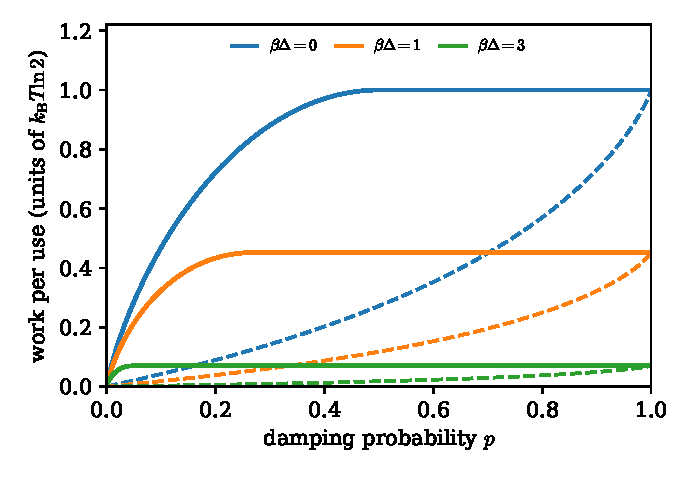
\includegraphics[width=0.62\linewidth]{fig-damping.pdf}
\caption{Work per use of amplitude damping with probability $p$, in real time (solid) and in batch (dashed), at three values of $\beta\Delta$. The curves meet only at $p=0$ and at full reset, $p=1$. Beyond $p=1/(1+e^{\beta\Delta})$ the real-time cost equals the cost of a full reset.}
\label{sw:fig:damping}
\end{figure}

The real-time formula has a striking consequence. Maximizing $h(y)-\beta\Delta y/\ln 2$ over all $y$ gives $y=1/(1+e^{\beta\Delta})$ and the value $\log_2(1+e^{-\beta\Delta})$, which is the cost of a full reset. So once $p\ge1/(1+e^{\beta\Delta})$, a partial reset costs exactly as much as a full one in real time (Figure~\ref{sw:fig:damping}). In batch, the cost of a partial reset rises smoothly to that value and reaches it only at $p=1$.

\paragraph{A finite example.} At one point the real-time cost can be met by a small explicit device. Take $p=1/2$ and $\beta\Delta=\ln2$. Since $p\ge1/(1+e^{\beta\Delta})$, the real-time cost is that of a full reset, $\log_2(3/2)$ bits or about $0.585\,\Delta$ per use, and the device never has to recover anything. Before the first input it prepares one ground-state qubit of gap $\Delta$ per use, and in round $t$ it applies the conserving rotation $|10\rangle\mapsto(|10\rangle+|01\rangle)/\sqrt2$ to the input and the $t$-th prepared qubit. The preparation uses only ordinary thermal qubits. Pool the $n$ memory qubits, initially thermal, with $R$ reservoir qubits of the same gap, and let a battery qubit of gap $w\Delta$ start excited. The $k$-excitation shell of the pool has dimension $\binom{R+n}{k}$. Whenever $\binom{R}{k+w}\ge\binom{R+n}{k}$, one energy-conserving permutation moves the whole shell onto states with every memory in its ground state, the reservoir in shell $k+w$ and the battery lowered; the other shells are left alone. The ratio $\binom{R}{k+w}/\binom{R+n}{k}$ decreases in $k$, so the preparation fails exactly on an upper tail of $\mathrm{Bin}(R+n,1/3)$. Because it happens before any input, its failure probability bounds the error against every adaptive observer once, not once per round. After the last output each memory is swapped with a fresh thermal qubit of the same gap, which returns the controller exactly on every branch. Table~\ref{sw:tab:finite} gives exact values for $n=100$. With $R=n^2$ and $w=n\log_2(3/2)+O(\sqrt{\ln n})$ the error is at most $n^{-2}$ for $n\ge1000$, by Hoeffding's inequality. The preparation is one large nonlocal permutation, not an efficient circuit.

\begin{table}[t]
\centering
\begin{tabular}{rrrrr}
reservoir $R$ & qubits & work & per use & error at most\\\hline
2{,}000  & 2{,}208  & $118\Delta$ & $1.18\Delta$ & $0.00999$\\
10{,}000 & 10{,}208 & $70\Delta$  & $0.70\Delta$ & $0.00548$\\
50{,}000 & 50{,}208 & $63\Delta$  & $0.63\Delta$ & $0.00156$
\end{tabular}
\caption{Real-time amplitude damping with $p=1/2$ at $\beta\Delta=\ln2$, for $n=100$ uses; the asymptotic cost is $0.585\Delta$ per use. The qubit count includes the reservoir, 100 memories, 100 fresh thermal qubits for the final swaps, a 7-qubit round counter and the battery. The battery drops by the stated work with probability one minus the error and is otherwise untouched. Errors are exact binomial tails, rounded up.}
\label{sw:tab:finite}
\end{table}

\paragraph{A finite saving.} The same example shows the batch saving at a finite size. At $p=1/2$ and $\beta\Delta=\ln2$ the batch capacity is about $0.154\,\Delta$ per use, against $0.585\,\Delta$ in real time, but batch constructions approach it only slowly. Fix the error at $10^{-8}$, and allow the controller to lose at most $10^{-5}\Delta$ of free energy, the battery to end with at most $10^{-5}$ bits of entropy, and its mean energy to differ from the nominal level by at most $10^{-5}\Delta$. Every real-time implementation of $234$ uses then has nominal work above $132.109\,\Delta$. This is~\eqref{sw:eq:converse} with the estimate of Appendix~\ref{sw:app:invertible} at the input with excited population $16/25$, where $\|(\Phi^c)^{-1}\|_\diamond=3$, less the three budgets. Only product inputs are used, so the bound also holds under the batch error criterion. A batch implementation does better. It prepares $234$ pure environment qubits for $137\Delta$ and runs the conserving partial swap of the real-time device. Before releasing the outputs it swaps the used environment into one of $32$ fresh thermal copies, chosen by a thermal five-qubit register, and then locates it again from the outputs, a position decoder as in~\cite[Sec.~7]{FBB21}. This purifies the register and returns $5\Delta$, so the nominal work is $137\Delta-5\Delta=132\Delta$, with error below $8.71\times10^{-9}$. At $256$ uses the same construction prepares the environments for $150\Delta$ and returns $11\Delta$ from $2^{11}$ positions: nominal work $139\Delta$ against a real-time bound of $144.53\Delta$, a saving above $5.5\Delta$. The saving needs the error: at zero error, the estimate of Appendix~\ref{sw:app:invertible} applied to the whole block gives a batch device the same bound as real time, as in the exact row of Theorem~\ref{sw:thm:werner}. The reservoirs that run the preparation and the refund are astronomically large, so this certifies that waiting saves work at a definite finite size, not that the saving is practical.

\subsection{The Werner--Holevo channel}\label{sw:sec:werner}

The Werner--Holevo channel $W(\rho)=(\Tr(\rho)\,I-\rho^T)/2$ on a qutrit is the standard example of a unital channel that is not a mixture of unitaries~\cite{LandauStreater93}. It is not even factorizable~\cite[Ex.~3.1]{HaagerupMusat11}, so it is not a limit of noisy operations. Its Choi state is the normalized projector onto the antisymmetric subspace of two qutrits. The isometry
\[
V|i\rangle=\tfrac{1}{\sqrt2}\sum_{j,k}\epsilon_{ijk}\,|j\rangle|k\rangle
\]
is a Stinespring dilation in which output and environment play symmetric roles, so $W$ is its own complementary channel. And $W$ is invertible, with $W^{-1}(Y)=\Tr(Y)\,I-2Y^T$.

\begin{proof}[Proof of Theorem~\ref{sw:thm:werner}]
\emph{Real time.} By Lemma~\ref{sw:lem:invertible}, $s_\rho(W)=S(W(\rho))$, which is at most $\log_2 3$ and equals it at $\rho=I/3$; so $\Trt(W)=\log_23$. Every exact real-time round on half of a maximally entangled pair adds exactly $\log_2 3$ bits of entropy to the device, whatever the device did before, and Lemma~\ref{sw:lem:accounting} gives $w\ge n\log_23$. With an information battery, a device that applies $V$ with one pure qutrit of the battery per round, and swaps the used qutrit into a thermal cell, attains this. At error $\varepsilon$ the same argument, run through the bounded inverse and continuity of conditional entropy on the nine-dimensional system $QO$, gives
\[
w\ \ge\ \sum_{t=1}^n\bigl[\log_2 3-g_9\bigl(\min\{1,10\sqrt{\varepsilon}\}\bigr)\bigr]_+,\qquad g_D(t)=2t\log_2 D+(1+t)\,h\bigl(t/(1+t)\bigr),
\]
which is $n\log_2 3-O(\log n)$ at $\varepsilon=n^{-2}$.

\emph{Batch.} The batch rate is zero by the theorem of Faist, Berta and Brand\~ao, since $\Tcap(W)=0$ for a unital channel at zero Hamiltonian~\cite{FBB21}. In the proof of their thermal-operation construction~\cite[Thm.~7.1]{FBB21}, the error at a fixed typicality tolerance $\delta$ is $\mathrm{poly}(n)\,e^{-n\eta/2}$, with an exponent $\eta=\eta(\delta)>0$ that tends to zero with $\delta$ (their Eqs.~(7.30), (7.36) and~(7.39)), and the work per copy tends to the capacity as $n\to\infty$ and then $\delta\to0$. At each fixed $\delta$ the error is below $n^{-2}$ for all large $n$, so letting $\delta$ step down to zero slowly enough, each step taken only once $n$ exceeds the threshold for the new value, gives work $o(n)$ at error $n^{-2}$. For exact batch implementation, the joint output-reference state must lie in the support of the $n$-fold antisymmetric projector, on which the partial trace acts as the invertible map $W^{\otimes n}$. The argument of Lemma~\ref{sw:lem:invertible} then forces $w\ge n\log_23$, attained by the same pure qutrits.
\end{proof}

No exact implementation can end with a sharp mechanical battery: each exact round triples the rank of the device, so if the controller returns, a battery that starts pure must end with rank at least $3^n$. This is why the exact entries of Theorem~\ref{sw:thm:werner} are stated for free energy.

The bound in the real-time part is measurable. Let $\delta$ be the average probability that the output and the reference of a round fail a two-outcome test for the antisymmetric subspace. Any real-time implementation, of any size and with any memory, then draws at least $n[\log_2 3-g_9(\min\{1,10\sqrt{\delta}\})]_+$ bits of free energy (Appendix~\ref{sw:app:werner}). We return to this in Section~\ref{sw:sec:discussion}.

The zero-error obstruction of Theorem~\ref{sw:thm:werner} holds for every extreme channel. A channel is extreme in the convex set of channels when the products $A_i^*A_j$ of its minimal Kraus operators are linearly independent~\cite{Choi75}; Werner--Holevo and amplitude damping with $0<p<1$ are examples.

\begin{proposition}[At zero error, waiting saves nothing for extreme channels]\label{sw:prop:extreme}
Let $\Phi$ be extreme with complementary channel $\Phi^c$, and let
\[
a_\beta(\Phi)=\max_\rho\Bigl[S(\Phi^c(\rho))+\tfrac{\beta}{\ln2}\Tr H\bigl(\Phi(\rho)-\rho\bigr)\Bigr].
\]
Every implementation of $n$ uses with zero error, in batch or in real time, draws at least $n\,a_\beta(\Phi)-o(n)$ bits of free energy from its battery and controller. For extreme channels $a_\beta(\Phi)=\Trt(\Phi)$, so at zero error a batch device pays the full real-time rate.
\end{proposition}

The proof is in Appendix~\ref{sw:app:extreme}: extremality makes the branches of any exact implementation orthogonal, so the device's entropy rises by exactly the entropy of the complementary output, whatever its initial state.

For amplitude damping at $p=1/2$ and $\beta\Delta=\ln2$, the asymptotic separation between $0.585\,\Delta$ per use in real time and the batch capacity $0.154\,\Delta$ therefore exists only because some error is tolerated. The finite constructions of Section~\ref{sw:sec:classical} certify smaller savings, at their stated block sizes and error budgets.

\subsection{What is free}\label{sw:sec:free}

A \emph{thermal operation} at $(H,\beta)$ is a channel $\rho\mapsto\Tr_BU(\rho\otimes\gamma_B)U^*$, where the bath $B$ (not the battery of Section~\ref{sw:sec:setting}) is finite-dimensional with an arbitrary Hamiltonian $H_B$, $\gamma_B$ is its Gibbs state at the same $\beta$, and $U$ commutes exactly with $H\otimes I+I\otimes H_B$~\cite{Janzing00,HorodeckiOppenheim13,Brandao13,vomEnde22,LieEtAl26}. We impose no large-bath conditions. The set is not closed~\cite{vomEnde22}, and by a limit of thermal operations we mean a point of its closure. \emph{Enhanced thermal operations} are the time-covariant channels that preserve $\gamma$~\cite{Cwiklinski15}.

Which processes are free? We call a process \emph{free in batch} (\emph{in real time}) if its optimal batch (real-time) work rate is zero, at vanishing error. Thermal operations, energy-conserving unitaries with a Gibbs bath, are the standard model of free dynamics~\cite{Janzing00,HorodeckiOppenheim13,Brandao13}. They preserve the Gibbs state and commute with time evolution~\cite{Lostaglio15}. Gibbs-preserving maps~\cite{Janzing00,FDOR15,FR18} are strictly more powerful: they can even create coherence between energy levels~\cite{FOR15}. The time-covariant ones, called enhanced thermal operations~\cite{Cwiklinski15}, coincide with the closure of the thermal operations for a qubit~\cite{Cwiklinski15,vomEnde22}, but not for a qutrit~\cite{Cwiklinski15,DingFengHu21}. By the theorem of Faist, Berta and Brand\~ao, a time-covariant process is free in batch exactly when it is an enhanced thermal operation (see below). In real time the answer is the thermal operations.

\begin{theorem}[What is free in real time]\label{sw:thm:free}
Let $\Phi$ be any channel on a system with Hamiltonian $H$, at any temperature. Then $\Trt(\Phi)=0$ if and only if $\Phi$ lies in the closure of the thermal operations.
\end{theorem}

Lie, Son, Boes, Ng and Wilming showed that a channel that fixes the Gibbs state is a thermal operation exactly when some dilation, with no energy conservation or thermal bath assumed, also leaves its environment unchanged when the input is the Gibbs state; energy conservation, a thermal bath and time covariance then follow~\cite[Prop.~4]{LieEtAl26}. Theorem~\ref{sw:thm:free} is a robust, work-cost form of their criterion. As in their exact case, zero cost forces time covariance and only the Gibbs input matters; here the bounds do not depend on the size of the bath, and this is what characterizes the closure.

So the enhanced thermal operations that are not limits of thermal operations are exactly the time-covariant processes that are free in batch but cost work in real time. This set is known to be nonempty. At zero Hamiltonian it contains the Werner--Holevo channel, which is not factorizable~\cite[Ex.~3.1]{HaagerupMusat11} and which Faist, Oppenheim and Renner cite as a unital map that is not a thermal operation~\cite{FOR15}, and for an equally spaced qutrit a channel of Ding, Ding and Hu~\cite{DingFengHu21}. We price both: $\log_23$ bits per use for the first (Theorem~\ref{sw:thm:werner}), and an explicit positive cost, at every gap ratio and temperature, for a family that contains the second (Proposition~\ref{sw:prop:qutrit}). For that family a single input state already separates the channel from every limit of thermal operations, with no assumption on the bath; Ding, Ding and Hu proved this for equally spaced levels, under assumptions on the bath and the temperature.

\paragraph{Batch.} For time-covariant $\Phi$ the batch cost is $\Tcap(\Phi)=\max_\rho[D(\Phi(\rho)\|\gamma)-D(\rho\|\gamma)]$, in relative-entropy form. The value at $\rho=\gamma$ is $D(\Phi(\gamma)\|\gamma)\ge0$, and by monotonicity of relative entropy every value is at most zero when $\Phi(\gamma)=\gamma$. So $\Tcap(\Phi)=0$ exactly when $\Phi$ is an enhanced thermal operation, and by the theorem of Faist, Berta and Brand\~ao such a process can be run in batch at vanishing work per use~\cite{FBB21}. This is a direct consequence of their work; we record it only for contrast. Faist, Oppenheim and Renner ask whether thermal operations aided by a time reference can do everything Gibbs-preserving maps can~\cite{FOR15}, and Tajima and Takagi showed that for some Gibbs-preserving maps no finite amount of coherence suffices~\cite{TajimaTakagi25}. For a device that carries its own phase reference and must return it, a Gibbs-preserving channel is free in batch exactly when its energy change lies in the span of the products of its Kraus operators; some non-covariant Gibbs-preserving channels are free and others cost work (Appendix~\ref{app:batch}).

\paragraph{Real time: thermal operations are free.} Let $\Phi$ be a thermal operation with bath $(H_B,\gamma_B)$. Its dilation is an exact extension in Definition~\ref{sw:def:rtcost}, with the bath purifier as $F$. Energy conservation and the Gibbs identity give, for every input,
\[
s_\rho(\Phi)+\tfrac{\beta}{\ln2}\Tr H\bigl(\Phi(\rho)-\rho\bigr)\ \le\ -D\bigl(\Gamma(\rho)\,\big\|\,\gamma_B\bigr)\ \le\ 0,
\]
where $\Gamma(\rho)$ is the bath output. So $\Trt(\Phi)=0$. If $\Phi$ is only a limit of thermal operations $\Phi_k$, the dilation of $\Phi_k$ is a feasible extension for $\Phi$ at error $\varepsilon$ once $\Phi_k$ is $\varepsilon$-close to $\Phi$, so the same bound holds for $s_{\rho,\varepsilon}(\Phi)$ up to an energy correction of order $\beta\varepsilon\,\mathrm{span}(H)$. Letting $\varepsilon\to0$, every limit of thermal operations has zero real-time cost as well. Operationally this is the obvious statement that a device using one fresh thermal bath per round runs a thermal operation in real time at no cost.

\paragraph{Real time: only thermal operations are free.} The converse is the substance of Theorem~\ref{sw:thm:free}. For baths of bounded size it follows from compactness and the exact characterization of Lie et al.~\cite{LieEtAl26}, but a small real-time cost may be achieved only with baths of unbounded size and arbitrarily small eigenvalues. We prove it in four steps (Appendix~\ref{sw:app:zero-set}).
\begin{enumerate}[label=(\roman*)]
\item Since $\Trt(\Phi)\ge D(\Phi(\gamma)\|\gamma)$, zero cost forces $\Phi(\gamma)=\gamma$. It also supplies dilations whose \emph{Gibbs defect} $G=D\bigl(U(\gamma\otimes\tau)U^*\,\big\|\,\gamma\otimes\omega\bigr)$ tends to zero, where $\omega$ is the bath output on input $\gamma$. The defect is the relative entropy between the joint output and the product of the Gibbs state with the bath output; it vanishes exactly for the equilibrating dilations of Lie et al., up to a unitary on the bath.
\item A small Gibbs defect forces time covariance. This is a robust form of Proposition~4 of~\cite{LieEtAl26}: the dilation nearly commutes with $(\gamma\otimes\tau)^{iz}$, the time evolution of $H+H_B$ with $H_B=-\beta^{-1}\ln\tau$, with a bound that involves neither the bath dimension nor its smallest eigenvalue.
\item A replacement theorem turns any dilation of a time-covariant channel with small defect $G$ into a finite thermal operation within $c_{H,\beta}\,G^{1/(6\max\{1,r\})}$ in diamond norm, where $r$ is the number of rationally independent energy gaps of $H$. The new thermal operation generally has a different bath.
\item Irrational energy gaps are approximated by commensurate ones with the same integer labels, and a finite thermal lattice absorbs the difference so that the original Hamiltonian is conserved exactly. This handles the accidental gap coincidences at which thermal operations depend discontinuously on $H$~\cite[Sec.~III]{vomEnde22}. No external phase reference is used.
\end{enumerate}
As in the exact criterion of Lie et al., only the Gibbs input matters: $\Phi$ is a limit of thermal operations exactly when $\Phi(\gamma)=\gamma$ and the real-time entropy cost at the Gibbs input vanishes. Lie et al.\ also observe that an enhanced thermal operation outside the thermal operations must change its environment even at the Gibbs input, so its environment must hold non-equilibrium free energy, which may be depleted~\cite{LieEtAl26}. The real-time entropy cost $s_\gamma(\Phi)$ is the least such change, and in real time it is paid in work.

Two remarks on the controller. The controller acts as a catalyst that is returned only at the end and may be correlated with past outputs; it does not enlarge the free set, because those correlations only add to the cost in Lemma~\ref{sw:lem:accounting} and its free energy must return up to $o(n)$, which also excludes the embezzlement that a catalyst returned only approximately would otherwise allow~\cite{FOR15}. And since the lower bound of Section~\ref{sw:sec:law} holds for any controller, Theorem~\ref{sw:thm:free} bears on the time-reference question of Faist, Oppenheim and Renner~\cite{FOR15}: a phase reference that the device must return, up to $o(n)$ free energy, cannot make a non-covariant Gibbs-preserving map free in real time. A reference that is used up and paid for is not covered.

\paragraph{A clock that returns cannot help.} If the controller returns exactly, as in our constructions of time-covariant channels, and the battery is stationary, a non-covariant channel cannot be run at vanishing error, whatever work is spent~\cite{MarvianSpekkens19,LostaglioMuller19}. The following proposition makes this quantitative.

\begin{proposition}[A returning clock]\label{sw:prop:clock}
Suppose the controller returns exactly to $\alpha_C$, independent of all other systems, and the battery is stationary. Let $J_\Phi$ be the normalized Choi state of $\Phi$ and $G=H_O-H_I^T$, where $H_I=H_O=H$ act on the input and output. Then, in real time or in batch and whatever work is drawn, every implementation of $n$ uses of $\Phi$ has error at least
\[
\tfrac14\sup_t\bigl\|J_\Phi-e^{-\mathrm itG}J_\Phi e^{\mathrm itG}\bigr\|_1,
\]
which is positive exactly when $\Phi$ is not time-covariant. For the Hadamard gate on a qubit with $H=E|1\rangle\langle1|$ the error is at least $1-2^{-n}\binom{n}{\lfloor n/2\rfloor}$, which tends to one.
\end{proposition}

\begin{proof}
Fix an observer whose inputs, together with the systems it keeps, are invariant under time evolution; the initial reservoir states are invariant too, and so is the battery's, because it is stationary. Composing every operation of the device, including its final clean-up, and tracing out everything except the controller and a set $Y$ of systems we keep, gives a channel $\Lambda$ from $C$ to $CY$ that commutes with time evolution. Exact return means $\Lambda(\alpha)=\alpha\otimes\rho$. Write $x_t$ for a state evolved for time $t$. Covariance gives $\Lambda(\alpha_t)=\alpha_t\otimes\rho_t$, and since fidelity does not decrease under $\Lambda$ and is multiplicative on products, $f(\alpha,\alpha_t)\le f(\alpha,\alpha_t)f(\rho,\rho_t)$. For small $t$ the fidelity $f(\alpha,\alpha_t)$ is positive, so $\rho_t=\rho$, and by the group law this holds for every $t$. So the final state of everything we keep is invariant in time: a controller cannot pass on asymmetry and keep it, which is the no-broadcasting theorem for asymmetry~\cite{MarvianSpekkens19,LostaglioMuller19}.

For the first bound, let the observer send half of a maximally entangled state in the first round, and $|0\rangle$ in every later round, and keep the other half as a reference with Hamiltonian $-H^T$, so that the pair is invariant. The first output and the reference end in a state $J'$ that commutes with $G$, so $\|J_\Phi-e^{-\mathrm itG}J_\Phi e^{\mathrm itG}\|_1\le2\|J_\Phi-J'\|_1$ for every $t$, and the observer distinguishes $J'$ from $J_\Phi$ with advantage $\tfrac12\|J_\Phi-J'\|_1$. For the Hadamard gate, send $|0\rangle$ in every round. The outputs end in a state that commutes with the total energy, while the ideal output $|+\rangle^{\otimes n}$ has weight $2^{-n}\binom nk$ in the sector with $k$ excitations. So the real output passes the test for $|+\rangle^{\otimes n}$ with probability at most $\max_k2^{-n}\binom nk$, and the ideal one with probability one.
\end{proof}

The battery must be stationary. A battery in a broad superposition of energy levels is a phase reference of its own, and the device may spend it while the controller returns exactly. Let the battery be a ladder with spacing $E$, prepared in a sine-shaped wave packet on $L$ consecutive levels with $n+1$ empty levels on each side, and let each use apply the Hadamard gate to every pair $\{|0\rangle|q\rangle,|1\rangle|q-1\rangle\}$ of equal total energy, and the identity on the two unpaired states at the edges. This unitary conserves energy. Because the packet barely changes when it is shifted by one level, each use acts as the Hadamard gate up to $\pi/(\sqrt2(L+1))$ in strategy distance, whatever the observer does. With $L=n^3$ and a trivial controller, $n$ uses have error $O(n^{-2})$, while the battery's entropy changes by at most $\log_2(L+2n+2)=o(n)$. The battery's coherence is spent, not broadcast, so this is consistent with the no-broadcasting theorem; it shows that every initial store of asymmetry, a coherent work store included, must be counted as part of the controller.

\paragraph{A clock that returns approximately.} Theorem~\ref{sw:thm:clock} relaxes the return condition. A controller \emph{returns approximately} if, uniformly over observers, its final joint state with all other systems is within $\eta_n\to0$ in trace distance of $\alpha_C$ tensored with their final state, and its mean energy and its entropy change by $o(n)$. This is the return condition of our lower bounds, with closeness of the joint state added. Trace-distance closeness alone would not suffice: a broad reference can hand over energy of order $n$ while staying close to its initial state, and would then act as a second battery. The controller may start with any declared amount of phase reference.

\begin{theorem}[A clock that returns approximately]\label{sw:thm:clock}
Let $\Phi$ be any channel. Suppose the controller need only return approximately: its final joint state with everything else is close to its initial state tensored with the rest, and its mean energy and its entropy change by $o(n)$. Then the optimal real-time work per use at vanishing error is $\kB T\ln2\,\Trt(\Phi)$, with deterministic work. For a unitary $U$ it is exactly the largest eigenvalue of $U^*HU-H$, and the battery reaches its target on every branch. If $U$ is not time-covariant, the heat baths of any such implementation with deterministic work must have a total energy range that grows faster than $n$.
\end{theorem}

Faist, Berta and Brand\~ao leave open whether thermal operations can implement every i.i.d.\ channel that is not time-covariant at its thermodynamic capacity, and expect this to need a very large amount of coherence, as the reverse Shannon theorem needs embezzling states~\cite{FBB19},~\cite[Sec.~9]{FBB21}. Theorem~\ref{sw:thm:clock} settles the real-time analogue of this question: a clock that returns approximately runs every channel at the optimal real-time rate, and the coherence it needs is indeed large. In batch, a clock that must return in the same sense, which rules out embezzlement, cannot always reach the capacity: for qubit dephasing in the $X$ basis, batch costs as much as real time, more than the capacity, and the batch cost of every channel with a returned clock is given in Appendix~\ref{app:batch}. The coherence is invested, not consumed. The operating work is the same formula, while for a gate the clock pays in capital~\cite{ChiribellaYangRenner21,TSS20} and the baths in energy range, and the controller's energy comes back only on average, not branch by branch (Appendix~\ref{app:batch}). Channels that are not gates can need far less: a Gibbs-preserving qubit channel that only creates coherence runs in batch at its capacity, zero, with a clock whose energy spreads like $\sqrt n$ (Appendix~\ref{app:batch}).

The lower half of Theorem~\ref{sw:thm:clock} is the bound of Section~\ref{sw:sec:law}, which uses neither time covariance nor exact return. The construction (Appendix~\ref{sw:app:clock}) rests on one primitive. Let $D=U^*HU-H$, $w$ its largest eigenvalue and $B=wI-D\ge0$. A thermal qubit with a large gap $M$ can absorb the energy $B$ by a rare excitation: a rotation between the payload and this qubit, by the angle whose sine is $\sqrt{B/M}$, changes the payload channel by only $O(\|B\|/M)$, yet the qubit takes up exactly the input-dependent part of the energy change, on average. What remains is the constant $w$, which a sharp battery supplies. Lifting the whole contact with a phase reference makes it conserve energy exactly, and the reference's energy then drifts by $O(1/M)$ as an operator, whatever the input. For the Hadamard gate on a qubit with $H=E|1\rangle\langle1|$, this gives work exactly $nE/\sqrt2$, with error and return error $O(n^{-3})$. For a general channel the same primitive is applied to a dilation whose bath carries the Hamiltonian $-\beta^{-1}\ln\zeta$, with $\zeta$ the bath state at the worst input. This turns the bath's entropy into energy, so one operator inequality handles the entropy and energy terms together. The bath copies are prepared in their source state, and everything used to prepare them is returned, by the finite-source module of Appendix~\ref{app:module}, applied with one slot.

The energy-conserving lift and the reusable reference go back to {\AA}berg~\cite{Aberg14}. Repaying a reference's drift with work is due to Korzekwa, Lostaglio, Oppenheim and Jennings~\cite{KLOJ16}, and forming coherent sources at their free-energy cost to~\cite{Brandao13,KLOJ16}. The rare-excitation primitive and the work rate for every channel appear to be new. The bound on the baths' range is an argument of Wigner--Araki--Yanase type, of the kind that bounds the energy and coherence a reference needs to implement a gate~\cite{ChiribellaYangRenner21,TSS20}; what is new is that, with deterministic work and a controller that returns, it falls on the heat baths. Faist, Berta and Brand\~ao already observed that for such channels the environment must coherently compensate the energy differences between inputs~\cite{FBB19}; the bound makes this quantitative.

\paragraph{The clock is expensive.} Theorem~\ref{sw:thm:clock} makes the operating work the formula, but the clock is not cheap. Unlike a circuit acting on one register, whose energy requirement need not grow with its depth~\cite{ChiribellaYangRenner21}, $n$ uses on fresh systems call for $n$ times the asymmetry. In Appendix~\ref{app:batch} we show that, for a gate, its initial free energy must grow at least like $n/(\varepsilon+\eta)$, where $\eta$ is the return error, a quantitative form of the trade-off between disturbing a reference and the asymmetry it can impart~\cite{MarvianSpekkens19}, that the range of its baths and the strength of their interactions must grow at least like $n/\sqrt\varepsilon$, and that its energy comes back only on average, through a lottery of rare large transfers.

At zero Hamiltonian a thermal operation is a mixture of noisy operations, unitaries acting with a maximally mixed bath~\cite{HHO03}. Lie et al.\ note that these mixtures are the strongly factorizable channels, and show that these are exactly the unital channels with an equilibrating dilation~\cite[Eq.~(14)]{LieEtAl26}, and their closure is the closure of the channels that factor through a finite-dimensional algebra with a faithful trace~\cite{MullerHermesPerry,Douglas26closed}. Thus at zero Hamiltonian Theorem~\ref{sw:thm:free} identifies real-time freeness with the closure of finite-dimensional factorizability, as in our earlier work~\cite{Memory}. The closure is needed: a channel can be a limit of finitely factorizable channels without factoring through any finite-dimensional algebra~\cite{MusatRordam}.

\paragraph{The gap.} For a qubit, enhanced thermal operations coincide with the closure of the thermal operations~\cite{Cwiklinski15},~\cite[Thm.~10]{vomEnde22}. For a qutrit they do not, already for state transitions: exactly~\cite{Cwiklinski15} and approximately~\cite{DingFengHu21}. By Theorem~\ref{sw:thm:free}, the difference is exactly the set of time-covariant processes that are free in batch but cost work in real time. At zero Hamiltonian it contains the Werner--Holevo channel, at a cost of $\log_2 3$ bits per use. At nonzero Hamiltonian it contains the following qutrit channels.

\begin{proposition}[A Gibbs-preserving process that is not free in real time]\label{sw:prop:qutrit}
Let $H=\mathrm{diag}(0,E_1,E_2)$ with $0<E_1<E_2$, let $\lambda=e^{-\beta E_2}$, and let $\Phi$ have Kraus operators $\mathrm{diag}(\sqrt{1-\lambda},1,0)$, $\sqrt\lambda\,|2\rangle\langle0|$ and $|0\rangle\langle2|$. Then $\Phi$ is an enhanced thermal operation, so $\Tcap(\Phi)=0$, but
\[
\Trt(\Phi)\ \ge\ g_1\log_2\frac{1}{1-g_2}\ >\ 0,
\]
where $(g_0,g_1,g_2)$ are the Gibbs populations. Moreover, for the input $\psi_0=(|0\rangle+|1\rangle)/\sqrt2$ and every limit of thermal operations $\Theta$,
\[
\tfrac12\bigl\|\Theta(\psi_0)-\Phi(\psi_0)\bigr\|_1\ \ge\ \delta(\lambda)=\frac{(1-\lambda)\Delta_\lambda^2}{4(1-\lambda)\Delta_\lambda+2\lambda\bigl(1+2\sqrt{1-\lambda}\bigr)},\qquad\Delta_\lambda=\sqrt{1-\lambda}-(1-\lambda)>0.
\]
In particular $\Phi$ is at half diamond distance at least $\max\{\delta(\lambda),u^2/(2c^2)\}$ from the closure of the thermal operations, where $u=g_1g_2$ and $c=2+6u/\sqrt{1-\lambda}$.
\end{proposition}

The channel leaves level $1$ untouched, resets level $2$ to the ground state, and excites the ground state with probability $\lambda$, while keeping the coherence between levels $0$ and $1$ as large as positivity allows. The proof shows that the bath must end in orthogonal states after leaving level $1$ alone and after resetting level $2$. At the Gibbs input this forces correlations between bath and output worth at least $g_1\log_2\frac1{1-g_2}$ bits.

For equally spaced levels this is the enhanced thermal operation that Ding, Ding and Hu use (their Eq.~(11) with the transition matrix of their Eq.~(17)). It saturates the coherence bounds of~\cite{Cwiklinski15,Lostaglio15}. They proved that its output on $\psi_0$ cannot be approximated by any thermal operation acting on that input~\cite{DingFengHu21}, for equally spaced levels, bath degeneracies that grow with energy as in~\cite{HorodeckiOppenheim13}, and a range of temperatures. Proposition~\ref{sw:prop:qutrit} removes all three assumptions and bounds the trace distance explicitly. Their bound is stated for perturbations of transition probabilities, so the two constants are not directly comparable.

The single-input bound rests on a law for thermal operations that may be of independent interest (Lemma~\ref{sw:lem:coherence}). If a thermal operation moves the ground state to level $2$ with probability $T_{20}$, then $T_{20}\le\lambda$, and the coherence it keeps between levels $0$ and $1$ is at most $\frac12\bigl[1-\lambda+\sqrt{\lambda(\lambda-T_{20})}\bigr]$. The reason is that the bath can give up the energy $E_2$ only from states of total Gibbs weight at most $\lambda$. Moving the full probability $\lambda$ to level $2$ therefore forces an all-or-nothing transfer on those states, while $\Phi$ acts as if every state of the bath contributed the same partial amplitude $\sqrt\lambda$. With $T_{20}=\lambda$, $\Phi$ keeps the coherence $\sqrt{1-\lambda}/2$, above the bound by $\Delta_\lambda/2$.

\subsection{Undecidability}\label{sw:sec:undecidable}

Our last result concerns generalized dephasing channels, also called Schur multiplier channels: $\Phi(\rho)=M\circ\rho$, the entrywise product with a positive semidefinite matrix $M$ that has unit diagonal.

\begin{theorem}[Undecidability]\label{sw:thm:undecidable}
There is a dimension $d_0$ with the following property. For every $d\ge d_0$, every Hamiltonian on $\mathbb C^d$ that is diagonal in the dephasing basis and every temperature, no algorithm decides whether a generalized dephasing channel on $\mathbb C^d$ with cyclotomic entries is free in real time. The set of such channels that are free is not recursively enumerable.
\end{theorem}

By Theorem~\ref{sw:thm:free}, free in real time means a limit of thermal operations; on these channels the easy direction of Theorem~\ref{sw:thm:free} is enough, because the other direction is supplied by the zero-Hamiltonian closure theorem of our earlier preprint~\cite[Thm.~3.2(a)]{Memory} (Step~1 of the proof below). In batch the same question is trivial: a generalized dephasing channel preserves every energy population, hence the Gibbs state, so it is always free in batch. Our earlier work showed that the zero-Hamiltonian question is undecidable when the dimension may grow~\cite{Flagship}; Theorem~\ref{sw:thm:undecidable} settles the fixed-dimension question left open there.

On dephasing channels the Hamiltonian and the temperature drop out. Being free in real time becomes a question about which Gram matrices of unitaries finite-dimensional algebras can approximate, and that question is undecidable at a fixed size by the work of Fu, Miller and Slofstra.

\begin{proof}[Proof of Theorem~\ref{sw:thm:undecidable}]
\emph{Step 1: on dephasing channels, free means a limit of finitely factorizable channels.} Let $\Phi(\rho)=M\circ\rho$ be a generalized dephasing channel, and let the Hamiltonian be diagonal in the same basis. Then $\Phi$ preserves every energy population, so the energy term vanishes and $\Trt(\Phi)=\sup_\rho s_\rho(\Phi)$, the zero-Hamiltonian purity cost of our earlier work. That cost vanishes exactly when $\Phi$ is a limit of channels that factor through finite-dimensional algebras with a faithful trace~\cite[Thm.~3.2(a)]{Memory},~\cite{Douglas26closed}. For dephasing channels these are the limits of channels with $M_{ij}=\tau(u_j^*u_i)$ for unitaries $u_i$ in a finite-dimensional algebra $\mathcal N$ with faithful trace $\tau$~\cite{HaagerupMusat11,Musat25}. Each such channel is a thermal operation. Write $\mathcal N=\bigoplus_k M_{n_k}$ with $\tau=\sum_kw_k\tr_{n_k}$ (normalized traces), give the bath the Hamiltonian $H_B=\bigoplus_kE_kI_{n_k}$ with $e^{-\beta E_k}=w_k/n_k$, so that its Gibbs state is the density of $\tau$, and use $U=\sum_i|i\rangle\langle i|\otimes u_i$. This $U$ commutes with $H\otimes I+I\otimes H_B$, its bath starts in the Gibbs state, and it implements $\Phi$. (This is the dilation used for Schur multipliers in~\cite{HaagerupMusat11,LieEtAl26}, with the bath Hamiltonian read off from the trace as in~\cite{LieEtAl26}.) Conversely, every limit of thermal operations has zero real-time cost (Section~\ref{sw:sec:free}). So a dephasing channel is a limit of thermal operations exactly when it is a limit of finitely factorizable channels, at every temperature and for every Hamiltonian diagonal in its basis. This step does not use the hard direction of Theorem~\ref{sw:thm:free}; the direction it needs, from zero cost to a limit of finitely factorizable channels, is imported from~\cite[Thm.~3.2(a)]{Memory}.

\emph{Step 2: the reduction.}
\begin{enumerate}[label=(\alph*), leftmargin=*]
\item For a recursively enumerable but not recursive set $X$, Fu, Miller and Slofstra give a number $N$ of questions, eight answers, and a computable map from $n$ to finite lists of real tables with cyclotomic entries: if $n\in X$ none of them is a commuting-operator correlation, and if $n\notin X$ one of them is an approximately quantum synchronous correlation~\cite[Thm.~7.2]{FMS}. Exact tests discard every table that is not a synchronous correlation (Appendix~\ref{sw:app:fixeddim}).
\item Approximately quantum synchronous correlations are exactly those realized by projections in an ultrapower of the hyperfinite factor~\cite{KPS18}.
\item The construction of Musat and R{\o}rdam turns such projections into unitaries in the same algebra with a prescribed Gram matrix~\cite{MusatRordam}.
\item The corresponding dephasing channel on $\mathbb C^{d_0}$, $d_0=16N+1$ (the identity, the $8N$ symmetries $2p_j-1$ and the $8N$ unitaries $(2p_j-1+i)/\sqrt2$), is a limit of finitely factorizable channels exactly when its Gram matrix is a limit of finite-dimensional ones~\cite{Musat25}. Repeating indices embeds it in every dimension $d\ge d_0$.
\end{enumerate}
The entries lie in cyclotomic fields: the construction of Fu, Miller and Slofstra uses sines and cosines of rational multiples of $\pi$ and finite group-algebra coefficients~\cite[Sec.~7, Thm.~7.2]{FMS}, and the transfer to unitaries adds only $i$ and $\sqrt2$. The field grows with $n$; no fixed number field is claimed. So each channel is a finite, exact input. Appendix~\ref{sw:app:fixeddim} gives the reduction in full: the faithful Gram transfer, the exact filters on the tables, and the padding to larger dimensions. Program $n$ never halts exactly when some channel in its list is free; when it halts, no channel in the list is even factorizable. If the free channels were recursively enumerable, the non-halting programs would be too, which is impossible.\footnote{The reduction asks whether at least one channel in a finite list is free, so it is a disjunctive truth-table reduction from the complement of the halting problem rather than a many-one reduction. The dimension $d_0=16N+1$ is not explicit, because Fu, Miller and Slofstra do not give $N$ explicitly.}
\end{proof}


\subsection{Discussion}\label{sw:sec:discussion}

\paragraph{Order, not speed.} For protocols with a reversible quasistatic limit, the excess work due to finite speed vanishes as the protocol is slowed. The surcharge here does not: our rates allow devices of any size and any running time, so the gap between $\Trt$ and $\Tcap$ survives arbitrarily slow operation. It is a cost of order: an operation becomes more expensive, without being performed faster, because some of its outputs must become unavailable sooner.

\paragraph{A laboratory test.} The Werner--Holevo bound needs no knowledge of the device beyond our accounting: declared reservoirs, a mechanical battery and a controller that returns. Feed each round one half of a maximally entangled pair of qutrits, test the output and the kept half for the antisymmetric subspace, and record the average failure probability $\delta$. Every real-time implementation, of any size and with any memory, then draws at least $n[\log_2 3-g_9(\min\{1,10\sqrt\delta\})]_+$ bits of free energy from its battery and controller. With a mechanical battery whose entropy does not change and a returning controller, this free energy leaves as heat into the reservoirs (Lemma~\ref{sw:lem:accounting}). A qutrit platform that implements the channel round by round must therefore warm its environment by nearly $\kB T\ln 3$ per use, whereas a batch implementation need not, in principle. The correction term is weak: the bound is informative only for $\delta$ below about $2\times10^{-4}$, and within ten percent of $\log_2 3$ only near $\delta=10^{-6}$. Sharpening it, and turning it into a protocol with confidence intervals, is a separate task.

\paragraph{Processes with memory.} Our results concern repeated uses of one channel. A process whose later steps depend on earlier inputs is different: if an earlier output must leave before a later input arrives, the device has to keep a record correlated with an output it has already released, and erasing the part of that record that later outputs do not reveal costs work even when everything is classical. For agents whose memory is a function of the past, this is the online cost of~\cite{Thompson25}, and the modularity dissipation of classical computation, the loss of correlations with degrees of freedom that a local operation cannot act on, has the same form~\cite{BMC18}; agents that extract work efficiently must balance prediction against forgetting~\cite{Fiderer26}. Earlier, Still, Sivak, Bell and Crooks showed that in a system driven by a stochastic signal the average work dissipated at each change of the signal equals, in units of $\kB T$, the information its memory keeps about the signal that does not predict the signal's next value~\cite{Still12}; the constraint here is different, the loss of access to outputs at a prescribed release. Processes with several time steps that preserve thermal equilibrium have been characterized as the causally ordered thermal ones~\cite{Milz26}. The common principle is that the price of real time is the correlation a device must keep with outputs it has already released. For a repeated classical channel no such correlation is needed on inputs diagonal in its basis, and those inputs set its optimal cost (Theorem~\ref{sw:thm:classical}); for a quantum channel it can be forced (the term $m_\rho$); for a process with memory the task itself forces it.

\paragraph{Waiting a little.} For time-covariant channels, a device that may hold some outputs before releasing them sits between the two regimes. For each fixed tolerance $\delta>0$ there is a constant $C_\delta$ such that running blocks of length $C_\delta\log(n/\varepsilon)$ in batch, a delay that grows with the number of uses, comes within $\delta$ of the batch rate. In this construction, reaching the batch rate itself takes a delay that grows faster than $\log(n/\varepsilon)$, and the exact work--latency profile, including the cost at a fixed latency, is open (Section~\ref{to:sec:waiting}). For other channels with a returned clock, the batch endpoint is the single-letter cost of Appendix~\ref{app:batch}, which can exceed $\Tcap$.

\paragraph{Open problems.} Our constructions use reservoirs of astronomical size; efficient reservoirs, and an autonomous engine with a time-independent Hamiltonian, are open. For channels that are not time-covariant, the batch cost with a returned clock is a single-letter quantity (Appendix~\ref{app:batch}); whether it can be reached with modest reference capital is open. The constant $\delta(\lambda)$ in Proposition~\ref{sw:prop:qutrit} is not optimal. Thermal operations built from partial swaps come within about $0.10\lambda$ of $\Phi(\psi_0)$ at low temperature and $(1-\lambda)/2$ at high temperature, and numerical searches find nothing closer; the exact distance is open. Finally, $\Trt$ is defined by an optimization whose zero set is undecidable; computable bounds for typical channels would make the law practical.


\subsection{The construction}\label{sw:app:construction}

Except in the first subsection, whose statements hold for every channel and are used again in Appendix~\ref{sw:app:clock}, $\Phi$ is time-covariant. Throughout, $H$ and $\beta$ are fixed, entropies are in bits, and
\[
e_H(\rho)=\tfrac{\beta}{\ln2}\Tr H\bigl(\Phi(\rho)-\rho\bigr)=\Tr\rho\,D_H,\qquad D_H=\tfrac{\beta}{\ln2}\bigl(\Phi^*(H)-H\bigr).
\]
An \emph{exact dilation} $\Dil=(U,\tau)$ is a finite unitary $U$ on the system and a bath $B$ of dimension $R$ in state $\tau$, with $\Phi(\rho)=\Tr_BU(\rho\otimes\tau)U^*$. Let $\Gamma(\rho)=\Tr_SU(\rho\otimes\tau)U^*$ be its bath output and $f_{\Dil}(\rho)=S(\Gamma(\rho))-S(\tau)$.

\subsubsection{One dilation for all inputs}

For each full-rank $\rho$, the real-time entropy cost is the infimum over exact dilations,
\begin{equation}\label{sw:eq:pointwise}
s_\rho(\Phi)=\inf_{\Dil} f_{\Dil}(\rho),
\end{equation}
by the pointwise smoothing identity (Lemma~\ref{sw:lem:smoothing}). An exact dilation is an exact extension, which gives $\le$. Conversely, an $\varepsilon$-feasible extension lifts to a dilation at diamond error $\varepsilon/\lambda_{\min}(\rho)$ with the same objective, and a repair that changes the objective by a quantity tending to zero, independently of the extension's size, makes it exact.

\begin{lemma}[Minimax]\label{sw:lem:minimax}
$\Trt(\Phi)=\inf_{\Dil}\max_\rho\bigl[f_{\Dil}(\rho)+e_H(\rho)\bigr]$, the infimum over finite exact dilations.
\end{lemma}

\begin{proof}
Write $F_{\Dil}=f_{\Dil}+e_H$. Each $F_{\Dil}$ is continuous and concave on the state space, and a finite convex combination $\sum_jp_jF_{\Dil_j}$ is realized by the direct sum of the $\Dil_j$ controlled by a flag register in state $\sum_jp_j|j\rangle\langle j|$; the flag's entropy cancels in $f$. Let $a=\sup_\rho\inf_{\Dil}F_{\Dil}(\rho)$, which equals $\Trt(\Phi)$ by~\eqref{sw:eq:pointwise}, and fix $\delta>0$. Each $\rho$ has a dilation with $F_{\Dil}(\rho)<a+\delta$, which persists on an open neighbourhood. By compactness, finitely many $F_1,\dots,F_N$ satisfy $\min_jF_j(\rho)<a+\delta$ for every $\rho$. The set $\{x\in\mathbb R^N:x_j\le F_j(\rho)\ \forall j\ \text{for some}\ \rho\}$ is closed, convex and closed downwards, and excludes $(a+\delta,\dots,a+\delta)$. A separating hyperplane has a normal with nonnegative coordinates, which we normalize to weights $p_j$; then $\max_\rho\sum_jp_jF_j(\rho)<a+\delta$, and the flagged direct sum realizes $\sum_jp_jF_j$. Restricting to full-rank inputs changes nothing, since $|f_{\Dil}(\rho)-S(\rho)|\le\log d$ uniformly in $\Dil$, so concavity controls $F_{\Dil}$ near the boundary uniformly.
\end{proof}

Fix a dilation $\Dil$ with $g:=\max_\rho[f_{\Dil}(\rho)+e_H(\rho)]\le\Trt(\Phi)+\eta$, and write $\sigma=S(\tau)$ and $v=g+\sigma=\max_\rho[S(\Gamma(\rho))+e_H(\rho)]$.

\subsubsection{A joint first-order inequality}

Let $\rho_*$ maximize $S(\Gamma(\rho))+e_H(\rho)$ and $\zeta=\Gamma(\rho_*)$. The support $\mathcal S$ of $\zeta$ contains the support of every $\Gamma(\rho)$: mixing in weight $s$ outside $\mathcal S$ would raise the entropy by order $-s\log s$ and change everything else by $O(s)$. Put $L_B=-\log_2\zeta$ on $\mathcal S$ and $0$ on $\mathcal S^\perp$. The directional derivative of the concave maximand at $\rho_*$ gives $\Tr\Gamma(\rho)L_B+e_H(\rho)\le v$ for every $\rho$, that is,
\begin{equation}\label{sw:eq:firstorder}
\Gamma^*(L_B)+D_H\ \le\ v\,I.
\end{equation}
For $t\ge0$ let $U_t=e^{t\beta H/2}Ue^{-t\beta H/2}$ (a similarity, not a physical operation) and
\[
A(t)=\Tr_B\bigl[(I\otimes\tau^{1/2})\,U_t^*\,(I\otimes2^{tL_B})\,U_t\,(I\otimes\tau^{1/2})\bigr].
\]
Then $A(0)=I$, $A(t)\ge0$, and $A'(0)=\ln2\,\Gamma^*(L_B)+\beta(\Phi^*(H)-H)\le v\ln2\,I$ by~\eqref{sw:eq:firstorder}. Since all dimensions are fixed, Taylor's theorem gives $C_0,t_0>0$ with
\begin{equation}\label{sw:eq:qt}
A(t)\ \le\ q(t)\,I,\qquad q(t)=\exp\bigl(t\,v\ln2+C_0t^2\bigr),\qquad0\le t\le t_0.
\end{equation}

\subsubsection{An energy register}

Let the additive group generated by the energy gaps of $H$ have rank $r$, with rationally independent generators $\omega_1,\dots,\omega_r$, and write $E_e=E_*+a_e\cdot\omega$ with integer vectors $a_e$ for the eigenvalues of $H$, with spectral projectors $P_e$. On the lattice $\mathbb Z^r$ let $T_u|b\rangle=|b+u\rangle$ and $H_L|b\rangle=(E_0+b\cdot\omega)|b\rangle$. Define
\[
\mathcal L(X)=\sum_{e,f}(P_e\otimes I)\,X\,(P_f\otimes I)\otimes T_{a_f-a_e}.
\]
Orthogonality of the $P_e$ and $T_uT_v=T_{u+v}$ make $\mathcal L$ a unital $*$-homomorphism, so $V=\mathcal L(U)$ is unitary. The term $P_eXP_f$ changes the system energy by $E_e-E_f$ and moves the lattice by $a_f-a_e$, so $V$ conserves $H+H_L$ exactly; the bath cells have zero Hamiltonian. With $Q(t)=e^{-t\beta H_L/2}$ one checks $Q(t)VQ(t)^{-1}=\mathcal L(U_t)$, and hence, averaging over a fresh bath cell,
\begin{equation}\label{sw:eq:effect}
\Tr_B\Bigl[(I\otimes\tau^{1/2})\,V^*\bigl(I\otimes2^{tL_B}\otimes e^{-t\beta H_L}\bigr)V\,(I\otimes\tau^{1/2})\Bigr]=Q(t)\,\mathcal L(A(t))\,Q(t)\ \le\ q(t)\,I\otimes e^{-t\beta H_L}.
\end{equation}
This is an operator inequality on system and lattice together, so it holds for every joint input, with any reference attached. Only a finite box of the lattice is used: with $A_{\max}=\max_e\|a_e\|_\infty$, the box $\|b\|_\infty\le2(n+1)A_{\max}$ contains every coordinate reachable in $n$ rounds from $b=0$, the lifted unitary is specified exactly on reachable columns, and it is completed to a unitary separately inside each total-energy eigenspace. The box has dimension polynomial in $n$. The register starts in $|0\rangle$, a sharp energy eigenstate of energy $E_0=O(n)$ chosen to make all energies nonnegative, and it is counted as part of the battery.

\subsubsection{Why the register does not disturb the channel}

Fourier transformation diagonalizes the lattice translations, and $|0\rangle$ has the uniform distribution on the torus generated by the gaps. In the fibre of a phase $\theta$, the lifted unitary acts as $D_\theta UD_\theta^*$, where $D_\theta$ is the corresponding energy phase on the system. Tracing out the register therefore averages the whole adaptive experiment, with every round conjugated by the same $D_\theta$. Time covariance, with continuity, makes $\Phi$ commute with every $D_\theta$, so every fibre runs $n$ ideal uses of $\Phi$ and so does the average. This is the only place where time covariance is used.

\subsubsection{The weighted projector}

Run $n$ rounds, each with the lifted unitary on a fresh cell $B_i$ and the same register, and keep the used cells until the end. Let $W_j(t)=\prod_{i\le j}2^{tL_{B_i}}\otimes e^{-t\beta H_L}$. Before round $j$ the fresh cell is independent of everything else; the old factors are positive and act on other systems; and the observer's operations act on neither the cells nor the register. So~\eqref{sw:eq:effect} multiplies the expectation of $W_j(t)$ by at most $q(t)$ per round, whatever the correlations between system, register, old cells and references, and
\begin{equation}\label{sw:eq:supermart}
\Tr\Bigl[\rho_{\mathrm{fin}}\prod_{i=1}^n2^{tL_{B_i}}\,e^{-t\beta(H_L-E_0)}\Bigr]\ \le\ q(t)^n.
\end{equation}
Let $P$ be the spectral projector, inside $\mathcal S^{\otimes n}$, of $\sum_iL_{B_i}-\beta(H_L-E_0)/\ln2$ for values at most $n(v+\gamma)$. By Markov's inequality and~\eqref{sw:eq:supermart} with $t=\gamma\ln2/(2C_0)$, its rejected weight is at most $\exp[-n(\gamma\ln2)^2/(4C_0)]$ for small $\gamma$, for every observer. For each lattice label $b$, $P$ admits only bath eigenstrings with $\prod_iz_{j_i}\ge2^{-n(v+\gamma)}e^{-\beta(E_L(b)-E_0)}$, where $z_j$ are the eigenvalues of $\zeta$; there are at most $2^{n(v+\gamma)}e^{\beta(E_L(b)-E_0)}$ of them. Hence $P$ commutes with $H_L$ and
\begin{equation}\label{sw:eq:gibbsvolume}
Z_P:=\Tr P\,e^{-\beta H_L}\ \le\ D_L\,e^{-\beta E_0}\,2^{n(v+\gamma)},
\end{equation}
where $D_L$ is the dimension of the register. Counting the rank of $P$ instead of its Gibbs weight would lose exactly the cancellation between entropy and energy.

\subsubsection{Forming the baths}

Take $\gamma=\gamma_n=n^{-1/4}$. The controller $C$ consists of the $n$ bath cells, a residue register of $2^{r_n}$ levels with $r_n=\lceil3n\gamma_n\rceil+4$, and an $(n+1)$-level clock, all with zero Hamiltonian, and starts maximally mixed of dimension $m_C=(n+1)R^n2^{r_n}$. A unitary on $C$ maps a flat state of rank $K=2^{\lceil n(\sigma+2\gamma_n)\rceil}$ to a state whose cell marginal is within $2e^{-c_\tau n\gamma_n^2}+2^{-n\gamma_n}$ of $\tau^{\otimes n}$: assign $\lfloor Kp_x\rfloor$ flat labels to each typical eigenstring $x$ of $\tau^{\otimes n}$, keeping distinct residue labels for its whole fibre. The flat state is formed thermally by a standard construction. Let $W_f=\beta^{-1}\ln(m_C/K)$, and take a reservoir with levels $jW_f$, $j=0,\dots,L_f$, of integer degeneracies $m_C^jK^{L_f-j}$, so that every level has the same Gibbs weight, and a work qubit with energies $0,W_f$ starting excited. Swapping the equal-energy, equal-dimension subspaces $C\otimes|1\rangle\otimes R_j$ and $\mathrm{ran}(\Pi)\otimes|0\rangle\otimes R_{j+1}$ for $j<L_f$ is energy-conserving, and produces the flat state with the qubit in its ground state with probability $1-1/(L_f+1)$, without any measurement. Every later gate on $C$ conserves energy because $H_C=0$; the clock runs the schedule, so the whole implementation is one fixed unitary.

\subsubsection{Paying the work}

\begin{lemma}[Gibbs-weight converter]\label{sw:lem:converter}
Let $X$ have Hamiltonian $H_X$, let $P,Q$ be projectors commuting with $H_X$, and let $w<\beta^{-1}\ln(Z_Q/Z_P)$, with $Z_P=\Tr Pe^{-\beta H_X}$. For every $\delta>0$ there is a finite thermal reservoir and an energy-conserving unitary on $X$, the reservoir and a two-level work register with energy gap $w$ such that, with an input-independent probability at least $1-\delta$, every state supported on $P$, with any reference, is sent into $Q$ while the work register moves from its initial to its final level. On the remaining branch, $P$-supported inputs are left unchanged.
\end{lemma}

\begin{proof}
Write the energies of $X$ and the value $w$ in an integer basis of the group they generate: $\epsilon_0+a\cdot\omega$ and $w=w_{\mathrm v}\cdot\omega$. Let $p_a,q_c$ be the ranks of $P,Q$ in energy sector $a,c$. Give reservoir tile $j\in J=\{\|j\|_\infty\le L\}$ the energy $E_R^0+j\cdot\omega$ and the integer degeneracy $g_j=\lfloor Ne^{\beta j\cdot\omega}\rfloor$, with $N$ so large that $(1-\theta)Ne^{\beta j\cdot\omega}\le g_j$ on $J$, where $s=\beta^{-1}\ln(Z_Q/Z_P)-w>0$ and $\theta\le(1-e^{-\beta s})/2$. All tiles have nearly equal Gibbs weight, so the interior $G=\{\|j\|_\infty\le L-D\}$, $D=\max\|a-w_{\mathrm v}-c\|_\infty$, carries probability at least $1-\delta$ for $L$ large. For each total coordinate $u$, let $I_u$ be the source subspace $P\otimes R_G\otimes|i\rangle$ with $a+j=u$ and $J_u$ the target $Q\otimes R_J\otimes|f\rangle$ with $c+k+w_{\mathrm v}=u$. Then
\[
\frac{\dim J_u}{\dim I_u}\ \ge\ \frac{(1-\theta)Ne^{\beta(u\cdot\omega-w)}\sum_cq_ce^{-\beta c\cdot\omega}}{Ne^{\beta u\cdot\omega}\sum_ap_ae^{-\beta a\cdot\omega}}=(1-\theta)e^{\beta s}>1.
\]
Swap each $I_u$ with an isometric image inside $J_u$ and act as the identity elsewhere. Distinct shells are orthogonal, so this is an energy-conserving unitary, and on the reservoir block $G$ it moves the whole $P$-subspace, coherently, into $Q$ with the work register in $|f\rangle$.
\end{proof}

After the last output, apply the converter with $X=C\otimes L$, $H_X=H_L$, the cut $P_X=P\otimes I_{\mathrm{residue}}\otimes I_{\mathrm{clock}}$ and the target $Q_X=I_C\otimes|0\rangle\langle0|_L$, for which $Z_{Q_X}=m_Ce^{-\beta E_0}$. By~\eqref{sw:eq:gibbsvolume} one can extract
\[
w_n=\beta^{-1}\ln\frac{m_Ce^{-\beta E_0}}{(n+1)2^{r_n}D_L\,e^{-\beta E_0}\,2^{n(v+\gamma_n)}}-s_n
\]
with any fixed slack $s_n>0$, and the register returns to $|0\rangle$. Finally swap $C$ with a fresh maximally mixed cell of the same dimension, which returns the controller exactly and independently. On the good branch the net work is
\begin{align*}
W_f-w_n&=\kB T\ln2\,\bigl[n(v+\gamma_n)-\lceil n(\sigma+2\gamma_n)\rceil+r_n+\log_2(n+1)+\log_2D_L\bigr]+s_n\\
&=n\kB T\ln2\,\bigl[g+O(n^{-1/4})\bigr].
\end{align*}
No delivered output is touched, and no part of the device is reset during the $n$ rounds.

\subsubsection{The battery and the error}

The battery is the formation qubit, the converter's work register and the lattice register. It starts in one sharp energy eigenstate, its dimension is polynomial in $n$, and all its energies are within $O(n)$. On the good branch it ends in a fixed sharp eigenstate. The failure probability $q_n$ is at most the sum of the formation failure, the typicality error, the rejected weight of $P$ and the converter failure; with $L_f$ and the converter's reservoir chosen so that the formation and converter failures are at most $n^{-8}$, $q_n=O(n^{-8})$. Because the energy range is $O(n)$, the mean work differs from the good-branch value by $O(nq_n)$, the battery's energy variance and entropy tend to zero, and the battery ends nearly independent of everything else. The complete error of the experiment is at most the formation and typicality errors, since everything after the last output acts on internal systems. Choosing dilations with $g\le\Trt(\Phi)+\eta$ and letting $\eta\to0$ slowly with $n$ gives one family with vanishing error and work rate $\Trt(\Phi)$, which proves the upper half of Theorem~\ref{sw:thm:law}.

\subsection{The fixed-error converse}\label{sw:app:fixed-error}

Let $T=CR$ be the controller together with all reservoirs, with Hamiltonian $H_T$, initially in the Gibbs state $\gamma_T$ and independent of a battery $B$ in a pure eigenvector $|b_i\rangle$ of $H_B$ with energy $E_i$. For a projector $P_B$ commuting with $H_B$ write
\[
b_\beta(P_B)=\tfrac{\beta E_i}{\ln2}+\log_2\Tr\bigl[P_Be^{-\beta H_B}\bigr]=\log_2\frac{\Tr P_Be^{-\beta H_B}}{e^{-\beta E_i}},
\]
the logarithm of the Gibbs weight of $P_B$ relative to the initial battery state. For a target eigenvector of energy $E_f$, $b_\beta=\beta(E_i-E_f)/\ln2$ is the work in bits. We bound the error against one observer: it feeds every round half of a fresh purification $\psi_\rho$ of a fixed input $\rho$, keeps the references, applies a fixed test to a random fraction of the rounds, and at the end measures the total energy of its systems. Since this observer is not adaptive, the bound holds for the complete error.

\subsubsection{\texorpdfstring{An input that commutes with $H$, and an affine price}{An input that commutes with H, and an affine price}}

Let $\bar s_\rho=s_\rho(\Phi)$. By~\eqref{sw:eq:pointwise}, $\rho\mapsto\bar s_\rho$ is an infimum of concave functions and hence concave. Time covariance makes it invariant under $\rho\mapsto e^{-iHt}\rho e^{iHt}$, and the energy term is invariant and affine. Averaging over the closure of the time translations therefore does not decrease $\bar s_\rho+e_H(\rho)$, so for every $\eta>0$ there is a full-rank $\rho$ with $[\rho,H]=0$ and $\bar s_\rho+e_H(\rho)\ge\Trt(\Phi)-\eta$. Fix it.

On states $\nu$ of $Y=QO$ with $\nu_Q=\rho^T$, let $g(\nu)=\inf S(QO|F)$ over extensions with $\nu_{QF}=\rho^T\otimes\sigma_F$. Mixing extensions with a flag makes $g$ convex, and its lower semicontinuous hull at $\chi_\rho$ is $\bar s_\rho$. By separation there is an affine $\ell\le g$ with $\ell(\chi_\rho)\ge\bar s_\rho-\zeta$, for any $\zeta>0$. Give the reference the bookkeeping Hamiltonian $-H^T$ and set $H_Y=-H^T\otimes I+I\otimes H$; then $\psi_\rho$ has $H_Y$-energy zero and, by covariance, $[\chi_\rho,H_Y]=0$. Averaging $\ell$ over the group generated by $H_Y$ keeps it affine, below $g$ and unchanged at $\chi_\rho$, and makes it depend only on the pinching of $\nu$ into the eigenspaces of $H_Y$. The device never acts on $Q$; the reference Hamiltonian is only used in the proof.

\subsubsection{An energy-preserving test}

In each eigenspace of $H_Y$, of dimension $m_j$, take the rank-one informationally complete measurement obtained by normalizing the frame $\{e_i\}\cup\{e_i+e_k\}\cup\{e_i+\mathrm ie_k\}_{i<k}$; together these give effects $\Lambda_x=|v_x\rangle\langle v_x|$, $L=\sum_jm_j^2\le d^4$ of them, from whose statistics a fixed linear map recovers the pinching of $\nu$. Fix $0<\gamma<1/4$ and let the observer apply in each round the instrument with Kraus operators $\sqrt{1-\gamma}\,I_Y$ (no test) and $\sqrt\gamma\,|u_j\rangle\langle v_x|$, where $u_j$ is a fixed unit vector in the same eigenspace as $v_x$. Every Kraus operator commutes with $H_Y$, and the instrument has a dilation that preserves $H_Y$ exactly, with outcome registers of zero energy.

Let $A_i$ be the round-$i$ system $Y_i$ together with its outcome. For every state of the device before round $i$, purified by a register $Z$ that the device does not touch, the fresh input makes $Q_iZ$ a product, so $S(Q_iO_i|Z)\ge g(\nu_{Q_iO_i})\ge\ell(\nu_{Q_iO_i})$. On a tested outcome $Y_i$ is pure and independent of $Z$. Hence $S(A_i|Z)\ge(1-\gamma)\,\ell(\nu_{Q_iO_i})$, and since the outcome statistics $q$ determine the pinching of $\nu$, the affine function $f(q)=(1-\gamma)\,\ell(\text{pinching recovered from }q_x/\gamma)$ is a min-tradeoff function for every input. No dimension of the device enters $f$.

\subsubsection{Entropy accumulation}

Let $q_*$ be the ideal distribution of outcomes, fix a slack $\zeta_s>0$, put $h=f(q_*)-\zeta_s$, and let $G$ be the event that the empirical score is at least $h$ and at most $2\gamma n$ rounds are tested. The ideal experiment fails $G$ with probability exponentially small in $n$, and
\[
|G|\le\sum_{k\le2\gamma n}\binom nk L^k\le2^{n\theta_\gamma},\qquad\theta_\gamma=h(2\gamma)+2\gamma\log_2L.
\]
With trivial Markov conditions and side information the thermofield purifier $E$ of $\gamma_T$, which nothing touches, the entropy accumulation theorem~\cite{DFR20} gives, whenever $p_G=\Pr(G)>0$ and $0<\delta<1$,
\begin{equation}\label{sw:eq:eat}
H_{\min}^\delta(A^n|E)_{|G}\ >\ nh-C_f\sqrt{n\,[1-2\log_2(\delta p_G)]},
\end{equation}
with a constant $C_f$ depending only on $d$, $L$ and the gradient of $f$.

\subsubsection{The energy cut}

Let $\Delta E=\Tr H(\Phi(\rho)-\rho)$ and $u>0$. The instrument preserves $H_Y$, so in the ideal experiment the total energy $H_{A^n}=\sum_iH_{Y_i}$ is a sum of independent bounded terms with mean $n\Delta E$, and the projector $P_A$ onto $H_{A^n}\ge n(\Delta E-u)$ rejects with probability exponentially small in $n$. It is applied only at the end, in the analysis. Let $p$ be the probability that $G$, $P_A$ and the battery projector $P_B$ all succeed in the real experiment; these projectors commute. If $e_n$ bounds the ideal rejection, then
\begin{equation}\label{sw:eq:p}
p\ \ge\ 1-\varepsilon_n-e_n-q,
\end{equation}
where $q$ is the probability, in this experiment, that the battery ends outside $P_B$. Finitely many small $n$ are absorbed into the constant $c$.

\subsubsection{A Gibbs-weighted cap}

\begin{lemma}\label{sw:lem:cap}
Let $\omega_{AEK}$ be pure with $(H_A+H_K-H_E)\,\omega=E_i\,\omega$. Suppose $H_A\ge L_E$ on the support of $\omega_A$, $\omega_E\le e^{-\beta H_E}/(pZ_E)$, and $\omega_K$ is supported in a subspace commuting with $H_K$ of Gibbs weight $Z_K$. Then for $0<s<1$
\[
H^s_{\min}(A|E)_\omega\ \le\ \log_2\frac{e^{\beta(E_i-L_E)}Z_K}{pZ_E}+2\log_2\frac2{1-s}.
\]
\end{lemma}

\begin{proof}
Because the global state lies in one eigenspace of the total charge, $\omega_{AE}$ commutes with $H_A-H_E$, and in the block paired with $K$-energy $k$ its rank is at most the dimension $d_k$ of the $K$-support at that energy. Let $a_0=(1-s)/(2Z_K)$ and let $\Pi$ project onto the eigenvectors of $\omega_{AE}$ whose eigenvalue in block $k$ is at least $a_0e^{-\beta k}$. The rejected trace is at most $a_0\sum_kd_ke^{-\beta k}=(1-s)/2$, and $\omega_{AE}\ge a_0\,e^{\beta(H_A-H_E-E_i)}\,\Pi$, all three operators commuting. Using $e^{-\beta H_A}\le e^{-\beta L_E}$ on the support and tracing out $A$,
\[
\Tr_A\Pi\ \le\ \frac{e^{\beta(E_i-L_E)}}{a_0}\,e^{\beta H_E/2}\omega_Ee^{\beta H_E/2}\ \le\ \frac{e^{\beta(E_i-L_E)}}{a_0pZ_E}\,I_E.
\]
Any subnormalized $\sigma_{AE}$ within purified distance $s$ of $\omega_{AE}$ has $\Tr\Pi\sigma\ge(1-s)/2$. If $\sigma_{AE}\le2^{-h_0}I_A\otimes\zeta_E$ for a state $\zeta_E$, then
\[
\tfrac{1-s}2\ \le\ \Tr\Pi\sigma_{AE}\ \le\ 2^{-h_0}\Tr\bigl[(\Tr_A\Pi)\,\zeta_E\bigr]\ \le\ 2^{-h_0}\,\frac{e^{\beta(E_i-L_E)}}{a_0pZ_E}.
\]
Substituting $a_0$ and optimizing over $\sigma_{AE}$ and $\zeta_E$ gives the bound.
\end{proof}

Apply the lemma to the normalized state after the three projections, with $A=A^n$, $E$ the thermofield purifier of $\gamma_T$ (so $H_E=H_T^T$, $Z_E=Z_T$), and $K$ the device, the battery and the observer's outcome registers. Energy conservation of every gate and of the observer's dilation gives the charge condition. The two copies of the accepted outcome string span a space of dimension $|G|$ at energy zero, so $Z_K=Z_T\,\Tr[P_Be^{-\beta H_B}]\,|G|$, and the reservoir's partition function cancels:
\begin{equation}\label{sw:eq:cap}
H^{1/2}_{\min}(A^n|E)_{\mathrm{proj}}\ \le\ b_\beta(P_B)-\tfrac{\beta n(\Delta E-u)}{\ln2}+n\theta_\gamma+\log_2\tfrac1p+4.
\end{equation}
No bound on the size or spectrum of the reservoir is used.

\subsubsection{\texorpdfstring{From the event $G$ to all three projections}{From the event G to all three projections}}

\begin{lemma}\label{sw:lem:postproj}
Let $\psi_{AEK}$ be pure and normalized, let $F=P\otimes P_K$ with projectors $P$ on $A$ and $P_K$ on $K$, let $r=\|F\psi\|^2>0$ and $\delta\le r/64$. Then $H^{1/2}_{\min}(A|E)_{F\psi/\sqrt r}\ge H^{\delta}_{\min}(A|E)_\psi+\log_2r$.
\end{lemma}

\begin{proof}
Take a near-optimal smoothing $\sigma_{AE}$ within purified distance $\delta$ of $\psi_{AE}$ and, by Uhlmann's theorem, a pure lift $\phi$ with $\|\psi-\phi\|\le\sqrt2\delta$. The filtered marginal $\sigma'_0=\Tr_KF\phi F$ satisfies $\sigma'_0\le P\sigma_{AE}P$, so if $\sigma_{AE}\le2^{-h_0}I_A\otimes\zeta_E$ then also $\sigma'_0\le2^{-h_0}I_A\otimes\zeta_E$; and $\Tr\sigma'_0\le r+\delta$. The state $\sigma'=\sigma'_0/(r+\delta)$ is subnormalized and has conditional min-entropy at least $h_0+\log_2(r+\delta)\ge h_0+\log_2r$. Its fidelity with $F\psi/\sqrt r$ is at least $(\sqrt r-\sqrt2\delta)/\sqrt{r+\delta}$, so their squared purified distance is at most $4\delta/r\le1/16$, and $\sigma'$ is an admissible smoothing at level $1/2$.
\end{proof}

\subsubsection{Assembly}

Combine~\eqref{sw:eq:eat} with $\delta=p/64$ and $p_G\ge p$, Lemma~\ref{sw:lem:postproj} with $r\ge p$, and~\eqref{sw:eq:cap}:
\[
b_\beta(P_B)\ >\ n\Bigl[h+\tfrac{\beta(\Delta E-u)}{\ln2}-\theta_\gamma\Bigr]-C_f\sqrt{n\,[13+4\log_2(1/p)]}-2\log_2\tfrac1p-4.
\]
Choose $\eta,\zeta,\gamma,\zeta_s,u$ so small that the bracket is at least $\Trt(\Phi)-\delta'/2$, where $\delta'$ is the gap of Theorem~\ref{sw:thm:fixed-error}; all these choices are made before $n$. If $b_\beta(P_B)\le n(\Trt(\Phi)-\delta')$ and $\log_2(1/p)\le an$ with $a=\min\{\delta'/16,\delta'^2/(256C_f^2)\}$, the right side exceeds the left for $n$ large, a contradiction. So $p<2^{-an}$, and~\eqref{sw:eq:p} gives $1-\varepsilon_n\le q+e_n+2^{-an}$, which is Theorem~\ref{sw:thm:fixed-error}.

\subsubsection{Which battery contracts are enough}

\begin{remark}[The battery must be counted]\label{sw:rem:counted}
Sharpness of energy alone is not enough. At zero Hamiltonian, a battery made of $n$ pure qutrits with zero energy can be swapped into the controller to run the exact Werner--Holevo implementation at zero energy cost. Its entropy then rises by $n\log_23$. In Theorem~\ref{sw:thm:fixed-error} this is paid through $b_\beta(P_B)$, which counts the dimension of the accepted battery subspace; a projector of rank $R_B$ at energies at least $E_i-W$ has $b_\beta\le\beta W/\ln2+\log_2R_B$.
\end{remark}

\begin{remark}[Mean work]\label{sw:rem:wernermean}
For the Werner--Holevo channel at zero Hamiltonian, form the pure bath cells with a thermal transducer that succeeds with a fixed probability $p<1$ and run an arbitrary implementation on failure. The error is at most $1-p$, the battery entropy is $h(p)$, and the mean work per use tends to $p\log_23<\Trt$. The theorem is not contradicted: the battery misses its target with probability $1-p$, and the work on the good branch is at the full rate.
\end{remark}

\subsection{What is free in real time}\label{sw:app:zero-set}

For a dilation $\Dil=(U,\tau)$ of a channel $\Psi$, let $\Omega=U(\gamma\otimes\tau)U^*$, $\omega=\Tr_S\Omega$, and define the \emph{Gibbs defect}
\[
G_{\Dil}=S(\omega)-S(\tau)+\tfrac{\beta}{\ln2}\Tr H\bigl(\Psi(\gamma)-\gamma\bigr)=f_{\Dil}(\gamma)+e_H^\Psi(\gamma).
\]
Since $S(\Omega)=S(\gamma)+S(\tau)$ and $\log_2\gamma=-\beta H/\ln2-\log_2Z$, expanding the relative entropy gives
\begin{equation}\label{sw:eq:defect}
G_{\Dil}=D\bigl(\Omega\,\big\|\,\gamma\otimes\omega\bigr)\ \ge\ 0,
\end{equation}
with no assumption on $\tau$. For a thermal operation, $U$ commutes with $\gamma\otimes\tau$, so $G_{\Dil}=0$.

\subsubsection{From zero cost to dilations with vanishing defect}

Since $s_\rho(\Phi)\ge S(\rho)-S(\Phi(\rho))$, $\Trt(\Phi)\ge D(\Phi(\gamma)\|\gamma)$; so $\Trt(\Phi)=0$ forces $\Phi(\gamma)=\gamma$ and $s_\gamma(\Phi)=0$. Take extensions at input $\gamma$ with errors $\varepsilon_j\to0$ and objectives $u_j\to0$. Purifying such an extension and using uniqueness of purification, as in Appendix~\ref{sw:app:construction}, turns it into a finite dilation $\Dil_j$ with $f_{\Dil_j}(\gamma)=u_j$, whose channel $\Psi_j$ is within $\varepsilon_j/\gamma_{\min}$ of $\Phi$ in half diamond norm. Since $\Phi(\gamma)=\gamma$, the energy term of $\Psi_j$ at $\gamma$ is at most $\beta\,\mathrm{span}(H)\varepsilon_j/(\gamma_{\min}\ln2)$, so $G_{\Dil_j}\to0$. Only the input $\gamma$ is used. This proves the single-input criterion stated after Theorem~\ref{sw:thm:free}.

\subsubsection{A small defect forces time covariance}

For states $\rho,\sigma$ with eigenpairs $(r_i,|i\rangle)$ and $(s_j,|j\rangle)$, the distributions $p_{ij}=r_i|\langle i|j\rangle|^2$ and $q_{ij}=s_j|\langle i|j\rangle|^2$ satisfy $D(p\|q)=D(\rho\|\sigma)$, and Jensen's inequality gives $\Tr\sqrt\rho\sqrt\sigma\ge e^{-D_{\mathrm{nat}}(\rho\|\sigma)/2}$, hence
\begin{equation}\label{sw:eq:sqrtdist}
\|\sqrt\rho-\sqrt\sigma\|_2^2\le D_{\mathrm{nat}}(\rho\|\sigma).
\end{equation}
Add a fresh copy $A$ of the system in state $\gamma$ to the bath, let $D=AB$, $\sigma_D=\gamma_A\otimes\tau_B$ and $W=U_{AB}^*U_{SB}$. The second factor acts on the bath only, so $W$ with bath state $\sigma_D$ implements exactly the same channel $\Psi$. Applying~\eqref{sw:eq:defect} and~\eqref{sw:eq:sqrtdist} once on $SB$ and once on $AB$,
\begin{equation}\label{sw:eq:commutator}
\bigl\|[W,\sqrt{\gamma\otimes\sigma_D}]\bigr\|_2\ \le\ 2\sqrt{\ln2\,G_{\Dil}}.
\end{equation}
Replace $\sigma_D$ by $\sigma_t=(1-t)\sigma_D+tI/\dim D$; this changes the channel by at most $t$ and the commutator by at most $2\sqrt{2t}$. For $\eta=\gamma\otimes\sigma_t$ and real $z$, the elementary bound $|x^{iz}-1|\le C_z|\sqrt x-1|$, with $C_z=\max\{2e^{1/2}|z|,\,2/(1-e^{-1/2})\}$, applied to matrix elements gives $\|[W,\eta^{iz}]\|_{2,\eta}\le C_z\|[W,\sqrt\eta]\|_2$. The unitary $\eta^{-iz}W\eta^{iz}$ implements the channel conjugated by $\gamma^{iz}$, since the bath factor disappears under the bath trace, and comparing Stinespring vectors weighted by $\eta$ gives a diamond distance at most $C_z\|[W,\sqrt\eta]\|_2/\sqrt{\gamma_{\min}}$. If $G_{\Dil_j}\to0$ and $\Psi_j\to\Phi$, then $\Phi$ commutes with conjugation by $\gamma^{iz}$ for every $z$. Since $\gamma^{iz}$ is $e^{-i\beta zH}$ up to a phase, $\Phi$ is time-covariant.

\subsubsection{Twirling preserves the defect}

Let $H$ have $r$ rationally independent energy gaps, with $E_e=E_*+a_e\cdot\omega$ for integer vectors $a_e$, and $D_\theta=\sum_ee^{\mathrm ia_e\cdot\theta}P_e$. A channel is time-covariant exactly when it commutes with every $D_\theta$, because $E_e-E_f=E_g-E_h$ if and only if $a_e-a_f=a_g-a_h$. Averaging over $\theta\in(2\pi/Q)\{0,\dots,Q-1\}^r$, with $Q$ larger than the absolute value of every coordinate of $a_e-a_f-a_g+a_h$, implements the full twirl exactly, and is realized by a uniform flag in the bath controlling the conjugations. At input $\gamma$ every conjugated dilation has the same bath output, the flag's entropy cancels, and the energy of the system is unchanged, so the defect is exactly preserved. We may therefore assume the dilations $\Dil_j$ have time-covariant channels.

\subsubsection{Replacement}

\begin{theorem}[Replacement]\label{sw:thm:replacement}
There are constants $c_{H,\beta},G_0>0$, depending only on $H$ and $\beta$, such that every dilation $\Dil$ of a time-covariant channel $\Psi$ with $0<G_{\Dil}\le G_0$ admits a finite thermal operation $\Theta$ at the same $H$ and $\beta$ with
\[
\tfrac12\|\Psi-\Theta\|_\diamond\ \le\ c_{H,\beta}\,G_{\Dil}^{1/(6\max\{1,r\})}.
\]
\end{theorem}

The constant does not depend on the dimension of the original bath or on its smallest eigenvalue. Together with the two previous subsections, Theorem~\ref{sw:thm:replacement} proves the hard direction of Theorem~\ref{sw:thm:free}; the easy direction is in Section~\ref{sw:sec:free}. We give the proof in four steps.

\emph{Commensurate energies.} Suppose first that every gap of a Hamiltonian $H_0$ is an integer multiple of $\Delta_0$, with Gibbs state $\gamma_0$ and $m_0=\lambda_{\min}(\gamma_0)$. Choose a mesh $h_E$ dividing $\Delta_0$, put $h=\beta h_E$, $\eta=\gamma_0\otimes\sigma_t$ and $q=\|[W,\sqrt\eta]\|_2^2$. In an eigenbasis of $\eta$ with eigenvalues $p_a$, $q=\sum_{ab}|W_{ab}|^2(\sqrt{p_a}-\sqrt{p_b})^2$. Give each bath eigenvector the logarithmic energy $\xi_b=-\ln\sigma_{t,b}$, pick an offset $s$ uniformly in $[0,h)$, and round $\xi_b$ down to the grid $h\mathbb Z-s$. The rounded Gibbs state $\sigma'$ satisfies $e^{-h}\sigma_t\le\sigma'\le e^h\sigma_t$. Because the gaps of $H_0$ are multiples of $h_E$, the rounded total-energy blocks are exactly the bins of $-\ln p_a$. Two logarithms fall in different bins with probability $\min(1,|\ln(p_a/p_b)|/h)\le|\sqrt{p_a/p_b}-1|/(1-e^{-h/2})$, so by Cauchy--Schwarz the expected $\eta$-weighted mass $M_s$ of $W$ outside the diagonal blocks is at most $\sqrt q/(1-e^{-h/2})$. Fix an offset achieving this. In each block, complete $P_lWP_l$ to a unitary by its polar decomposition; the direct sum $V$ commutes exactly with $H_0$ plus the rounded bath Hamiltonian, and $\|W-V\|^2_{2,\eta'}\le2e^hM_s$ with $\eta'=\gamma_0\otimes\sigma'$. Since every input is dominated by $\gamma_0/m_0$, the thermal channel $\Theta_0$ of $(V,\sigma')$ satisfies
\[
\tfrac12\|\Psi-\Theta_0\|_\diamond\ \le\ t+\tfrac{e^h-1}2+\Bigl[\frac{2e^h\sqrt q}{m_0(1-e^{-h/2})}\Bigr]^{1/2}.
\]
No dimension or smallest eigenvalue of the bath appears.

\emph{Irrational energies.} Write $\omega=\Delta(1,v_2,\dots,v_r)$. By Dirichlet's theorem, for each integer $L$ there are $1\le q_L\le L^{r-1}$ and integers $p_k$ with $|q_Lv_k-p_k|\le1/L$. Let $\omega_0=\Delta(1,p_2/q_L,\dots,p_r/q_L)$ and $H_0=\sum_e(E_*+a_e\cdot\omega_0)P_e$, with mesh $h_E=\Delta/(mq_L)$, $m=\lceil L^{1/3}\rceil$. Then $\|H_0-H\|=O(1/(Lq_L))$, the original integer relations between gaps are preserved, and $\|\sqrt{\gamma_0}-\sqrt\gamma\|_2=O(\|H_0-H\|)$. The commutator bound~\eqref{sw:eq:commutator} enters linearly, so $\sqrt q\le2\sqrt{\ln2\,G_{\Dil}}+2\sqrt{2t}+O(1/(Lq_L))$, and with $t=G_{\Dil}$ the previous step gives $\tfrac12\|\Psi-\Theta_0\|_\diamond\le c_{H,\beta}[L^{-1/3}+G_{\Dil}^{1/4}L^{r/2-1/3}]+G_{\Dil}$.

\emph{Removing extra coincidences.} The approximation $H_0$ may have gap coincidences that $H$ lacks. Twirling $\Theta_0$ over the original grading, as above, gives a thermal operation $\Xi_0$ at $H_0$, since each $D_\theta$ commutes with $H_0$; and since $\Psi$ is covariant for $H$, twirling does not increase the distance to $\Psi$.

\emph{Conserving the original Hamiltonian exactly.} Add a lattice register $|\ell\rangle$, $\ell\in[-N,N]^r$, with Hamiltonian $E_L^0+\ell\cdot(\omega-\omega_0)$ in its Gibbs state. For $k$ in the inner box $[-N+A,N-A]^r$, $A=\max_e\|a_e\|_\infty$, the isometries $J_k(|e\rangle\otimes|b\rangle)=|e,b,k-a_e\rangle$ have orthogonal images, each reducing $H+H_E+H_L$, with $J_k^*(H+H_E+H_L)J_k=H_0+H_E+\text{const}$. So $V=\bigoplus_kJ_kV_0J_k^*\oplus I$ conserves the original total Hamiltonian exactly, where $V_0$ is the thermal unitary of $\Xi_0$. For initial labels in the box $[-N+2A,N-2A]^r$, tracing out the lattice reproduces exactly the original-grading twirl of $\Xi_0$, which is $\Xi_0$. The remaining labels have Gibbs probability at most $4rA/(2N+1)+2\beta N\|\omega-\omega_0\|_1$. With $N\sim L^{1/3}$ and $L=\lceil G_{\Dil}^{-1/(2r)}\rceil$, all terms are $O(G_{\Dil}^{1/(6r)})$. For $r\le1$, $H_0=H$ and the lattice is not needed, which gives the exponent $1/6$. The new bath has dimension $O(d\,R\,G_{\Dil}^{-1/6})$ if the original has dimension $R$.

\subsubsection{The qutrit channel}

\begin{proof}[Proof of Proposition~\ref{sw:prop:qutrit}]
Write $a=\sqrt{1-\lambda}$ and $(g_0,g_1,g_2)$ for the Gibbs populations, so $g_2=\lambda g_0$. The channel is covariant because each Kraus operator moves a definite energy, and Gibbs-preserving because its population map fixes $(g_0,g_1,g_2)$. Its minimal Stinespring isometry is $|0\rangle\mapsto a|0\rangle e_0+\sqrt\lambda|2\rangle e_+$, $|1\rangle\mapsto|1\rangle e_0$, $|2\rangle\mapsto|0\rangle e_-$. Any exact dilation, with its bath state purified by a register $R$ that the dilation does not touch, has this form with orthonormal vectors $v,z,w$ in place of $e_0,e_+,e_-$. Because $R$ is untouched, the map $X\mapsto\Tr_{SB}(\cdot)$ onto $R$ sends every $X$ to $\Tr(X)\,\tau_R$. Applied to $X=|0\rangle\langle2|$ it gives $a\Tr_B|v\rangle\langle w|=0$, so the reduced bath states $\nu_v,\nu_w$ of $v,w$ have fidelity $\|\Tr_B|v\rangle\langle w|\|_1=0$: they are orthogonal. At input $\gamma$, the bath output is $\omega=(1-2g_2)\nu_v+g_2\nu_z+g_2\nu_w$, and the output is $1$ exactly when the bath is in $\nu_v$, with probability $g_1$. Dephasing the system in~\eqref{sw:eq:defect} and keeping only the output-$1$ term,
\[
G_{\Dil}\ \ge\ g_1\,D(\nu_v\|\omega)\ \ge\ g_1\log_2\frac1{\Tr P\omega}\ \ge\ g_1\log_2\frac1{1-g_2},
\]
where $P$ is the support projector of $\nu_v$, orthogonal to $\nu_w$.

For an extension at error $\varepsilon$, lift it to a dilation as above, with channel within $\varepsilon'=\varepsilon/g_{\min}$ of $\Phi$. By the continuity of Stinespring dilations~\cite{KSW08}, after enlarging the bath it is within $t=\sqrt{2\varepsilon'}$ in operator norm of an exact dilation of $\Phi$ on the same untouched $R$. The argument above then holds approximately: $\|\Tr_B|v\rangle\langle w|\|_1\le2t/a$, a binary test separates $\nu_v$ from $\nu_w$ up to $2t/a$, and the mutual information between the event ``output $1$'' and that test is at least $g_1d_2(2t/a\,\|\,g_2(1-2t/a))-t\log_23-3h(t)$, where $d_2$ is the binary relative entropy. This tends to $g_1\log_2\frac1{1-g_2}$ as $\varepsilon\to0$, uniformly in the bath, and so does the energy correction $\beta\,\mathrm{span}(H)\varepsilon'/\ln2$ between the defect and the objective of the extension. Hence $s_\gamma(\Phi)\ge g_1\log_2\frac1{1-g_2}$, and $\Trt(\Phi)$ is at least this, since the energy term vanishes at $\gamma$. The same estimate with Pinsker's inequality gives $G_{\Dil}\ge\frac2{\ln2}[u-c\sqrt{2\delta}]_+^2$ for every dilation at diamond distance $\delta$ from $\Phi$, with $u=g_1g_2$ and $c=2+6u/a$. Since thermal operations have $G_{\Dil}=0$, every thermal operation is at least $u^2/(2c^2)$ from $\Phi$.
\end{proof}

\subsubsection{A single input}

Let $\Theta$ be a thermal operation whose bath has Hamiltonian $H_B=\sum_EE\,\Pi_E$, eigenspaces $\mathcal H_E$ of dimension $d_E$, and Gibbs weight $p_E=e^{-\beta E}/Z_B$ per state, so that $\sum_Ep_Ed_E=1$ and $p_E=\lambda p_{E-E_2}$. Write $T_{ji}=\langle j|\Theta(|i\rangle\langle i|)|j\rangle$. Since $U$ conserves energy, it maps $|i\rangle\otimes\mathcal H_E$ into states of total energy $E_i+E$. We use three of its blocks, all contractions: $A_E$ and $B_E$, the blocks of $U$ from $|0\rangle\otimes\mathcal H_E$ to $|0\rangle\otimes\mathcal H_E$ and from $|1\rangle\otimes\mathcal H_E$ to $|1\rangle\otimes\mathcal H_E$, and $C_E$, the block from $|0\rangle\otimes\mathcal H_E$ to $|2\rangle\otimes\mathcal H_{E-E_2}$. Expanding the partial trace and grouping bath states by energy,
\begin{equation}\label{sw:eq:modes}
\begin{gathered}
c:=\langle0|\Theta(|0\rangle\langle1|)|1\rangle=\sum_Ep_E\Tr(B_E^*A_E),\\
T_{00}=\sum_Ep_E\|A_E\|_2^2,\quad T_{11}=\sum_Ep_E\|B_E\|_2^2,\quad T_{20}=\sum_Ep_E\|C_E\|_2^2.
\end{gathered}
\end{equation}
By time covariance, $\langle0|\Theta(|i\rangle\langle k|)|1\rangle=0$ unless $E_k-E_i=E_1$, so for every input $\rho$ supported on levels $0$ and $1$ the $0$--$1$ coherence of $\Theta(\rho)$ is $c\,\rho_{01}$.

\begin{lemma}[Coherence and transfer]\label{sw:lem:coherence}
For every thermal operation, $T_{20}\le\lambda$ and
\[
|c|\ \le\ 1-\lambda+\sqrt{\lambda(\lambda-T_{20})}.
\]
The same holds for every limit of thermal operations.
\end{lemma}

\begin{proof}
By von Neumann's trace inequality and $\|B_E\|\le1$, $|\Tr(B_E^*A_E)|\le\|A_E\|_1$. The columns of $U$ on $|0\rangle\otimes\mathcal H_E$ are orthonormal and have components only at levels $0$, $1$ and $2$, so $A_E^*A_E\le I-C_E^*C_E$. The square root is operator monotone, hence
\[
\|A_E\|_1\ \le\ \Tr\sqrt{I-C_E^*C_E}\ =\ d_E-\sum_if(x_{E,i}),\qquad f(x)=1-\sqrt{1-x},
\]
where the $x_{E,i}$ are the squared nonzero singular values of $C_E$; there are at most $\operatorname{rank}C_E\le d_{E-E_2}$ of them. Give each pair $(E,i)$ the weight $p_E$. The total weight is
\[
W\ \le\ \sum_Ep_Ed_{E-E_2}\ =\ \lambda\sum_Ep_{E-E_2}d_{E-E_2}\ \le\ \lambda,
\]
and the weighted sum of the $x_{E,i}$ is $T_{20}$. Since each $x_{E,i}\le1$, $T_{20}\le W\le\lambda$. The function $f$ is convex with $f(0)=0$, so Jensen's inequality gives $\sum_{E,i}p_Ef(x_{E,i})\ge Wf(T_{20}/W)$, and $Wf(T_{20}/W)$ does not increase with $W$ because $f(z)\le zf'(z)$. Hence $\sum_{E,i}p_Ef(x_{E,i})\ge\lambda f(T_{20}/\lambda)=\lambda-\sqrt{\lambda(\lambda-T_{20})}$. Summing the bounds on $|\Tr(B_E^*A_E)|$ over $E$ with $\sum_Ep_Ed_E=1$ gives the claim. Both $c$ and $T_{20}$ are continuous functions of the channel and the bound does not depend on the bath, so it passes to limits.
\end{proof}

The lemma is tight. Take as bath a truncated oscillator with levels $0,E_2,\dots,KE_2$, one state each. In each total-energy shell, rotate $|0\rangle\otimes|kE_2\rangle$ into $|2\rangle\otimes|(k-1)E_2\rangle$ by a fixed angle with cosine $a$, and leave level $1$ alone. Then $c=1-W+Wa$ and $T_{20}=W(1-a^2)$, where $W=\lambda(1-\lambda^K)/(1-\lambda^{K+1})\to\lambda$, so the bound is attained in the limit $K\to\infty$ for every $T_{20}\in[0,\lambda]$. At $T_{20}=\lambda$ it bounds the coherence of $\Theta(\psi_0)$ by $(1-\lambda)/2$. A thermal operation whose output on $\psi_0$ has exactly the populations of $\Phi(\psi_0)$ has $T_{20}=\lambda$: the Gibbs-preservation equations force $T_{01}=0$ and $T_{02}=1$, and then $T_{20}=\lambda$. So the lemma recovers the exact value of Ding, Ding and Hu~\cite{DingFengHu21} without their assumption on the bath degeneracies.

\begin{proof}[Proof of the single-input bound in Proposition~\ref{sw:prop:qutrit}]
Let $\Theta$ be a limit of thermal operations, $X=\Theta(\psi_0)-\Phi(\psi_0)$ and $\varepsilon=\frac12\|X\|_1$. Write $s=\sqrt{1-\lambda}$. Then $\Phi(\psi_0)$ has populations $\bigl((1-\lambda)/2,\,1/2,\,\lambda/2\bigr)$ and $0$--$1$ coherence $s/2$, and by covariance $\Theta(\psi_0)$ has populations $p_j=(T_{j0}+T_{j1})/2$ and $0$--$1$ coherence $c/2$. Put $y=s-|c|$ and $x=\lambda-T_{20}\ge0$.

\emph{Step 1.} Since $X$ is traceless, $\|X\|\le\varepsilon$, so $T_{00}\le2p_0\le1-\lambda+2\varepsilon$. Pinching $X$ onto the blocks $\{0,1\}$ and $\{2\}$ does not increase its trace norm, and a $2\times2$ Hermitian matrix has trace norm at least twice the modulus of its off-diagonal entry. Hence
\[
2\varepsilon\ \ge\ |c-s|+\bigl|\tfrac\lambda2-p_2\bigr|\ \ge\ |y|+|e|,\qquad e=\tfrac12(\lambda-T_{20}-T_{21})=\tfrac12(x-T_{21}).
\]

\emph{Step 2.} By the Cauchy--Schwarz inequality in~\eqref{sw:eq:modes}, $|c|^2\le T_{00}T_{11}$, and $T_{11}\le1-T_{21}$. So $(s-y)^2\le(s^2+2\varepsilon)(1-T_{21})$, which gives $T_{21}\le(2\varepsilon+2sy)/(1-\lambda)$ if $y\ge0$ and $T_{21}\le2\varepsilon/(1-\lambda)$ if $y<0$.

\emph{Step 3.} From Step 1, $x=2e+T_{21}\le2(2\varepsilon-|y|)+T_{21}$. If $y\ge0$, then using $y\le2\varepsilon$ and $s/(1-\lambda)=1/s$,
\[
x\ \le\ \varepsilon\Bigl(4+\frac2{1-\lambda}\Bigr)+2y\Bigl(\frac1s-1\Bigr)\ \le\ \varepsilon\Bigl(\frac2{1-\lambda}+\frac4s\Bigr),
\]
and the same bound holds if $y<0$. So $\lambda x\le k\varepsilon$ with $k=2\lambda(1+2s)/(1-\lambda)$.

\emph{Step 4.} Lemma~\ref{sw:lem:coherence} gives $\sqrt{\lambda x}\ge|c|-(1-\lambda)=\Delta_\lambda-y\ge\Delta_\lambda-2\varepsilon$. If $2\varepsilon<\Delta_\lambda$, squaring gives $(\Delta_\lambda-2\varepsilon)^2\le k\varepsilon$, so $\Delta_\lambda^2\le(4\Delta_\lambda+k)\varepsilon$ and $\varepsilon\ge\Delta_\lambda^2/(4\Delta_\lambda+k)=\delta(\lambda)$. If $2\varepsilon\ge\Delta_\lambda$, then $\varepsilon\ge\Delta_\lambda/2\ge\delta(\lambda)$. The diamond-norm statement follows because $\frac12\|\Theta-\Phi\|_\diamond\ge\varepsilon$.
\end{proof}

The constant behaves as $\delta(\lambda)\approx\lambda/32$ as $\lambda\to0$ and $\delta(\lambda)\approx(1-\lambda)^2/2$ as $\lambda\to1$. The bound $u^2/(2c^2)$ is larger only at very high temperature, $\lambda\gtrsim0.97$. For equally spaced levels, $E_2=2E_1$, with $\beta E_1=\ln2$, so that $\lambda=1/4$, the bounds read $\Trt(\Phi)\ge\frac27\log_2\frac76\approx0.064$ and $\delta(1/4)\approx5.9\times10^{-3}$.

\subsection{A clock that returns approximately}\label{sw:app:clock}

The lower half of Theorem~\ref{sw:thm:clock} is~\eqref{sw:eq:converse}. Its proof uses a product initial state, energy conservation, real-time release, the complete error and the return of the controller's free energy up to $o(n)$, all of which hold when the controller returns approximately; it uses neither time covariance nor exact return. This appendix gives the construction and the bound on the baths' range.

\subsubsection{The rare-excitation primitive}

Let $U$ be a unitary on the system, $Q=U^*HU$, $D=Q-H$, $w=\lambda_{\max}(D)$, $B=wI-D\ge0$ and $b=\|B\|$. For $M>b$ let $G$ be a qubit with $H_G=M|1\rangle\langle1|$ in its Gibbs state $\gamma_G=(1-z)|0\rangle\langle0|+z|1\rangle\langle1|$, $z=(1+e^{\beta M})^{-1}$. Put $F=B/M$, $A=\sqrt{I-F}$ and $C=\sqrt F$; they commute and $A^2+C^2=I$. In the basis $|0\rangle,|1\rangle$ of $G$ define the unitary
\[
W_M=(U\otimes I)\begin{pmatrix}A&-C\\C&A\end{pmatrix}.
\]
For either input of $G$ the payload channel is $\Phi_M(\rho)=U(A\rho A+C\rho C)U^*$, and since $\|A-I\|\le b/M$ and $\|C\|^2=b/M$, $\frac12\|\Phi_M-U(\cdot)U^*\|_\diamond\le3b/(2M)$. The excitation probability of $G$ after the contact is $(1-z)F+z(I-F)$, so
\[
\Tr_G\gamma_G\bigl[W_M^*(H+H_G)W_M-(H+H_G)\bigr]=wI+R_M,
\]
with $R_M=AQA+CQC-Q-2zB$ and $\|R_M\|\le3\|H\|b/M+2zb$.
The input-dependent part $-D$ of the energy change has gone into the bath as the heat effect $(1-2z)B$, and what remains is the constant $w$ up to $R_M$. The heat leaves a record, but a small one: purifying $\gamma_G$, the contact maps $\psi$ to $UA\psi\otimes g_z+UC\psi\otimes h_z$ with orthonormal $g_z,h_z$, at squared distance at most $2b/M$ from $U\psi\otimes g_z$.

\subsubsection{Lift and pump}

Write the energies of the system and $G$ as integer combinations $a_x\cdot\omega$ of a basis $\omega$ of the group they generate together with $w$, and let a reference $P$ on $\mathbb Z^r$ have Hamiltonian $\omega\cdot J$ and translations $T_a$. The map $L(Y)=\sum_{x,y}\Pi_xY\Pi_y\otimes T_{a_y-a_x}$ is a unital $*$-homomorphism, so $L(W_M)$ is unitary, and it conserves the energy of system, $G$ and reference exactly. At each use, also translate the reference's $w$-coordinate by one while a battery label moves from $k$ to $k+1$, with battery energies $(n-k)w$. Because the initial state of $G$ is diagonal, bra and ket share the label of $G$, and
\[
\Tr_G\bigl[(I\otimes\gamma_G^{1/2})L(Y)(I\otimes\gamma_G^{1/2})\bigr]=L_S\bigl(\Tr_G\gamma_GY\bigr)
\]
for every $Y$, with $L_S$ the corresponding map on the system alone. Applied to the energy, this shows that the reference's energy changes by $-L_S(R_M)$ per use, an operator of norm at most $\|R_M\|$, whatever the joint state of input and reference.

\subsubsection{The Hadamard gate}

Let $H=E|1\rangle\langle1|$ and $U=(X+Z)/\sqrt2$, so $w=E/\sqrt2$ and $b=\sqrt2E$. Take $m=(n+1)^4+2$ and $M=mE$. The reference has two coordinates, with energies $E$ and $w$, in a finite box. It starts in a product of sine packets, the reference states Chiribella, Yang and Renner use for the same purpose~\cite{ChiribellaYangRenner21}, of widths $L_1=(n+1)^8$ and $L_2=(n+1)^4$, with buffers $(n+1)(m+1)+2$ and $n+2$, so that every history, including every rare heat branch, stays inside the box. On the box each lifted contact is completed to a square energy-conserving unitary within each energy shell. A counter with $n+1$ states and zero Hamiltonian schedules the contacts and is returned by a known permutation. The $n$ qubits $G$ are fresh, independent Gibbs stocks and are never reused.

In the Fourier representation of the reference, one common phase governs all contacts. The purified history $\Psi_\theta$ satisfies $\|\partial_1\Psi_\theta\|\le2n(m+1)$, $\|\partial_1^2\Psi_\theta\|\le4n^2(m+1)^2$ and $\|\partial_2\Psi_\theta\|\le n$, uniformly over observers, and the Fourier density of a sine packet of width $L$ is even with second moment at most $\pi^4/(4(L+1)^2)$. Hence the actual global state is within
\[
\delta_n=\pi^2\Bigl[\frac{n(m+1)}{L_1+1}+\frac n{L_2+1}\Bigr]=O(n^{-3})
\]
of the initial packet tensored with the history at zero phase, and the controller's joint state with all other systems is within $2\delta_n$ of the product. Evenness cancels the first-order phase effect for the observer, and at zero phase each use applies $\Phi_M$, so the error is at most $\frac32nb/M+\pi^4n^2(m+1)^2/(L_1+1)^2=O(n^{-3})$. The controller's energy changes by at most $n\|R_M\|=o(1)$ in mean and its entropy by $O(n^{-6}\log n)$. The battery starts at label $0$ and ends at label $n$ on every path, so the work is exactly $nE/\sqrt2$. The retired qubits absorb a total heat between $0$ and $2nw$, rarely and in large quanta.

\subsubsection{Every channel}

Fix an exact dilation $(U,\tau)$ of $\Phi$ with a bath of dimension $R$ and cost $g=\max_\rho[f(\rho)+e_H(\rho)]$, let $\zeta$ be the bath output at a maximizing input, and $v=g+S(\tau)$. The support of $\zeta$ contains that of every bath output, and the tangent at the maximizer gives the operator inequality
\[
\Gamma^*(-\log_2\zeta)+D_H\ \le\ vI.
\]
For $\delta\in(0,1)$ put $\zeta_\delta=(1-\delta)\zeta+\delta I/R$ and give the bath the Hamiltonian $H_B=-\beta^{-1}\ln\zeta_\delta$, whose partition function is one. With $V=(\ln2/\beta)v-\beta^{-1}\ln(1-\delta)$, the operator $VI-[\Phi^*(H)-H+\Gamma^*(H_B)]$ is positive. This turns the bath's entropy into energy: the primitive above, applied to the contact $U$ on the system and a fresh bath copy, absorbs the input-dependent energy with one positive operator, and a constant $w_c=V-\Tr\tau H_B$ is pumped per use.

The bath copies must start in $\tau^{\otimes n}$, which need not commute with $H_B$. Forming them, and returning everything used to form them, is the finite-source module of Appendix~\ref{app:module}, which uses nothing from this part, so the dependency is one-way. Its hypotheses hold here with a single slot: the retained body is one bath copy with Hamiltonian $H_B$, so that its faithful state is $q=\zeta_\delta$; there is one source per use; the gate is the contact $W_M$ of the primitive, with $U$ acting on the system and the bath copy and with $B=VI-[\Phi^*(H)-H+\Gamma^*(H_B)]$, a square unitary on systems the device holds during the use; the lift and pump above are the module's own whole-history phase lift and sharp pumps, which make it conserve energy and complete it on a finite box, so the module's bounds also return the phase reference; and the contact, which is the use's terminal contact, makes the energy gained by the system, the bath copy and the heat qubit equal to $w_c$ plus a remainder of norm at most $\|R_M\|$, uniformly over observers, a remainder that vanishes as $M\to\infty$. In the bits of this part, and since $H_B=-\beta^{-1}\ln\zeta_\delta$, it gives the nominal work per use
\[
\frac{\ln2}{\beta}\,D(\tau\|\zeta_\delta)+w_c+o(1)=\frac{\ln2}{\beta}\,g-\frac1\beta\ln(1-\delta)+o(1).
\]
It also gives everything else Theorem~\ref{sw:thm:clock} asks for: complete error $o(1)$ with respect to $n$ uses of the payload channel $\Phi_M$ of the primitive, which is within $\tfrac32b/M$ of $\Phi$ in half diamond norm, so the error with respect to $\Phi$ is $o(1)$ once $M\ge n^2b$ (unlike in Appendix~\ref{app:module}, the rotation here acts on every use rather than on a rare branch); a joint state of the whole controller with all other physical systems within $o(1)$ of the product; actual changes $o(1)$ of the controller's mean energy and entropy; and a battery that starts in an energy eigenstate and ends in a fixed energy eigenstate except with vanishing probability, with entropy and mean absolute deviation from that level $o(1)$, so that the work is deterministic. Retired bath copies and heat qubits stay in the reservoir. Lemma~\ref{sw:lem:minimax} and~\eqref{sw:eq:pointwise} hold for every channel, so $g$ can be chosen within any $a>0$ of $\Trt(\Phi)$. Letting $a,\delta\to0$ slowly with $n$ gives the rate $\kB T\ln2\,\Trt(\Phi)$.

\subsubsection{The range of the baths}

Suppose an implementation of $n$ uses of a unitary $U$ has error $\varepsilon$. For orthogonal inputs $a,b$, let $\sigma_a,\sigma_b$ be the final states of everything except the outputs. Feeding the superposition $(|0\rangle a+|1\rangle b)/\sqrt2$ with a kept qubit, and using that the ideal outputs are pure, the device's state must nearly factor off, which gives $T(\sigma_a,\sigma_b)\le2\sqrt{2\varepsilon}$~\cite{KSW08}. The argument follows Chiribella, Yang and Renner, who bound the capacity of a battery that implements a gate in the same way~\cite{ChiribellaYangRenner21}. Take $a$ and $b$ to be $n$-fold products of eigenvectors of $D$ for its largest and smallest eigenvalues. The delivered energies differ by at least $n(\lambda_{\max}-\lambda_{\min})(D)-2n\varepsilon\,\mathrm{span}(H)$. The work is deterministic, so the battery's energy changes by the same amount in both runs up to $o(n)$, and the controller's mean energy changes by $o(n)$ in both runs, so by energy conservation the mean energies of the heat baths differ by the same amount up to $o(n)$. For any bath Hamiltonian of total span $R$, $|\Tr H_{\mathrm{baths}}(\sigma_a-\sigma_b)|\le R\,T(\sigma_a,\sigma_b)$. Hence
\[
R\ \ge\ \frac{n(\lambda_{\max}-\lambda_{\min})(D)-2n\varepsilon\,\mathrm{span}(H)-o(n)}{2\sqrt{2\varepsilon}},
\]
which grows faster than $n$ as $\varepsilon\to0$ whenever $U$ is not time-covariant. Rare, large heat transfers are therefore unavoidable, as in the construction.

\subsection{Invertible environments}\label{sw:app:invertible}

We use the continuity bound of Alicki, Fannes and Winter~\cite{Winter16}: if two states of $XY$ satisfy $\tfrac12\|\rho-\sigma\|_1\le t\le1$, then
\begin{equation}\label{sw:eq:afw}
|S(X|Y)_\rho-S(X|Y)_\sigma|\le g_{\dim X}(t),\qquad g_D(t)=2t\log_2 D+(1+t)\,h\bigl(t/(1+t)\bigr),
\end{equation}
whatever the dimension of $Y$. We also use the stabilized norm $\|\Lambda\|_\diamond=\sup_k\|\Lambda\otimes\mathrm{id}_k\|_{1\to1}$, which is finite for every linear map $\Lambda$ between finite-dimensional matrix algebras.

\begin{proof}[Proof of Lemma~\ref{sw:lem:invertible}]
Let $\psi_{QOE}=(\mathrm{id}_Q\otimes V)\psi_\rho$, so that $\chi_\rho=\psi_{QO}$ and $\psi_{QE}=(\mathrm{id}_Q\otimes\Phi^c)(\psi_\rho)$. The state $\chi_\rho\otimes\sigma_F$ is feasible for every $\varepsilon$ and has $S(QO|F)=S(\chi_\rho)=S(\Phi^c(\rho))$, so $s_{\rho,\varepsilon}(\Phi)\le S(\Phi^c(\rho))$.

For the reverse inequality, let $\sigma_{QOF}$ be feasible at error $\varepsilon$ and purify it to $|\sigma\rangle_{QOFG}$. By the Fuchs--van de Graaf inequality the fidelity of $\sigma_{QO}$ and $\chi_\rho$ is at least $1-\varepsilon$. By Uhlmann's theorem there is an isometry $W:E\to FG$, enlarging $G$ if necessary, such that $|\langle\sigma|(I\otimes W)|\psi\rangle|\ge1-\varepsilon$; the two pure states are then within trace distance $\sqrt{2\varepsilon}$. Let $\Lambda(X)=\Tr_G WXW^*$ and $\tau_{QOF}=(\mathrm{id}_{QO}\otimes\Lambda)(\psi_{QOE})$. Then $\tfrac12\|\tau_{QOF}-\sigma_{QOF}\|_1\le\sqrt{2\varepsilon}$, and in particular $\tfrac12\|\tau_{QF}-\rho^T\otimes\sigma_F\|_1\le\sqrt{2\varepsilon}$.

Let $\mathcal R(X)=\Tr(X)\,\sigma_F$ and $\Delta=(\Lambda-\mathcal R)\circ\Phi^c$. Then $\tau_{QF}-\rho^T\otimes\sigma_F=(\mathrm{id}_Q\otimes\Delta)(\psi_\rho)$, whose trace norm is at most $2\sqrt{2\varepsilon}$. Since $\Delta$ preserves Hermiticity, its stabilized norm is attained on pure inputs with a reference of the same dimension~\cite[Thm.~3.51]{Watrous18}. Every unit vector of $Q\otimes A$ has the form $(X\otimes I)|\psi_\rho\rangle$ with $\|X\|^2\le1/\lambda_{\min}(\rho)$, so $\|\Delta\|_\diamond\le2\sqrt{2\varepsilon}/\lambda_{\min}(\rho)$. Since $\Phi^c$ is invertible, $\Lambda-\mathcal R=\Delta\circ(\Phi^c)^{-1}$, and
\[
\|\tau_{QOF}-\chi_\rho\otimes\sigma_F\|_1=\|(\mathrm{id}_{QO}\otimes(\Lambda-\mathcal R))(\psi_{QOE})\|_1\le\frac{2\sqrt{2\varepsilon}\,M}{\lambda_{\min}(\rho)},\qquad M=\|(\Phi^c)^{-1}\|_\diamond.
\]
Hence $\tfrac12\|\sigma_{QOF}-\chi_\rho\otimes\sigma_F\|_1\le t(\varepsilon):=\sqrt{2\varepsilon}\,(1+M/\lambda_{\min}(\rho))$, and~\eqref{sw:eq:afw} on the system $QO$ gives
\[
S(QO|F)_\sigma\ \ge\ S(\Phi^c(\rho))-g_{d_Qd_O}\bigl(\min\{1,t(\varepsilon)\}\bigr).
\]
The correction does not depend on $F$ and tends to zero with $\varepsilon$, which proves $s_\rho(\Phi)=S(\Phi^c(\rho))$.
\end{proof}

\subsection{Classical channels}\label{sw:app:classical}

Let $\Phi(\rho)=\sum_{x,y}P(y|x)\langle x|\rho|x\rangle\,|y\rangle\langle y|$ in an eigenbasis of $H$. Throughout, a \emph{dilation} is a finite unitary $U$ on the input and a bath in state $\tau$, possibly singular, with $\Phi(\rho)=\Tr_BU(\rho\otimes\tau)U^*$. Its bath output on input $\rho$ is $B'$, and $f_U(\rho)=S(B')-S(\tau)$. A dilation gives an exact extension in Definition~\ref{sw:def:rtcost}, with $F$ a purifier of $\tau$, and its value is $f_U(\rho)$; so $s_\rho(\Phi)\le f_U(\rho)$ for every dilation. Conversely $s_\rho(\Phi)\ge S(\rho)-S(\Phi(\rho))$ (Section~\ref{sw:sec:setting}).

\begin{lemma}[Coherence is free]\label{sw:lem:dephase}
Let $U$, with bath state $\tau$, implement $\Phi$ on diagonal inputs. Then there is a dilation $U'$ of $\Phi$ with $f_{U'}(\rho)\le f_U(\mathrm{diag}\,\rho)$ for every $\rho$.
\end{lemma}

\begin{proof}
Add to the bath a register $J$ in the maximally mixed state on $\mathbb Z_d$. First apply $\sum_j Z^j\otimes|j\rangle\langle j|_J$, where $Z=\sum_x e^{2\pi ix/d}|x\rangle\langle x|$, then $U$, which does not act on $J$. The input marginal is now $\mathrm{diag}\,\rho$, and by linearity the output and the bath output $B'$ are those of $U$ on $\mathrm{diag}\,\rho$; in particular $U'$ implements $\Phi(\mathrm{diag}\,\rho)=\Phi(\rho)$. By subadditivity, $S(J'B')\le\log d+S(B')$. Subtracting $S(J)+S(\tau)=\log d+S(\tau)$ gives the claim.
\end{proof}

\begin{lemma}[A nearly flat bath]\label{sw:lem:loguniform}
Let $\mu_N(l)=1/(l\,H_N)$ on $\{1,\dots,N\}$, with $H_N=\sum_{l\le N}1/l$. For every probability vector $w$ on a set of size $k$, list the products $\mu_N(l)\,w_s$ in decreasing order as $a_1\ge a_2\ge\cdots$. Then $a_r\le\mu_N(r)$ for $r\le N$, and
\[
\sum_{r>N}a_r\ \le\ \frac{1+\ln k}{\ln N}.
\]
\end{lemma}

\begin{proof}
The number of products exceeding $1/(rH_N)$ is $\sum_s\#\{l\ge1:l<rw_s\}<\sum_s rw_s=r$, so $a_r\le1/(rH_N)$. The $N$ largest products carry at least the mass of the products with $l\le\lfloor Nw_s\rfloor$, of which there are at most $N$. That mass is $\sum_sw_sH_{\lfloor Nw_s\rfloor}/H_N\ge\sum_sw_s\ln(Nw_s)/H_N=(\ln N-H_e(w))/H_N$, where $H_e$ is the entropy in nats; the inequality also holds for terms with $Nw_s<1$. Since $H_N\le1+\ln N$ and $H_e(w)\le\ln k$, the remaining mass is at most $(1+\ln k)/H_N\le(1+\ln k)/\ln N$.
\end{proof}

\begin{proof}[Proof of Theorem~\ref{sw:thm:classical}(a)]
\emph{Diagonal inputs.} Fix a full-rank probability vector $p$. The rows $P(\cdot|x)$ have at most $d(d-1)$ interior breakpoints between them in their cumulative distributions, so there is a random variable $R$ with at most $d^2$ values, independent of $X$, and a function $f$ with $Y=f(X,R)$ distributed exactly as $P(\cdot|X)$; the probabilities of $R$ are interval lengths and may be irrational. For each $y$ let $\mathcal F_y=f^{-1}(y)$ and let $w_y$ be the conditional law of $(X,R)$ given $Y=y$. The bath holds $R$, a register $L\sim\mu_N$ and a padding register in a fixed state. The dilation is a permutation of classical labels that sends $(x,r,l)$ to $(y,b)$ with $y=f(x,r)$ and $b$ the rank of $\mu_N(l)\,w_y(x,r)$ among the products for that $y$, completed arbitrarily on labels of weight zero. It implements $\Phi$ exactly on diagonal inputs, and Lemma~\ref{sw:lem:dephase} turns it into a dilation. Each fibre has $|\mathcal F_y|\le d^3$ elements, so by Lemma~\ref{sw:lem:loguniform} the conditional law of $B'$ given $Y=y$ is within total variation $(1+3\ln d)/\ln N$ of $\mu_N$, extended by zeros, for every $y$. Comparing the joint law of $YB'$ with the product of the law of $Y$ and $\mu_N$, and using~\eqref{sw:eq:afw} on $Y$, gives $I(Y{:}B')\le g_d\bigl((1+3\ln d)/\ln N\bigr)$. Since a permutation conserves entropy, $f_U(p)=H(p)-H(Pp)+I(Y{:}B')$. Letting $N\to\infty$ gives $s_p(\Phi)\le H(p)-H(Pp)$, hence equality.

\emph{All inputs.} By Lemma~\ref{sw:lem:dephase}, $s_\rho(\Phi)\le H(\mathrm{diag}\,\rho)-H(P\,\mathrm{diag}\,\rho)$. The energy term $\Tr H(\Phi(\rho)-\rho)$ depends only on $\mathrm{diag}\,\rho$, because $H$ is diagonal and $\Phi(\rho)=\Phi(\mathrm{diag}\,\rho)$. So the supremum in~\eqref{sw:eq:realtime} is at most the maximum in~\eqref{sw:eq:batch} over diagonal inputs, which is at most $\Tcap(\Phi)$. Since $\Trt\ge\Tcap$ always, they are equal. A non-full-rank diagonal input is a limit of full-rank ones, and the batch maximand is continuous.
\end{proof}

The second step is needed: on a coherent input the correlation term of a classical channel can be positive, so the proof bounds the optimized cost rather than $m_\rho$. Take complete dephasing $\Delta$ of a qubit in the computational basis, with $H=0$. Its basis outputs are pure, so every dilation acts on the support of $\tau$ as $|i\rangle|v\rangle\mapsto|i\rangle V_i|v\rangle$ with isometries $V_i$, and on input $\rho$ the bath ends in $\sum_i\rho_{ii}V_i\tau V_i^*$, a mixture of states with the spectrum of $\tau$. By concavity its entropy is at least $S(\tau)$, so $s_\rho(\Delta)\ge0$, with equality for a controlled $Z$ and a maximally mixed qubit bath. Hence $m_\rho(\Delta)=S(\Delta(\rho))-S(\rho)$, which for $\rho=(I+0.6X)/2$ is $1-h(0.8)\approx0.278$ bits, for every dilation and not only for a poor one. At that input the batch integrand is $-0.278$ and the real-time integrand is $0$; both maxima are $0$, attained on diagonal inputs, where $m_p=0$.

The device depends on the input $p$, through the ranking. This is unavoidable: for the binary channel with $P(1|1)=1/2$ and $P(0|0)=1$, no single dilation leaves its bath nearly independent of the output for every input. Theorem~\ref{sw:thm:law} does not need such a device, because $\Trt$ is defined input by input and the construction of Appendix~\ref{sw:app:construction} combines input-dependent dilations through a minimax argument.

\begin{proof}[Proof of the attainment remark]
Here the Hamiltonian is zero, so $\Trt=\Tcap=\max_p[H(p)-H(Pp)]$. For unital $P$, Birkhoff's theorem writes $P$ as a mixture of permutations $\Pi_k$, so $\Phi$ is the mixture of the unitaries $\Pi_kZ^j$ with weights $\lambda_k/d$. The controlled unitary with a diagonal bath carrying these weights leaves the bath marginal unchanged, so $f_U=0=\Tcap$. For deterministic $P$, given by a function $y=f(x)$, the map $(x,0)\mapsto(f(x),\text{the index of }x\text{ in }f^{-1}(f(x)))$, preceded by the register $J$ of Lemma~\ref{sw:lem:dephase}, has $f_U\le\log_2\max_y|f^{-1}(y)|=\Tcap$.

Now let $P(0|0)=1$ and $P(0|1)=a\in(0,1)$, and suppose a finite dilation $U$ with bath spectrum $t$ attains $\Tcap$. Its cost on a diagonal input $p$ is $H(p)-H(Pp)+I(Y{:}B')$, so attainment forces $I(Y{:}B')=0$ at the batch-optimal input $p^*$, which has full rank. Let $w_x=U(|x\rangle\langle x|\otimes\tau)U^*$; both have spectrum $t$, and they are orthogonal. Since input $0$ is sent to $0$, $w_0=|0\rangle\langle0|\otimes\theta_0$. Independence at $p^*$ means $p_0^*w_0+p_1^*w_1=\mathrm{diag}(q_0,q_1)\otimes\omega$ with $q=Pp^*$. The $|1\rangle$ block gives $\langle1|w_1|1\rangle=(1-a)\,\omega$, and the off-diagonal block gives that $w_1$ is block diagonal, so $t\supseteq(1-a)\,\mathrm{spec}(\omega)$. The $|0\rangle$ block gives $q_0\,\omega=p_0^*\theta_0+p_1^*\langle0|w_1|0\rangle$ with orthogonal supports, so $\mathrm{spec}(\omega)\supseteq(p_0^*/q_0)\,t$. The smallest positive element $m$ of $t$ then satisfies $m\le(1-a)(p_0^*/q_0)\,m<m$, a contradiction.
\end{proof}

\subsection{The Werner--Holevo support test}\label{sw:app:werner}

Let $P_-$ be the projector onto the antisymmetric subspace of $QO$, with $Q$ and $O$ qutrits, and $V$ the isometry of Section~\ref{sw:sec:werner}, so that $P_-=VV^*$ and $VI_3V^*/3=P_-/3$ is the Choi state $J_W$ of $W$.

\begin{proposition}\label{sw:prop:support}
In a real-time implementation of $W$ with Bell-pair inputs, let $\delta_t$ be the probability that $Q_tO_t$ fails the test $\{P_-,I-P_-\}$. Then the entropy of the device rises in round $t$ by at least $\bigl[\log_2 3-g_9\bigl(\min\{1,10\sqrt{\delta_t}\}\bigr)\bigr]_+$, and the free energy drawn satisfies $w\ge n\bigl[\log_2 3-g_9(\min\{1,10\sqrt{\bar\delta}\})\bigr]_+$ with $\bar\delta=\frac1n\sum_t\delta_t$.
\end{proposition}

\begin{proof}
Let $\sigma=\sigma_{QOF}$ be the state after round $t$, with $F$ as in Lemma~\ref{sw:lem:accumulation}, so that $\sigma_{QF}=\tau_3\otimes\beta_F$ with $\tau_3=I_3/3$. Project onto $P_-\otimes I_F$ and renormalize to get $\sigma'$; the gentle-measurement lemma gives $\|\sigma-\sigma'\|_1\le2\sqrt{\delta_t}$. Since $\sigma'$ is supported on $\mathrm{ran}(V)\otimes F$, it equals $(V\otimes I)\zeta(V^*\otimes I)$ for a state $\zeta$ on $\mathbb C^3\otimes F$, and $\sigma'_{QF}=(W\otimes\mathrm{id})(\zeta)$ because tracing out $O$ after $V$ is $W$. The inverse $W^{-1}(Y)=\Tr(Y)I-2Y^T$ has $\|W^{-1}\|_\diamond\le3+2\cdot3=9$, and $W^{-1}(\tau_3)=\tau_3$. Applying it,
\[
\|\zeta-\tau_3\otimes\beta_F\|_1\le9\,\|\sigma'_{QF}-\tau_3\otimes\beta_F\|_1\le9\cdot2\sqrt{\delta_t}.
\]
Conjugating by $V$, which preserves the trace norm and maps $\tau_3\otimes\beta_F$ to $J_W\otimes\beta_F$, gives $\|\sigma-J_W\otimes\beta_F\|_1\le20\sqrt{\delta_t}$. By~\eqref{sw:eq:afw} on the nine-dimensional system $QO$,
\[
S(QO|F)_\sigma\ge S(J_W)-g_9(\min\{1,10\sqrt{\delta_t}\})=\log_23-g_9(\min\{1,10\sqrt{\delta_t}\}).
\] The increment is also nonnegative, since $S(QO|F)\ge S(Q)-S(O)\ge0$ for a maximally mixed $Q$. Summing over rounds and using Lemma~\ref{sw:lem:accounting} gives the first form. The function $\delta\mapsto g_9(\min\{1,10\sqrt\delta\})$ is increasing and concave on $[0,1]$, so $\delta\mapsto[\log_23-g_9(\min\{1,10\sqrt\delta\})]_+$ is convex and Jensen's inequality gives the averaged form.
\end{proof}

\subsection{Zero error and extreme channels}\label{sw:app:extreme}

\begin{proof}[Proof of Proposition~\ref{sw:prop:extreme}]
Let the device start in $\tau_D=\sum_a\lambda_a|a\rangle\langle a|$, independent of the inputs, and let it implement $\Phi^{\otimes n}$ exactly. Each $|a\rangle$ gives an isometric dilation $U_a$ of a channel $\Phi_a$ with $\sum_a\lambda_a\Phi_a=\Phi^{\otimes n}$; since $\Phi^{\otimes n}$ is extreme, $\Phi_a=\Phi^{\otimes n}$ for every $a$. By uniqueness of the minimal dilation $V$, $U_a=(I\otimes T_a)V$ for isometries $T_a$, and unitarity gives $U_a^*U_b=\delta_{ab}I$, that is $V^*(I\otimes T_a^*T_b)V=\delta_{ab}I$. Extremality makes $X\mapsto V^*(I\otimes X)V$ injective, so $T_a^*T_b=\delta_{ab}I$. The final device state is therefore the orthogonal sum $\sum_a\lambda_aT_a\Phi^{c\otimes n}(\rho)T_a^*$, and its entropy rises by exactly $S(\Phi^{c\otimes n}(\rho))$ on every input. Lemma~\ref{sw:lem:accounting} then gives $w\ge A+\beta\Delta E_{\mathrm{sys}}/\ln2=n\bigl[S(\Phi^c(\rho))+\tfrac{\beta}{\ln2}\Tr H(\Phi(\rho)-\rho)\bigr]$ on $\rho^{\otimes n}$, with no error term; the $o(n)$ enters only when $w$ is converted into mechanical work, using that the battery's entropy changes by $o(n)$ and that the controller returns. Entropy is subadditive, so entangled inputs give no more, and the bound is $n\,a_\beta(\Phi)$.

It remains to show $s_\rho(\Phi)=S(\Phi^c(\rho))$ for full-rank $\rho$; the minimal dilation gives $\le$. Let $\sigma_{QOF}$ be feasible in Definition~\ref{sw:def:rtcost} at error $\varepsilon$. A rank-one measurement on $F$ leaves $Q$ in $\rho^T$, so it splits $\sigma_{QO}$ into states $(\mathrm{id}\otimes\Phi_k)(\psi_\rho)$ of channels $\Phi_k$ whose average is within $O_\rho(\varepsilon)$ of $\Phi$. Because $\Phi$ is extreme, the point mass at $\Phi$ is the only probability measure on channels with barycentre $\Phi$, and compactness gives $\sum_kq_k\|\Phi_k-\Phi\|_\diamond\le g_\rho(\varepsilon)\to0$ uniformly over all such splittings. Expanding $\sigma_{QOF}-\sigma_{QO}\otimes\sigma_F$ in an orthonormal operator basis of $QO$ bounds its trace norm by $2d^5(g_\rho(\varepsilon)+\varepsilon)$, whatever the size of $F$, and the Alicki--Fannes--Winter inequality~\cite{Winter16}, whose error depends only on $\dim QO=d^2$, gives $S(QO|F)_\sigma\ge S(\chi_\rho)-f_d(\varepsilon)$ with $f_d(\varepsilon)\to0$. Since $S(\chi_\rho)=S(\Phi^c(\rho))$, we get $s_\rho(\Phi)=S(\Phi^c(\rho))$, and hence $a_\beta(\Phi)=\Trt(\Phi)$. The modulus $f_d$ is steep, so finite-size statements at small error must carry it.
\end{proof}

% =====================================================================
\subsection{Exact inputs and the fixed-dimension reduction}\label{sw:app:fixeddim}
This appendix proves Theorem~\ref{sw:thm:undecidable} in full. We fix exact encodings of the inputs, state the results we use, prove a transfer lemma from correlations to Gram matrices of unitaries, and assemble the reduction. Every test is exact; no step uses numerical approximation. Let
\[
\mathbb K_0=\bigcup_{\ell\ge1}\mathbb Q(\zeta_\ell),\qquad \mathbb K=\mathbb K_0\cap\mathbb R.
\]
Elements have finite exact encodings, for example rational polynomials modulo a cyclotomic polynomial, with $\zeta_\ell=e^{2\pi i/\ell}$. Bring any finite collection to one common field using the least common multiple of root orders. Equality, conjugation, field arithmetic and signs of real algebraic expressions are decidable; isolating-real-root algorithms give the signs. Gaussian elimination gives exact ranks, and a Hermitian matrix is PSD exactly when all its principal minors, which are real, are nonnegative. These tests are necessary conditions only; they do not decide membership in a closure.

\paragraph{Notation.} For $N$ questions and eight answers, $C_{qc}^s$ and $C_{qa}^s$ are the synchronous correlations of commuting-operator and approximately quantum type. $\G_{\rm matr}(m)$ is the set of $m\times m$ Gram matrices $[\tau(u_j^*u_i)]$ of unitaries in full matrix algebras with normalized trace. $\mathrm{FM}_{\rm matr}(d)$ and $\mathrm{FM}_{\rm fin}(d)$ are the unital Schur channels on $M_d$ that factor through full matrix algebras and through finite-dimensional algebras with a faithful trace; $\K_d$ is the closure of either set. $\R$ is the hyperfinite II$_1$ factor and $\R^\omega$ its ultrapower, not the reservoir of Section~\ref{sw:sec:setting}.

\paragraph{Results we use.}
Fu, Miller and Slofstra~\cite{FMS}, in the opening paragraph of their Section~7, replace the earlier field of all real algebraic numbers by $\mathbb K=\mathbb K_0\cap\mathbb R$. Their Theorem~7.2 gives, for any recursively enumerable set $X$, a fixed $N$ and computable finite lists $F_n\subset\mathbb K^{N^2\times8^2}$ such that $n\in X$ gives no $C_{qc}$ member and $n\notin X$ gives a $C_{qa}$ member; the construction is synchronous. Section 6, equation (2), uses rational coefficients and sines/cosines of integer multiples of $\pi/p$. Section 7's $\sigma(x,a)$ are finite products of those projections and rational group-algebra expressions; $C_f=f(\sigma(x,a)\sigma(y,b))$ uses finite coefficient sums with $f$ valued in $\{0,1\}$. Thus each list is computably cyclotomic, not merely algebraic. Indeed sine/cosine coefficients lie in $\mathbb Q(\zeta_{4p})$, and adding the transfer's $i$ and $\sqrt2$ stays in $\mathbb Q(\zeta_{8p})$. Root orders and degrees grow with $n$; no one fixed number field is claimed. The choice of a suitable primitive root and the resulting $N$ is existential, so the theorem does not yield a numerical dimension here.

Kim, Paulsen and Schafhauser~\cite[Thm.~3.6]{KPS18} identify synchronous $C_{qa}$ with limits of finite-dimensional synchronous tracial projection correlations and with projection correlations in $\R^\omega$. Musat and R{\o}rdam~\cite[Prop.~3.2]{MusatRordam} supply the projection-to-unitary trick. Musat~\cite[Prop.~3.9(iii)]{Musat25} identifies a Schur channel in the closure of matrix-factorizable channels exactly with its matrix in $\overline{\G_{\rm matr}}$. For completeness we prove the transfer.

\begin{lemma}[Formal faithful Gram transfer]\label{sw:fd-lem:gram}
Let $P(a,b|x,y)$ be a real synchronous normalized table with $N$ questions and eight answers, with consistent marginals. Enumerate $m=8N$ symbols $p_j=p_{x,a}$. Put
\[
M_{jk}=P(a,b|x,y),\quad q_j=P(a,a|x,x),\quad
A=\begin{pmatrix}1&q^T\\q&M\end{pmatrix}.
\]
Define the formal vectors
\[
u_0=1,\qquad u_j=2p_j-1,\qquad
u_{m+j}=(u_j+i1)/\sqrt2\quad(1\le j\le m),
\]
and let $C_P$ be their formal Gram $[\tau(u_j^*u_i)]$, computed from $A$ ($i,j=0,\dots,2m$; by traciality this equals $[\tau(u_iu_j^*)]$, the convention of~\cite{Musat25}). For tables that pass the exact consistency and PSD filters,
\begin{equation}\label{sw:fd-eq:equivalence}
P\in C_{qa}^{s}\quad\Longleftrightarrow\quad
C_P\in\overline{\G_{\rm matr}(2m+1)}.
\end{equation}
If $C_P$ is a unitary Gram in any faithful finite tracial von Neumann algebra, then $P\in C_{qc}^{s}$.
\end{lemma}
\begin{proof}
All entries of $C_P$ are affine expressions in $P$ with coefficients in $\mathbb Q(i,\sqrt2)$; it is computed by the coefficient matrix acting on $A$. A tracial PVM representation of $P$ makes the displayed $u_j$ actual unitaries and gives this Gram. By the theorem of Kim, Paulsen and Schafhauser, if $P\in C_{qa}^s$, finite-dimensional synchronous PVM correlations approach it. The same formulas give approaching unitary Grams. If their traces use finite direct sums, approximate the weights by rational weights and duplicate blocks, giving full matrix normalized traces with arbitrarily small moment error. This proves the forward implication.

For the converse first work in an arbitrary faithful finite tracial algebra realizing $C_P$ by unitaries $v_i$. Replace all of them by $v_0^*v_i$ so $v_0=1$, without changing any Gram entry. The formal relation
\[
u_{m+j}-(u_j+i u_0)/\sqrt2=0
\]
is a null vector of the Gram. Its corresponding actual $L^2(\tau)$ norm is zero, and faithfulness implies
$v_{m+j}=(v_j+i1)/\sqrt2$. Since both are unitary,
\[
1=v_{m+j}^*v_{m+j}=I+\tfrac i2(v_j^*-v_j),
\]
so $v_j=v_j^*$ and $r_j=(v_j+I)/2$ is a projection. Expanding the known Gram gives $\tau(r_j)=q_j$ and $\tau(r_kr_j)=M_{jk}$. For each fixed question, synchronicity gives $\tau(r_{x,b}r_{x,a})=0$ for $a\ne b$. But $\|r_{x,b}r_{x,a}\|_2^2=\tau(r_{x,a}r_{x,b})=0$, so these projections are orthogonal. Their sum is a projection of trace $\sum_aq_{x,a}=1$, hence equals $I$ by faithfulness. They are PVMs with correlations $P$.

Such a tracial PVM representation yields a commuting correlation: in $L^2(\mathcal A,\tau)$, left multiplication by $r_{x,a}$ and right multiplication by $r_{y,b}$ commute and, on vector $1$, have correlation $\tau(r_{x,a}r_{y,b})$. This proves the last assertion.

If $C_P$ is a limit of full matrix unitary Grams, take the tracial ultraproduct of their matrix algebras. The coordinatewise unitaries have exact Gram $C_P$ in the faithful ultraproduct trace. Each matrix embeds trace-preservingly into the hyperfinite factor $\R$; these embeddings induce an embedding of the ultraproduct into $\R^\omega$. The preceding null-vector argument gives exact PVMs in $\R^\omega$ realizing $P$. That theorem therefore gives $P\in C_{qa}^s$. This proves the reverse implication.
\end{proof}

\begin{theorem}[Fixed dimension, finite-list non-enumerability]\label{sw:fd-thm:fixed}
Fix an RE-complete set $X$, and let $N$ be as in~\cite[Thm.~7.2]{FMS}. Set $d_0=16N+1$. For every $d\ge d_0$ there is a total computable map $n\mapsto L_n$ to a finite list of unital Schur channels on $M_d$ with exact entries in $\mathbb K_0$ such that
\begin{align*}
n\notin X&\quad\Longleftrightarrow\quad
\text{some }\Sigma\in L_n\text{ lies in }\K_d,\\
n\in X&\quad\Longrightarrow\quad
\text{no }\Sigma\in L_n\text{ is factorizable},
\end{align*}
where $\K_d=\overline{\mathrm{FM}_{\rm matr}(d)}=\overline{\mathrm{FM}_{\rm fin}(d)}$. Membership in $\K_d$ on these exact Schur inputs is not recursively enumerable, and hence undecidable. The reduction is a disjunctive truth-table reduction, and $d_0$ exists but is not given numerically.
\end{theorem}
\begin{proof}
Compute $F_n$. For each table make exact tests of realness, nonnegativity, normalization, synchronicity, marginal consistency, the required symmetry of $M$, PSD of $A$, and PSD/unit diagonal of $C_P$. Discard any failure. Every $C_{qa}$ table passes these necessary conditions, so no positive-side witness is lost; all the tests use exact arithmetic.

For each surviving table output $\Sigma_{C_P}(E_{ij})=(C_P)_{ij}E_{ij}$. PSD and unit diagonal prove complete positivity, trace preservation and unitality. The size is $2(8N)+1=d_0$. The entries stay in $\mathbb K_0$ because the formal transfer only adds $i$ and $\sqrt2$. If $n\notin X$, some table of $F_n$ is synchronous $C_{qa}$; Lemma~\ref{sw:fd-lem:gram} and~\cite[Prop.~3.9(iii)]{Musat25} put its channel in $\K_{d_0}$. If $n\in X$, none of the input tables is $C_{qc}$. Any factorizable output Schur channel would, by the unitary-Gram characterization \cite[Prop.~3.9(i)]{Musat25}, give a Gram in a faithful finite tracial algebra; the final assertion of Lemma~\ref{sw:fd-lem:gram} would put its table in $C_{qc}$, contradiction. This is stronger than merely lying outside $\K_{d_0}$.

For $d>d_0$ choose a surjection $f:\{1,\ldots,d\}\to\{1,\ldots,d_0\}$ equal to the identity on the first $d_0$ indices, and put $C'_{ij}=C_{f(i),f(j)}$. Duplicating Gram vectors proves PSD and unit diagonal. A unitary representation or an approximating sequence extends by duplicating the corresponding unitaries; conversely, restricting to the first $d_0$ indices recovers the old Gram. The closure and factorizability predicates are therefore both preserved in every larger dimension. All padded entries remain exact cyclotomic.

If $\K_d$ membership were RE on these exact inputs, enumerate accepted channels and dovetail the enumerator on the finite computed list $L_n$. Accept $n$ as soon as any member is accepted. This would enumerate $\mathbb N\setminus X$, contradicting the RE-completeness and nonrecursiveness of $X$. An empty list simply never accepts. If a decider existed, evaluate all finitely many members and OR the answers, deciding $\mathbb N\setminus X$. This is a finite disjunction of nonadaptive membership queries.
\end{proof}

\paragraph{From factorizability to work.}
For a Schur channel and diagonal $H$, every input population and its mean energy are preserved, so the energy term of the real-time functional is zero for every input. So $\Trt$ is the zero-Hamiltonian purity cost, and by the zero-Hamiltonian closure theorem of~\cite[Thm.~3.2(a)]{Memory} and~\cite{Douglas26closed} it vanishes exactly when the channel belongs to $\K_d$. As in Step~1 of Section~\ref{sw:sec:undecidable}, the hard direction of Theorem~\ref{sw:thm:free} is not used, and nothing here comes from~\cite{FMS}. Its easy thermal realization can be checked directly: if
$\mathcal A=\bigoplus_kM_{n_k}$ and $\tau=\sum_kw_k\tr_{n_k}$, choose
\[
e^{-\beta E_k}=w_k/n_k,\qquad H_B=\bigoplus_kE_kI_{n_k},\qquad
U=\sum_i|i\rangle\langle i|\otimes u_i.
\]
Then the bath partition function is one, its block density is $w_kI/n_k$, and $U$ commutes with diagonal payload $H$ and the block-scalar $H_B$. It gives the prescribed Schur multiplier exactly; blocks of zero weight are removed, and with unnormalized traces the factor $n_k$ must be kept. Limits stay free, and zero cost forces membership in $\K_d$, by the zero-Hamiltonian closure theorem~\cite[Thm.~3.2(a)]{Memory} (the first direction also~\cite[Sec.~8]{Douglas26closed}). Together with Theorem~\ref{sw:fd-thm:fixed}, this proves Theorem~\ref{sw:thm:undecidable} for every fixed diagonal $H$ and every $\beta>0$.

\paragraph{Scope.}
The dimension $d_0$ is not computed, and the cyclotomic fields grow with $n$. The reduction is a disjunctive truth-table reduction, not a many-one reduction, and it gives no uniform distance from $\K_d$ on the hard side, where the channels are not factorizable. It covers neither rational inputs nor devices with a fixed delay. Exact membership in $\K_d$ is in $\Pi^0_2$: for every precision there exists a matrix size and unitary tuple achieving it, and each fixed-size semialgebraic feasibility predicate over exact algebraic coefficients is decidable. This does not imply RE or decidability.

% =====================================================================


\clearpage
\renewcommand{\D}{\mathsf D}
\section{Batch with a returned clock}\label{app:batch}
This part proves Theorem~\ref{thm:main-heisenberg} and the rows of Table~\ref{to:tab:corollaries} that concern a returned clock: the batch law $B(\Phi)$, its dual form and construction, the size of the clock, the lottery of its energy, a process and its time reverse, the noise horizon, and the controller that returns only in state.
\subsection{Setting}\label{kt:sec:setting}

We use the model of Appendix~\ref{app:channels}. There $\Trt(\Phi)$ denotes the optimal real-time work rate, in bits; its general formula is not needed here, and for a unitary $U$ it equals $\beta\lambda_{\max}(U^*HU-H)/\ln2$. A device consists of a controller $C$, a battery $B$ and Gibbs reservoirs, all declared in advance; every operation is a unitary that conserves the total energy of the systems it acts on, and there is no external coherence. The controller holds all hardware, including the clock. The battery is \emph{stationary} if it starts in a state that commutes with its Hamiltonian, as an energy eigenstate does. Throughout this part the battery is stationary, so that every phase reference the device holds is in its controller: a battery in a broad superposition of energy levels would itself be a clock, which the device could spend without returning it (Appendix~\ref{app:channels}). Errors lie in $[0,1]$: the error $\varepsilon$ is the complete strategy distance to $n$ ideal uses, the largest half trace distance over adaptive observers who keep quantum references; in batch it is the half diamond distance $\tfrac12\|\widetilde\Phi_n-\Phi^{\otimes n}\|_\diamond$ of the implemented channel $\widetilde\Phi_n$, with $U^{\otimes n}$ for a gate. Work is the mean energy the battery loses. It is \emph{deterministic}, as in Section~\ref{sec:contract}, when the battery starts in an energy eigenstate, ends in a fixed eigenstate with probability tending to one, and its mean absolute deviation from that eigenvalue is $o(n)$. The last clause matters when the controller returns only approximately. Without it, a broad reference could lend the device its energy and be refilled from the battery in one rare, large event, leaving the battery's typical endpoint untouched. The constructions that attain the rates of this part meet this condition; where they convert purity into work with the protocols of~\cite{HorodeckiOppenheim13}, the battery misses its endpoint only with vanishing probability, and then by at most the $O(n)$ work converted. Some lower bounds need only the weaker, signed condition that the battery's mean energy differ from that eigenvalue by $o(n)$: Theorem~\ref{kt:thm:batchlaw}, Proposition~\ref{kt:bp-lower} and Corollary~\ref{kt:cor:embezzle} state their converses under it, which makes those converses stronger and leaves the contract unchanged. The two conditions are not equivalent: excursions of $\pm n^2$ from the endpoint, each with probability $1/(2n)$, leave the signed deviation at zero and make the absolute one $n$. Theorem~\ref{kt:thm:dichotomy}(b) is recalled from Appendix~\ref{app:channels}, and Table~\ref{tab:exceptions} gives the battery condition of its real-time constructions.

A controller \emph{returns approximately} if, uniformly over observers, its final joint state with all other systems is within $\eta\to0$ in trace distance of $\alpha_C$ tensored with their final state, and its mean energy and its entropy change by $o(n)$. Trace-distance closeness alone would not suffice. As Faist, Oppenheim and Renner warned, a catalyst returned only approximately can embezzle work~\cite{FOR15}: here a broad reference could hand over energy of order $n$ while staying close to its initial state, and would then act as a second battery. Section~\ref{kt:sec:embezzle} gives the exact free-energy ledger of such a controller. The controller may start with any declared amount of phase reference. Entropies are in nats when they appear as $\kB T\,S$ and in bits when they appear as $\kB T\ln2\,S$. Write $D=U^*HU-H$, $\mathrm{span}(X)$ for the difference between the largest and smallest eigenvalues of $X$, and $g$ for the spread of the diagonal of $D$ in an energy eigenbasis. If $U$ does not commute with $H$, then $g>0$ (Appendix~\ref{kt:app:proofs}). The thermodynamic capacity $\mathcal T(\Phi)$ is an energy here; it equals $\kB T\ln2$ times the capacity in bits used in Section~\ref{sec:law} and Appendix~\ref{app:channels}. The batch cost $B(\Phi)$ is also an energy, and $\beta B(\Phi)/\ln2$ is its rate in bits. Time evolutions are written with $\hbar=1$; the interaction strength of Proposition~\ref{kt:prop:clockcost} restores it. Table~\ref{kt:tab:contract} lists the conditions that each group of results uses.

\begin{table}[ht]
\centering
\small
\begin{tabular}{@{}>{\raggedright\arraybackslash}p{2.4cm}>{\raggedright\arraybackslash}p{2.3cm}>{\raggedright\arraybackslash}p{3.1cm}>{\raggedright\arraybackslash}p{3.1cm}>{\raggedright\arraybackslash}p{3.4cm}@{}}
\toprule
Results & Controller starts & Controller returns & Battery & Error and conclusion\\
\midrule
Batch law (Theorems~\ref{kt:thm:balanced} and~\ref{kt:thm:batchlaw}, Proposition~\ref{kt:prop:single}) & in any declared state; its free energy is invested capital & the whole controller, jointly with everything else, with actual energy and entropy changes $o(n)$ & starts in an energy eigenstate; ends with entropy and mean absolute energy deviation from its nominal endpoint $o(n)$; the converse needs only a signed mean deviation $o(n)$ & error tending to zero against entangled inputs; optimal work $B(\Phi)$ per use, the capacity when $D$ lies in the span of the $A_i^*A_j$\\
Clock spread (Propositions~\ref{kt:prop:capital-converse}, \ref{kt:prop:broadclock} and~\ref{kt:prop:clocksize}) & in any state; the spread $s_n$ of its capital is what is bounded & not required at fixed error; for vanishing error, independent of everything else within $\eta_n$, uniformly over inputs & starts in a state commuting with its Hamiltonian; any work, or work below the capacity in Proposition~\ref{kt:prop:capital-converse} & below the spreads of Table~\ref{kt:tab:clocksize}, error tending to one\\
Gate resources (Propositions~\ref{kt:prop:clockcost} and~\ref{kt:prop:lottery}) & in any state & approximately, within $\eta$, for the capital and bath bounds; the lottery needs no return, and its variance bound only a mean refund & sharp for the capital and bath bounds; in the lottery every system but the controller starts stationary & error $\varepsilon$; capital of order $n/(\varepsilon+\eta)$, bath range and interaction strength of order $n/\sqrt\varepsilon$, controller energy moving by order $n$\\
Free-energy ledger (Corollary~\ref{kt:cor:embezzle}) & in any declared state & no condition for (a); for (b), its own state within $\eta_n$ of $\alpha_C$ on every input, with no refund of energy or entropy; in (c), jointly within $\eta_n+o(1)$, entropy refunded, energy not & as for the batch law & error tending to zero; battery and controller together supply at least $nB(\Phi)-o(n)$ on the most demanding input\\
\bottomrule
\end{tabular}
\caption{The contracts of the four groups of results; all hold in batch as well as in real time, except the batch law and the free-energy ledger, which are batch statements. Every error is a complete strategy distance, a half diamond distance in batch, against observers that keep quantum references. Startup capital is declared and is not part of the work. Constructions are built for a known number $n$ of uses, and each channel has the same Hamiltonian at input and output.}\label{kt:tab:contract}
\end{table}

% =====================================================================
\FloatBarrier
\subsection{The dichotomy}\label{kt:sec:dichotomy}

\begin{theorem}[Exact and approximate return (Appendix~\ref{app:channels}); (a) after~\cite{MarvianSpekkens19,LostaglioMuller19}]\label{kt:thm:dichotomy}
\begin{enumerate}[label=(\alph*)]
\item If the controller returns exactly and the battery is stationary, every implementation of a channel $\Phi$ has error at least $\frac14\sup_t\|J_\Phi-e^{-\mathrm itG}J_\Phi e^{\mathrm itG}\|_1$, with $J_\Phi$ the Choi state and $G=H_O-H_I^T$; this is positive exactly when $\Phi$ is not time-covariant.
\item If the controller returns approximately, the optimal real-time work per use at vanishing error is $\kB T\ln2\,\Trt(\Phi)$ for every channel $\Phi$. For a unitary it is exactly $\lambda_{\max}(D)$, with the battery reaching its target on every branch.
\end{enumerate}
\end{theorem}

The construction behind (b) rests on one primitive. With $w=\lambda_{\max}(D)$ and $B=wI-D\ge0$, a thermal qubit with a large gap $M$ absorbs the input-dependent energy $-D$ by a rare excitation: a rotation between payload and qubit by the angle whose sine is $\sqrt{B/M}$ changes the payload channel by only $O(\|B\|/M)$, yet takes up the energy $B$ on average. The constant $w$ is supplied by a sharp battery, and lifting the whole contact with a phase reference, as in the construction of Chiribella, Yang and Renner~\cite{ChiribellaYangRenner21} after {\AA}berg~\cite{Aberg14}, makes it conserve energy exactly. For the Hadamard gate, a reference of two sine-shaped packets, the reference state of~\cite{ChiribellaYangRenner21}, with widths $(n+1)^8$ and $(n+1)^4$ gives work exactly $nE/\sqrt2$ with errors $O(n^{-3})$; the rest of this part shows that such large resources are not an accident of the construction.

% =====================================================================
\subsection{What the clock costs}\label{kt:sec:costs}

The operating work is the formula of Theorem~\ref{kt:thm:dichotomy}, but the clock and the baths are not cheap.

\begin{proposition}[What the clock costs]\label{kt:prop:clockcost}
Let $U$ be a unitary that does not commute with $H$, let $D=U^*HU-H$, and let $g>0$ be the spread of the diagonal of $D$ in an energy eigenbasis. Consider any implementation of $n$ uses whose controller returns approximately, with error $\varepsilon$ and return error $\eta$, $\varepsilon+\eta\le1/16$, Gibbs reservoirs and a sharp battery.
\begin{enumerate}[label=(\alph*)]
\item \emph{Capital.} For all large $n$, the controller's initial free energy above its Gibbs state satisfies
\[
\beta^{-1}D(\alpha_C\|\gamma_C)\ \ge\ \frac{g\,n}{2048(\varepsilon+\eta)}-\frac{\ln2}\beta;
\]
for the Hadamard gate, $nE/(256(\varepsilon+\eta))-\ln2/\beta$ for every $n$.
\item \emph{Baths.} On the two products of extreme eigenvectors of $D$, the laws of the heat $Q$ absorbed by the baths are within $2\sqrt{2\varepsilon}$ in total variation, while their means differ by $L_n=n(\lambda_{\max}-\lambda_{\min})(D)-2n\varepsilon\,\mathrm{span}(H)-o(n)$. So the baths' total energy range is at least $L_n/(2\sqrt{2\varepsilon})$. If every interaction that changes the baths' energy acts on cells of total energy span at most $q_0$, there are at least $L_n/(4q_0\sqrt{2\varepsilon})$ such interactions, and, if $\varepsilon\le1/(8e^2)$, their integrated strength $A_n=\int\sum_l\|h_l(t)\|\,dt/\hbar$ satisfies
\[
A_n\ \ge\ \frac{L_n/(8q_0\sqrt{2\varepsilon})-\ln\bigl(1/(2\sqrt{2\varepsilon})\bigr)}{2(\sqrt e-1)},
\]
which grows like $n/\sqrt\varepsilon$.
\end{enumerate}
Both parts hold for batch implementations too.
\end{proposition}

The ideas are simple (Appendix~\ref{kt:app:proofs}). For (a), an observer feeds $K$ uses half of a GHZ state whose partner carries compensating energy, so that everything except the controller starts stationary. The ideal outputs then carry coherence $1/2$ at frequency $KE$, and only the controller can supply it. As in the argument of Chiribella, Yang and Renner~\cite{ChiribellaYangRenner21}, a clock that returns approximately can be reused, here for about $1/(8(\varepsilon+\eta))$ blocks of $n$ uses, so $K$ grows as $n/(\varepsilon+\eta)$. For (b), accuracy forces the baths' final state to be nearly independent of the input, while energy conservation forces their mean heat to depend on it. A bounded-span interaction of total strength $A$ gives the heat exponential tails of scale $A$, which forces $A$ to be large.

The capital bound is nearly tight at slowly vanishing error. For the Hadamard gate there are implementations with work exactly $nE/\sqrt2$, errors $O(1/\log n)$ and capital $O(E\,n\log^2n/\log\log n)$, and the rare high-energy qubits can be replaced by blocks of ordinary qubits of gap $E$, flipped together (Appendix~\ref{kt:app:proofs}). Errors alone force capital of order $n/\sqrt\varepsilon$, by the energy, coherence and free-energy cost laws of Chiribella, Yang and Renner, of Tajima, Shiraishi and Saito, and of Tajima, Yamaguchi, Takagi and Kuramochi~\cite{ChiribellaYangRenner21,TSS20,TYTK25}, applied to $n$ uses. Chiribella, Yang and Renner show that for a fixed register a battery recycled through a circuit needs energy independent of the number of gates; here each use acts on a fresh input, so the register, and with it the capital, grows with $n$. In (a) the return error enters linearly because a clock that returns can be reused; in our constructions $\eta$ is of order $\sqrt\varepsilon$, and the two scalings agree. In real time, asymmetry is paid in invested free energy, which comes back, in the range of the baths and in interaction effort, never in operating work; in batch, Section~\ref{kt:sec:batch} shows that it can also cost operating work.

% =====================================================================
\subsection{The clock's energy is a lottery}\label{kt:sec:lottery}

In the construction of Appendix~\ref{app:channels}, for any input other than the top eigenvector of $D$, the controller typically ends with energy higher by order $n$; rare branches in which a high-gap thermal qubit absorbs a large quantum balance this on average. This is not an accident of the construction.

\begin{proposition}[The clock's energy is a lottery]\label{kt:prop:lottery}
Let $U$ be a unitary that is not time-covariant, let $d_i=\langle i|(U^*HU-H)|i\rangle$ in an energy eigenbasis of $H$, and let $g=\max_id_i-\min_id_i$; then $g>0$. Take any energy-conserving implementation of $n$ uses of $U$ with error $\varepsilon$ in which every system other than the controller starts in a state that commutes with its Hamiltonian. Feed $|i\rangle^{\otimes n}$, with $i$ maximizing or minimizing $d_i$, and let $q$ be the energy gained by the controller, read off from energy measurements of everything else at the start and at the end. Let $p_{\max}$ and $p_{\min}$ be the probabilities that $|q|>an$ on the two feeds. Then for every $0<a<g/2$,
\[
p_{\max}+p_{\min}\ \ge\ 1-2\sqrt{2\varepsilon}-2\varepsilon-4e^{-n(g-2a)^2/(2\,\mathrm{span}(H)^2)}.
\]
If in addition the controller's mean energy changes by at most $u$ on both feeds, then on one of them the standard deviation of $q$ is at least
\[
\frac{\bigl(ng-2n\varepsilon\,\mathrm{span}(H)-2u\bigr)\sqrt{1-16\varepsilon}}{8\sqrt\varepsilon}-\Bigl(\frac{\sqrt n}2+\sqrt\varepsilon\,n\Bigr)\mathrm{span}(H).
\]
\end{proposition}

The measurement that defines $q$ never touches the controller. Everything else starts in a stationary state, so measuring its energy first changes nothing. Each outcome then shifts the controller's energy by exactly $q$, whatever its coherence, and the first two moments of $q$ are those of the operator $V^*H_CV-H_C$, where $V$ is the whole circuit. The proof combines two facts (Appendix~\ref{kt:app:proofs}). Accurate service makes the final state of the heat baths and the battery nearly independent of the input, while energy conservation requires the input-dependent part of the energy, of size about $ng$, to go somewhere. If the controller's energy change were small on both feeds, two nearly identical heat distributions would have to concentrate on intervals about $ng$ apart. So no accurate clock returns its energy branch by branch. One that returns it on average does so through a lottery, in which rare, large transfers balance a typical change of order $n$.

The bounds are sharp in order. The construction of Appendix~\ref{app:channels} has a standard deviation of order $n/\sqrt\varepsilon$, and the value $1/2$ for the larger of the two probabilities cannot be improved; only the size of $q$ is forced, not its sign. On a coherent input, the variance of $V^*H_CV-H_C$ is at least $n^2[\mathrm{span}(U^*HU-H)-4\varepsilon\,\mathrm{span}(H)]^2/4$, with no condition on its mean. Chiribella, Yang and Renner bound the clock's initial mean energy, energy range and energy spread, and Tajima, Shiraishi and Saito its initial coherence~\cite{ChiribellaYangRenner21,TSS20}; Proposition~\ref{kt:prop:lottery} bounds its energy change.

\paragraph{Capital and reliability.} Capital also decides whether a device that saves work must fail. With an approximately returning controller, a broad energy bank can make loans that depend on the branch and cancel in the mean, and so run a covariant reset at half the vanishing-error rate with error exactly $1/2$, even with a sharp battery. Only a broad bank can do this: what matters is the spread of the controller's capital, not its size.

\begin{proposition}[Strong converse with a reusable controller]\label{kt:prop:capital-converse}
Let $\Phi$ be a channel on a finite-dimensional system with Hamiltonian $H$ and thermodynamic capacity $\mathcal T(\Phi)=\max_\rho[F(\Phi(\rho))-F(\rho)]$, where $F(\rho)=\Tr H\rho-\beta^{-1}S(\rho)$ with $S$ in nats, and let $\rho$ be a maximizer. Consider implementations of $n$ uses of $\Phi$, in batch or in real time, in which the battery starts in an energy eigenstate $|i\rangle$ and ends in a fixed energy eigenstate $|f\rangle$ except with probability $q_n$, with $E_i-E_f\le n\,(\mathcal T(\Phi)-\Delta)$ for a fixed $\Delta>0$. Let the controller start in $\alpha_C=\sum_a\lambda_a|a\rangle\langle a|$, with Gibbs state $\gamma_C=\sum_b\mu_b|b\rangle\langle b|$, and call
\[
s_n=\min_c\ \sum_{a,b}\lambda_a|\langle a|b\rangle|^2\,\Bigl|\ln\frac{\lambda_a}{\mu_b}-c\Bigr|
\]
the spread of its capital. There are $b>0$ and $f_n\to0$, depending only on $\Phi$, $\beta$ and $\Delta$, such that the error $\varepsilon_n$ satisfies:
\begin{enumerate}
\item[(a)] $1-\varepsilon_n-q_n\le e^{D_{\max}(\alpha_C\|\gamma_C)-bn}+f_n$;
\item[(b)] if on the input $\rho^{\otimes n}$ the controller returns independently of everything else, $\tfrac12\|\Omega_{C,\mathrm{rest}}-\alpha_C\otimes\Omega_{\mathrm{rest}}\|_1\le\eta_n$, then
\[
1-\varepsilon_n-q_n\ \le\ 51\sqrt{\eta_n}\,\max\Bigl\{1,\Bigl(\frac{8s_n}{\beta\Delta n}\Bigr)^2\Bigr\}+f_n;
\]
\item[(c)] under the return condition of (b), also
\[
1-\varepsilon_n-q_n\ \le\ C\,\eta_n\,\max\Bigl\{1,\Bigl(\frac{8s_n}{\beta\Delta n}\Bigr)^2\Bigr\}+f_n,
\]
with $C=2^{17}$, and $C=36$ if $\alpha_C$ commutes with $H_C$ and the maximizer $\rho$ commutes with $H$. A maximizer that commutes with $H$ exists whenever $\Phi$ is time-covariant; for other channels the bound with $C=36$ holds with $\mathcal T(\Phi)$ replaced by the largest value of $[D(\Phi(\rho)\|\gamma)-D(\rho\|\gamma)]/\beta$ over states $\rho$ that commute with $H$.
\end{enumerate}
In particular, if $q_n\to0$, $\eta_n\to0$ and $s_n=o(n/\sqrt{\eta_n})$, then $\varepsilon_n\to1$. No time covariance is assumed.
\end{proposition}

Part (a) needs no return: capital below $bn$ cannot help, which extends the converses for a controller that starts in its Gibbs state (Appendix~\ref{app:channels}). Parts (b) and (c) are the reusable case, and they charge the spread of the capital, not its size. Mean capital of order $n$ is enough, since $s_n\le D(\alpha_C\|\gamma_C)+2/e$, and so is every controller with $\ln\dim C=O(n)$ and an energy span of order $n$. A controller in an energy eigenstate has $s_n=0$ however much energy it holds, and for a pure controller $s_n$ is $\beta$ times the mean absolute deviation of its energy from a median. The threshold in the last sentence of the proposition is sharp up to constants: a flat energy bank of spread about $0.159\,n\eta_n^{-1/2}$ runs $n$ resets at half the vanishing-error rate with error exactly $1/2$, while its mean energy and entropy return exactly (Appendix~\ref{kt:pf:capital}). What the bank lends is energy variance, not energy or entropy. Approximately returned catalysts are usually controlled through the product of their return error and their size, $\eta_nK$ with $K=\beta\,\mathrm{span}(H_C)+\ln\dim C$~\cite{BrandaoSecondLaws15,NgCatalysis15}. For reliability this is not enough: for the flat bank $\eta_nK$ tends to zero when its number of levels grows faster than $n$, and the quantity that decides reliability is $\eta_ns_n^2/n^2$. The proof uses the spread only to keep the characteristic function of the controller's log-likelihood law at least $1/2$ in modulus near zero, so what matters is how concentrated that law is: a controller that puts weight at least $3/4$ on a single value of the log-likelihood is covered whatever its spread. Reliability can be broken only by a broad bank, but breadth alone is not enough. The converse is at the capacity; Proposition~\ref{kt:prop:broadclock} extends it to the batch cost $B(\Phi)$ of Section~\ref{kt:sec:batch}. For a gate, Proposition~\ref{kt:prop:clockcost} shows that vanishing error already needs capital of order $n/(\varepsilon+\eta)$, more than linear, so the proposition bears on covariant channels and on noisy channels whose clocks are cheap, such as the channel of Proposition~\ref{kt:prop:reach} at slowly vanishing error. The proof is in Appendix~\ref{kt:app:proofs}.

% =====================================================================
\subsection{Batch with a returned clock}\label{kt:sec:batch}

A batch device may hold all its outputs until the end and erase its baths using them as side information; this is how Faist, Berta and Brand\~ao reach the thermodynamic capacity of time-covariant channels with thermal operations~\cite[Sec.~7]{FBB21}; with Gibbs-preserving maps they reach it for every channel~\cite[Sec.~6]{FBB21}. For channels that are not time-covariant, whether thermal operations reach the capacity is their open question~\cite{FBB19},~\cite[Sec.~9]{FBB21}, and Faist, Oppenheim and Renner asked more generally whether thermal operations with a time reference can match Gibbs-preserving maps~\cite{FOR15}. For a clock that must return, this section answers both questions at the level of work per use in batch: the batch cost of every channel is a single-letter quantity, which equals the capacity whenever the environment can carry the channel's energy change, and for a Gibbs-preserving channel only then. The expectation of Faist, Berta and Brand\~ao that a very large amount of coherence is needed is borne out for gates (Proposition~\ref{kt:prop:clockcost}); and when the coherence must be returned, even unlimited coherence does not reach the capacity of some channels (Theorem~\ref{kt:thm:batch}). A reference that is not returned, or that comes back only in state, such as an embezzling state, can lower the battery's share of the work, even below the capacity, but not the total: it pays the difference from its own free energy (Section~\ref{kt:sec:embezzle}).

\subsubsection{Inputs the environment cannot tell apart}

If two inputs $\rho$ and $\sigma$ of a channel $\Phi$ leave the same state in its environment, then every implementation of $n$ uses whose controller returns approximately spends at least
\[
n\Bigl[\Tr H\bigl(\Phi(\rho)-\rho\bigr)+\kB T\ln2\,\bigl(S(\sigma)-S(\Phi(\sigma))\bigr)\Bigr]-o(n),
\]
with entropies in bits. The idea is this. The inert purifier of the device's entire initial internal state does not depend on the input. If the environment cannot tell $\rho$ from $\sigma$, accurate service forces the outputs on $\rho$ to look, to that purifier, like the outputs on $\sigma$. Continuity of conditional entropy on the outputs then forbids the device's internal entropy from falling by more than $\sigma$ allows, so the energy that $\rho$ requires cannot be drawn from the baths' entropy beyond that amount and must come from the battery. Nothing depends on the dimension of the controller or on the tails of the heat. For a unitary every input leaves the environment unchanged, and the bound is the capacity.

The best bound of this kind is single-letter. Write $\Psi$ for a complementary channel of $\Phi$, $D=\Phi^*(H)-H$, and
\[
B(\Phi)=\max\bigl\{\Tr\rho D+\kB T\,[S(\sigma)-S(\Phi(\sigma))]\;:\;\Psi(\rho)=\Psi(\sigma)\bigr\},
\]
with entropies in nats. For example, for qubit dephasing in the $X$ basis with $H=E|1\rangle\langle1|$, the ground state and the maximally mixed state leave the environment in the same state. The first requires the channel to supply energy $E/2$; the second offers no entropy decrease to pay for it. So $B(\Phi_X)\ge E/2$, above the capacity $\beta^{-1}\ln\cosh(\beta E/2)$, and Theorem~\ref{kt:thm:batch} shows that this is the cost.

\begin{proposition}[A single-letter batch bound]\label{kt:prop:single}
Consider implementations of $n$ uses whose controller returns approximately, with its actual energy and entropy changing by $o(n)$, and whose battery starts in an energy eigenstate and ends with entropy $o(n)$.
\begin{enumerate}[label=(\alph*)]
\item Every implementation spends at least $nB(\Phi)-o(n)$, and $B(\Phi^{\otimes N})=NB(\Phi)$: neither entangled inputs nor pairs whose environment states differ by a vanishing amount give more.
\item $B(\Phi)$ is at least the thermodynamic capacity, with equality whenever $D$ lies in the range of $\Psi^*$, in particular for every covariant channel and every channel whose complementary channel is injective.
\item $B(\Phi)=0$ if and only if $\Phi(\gamma)=\gamma$ and $D$ lies in the range of $\Psi^*$. For a qubit this holds exactly when $\Phi$ is Gibbs-preserving.
\end{enumerate}
\end{proposition}

The range of $\Psi^*$ is the span of the products $A_i^*A_j$ of Kraus operators, and $D$ lies in it exactly when some dilation conserves mean energy for a suitable environment Hamiltonian: the environment can carry the energy change, input by input on average. We call such a channel \emph{balanced}; balance concerns the mean energy and does not make the channel time-covariant. Covariant channels always satisfy this. The criterion makes precise the obstruction that Faist, Berta and Brand\~ao anticipated: for superposed inputs of different energy, the environment must compensate the energy difference without disturbing the process~\cite{FBB19}.

\subsubsection{The batch law}

\begin{theorem}[A returned clock reaches the capacity]\label{kt:thm:balanced}
Suppose $\Phi^*(H)+\Psi^*(K)=H$ for some Hermitian $K$ on the environment of a Stinespring dilation of $\Phi$; equivalently, $D$ lies in the span of the products $A_i^*A_j$. Then, with a returned clock, the optimal batch work per use is the thermodynamic capacity, attained with deterministic work. In particular, a Gibbs-preserving channel costs no work per use in batch with a returned clock if and only if $H-\Phi^*(H)$ lies in the span of the $A_i^*A_j$, and every Gibbs-preserving qubit channel costs none. For time-covariant channels the rate is that of~\cite[Thm.~7.1]{FBB21}, which is stated there with an information battery.
\end{theorem}

The construction prepares the environment in a zero-energy eigenstate of $K$, runs the dilation with the clock absorbing the energy of each branch, which on average is zero for every input, and then erases the environment using the held outputs as side information, recovering the preparation cost up to the capacity. A returned clock can supply phase, but it cannot provide net extensive energy: for every observer its actual mean energy change must be sublinear, although it can still make large loans that depend on the branch, as long as their mean is refunded. So thermal operations with a returned time reference implement a Gibbs-preserving channel at zero work per use in batch exactly when its energy change lies in the span of its Kraus products.

When the environment cannot carry the whole energy change, the remainder must be paid, and the bound of Proposition~\ref{kt:prop:single} says exactly how much.

\begin{theorem}[The batch law]\label{kt:thm:batchlaw}
For every channel $\Phi$ on a finite-dimensional system with Hamiltonian $H$ at input and output, and every $0<T<\infty$, consider batch implementations of $n$ uses that hold all outputs until cleanup, with independently supplied Gibbs reservoirs, a controller in any declared initial state whose free energy is counted as invested capital, a battery that starts in an energy eigenstate, and finite energy-conserving gates. Require that the error, against inputs entangled across uses and with a reference, tend to zero, that the whole controller, not only the clock, return jointly with everything else, with actual energy and entropy changes $o(n)$, and that the battery end with entropy $o(n)$ and with mean energy within $o(n)$ of its nominal endpoint. The optimal work per use, the drop of the battery's nominal energy, is $B(\Phi)$. A single family attains it with a common nominal battery endpoint, reached except with vanishing probability, and with battery entropy and mean absolute deviation from that endpoint $o(n)$; its reservoirs, capital and running time grow with $n$. For time-covariant channels, where $B(\Phi)$ is the capacity, the rate is that of~\cite[Thm.~7.1]{FBB21}, which is stated there with an information battery.
\end{theorem}

The dual form of $B$ shows how. For every Hermitian $Y$ on the environment,
\[
B(\Phi)\le\lambda_{\max}\bigl(D-\Psi^*(Y)\bigr)+\max_\sigma\bigl[\kB T\bigl(S(\sigma)-S(\Phi(\sigma))\bigr)+\Tr\sigma\Psi^*(Y)\bigr],
\]
with one $\sigma$ serving both terms of the inner maximum, and the infimum over $Y$ is $B(\Phi)$. Write $t_Y$ and $g_Y$ for the two terms on the right, so that $B(\Phi)=\inf_Y(t_Y+g_Y)$. Each $Y$ is a device. Give the environment the Hamiltonian $\lambda_{\max}(Y)I-Y$ and prepare it in its ground state; the environment then carries the part $\Psi^*(Y)$ of the energy change. Pay the part it cannot carry, $D-\Psi^*(Y)$, at its top eigenvalue by rare excitations of a thermal qubit of large gap; run the dilation with a returned clock; and erase the environment using the held outputs as side information. The erasure step uses an energy-conserving decoder. Every input leaves the environment with conditional free energy $\Tr\Psi(\rho)H_E-\kB T[S(\rho)-S(\Phi(\rho))]\ge\lambda_{\max}(Y)-g_Y$, directly from the definition of $g_Y$. So one energy-conserving test, invariant under the energy and accepting every code state uniformly in operator norm, separates the code from a thermal environment at that rate; with Gibbs-weighted rejection and the thermal-operation form of position-based decoding~\cite{AnshuJainWarsi19,FBB21} it erases the environment, and an exact mechanical factory converts the resulting information label into work. When $D$ lies in the range of $\Psi^*$, the rare excitations are unnecessary and the device is that of Theorem~\ref{kt:thm:balanced}. The complete construction, with its physical ledger, is in Appendix~\ref{kt:app:batchphys}. It uses large capital and reservoirs; it shows what is possible in principle, not an efficient engine.

\paragraph{How large the clock must be.} The balanced case is also the case of small clocks.

\begin{proposition}[Unbalanced channels need a broad clock]\label{kt:prop:broadclock}
Let $\Phi$ be a channel whose energy change $D=\Phi^*(H)-H$ lies outside the span of the products $A_i^*A_j$ of its Kraus operators. Consider implementations of $n$ uses of $\Phi$, at any work, whose battery, like the Gibbs reservoirs, starts in a state that commutes with its Hamiltonian, and let $s_n$ be the spread of the controller's capital, as in Proposition~\ref{kt:prop:capital-converse}. If $s_n=o(n)$, the error tends to one. If the controller returns independently of everything else, uniformly over all inputs and references, with return error $\eta_n$, the error also tends to one whenever $\eta_n\max\{1,(s_n/n)^2\}\to0$; and if $\eta_n>0$, there are $b,c,N>0$ depending only on $\Phi$ and $H$ such that $s_n\ge c\,\beta n/\sqrt{\eta_n(\varepsilon_n+\eta_n)}$ whenever $n\ge N$ and $\varepsilon_n+\eta_n\le b$. Consequently, for every channel, nominal work below $n[B(\Phi)-\Delta]$ with a fixed $\Delta>0$ and the battery as in Proposition~\ref{kt:prop:capital-converse}, together with $q_n\to0$, $\eta_n\to0$ and $s_n=o(n/\sqrt{\eta_n})$, forces the error to one.
\end{proposition}

The second statement combines the first with Proposition~\ref{kt:prop:capital-converse}, since $B(\Phi)$ is the capacity when $D$ lies in the span. The reason is metrological. The generator $i\sum_iA_i^*\dot A_i$ of the channel's orbit under time evolution is exactly $D$, and when it lies outside the span of the $A_i^*A_j$, that orbit can be estimated at the Heisenberg limit, with phase resolution of order $1/n$ rather than the $1/\sqrt n$ of the standard quantum limit, using error correction~\cite{ZhouZhangPreskillJiang18,ZhouJiang21}: inputs that the environment cannot tell apart differ in the energy the channel adds, $\Tr\rho D$, and a code built from them turns $n$ uses into a probe of phase with resolution $1/n$. Related metrological arguments limit codes that are covariant under a continuous symmetry~\cite{KubicaDemkowicz21,ZhouLiuJiang21}. Rotating the controller rotates the implemented channel along that orbit, so a device that implements $\Phi$ reliably reads its own clock to within $1/n$. A clock of spread $o(n)$ cannot be read that finely at all, and a clock that returns within $\eta_n$ needs spread of order $n/\sqrt{\eta_n}$ even at fixed error. To make the error vanish it must be broader still: passing one logical qubit through about $1/(\varepsilon_n+\eta_n)$ consecutive runs before reading its phase multiplies the signal while the noise grows only at second order, so every reliable implementation has $s_n\sqrt{\eta_n}/n\to\infty$, with spread at least of order $n/\eta_n$ when $\varepsilon_n=O(\eta_n)$. Since $s_n\le D(\alpha_C\|\gamma_C)+2/e$, the same bound holds for the capital; for a gate it improves Proposition~\ref{kt:prop:clockcost}(a) whenever $\eta_n=o(\varepsilon_n)$. When $D$ lies in the span there is no such probe, since the quantum Fisher information of $n$ uses then grows only linearly in $n$~\cite{FujiwaraImai08,DKG12,DemkowiczMaccone14,SSKD17,ZhouJiang21}, as under Markovian noise inside the Lindblad span~\cite{DemkowiczCzajkowskiSekatski17}, and the clock can be small: the channel of Proposition~\ref{kt:prop:reach} needs spread only of order $\sqrt n$ at fixed error. The balanced criterion of Theorem~\ref{kt:thm:balanced} is therefore also the line between clocks that may be small and clocks that must be read at the Heisenberg limit. $X$-dephasing lies on the far side: every reliable implementation, at any work, needs a clock whose spread grows faster than $n/\sqrt{\eta_n}$. The proof is in Appendix~\ref{kt:app:proofs}.

\paragraph{The exponent of the clock.} The span criterion also sets how the clock must grow with $n$. Proposition~\ref{kt:prop:broadclock} gives the linear lower bound for unbalanced channels; the next proposition gives the rest. Its parts (a) and (b) use only the time orbit of the channel and the standard quantum limit, part (c) a lift whose errors cancel between uses, and part (d) the code of Proposition~\ref{kt:prop:broadclock} together with the no-programming theorem~\cite{NielsenChuang97,KubickiPalazuelosPerezGarcia19}.

\begin{proposition}[How large the clock must be]\label{kt:prop:clocksize}
Let $\Phi$ be a channel that is not time-covariant, consider implementations whose battery, like the Gibbs reservoirs, starts in a state that commutes with its Hamiltonian, and let $s_n$, $\varepsilon_n$ and $\eta_n$ be as in Proposition~\ref{kt:prop:broadclock}. There are constants $c,C,N>0$, depending only on $\Phi$, $H$ and $\beta$, such that the following hold, in batch and in real time.
\begin{enumerate}[label=(\alph*)]
\item At any work, and without any return of the controller, $s_n=o(\sqrt n)$ forces $\varepsilon_n\to1$.
\item If the controller returns independently of everything else, uniformly over all inputs and references, then $s_n\ge c\sqrt{n/(\varepsilon_n+\eta_n)}$ whenever $n\ge N$ and $\varepsilon_n+\eta_n\le1/32$.
\item If $D$ lies in the span of the $A_i^*A_j$, then for every $a\in(0,1]$ and every $n$ there is a batch implementation of $n$ uses with error at most $a/2$, whose whole controller returns jointly with everything else within $2a$, with actual changes $o(1)$ of its mean energy and $O(\log n)$ of its entropy, whose battery starts in an energy eigenstate and ends in a fixed one except with probability at most $1/n$, and with $s_n\le C\sqrt n/a$.
\item For $X$-dephasing, $\Phi_X(\rho)=(\rho+X\rho X)/2$ with $H=E|1\rangle\langle1|$: at any work and without return, $s_n\ge\beta En/(512\sqrt{\varepsilon_n})$ whenever $n\ge4096$ and $0<\varepsilon_n\le1/4096$. Conversely, for all $\varepsilon,\eta\in(0,1]$ there is a real-time implementation with error below $\varepsilon$, return error below $\eta$, actual changes $o(n)$ of the controller's mean energy and entropy, work exactly $E/2$ per use on every branch, and $s_n=O(\beta En/\min\{\eta,\sqrt\varepsilon\})$.
\end{enumerate}
\end{proposition}

Table~\ref{kt:tab:clocksize} collects the bounds. For $X$-dephasing with $\varepsilon_n=O(\eta_n)$ they match: the optimal spread is of order $\beta En\max\{\eta_n^{-1},\varepsilon_n^{-1/2}\}$, and it is reached at the optimal work $E/2$ per use. When $\varepsilon_n\ll\eta_n^2$ the bound of (d) decides it, and when $\eta_n^2\lesssim\varepsilon_n\lesssim\eta_n$ the reliable bound of Proposition~\ref{kt:prop:broadclock}; when $\eta_n\ll\varepsilon_n$ the two sides differ by a factor $\sqrt{\varepsilon_n/\eta_n}$. The construction in (c) spends work of order $n\log(n/a)$, which is not the batch rate, and for irrational gaps its controller is astronomically large, although its spread is not. Without return, vanishing error need not cost a balanced channel any extra spread: the replacement channel $\rho\mapsto|+\rangle\langle+|$, which is balanced, is run exactly by swapping in a stock of $|+\rangle$ states, whose spread is about $\beta E\sqrt{n/(2\pi)}$. For $X$-dephasing, which is unbalanced, it must: by Proposition~\ref{kt:prop:broadclock} and (d), its spread is at least of order $n$, and of order $n/\sqrt{\varepsilon_n}$ as the error vanishes.

\begin{table}[ht]
\centering
\small
\begin{tabular}{p{3.0cm}p{2.6cm}p{8.4cm}}
\toprule
Channel & Fixed error & Vanishing error, controller returned\\
\midrule
Time-covariant & no clock & no clock\\
Balanced, not covariant & $s_n\asymp\sqrt n$ & $\sqrt{n/(\varepsilon_n+\eta_n)}\lesssim s_n\lesssim\sqrt n\,\max\{\eta_n^{-1},\varepsilon_n^{-1}\}$\\
Unbalanced & $s_n\gtrsim n$ & $s_n\gtrsim n/\sqrt{\eta_n(\varepsilon_n+\eta_n)}$\\
\quad $X$-dephasing & $s_n\asymp n$ & $s_n\asymp n\max\{\eta_n^{-1},\varepsilon_n^{-1/2}\}$ if $\varepsilon_n=O(\eta_n)$\\
\bottomrule
\end{tabular}
\caption{The spread of the clock needed for $n$ uses of a fixed channel (Propositions~\ref{kt:prop:broadclock} and~\ref{kt:prop:clocksize}), with constants depending on $\Phi$, $H$ and $\beta$. At fixed error $0<\varepsilon<1$ the lower bounds are strong converses and need no return. The balanced upper bound is a batch construction whose work is of order $n\log(n/a)$, not the batch rate; the $X$-dephasing upper bound runs in real time at the optimal work. All lower bounds assume a battery that starts in a state commuting with its Hamiltonian.}\label{kt:tab:clocksize}
\end{table}

\subsubsection{Examples}

\begin{theorem}[For $X$-dephasing, batch costs as much as real time]\label{kt:thm:batch}
Let $\Phi_X(\rho)=(\rho+X\rho X)/2$ on a qubit with $H=E|1\rangle\langle1|$; its thermodynamic capacity is $\mathcal T(\Phi_X)=\beta^{-1}\ln\cosh(\beta E/2)<E/2$. Among implementations of $n$ uses at vanishing error whose controller returns approximately, with its actual energy and entropy changing by $o(n)$, the optimal work per use is $E/2$, in batch and in real time alike. The lower bound allows any controller, however much entropy it holds, reservoirs of any spectrum, any amount of phase reference, and cleanup assisted by the outputs; it uses only that the controller's free energy comes back up to $o(n)$ and that the battery's entropy changes by $o(n)$, so it covers catalysts returned only as marginals too. The upper bound is attained by a finite construction with deterministic work.
\end{theorem}

Here $B(\Phi_X)=E/2$, with $\rho=|0\rangle\langle0|$ and $\sigma=I/2$. The batch cost therefore exceeds the capacity by $\beta^{-1}\ln[2/(1+e^{-\beta E})]$, and waiting saves nothing. On the ground-state input, $\Phi_X$ must deliver the maximally mixed state while preserving the eigenstates of $X$ on the other inputs, and the environment cannot tell the ground state from the maximally mixed state.

The necessary condition settles two families of non-covariant channels exactly. In the first, $\sigma$ is the input with its coherences removed; in the second, it is the input with its discarded part decorrelated.

\begin{proposition}[Which channels reach the capacity in batch]\label{kt:prop:families}
Consider implementations as in Theorem~\ref{kt:thm:batch}.
\begin{enumerate}[label=(\alph*)]
\item \emph{Phase noise.} If $\Phi$ fixes every state of an orthonormal basis, every implementation of $n$ uses spends at least $nw-o(n)$, where $w=\lambda_{\max}(\Phi^*(H)-H)$. If $\Phi=\sum_jp_jV_j(\cdot)V_j^*$ with commuting unitaries $V_j$ and $p_j>0$, then $w$ is the optimal work per use, in batch and in real time, and $\Phi$ reaches its thermodynamic capacity if and only if the top eigenspace of $\Phi^*(H)-H$ contains a common eigenvector of all $V_j^*V_k$. In particular, a projective pinching reaches its capacity if and only if it is time-covariant, while a Hadamard gate on one qubit tensored with energy dephasing on another, with additive $H$, reaches it although it is neither covariant nor unitary.
\item \emph{A protected subsystem.} Let $\Phi=\mathrm{id}_A\otimes R_B$, where $R_B$ replaces $B$ by its maximally mixed state, and let $H$ act on $AB$. Every implementation spends at least $nL-o(n)$, where
\[
L=\max_\rho\Bigl\{\Tr\bigl[(\Phi^*(H)-H)\rho\bigr]+\kB T\bigl[S(\rho_B)-\ln d_B\bigr]\Bigr\},
\]
with entropies in nats, and $L$ is also the optimal real-time rate of Appendix~\ref{app:channels}. The capacity equals $L$ if and only if $H=H_A\otimes I+I\otimes H_B$, equivalently if and only if $\Phi$ is time-covariant.
\end{enumerate}
\end{proposition}

For instance, let $H=E(I-|\Phi^+\rangle\langle\Phi^+|)$ on two qubits and $\Phi=\mathrm{id}_A\otimes R_B$. Every output is mixed. The batch and real-time work is $3E/4$ per use at every temperature, attained by a finite construction with deterministic work, while the capacity is $-E/4+\beta^{-1}\ln[(e^{\beta E}+3)/4]$, about $0.072E$ at $\beta E=\ln2$. So the obstruction does not come from pure outputs. In both families, the capacity is reached exactly when an energetically optimal input gives the environment nothing beyond what its decohered or decorrelated version gives: a clock that must return can lend asymmetry, but it cannot recover information the channel throws away. The gaps are strict at every finite temperature and close as $T\to0$.

\begin{proposition}[Gibbs preservation is not enough]\label{kt:prop:gpqutrit}
On a qutrit with $H=\mathrm{diag}(0,E_1,E_2)$, let $K_1=x|0\rangle\langle1|+y|1\rangle\langle0|$ and $K_0=\mathrm{diag}(\sqrt{1-y^2},\sqrt{1-x^2},1)$ with $x^2=y^2e^{\beta E_1}\le1$. This channel is Gibbs-preserving, so its capacity is zero, yet with a returned clock every implementation spends at least $ny^2E_1-o(n)$.
\end{proposition}

The environment learns that a jump happened but not its direction. So the ground state, which must be excited, looks to the environment exactly like a stationary mixture with the third level, from which no entropy can be drawn. Gibbs preservation, which makes a channel free in the framework of~\cite{FBB21}, therefore does not make it free for a device whose clock must return. Tajima and Takagi showed that some Gibbs-preserving maps need unbounded coherence, and Tajima, Yamaguchi, Takagi and Kuramochi that some need free energy and work diverging as the error vanishes when the resource is consumed~\cite{TajimaTakagi25,TYTK25}, which leaves the corresponding work cost open. Here the coherence is unlimited and returned, and the cost is a work rate that does not depend on the error.

Channels that only create coherence, like the example of Faist, Oppenheim and Renner~\cite{FOR15}, are the opposite case, and they show that a returned clock can be cheap.

\begin{proposition}[A Gibbs-preserving channel that reaches its capacity]\label{kt:prop:reach}
Let $H=E|1\rangle\langle1|$ with $\beta E=\ln3$, so that $\gamma=\mathrm{diag}(3/4,1/4)$, and let $\Phi(\rho)=\langle0|\rho|0\rangle\sigma_0+\langle1|\rho|1\rangle\sigma_1$ with
\[
\sigma_0=\begin{pmatrix}3/4&\sqrt3/12\\ \sqrt3/12&1/4\end{pmatrix},\qquad \sigma_1=\begin{pmatrix}3/4&-\sqrt3/4\\ -\sqrt3/4&1/4\end{pmatrix}.
\]
This channel, the map of Faist, Oppenheim and Renner~\cite{FOR15} for a pure target with the populations of $\gamma$, preserves $\gamma$, is not time-covariant, and has thermodynamic capacity zero. With a returned clock its optimal batch work per use is zero, attained with deterministic work. In the implementation, the clock's energy changes by a sum of $n$ independent increments in $\{-E,0,E\}$ with mean zero and variance $3E^2/8$ each, whatever the input, and a clock in a uniform superposition of $L\ge2\sqrt{3n/8}/\varepsilon^2$ consecutive levels, with $n$ spare levels on each side, returns within $\varepsilon$ plus the error of the rest of the construction, jointly with everything else.
\end{proposition}

The channel reads only populations and writes coherence: $\Phi$ ignores the coherences of its input, and the populations of its output are $\gamma$ whatever the input. Tajima and Takagi bounded the coherence cost of the qubit maps of~\cite{FOR15}, which include this channel, by a finite amount~\cite[Suppl.\ Sec.~IV]{TajimaTakagi25}. So the clock lends coherence but never has to absorb an energy that depends on the input, and its energy spreads like $\sqrt n$ rather than $n$. The costs of Propositions~\ref{kt:prop:clockcost} and~\ref{kt:prop:lottery} are therefore those of gates; noisy channels can need far less.

None of this contradicts the theorem of Faist, Berta and Brand\~ao. For channels that are not time-covariant they reach the capacity with Gibbs-preserving maps, which are free by assumption and need not be realizable by energy-conserving interactions with Gibbs reservoirs~\cite{FBB19,FOR15,TajimaTakagi25}; with thermal operations they treat time-covariant channels, for which $B(\Phi)$ equals the capacity. Nor does it contradict their thermal-operation implementation of any channel on a fixed, known i.i.d.\ input~\cite[Prop.~8.3]{FBB21}, which consumes a coherence source of sublinear size. They treat that source as disposable, but by the overlap bound in their proof of Lemma~8.1~\cite[Eq.~(8.25)]{FBB21} it returns approximately, jointly with the rest, and its energy and entropy change by $o(n)$, so it meets our return condition, and their conclusion that Gibbs-preserving maps and thermal operations become asymptotically equivalent on given i.i.d.\ inputs~\cite{FBB19} stands. What the batch law prices is a device that must be correct on every input and return its controller's energy and entropy; for such devices the equivalence fails (Proposition~\ref{kt:prop:gpqutrit}).

% =====================================================================
\subsection{A process and its time reverse}\label{kt:sec:arrow}

For a Gibbs-preserving channel $\Phi$, the reverse process of quantum fluctuation theorems is its Petz map~\cite{Crooks08,KwonKim19}
\[
\Phi^\sharp(\sigma)=\gamma^{1/2}\Phi^*(\gamma^{-1/2}\sigma\gamma^{-1/2})\gamma^{1/2},
\]
which also preserves $\gamma$. Thermal operations are closed under this reversal: the reverse of $\Tr_B[U(\cdot\otimes\gamma_B)U^*]$ is $\Tr_B[U^*(\cdot\otimes\gamma_B)U]$~\cite{Crooks08,AWWW18}, and Aw, Zaw, Balanz\'o-Juand\'o and Scarani showed that the Petz map of any channel is obtained by reversing a dilation once system--bath correlations are accounted for~\cite{AwZawBalanzoScarani24}. Once a clock must be returned, they need not be.

\begin{proposition}[A process and its reverse can cost differently]\label{kt:prop:arrow}\leavevmode\\
On a qutrit with $\gamma=\mathrm{diag}(1/2,1/3,1/6)$ and $H=\kB T\,\mathrm{diag}(0,\ln\tfrac32,\ln3)$, let $|\pm\rangle=(|0\rangle\pm|1\rangle)/\sqrt2$, $P_\pm=|\pm\rangle\langle\pm|$, $P_2=|2\rangle\langle2|$, and
\[
\mathcal N(\rho)=\sum_{i=0}^2\Tr(M_i\rho)\,|i\rangle\langle i|,\qquad M_0=P_++\tfrac12P_2,\quad M_1=\tfrac45P_-,\quad M_2=\tfrac15P_-+\tfrac12P_2.
\]
Both $\mathcal N$ and its Petz reverse $\mathcal N^\sharp$ preserve $\gamma$ and have capacity zero. With a returned clock, $\mathcal N^\sharp$ costs no work per use in batch, while $\mathcal N$ costs exactly $c\,\kB T$ per use, where $c=0.15471030022\ldots$ is the value of a strictly concave three-variable maximization, given explicitly in terms of the unique positive solution of two equations, in Appendix~\ref{kt:pf:arrow}.
\end{proposition}

The reverse reads only populations, so its energy change is diagonal and lies in the span of its Kraus products. The forward channel reads the populations of $|\pm\rangle$; its Kraus products have no matrix element between $|+\rangle$ and $|-\rangle$, while $H$ does, so inputs that differ only in their $|+\rangle\langle-|$ coherence are indistinguishable to the environment but differ in energy. The value is $B(\mathcal N)$, reached by Theorem~\ref{kt:thm:batchlaw}.

In coherence the same pair is already asymmetric. The inputs $|+\rangle$ and $|-\rangle$ of $\mathcal N$ have orthogonal outputs and $\langle+|H-\mathcal N^*(H)|-\rangle=-\tfrac12\kB T\ln\tfrac32\neq0$, so by the theorem of Tajima and Takagi an implementation of $\mathcal N$ by thermal operations needs coherence that diverges as the error vanishes, while $\mathcal N^\sharp$, which reads energy populations and prepares coherent states, can be implemented with finite coherence by their construction for the qubit maps of~\cite{FOR15}, which applies here as well~\cite[Suppl.\ Sec.~IV]{TajimaTakagi25}. Proposition~\ref{kt:prop:arrow} shows that this asymmetry between detecting and creating coherence survives in work when the coherence is supplied by a clock that must return, and that the two channels are each other's thermodynamic time reverse.

Which direction is free is decided by linear algebra. Write $\Phi(X)=\sum_iA_iXA_i^*$. The Petz reverse has Kraus operators $\gamma^{1/2}A_i^*\gamma^{-1/2}$, so the criterion of Theorem~\ref{kt:thm:balanced} for $\Phi^\sharp$ can be written in terms of $\Phi$ alone:
\[
\text{forward free}\iff H-\Phi^*(H)\in\mathrm{span}\{A_i^*A_j\},\qquad
\text{reverse free}\iff \gamma H-\Phi(\gamma H)\in\mathrm{span}\{A_i\gamma A_j^*\}.
\]
Both, one or neither of the two tests can hold.

\begin{proposition}[The asymmetry is not generic]\label{kt:prop:generic}
If a Gibbs-preserving channel $\Phi$ has a Choi matrix of full rank, then $\Phi$ and $\Phi^\sharp$ both cost nothing in batch with a returned clock. In particular, for every Gibbs-preserving $\Phi$ and every $0<\delta\le1$, the channel $(1-\delta)\Phi+\delta\,\gamma\Tr$ and its reverse both cost nothing. Separated pairs lie on the boundary of the Gibbs-preserving channels, in continuous families: replacing $|\pm\rangle$ in Proposition~\ref{kt:prop:arrow} by $\cos\theta|0\rangle+\sin\theta|1\rangle$ and $-\sin\theta|0\rangle+\cos\theta|1\rangle$, with $M_0=P_{u_\theta}+zP_2$, $M_1=\tfrac2{2+z}P_{v_\theta}$, $M_2=\tfrac{z}{2+z}P_{v_\theta}+(1-z)P_2$ and $z=\sin^2\theta$, gives a separated pair for every $0<\theta<\pi/2$.
\end{proposition}

So the cost of the forward channel jumps from $c\,\kB T$ to zero under any fixed amount of full-rank thermal noise. Tajima and Takagi found the same geometry for coherence: every Gibbs-preserving map that needs unbounded coherence lies on the boundary of the Gibbs-preserving channels, and every map in their relative interior has finite coherence cost~\cite{TajimaTakagi25}. For a finite device, what matters is the expected number of noisy uses.

\begin{proposition}[Noise horizon]\label{kt:prop:noise-horizon}
Let $\Phi$ be Gibbs-preserving with $B(\Phi)>0$, and let $\Phi_\delta=(1-\delta)\Phi+\delta\,\gamma\Tr$. Call a family of batch implementations of $\Phi_{\delta_N}^{\otimes N}$ admissible if its error tends to zero, its controller returns approximately with actual energy and entropy changes $o(N)$, and its battery starts in an energy eigenstate and ends with entropy and mean absolute deviation from its nominal endpoint $o(N)$; write $W_N$ for its nominal work. Although $\Phi_\delta$ costs nothing for every fixed $\delta>0$, the noise helps only through the expected number $N\delta_N$ of replacements:
\begin{enumerate}[label=(\alph*)]
\item if $N\delta_N\to0$, every admissible family has $W_N\ge NB(\Phi)-o(N)$, and some has $W_N\le NB(\Phi)+o(N)$;
\item some admissible family has $W_N=o(N)$ if and only if $N\delta_N\to\infty$, and then one has $W_N=O\bigl(N(N\delta_N)^{-1/4}+\log N\bigr)$;
\item for $\lambda\in(0,\infty)$, let $L(\lambda)$ and $U(\lambda)$ be the infima of $\liminf_NW_N/N$ and of $\limsup_NW_N/N$ over admissible families with $N\delta_N\to\lambda$; they do not depend on the sequence. Then $0<L(\lambda)\le U(\lambda)\le B(\Phi)$; both are nonincreasing, $\lambda L(\lambda)$ and $\lambda U(\lambda)$ are nondecreasing, and both tend to $B(\Phi)$ as $\lambda\to0$.
\end{enumerate}
\end{proposition}

So the asymmetry of Proposition~\ref{kt:prop:arrow} is invisible to fixed noise but not to a finite device whose noise per use is small compared with the inverse of the number of uses. Tajima and Takagi found a related sensitivity, in the coherence some Gibbs-preserving maps need as the error vanishes~\cite{TajimaTakagi25}; here it is work, and the noise rather than the error sets the threshold. The positivity of $L(\lambda)$ is qualitative: its constant can be very small. The proof is in Appendix~\ref{kt:app:batchphys}. The asymmetry is an implementation asymmetry created by the obligation to return the clock, not a violation of any fluctuation theorem: those compare a protocol with its reversed protocol, not the cheapest devices for a channel and for its reverse. Nor is it carried by the clock, whose entropy changes by $o(n)$. On the equilibrium input $\gamma^{\otimes n}$, which both channels fix, the work of a deterministic implementation equals the correlations it leaves plus the departure of its reservoirs from equilibrium, up to $o(n)$; with ideal reservoirs this is ordinary entropy production in the baths. For qubits the asymmetry cannot occur, since every Gibbs-preserving qubit channel costs nothing; likewise, the construction of Tajima and Takagi of cost-diverging maps on a single system needs at least three distinct energies~\cite{TajimaTakagi25}.

% =====================================================================
\subsection{A controller that returns only in state}\label{kt:sec:embezzle}

The batch law requires the controller to come back jointly with everything else and to refund its actual energy and entropy up to $o(n)$. The refund is not a technicality: a broad reference could hand over energy of order $n$ while staying close to its initial state (Section~\ref{kt:sec:setting}). We say that a controller \emph{comes back only in state} if its final state is close to its initial one in trace distance, with no condition on its energy or entropy, and we ask what such a controller buys. Write
\[
F_C(\varrho)=\Tr H_C\,\varrho-\kB T\,S(\varrho)
\]
for the free energy of a state $\varrho$ of the controller, with the entropy in nats, and $R_n$ for the largest drop $F_C(\alpha_C)-F_C(\alpha_C')$ over inputs, where $\alpha_C'$ is the controller's final state on that input. As in Section~\ref{kt:sec:lottery}, the size of the controller is $K=\beta\,\mathrm{span}(H_C)+\ln d_C$, where $\mathrm{span}(H_C)$ is its energy range and $d_C$ its dimension.

\begin{corollary}[A controller returned only in state is a second battery]\label{kt:cor:embezzle}
Consider batch implementations of $n$ uses of a channel $\Phi$ with error tending to zero, independently supplied Gibbs reservoirs, finite energy-conserving gates, a controller in any declared initial state, and a battery that starts in an energy eigenstate and ends with entropy $o(n)$ and with mean energy within $o(n)$ of its nominal endpoint. Write $W_n$ for the nominal work.
\begin{enumerate}[label=(\alph*)]
\item Whatever the controller does, $W_n+R_n\ge nB(\Phi)-o(n)$.
\item If, on every input, the final state of the controller is within $\eta_n>0$ of $\alpha_C$ in trace distance, then
\[
R_n\le\kB T\,[\eta_nK+r_0(\eta_n)],\qquad r_0(x)=(1+x)\ln(1+x)-x\ln x.
\]
So if $W_n\le n[B(\Phi)-\Delta]$ with a fixed $\Delta>0$, the size of the controller is at least $K\ge[\beta n\Delta-r_0(\eta_n)-o(n)]/\eta_n$.
\item For every real $w\le B(\Phi)$, every energy $\omega>0$ and every sequence $\eta_n\in(0,1]$, some family meets the conditions of Theorem~\ref{kt:thm:batchlaw} on the error and the battery and has nominal work $nw+o(n)$; its whole controller returns jointly with everything else within $\eta_n+o(1)$ in trace distance, with entropy change $o(n)$, but its free energy drops by $n[B(\Phi)-w]+o(n)$ on every input. The part that pays is a classical ladder of spacing $\omega$ and energy range at most $(1+1/\eta_n)\,(n[B(\Phi)-w]+\omega)$.
\end{enumerate}
\end{corollary}

Part (a) is Proposition~\ref{kt:bp-lower} with the controller's actual change of free energy kept rather than bounded. Part (b) is the usual control of an approximately returned catalyst by the product of its return error and its size~\cite{BrandaoSecondLaws15,NgCatalysis15}, applied to that change. Part (c) adds to the device of Theorem~\ref{kt:thm:batchlaw} a ladder in a uniform mixture of $N$ levels, which pays the battery in advance by one energy-conserving swap and moves by $k/N$ in trace distance when it is lowered by $k$ levels. Applied to the ladder alone, the bound of (b) is then met up to a factor $1+\eta_n$ and terms of lower order, so it cannot be improved by more than that factor, and it is sharp as $\eta_n\to0$. The payment needs no coherence; a pure ladder in a sine-shaped superposition also works, at a range larger by a factor that approaches $\pi$ as $\eta_n\to0$. The proof is in Appendix~\ref{kt:pf:embezzle}.

This answers, under both ways of counting, the case left aside in Section~\ref{kt:sec:batch}. A controller that comes back only in state, whether it holds a coherent reference, an embezzling state or a plain store of energy, lets the battery's work reach the capacity, or any smaller value, negative ones included, so the battery's work alone has no meaningful optimum. What it cannot do is lower the total. Counting its free energy, no batch implementation, with any time reference, returned or not, draws less than $nB(\Phi)-o(n)$ from battery and controller together on its most demanding input, and the returned clock of Theorem~\ref{kt:thm:batchlaw} attains this. So $B(\Phi)$ is the batch cost of $\Phi$ with every time reference; it exceeds the capacity for $X$-dephasing (Theorem~\ref{kt:thm:batch}) and for the Gibbs-preserving qutrit channel of Proposition~\ref{kt:prop:gpqutrit}. A controller that comes back only in state is a second battery, and hiding its payment behind a small return error takes size: to pay a fixed amount of work per use within return error $\eta$, it needs a size $K$ at least of order $n/\eta$.

% =====================================================================

\subsection{Proofs}\label{kt:app:proofs}

\subsubsection{The range of the baths}\label{kt:pf:baths}

Suppose an implementation of $n$ uses of a unitary $U$ has error $\varepsilon$. For orthogonal inputs $a,b$, let $\sigma_a,\sigma_b$ be the final states of everything except the outputs. Feeding the superposition $(|0\rangle a+|1\rangle b)/\sqrt2$ with a kept qubit, and using that the ideal outputs are pure, the device's state must nearly factor off, which gives $d_{\rm tr}(\sigma_a,\sigma_b)\le2\sqrt{2\varepsilon}$~\cite{KSW08}. Take $a$ and $b$ to be $n$-fold products of eigenvectors of $D$ for its largest and smallest eigenvalues. The delivered energies differ by at least $n(\lambda_{\max}-\lambda_{\min})(D)-2n\varepsilon\,\mathrm{span}(H)$. The work is input-independent and the controller's mean energy changes by $o(n)$ in both runs, so by energy conservation the mean energies of the heat baths differ by the same amount up to $o(n)$. For any bath Hamiltonian of total span $R$, $|\Tr H_{\mathrm{baths}}(\sigma_a-\sigma_b)|\le R\,d_{\rm tr}(\sigma_a,\sigma_b)$. Hence
\[
R\ \ge\ \frac{n(\lambda_{\max}-\lambda_{\min})(D)-2n\varepsilon\,\mathrm{span}(H)-o(n)}{2\sqrt{2\varepsilon}},
\]
which grows faster than $n$ as $\varepsilon\to0$ whenever $U$ is not time-covariant. Rare, large heat transfers are therefore unavoidable, as in the construction.



\subsubsection{What the clock costs}\label{kt:pf:costs}

\paragraph{Capital.} Let $\Lambda$ be a time-covariant channel from the controller $C$ to a system $Y$, $L$ a contraction on $Y$ with $[H_Y,L]=-qL$ for some $q>0$, and $A=\Lambda^*(L)$. Then $A^*A\le I$, $[H_C,A]=-qA$, and $\Tr\gamma_CA^*A=e^{-\beta q}\Tr\gamma_CAA^*\le e^{-\beta q}$. Measuring the effect $A^*A$ and using $\Tr\alpha_CA^*A\ge|\Tr\alpha_CA|^2$,
\[
D_{\mathrm{nat}}(\alpha_C\|\gamma_C)\ \ge\ \beta q\,|\Tr\alpha_CA|^2-\ln2,
\]
with no dependence on any dimension. For the Hadamard gate, let an observer feed $K$ uses the state $(|0\rangle^{\otimes K}|q_0\rangle+|1\rangle^{\otimes K}|q_1\rangle)/\sqrt2$, where a kept qubit has energies $0$ and $-KE$, so that the whole tester is stationary. The ideal output is $(|+\rangle^{\otimes K}|q_0\rangle+|-\rangle^{\otimes K}|q_1\rangle)/\sqrt2$, and $L=Z^{\otimes K}\otimes|q_1\rangle\langle q_0|$ lowers energy by $KE$ and has expectation $1/2$ there. If the actual output is within $\delta$, then $|\Tr\rho L|\ge1/2-2\delta$. Everything except the controller starts stationary, so the whole experiment is a covariant channel from $C$, and the lemma gives $\beta^{-1}D(\alpha_C\|\gamma_C)\ge KE(1/2-2\delta)^2-\ln2/\beta$.

A controller that returns approximately can serve $m$ consecutive blocks of $n$ uses, with fresh reservoirs for each block, at total error at most $m\varepsilon+(m-1)\eta$. To see this, compare with a mathematical hybrid in which the controller is replaced by a fresh copy of $\alpha_C$ at block boundaries. Each replacement costs at most $\eta$ by approximate product return, and the hybrid with all replacements runs $m$ independent blocks, each within $\varepsilon$ of ideal. Take $m=\lfloor1/(8(\varepsilon+\eta))\rfloor$ and $K=mn$; then $\delta\le1/8$ and (a) follows for the Hadamard gate. \emph{General unitaries.} The lemma above needs only that every matrix element of $L$ between energy eigenspaces lowers the energy by at least $q$. Then $A=\Lambda^*(L)$ has the same property, $A^*A\le I$, and detailed balance still gives $\Tr\gamma_CA^*A\le e^{-\beta q}\Tr\gamma_CAA^*\le e^{-\beta q}$. For a general $U$, pick energy eigenvectors $|a\rangle,|b\rangle$, of energies $h_a,h_b$, whose diagonal values of $D$ are extreme, $d_b-d_a=g$. The observer feeds $K$ uses the state $(|a\rangle^{\otimes K}|q_a\rangle+|b\rangle^{\otimes K}|q_b\rangle)/\sqrt2$, where the kept states $|q_a\rangle,|q_b\rangle$ are orthogonal, with energies $-Kh_a$ and $-Kh_b$, so that the tester is stationary. The ideal output is $(\psi_a+\psi_b)/\sqrt2$ with $\psi_x=(U|x\rangle)^{\otimes K}|q_x\rangle$. On $\psi_x$ the total energy is the kept energy plus a sum of $K$ independent payload energies, each of range $\mathrm{span}(H)$, and its mean is $Kd_x$. Let $P_x$ project, within the label $q_x$, onto total energies in $[Kd_x-Kg/4,\,Kd_x+Kg/4]$. Hoeffding's inequality~\cite{Hoeffding63} gives $p_x=\|P_x\psi_x\|^2\ge1-h_K$ with $h_K=2e^{-Kg^2/(8\,\mathrm{span}(H)^2)}$. With $u_x=P_x\psi_x/\sqrt{p_x}$, the contraction $L=|u_a\rangle\langle u_b|$ lowers energy by at least $Kg/2$, because the bottom of the window of $b$ lies $Kg/2$ above the top of the window of $a$, and its expectation on the ideal output is $\sqrt{p_ap_b}/2\ge(1-h_K)/2$. The lemma gives
\[
\beta^{-1}D(\alpha_C\|\gamma_C)\ \ge\ \frac{Kg}2\Bigl[\frac{1-h_K}2-2\delta\Bigr]^2-\frac{\ln2}\beta .
\]
With the same reuse, $K=mn$ and $\delta\le1/8$; once $h_n\le1/4$, which holds for all large $n$ since $h_K\le h_n$, the bracket is at least $1/8$, and $K\ge n/(16(\varepsilon+\eta))$ gives the constant $g/2048$.

\paragraph{Baths.} Record the baths' initial energies in an inert purification and let $Q$ be the heat they absorb. For the two product inputs of~(b), the decoupling argument above makes the two laws of $Q$ within $\delta=2\sqrt{2\varepsilon}$, while energy conservation, the deterministic work and the controller's mean return make their means differ by $L_n$. If the laws are supported in an interval of length $R$, then $L_n\le R\delta$, which gives the range bound; and a circuit of $m$ interactions, each changing the baths' energy by at most $q_0$, has $R\le2q_0m$. For the integrated strength, an interaction built from terms of span at most $q_0$ and total strength $A$ gives the exponential moments $\mathbb E\,e^{\pm Q/(2q_0)}\le e^{2(\sqrt e-1)A}$, by a Dyson expansion in the style of~\cite{AKL16}. Write $M=e^{2(\sqrt e-1)A_n}$, and write the difference of the two laws $P,P'$ of $Q$ as $\mu_+-\mu_-$ with $\mu_+\le P$, $\mu_-\le P'$ and common mass $\delta'\le\delta$. Jensen's inequality for $\mu_+/\delta'$ gives $\int Q\,d\mu_+\le2q_0\delta'\ln\bigl(\mathbb E_Pe^{Q/(2q_0)}/\delta'\bigr)\le2q_0\delta'\ln(M/\delta')$, and in the same way $-\int Q\,d\mu_-\le2q_0\delta'\ln(M/\delta')$. Since $x\mapsto x\ln(M/x)$ increases for $x\le M/e$, and $\delta\le1/e\le M/e$ when $\varepsilon\le1/(8e^2)$, the means differ by at most $4q_0\delta\ln(M/\delta)$, so $L_n\le4q_0\delta\bigl[2(\sqrt e-1)A_n+\ln(1/\delta)\bigr]$, which is the bound on $A_n$. All three bounds use only the two product inputs and energy conservation, so they hold in batch as well.

\paragraph{A cheaper clock.} In the construction of Appendix~\ref{app:channels} for the Hadamard gate, the reference's widths were chosen against the worst case, in which every one of the $n$ contacts emits rare heat. Given the past, a contact emits it with probability at most $b/M$, so the number $J$ of emissions has $\mathbb EJ^2\le nb/M+(nb/M)^2$, and $J$ exceeds a cutoff $K_c$ only with probability at most $(nb/M)^{K_c+1}/(K_c+1)!$. Factoring the phase of each emission into an orthogonal record of the bath, the reference's phase sensitivity becomes $O(n+\sqrt{nm})$ instead of $O(nm)$, and the reference's box needs a buffer of only $n+m(K_c+2)+2$, with the rare histories beyond the cutoff handled by a coherent comparison with the ideal circuit and no guard. With errors $O(1/\log n)$ the capital is then $\Theta(E\,n\log^2n/\log\log n)$; with errors $O(n^{-a})$ it is $\Theta(E\,n^{1+3a/2})$. The work is still exactly $nE/\sqrt2$, and the controller returns its energy and entropy up to $o(1)$ on average. Finally, a qubit of large gap $M$ can be replaced by a block of $k=\lceil M/(E\tanh(\beta E/2))\rceil$ Gibbs qubits of gap $E$ flipped together by $iX^{\otimes k}$: a flip always moves a block to an orthogonal state, so the heat effect and the disturbance of the payload are as before.


% =====================================================================
\subsubsection{The clock's energy}\label{kt:pf:lottery}

\begin{proof}[Proof of Proposition~\ref{kt:prop:lottery}]
First, $g>0$: in an energy eigenbasis with energies $h_i$, $\sum_{i,j}|U_{ji}|^2(h_j-h_i)^2=-2\sum_ih_id_i$, and if every $d_i$ vanished this would force $[U,H]=0$.

Let $R$ be everything except the controller and the payload outputs, including the heat baths and the battery. Since $R$ and the input $|i\rangle^{\otimes n}$ start in states that commute with their Hamiltonians, measuring their total energy at the start does not disturb anything, and comparing it with a final measurement defines a positive instrument on the controller whose outcomes shift its energy by definite amounts $q$. By energy conservation, $q$ is minus the change of energy of $R$ and the payload. Its first two moments are those of $V^*H_CV-H_C$ on these inputs; its higher moments in general are not.

Accurate service makes the final states of $R$ on the two feeds within $\delta=2\sqrt{2\varepsilon}$ in trace distance (the range of the baths, above). On the feed $|i\rangle^{\otimes n}$ the payload gains energy $nd_i$ up to $n\varepsilon\,\mathrm{span}(H)$, and the sum of the $n$ independent output energies concentrates around its mean, with Hoeffding tails $e^{-n(g-2a)^2/(2\,\mathrm{span}(H)^2)}$. If $|q|\le an$ with high probability on both feeds, the energy change of $R$ would concentrate on two windows centred about $ng$ apart, each of width less than $ng$. Two distributions within $\delta$ in total variation cannot do this, which gives the sum bound. For the standard deviation, the comparison is made in Hellinger distance; this is where the factor $\varepsilon^{-1/2}$ enters. Feed the two product inputs in superposition, marked by a kept qubit. By Uhlmann's theorem there is a pure state $e$ of everything except the outputs such that the actual final state has fidelity at least $1-\varepsilon$ with the ideal output tensored with $e$, so on each feed its branch has overlap at least $1-2\varepsilon$ with that product. Let $\ell_x$ be the energy change of $R$ on feed $x$, read off from the same energy measurements, and $p_x$ its law. Both laws have Bhattacharyya coefficient at least $1-2\varepsilon$ with the law of the same measurement on $e$, so $\|\sqrt{p_a}-\sqrt{p_b}\|_2\le4\sqrt\varepsilon$. For every function $f$, the Cauchy--Schwarz inequality gives the classical comparison
\[
|\mathbb E_af-\mathbb E_bf|\ \le\ \|\sqrt{p_a}-\sqrt{p_b}\|_2\,\bigl(2\,\mathbb E_af^2+2\,\mathbb E_bf^2\bigr)^{1/2}.
\]
Take $f=\ell$ minus the midpoint of its two means, and let $\Delta$ be the distance between the means. Then $\mathbb E_xf^2=\mathrm{Var}_x\ell+\Delta^2/4$, so $\Delta^2\le16\varepsilon(\Delta^2+2\,\mathrm{Var}_a\ell+2\,\mathrm{Var}_b\ell)$, and
\[
\max_x\mathrm{Var}_x\ell\ \ge\ \frac{\Delta^2(1-16\varepsilon)}{64\varepsilon}.
\]
By energy conservation $\ell_x=-q_x-\Delta S_x$, where $\Delta S_x$ is the energy gained by the payload. Its means on the two feeds differ by at least $ng-2n\varepsilon\,\mathrm{span}(H)$, while those of $q$ differ by at most $2u$, so $\Delta\ge ng-2n\varepsilon\,\mathrm{span}(H)-2u$. Finally $\sigma(q_x)\ge\sigma(\ell_x)-\sigma(\Delta S_x)$, and $\sigma(\Delta S_x)\le(\sqrt n/2+\sqrt\varepsilon\,n)\,\mathrm{span}(H)$: the ideal output energies are $n$ independent variables, each with standard deviation at most $\mathrm{span}(H)/2$, and the actual law differs from the ideal one with probability at most $\varepsilon$, on an interval of length $n\,\mathrm{span}(H)$. This gives the stated bound. The variance bound on a coherent input follows from the uncertainty relation between $V^*H_CV-H_C$ and an output observable that detects the relative phase of the ideal output.
\end{proof}

\subsubsection{A strong converse with a reusable controller}\label{kt:pf:capital}

\begin{proof}[Proof of Proposition~\ref{kt:prop:capital-converse}]
Write $\sigma=\Phi(\rho)$, $D_{\rm in}=D(\rho\|\gamma)$ and $D_{\rm out}=D(\sigma\|\gamma)$, so that $\beta\mathcal T(\Phi)=D_{\rm out}-D_{\rm in}$, and let $W=E_i-E_f$.

\emph{(a)} Choose a smoothed input $\tau_n\le e^{n(D_{\rm in}+\kappa)}\gamma^{\otimes n}$ with $\|\tau_n-\rho^{\otimes n}\|_1\le f_n$, and an output test $P_n$ with $\Tr P_n\sigma^{\otimes n}\ge1-f_n$ and $\Tr P_n\gamma^{\otimes n}\le e^{-n(D_{\rm out}-\kappa)}$. Let $\mathcal M$ be the success instrument on the controller: run the device on $\tau_n$, apply $P_n\otimes|f\rangle\langle f|$, and trace out everything except $C$. It is completely positive. Because the dilation conserves energy, it fixes the global Gibbs state, so $\mathcal M(\gamma_C)\le r\,\gamma_C$ with $r=e^{\beta W-n(\beta\mathcal T(\Phi)-2\kappa)}\le e^{-bn}$ for $\kappa=\beta\Delta/8$. Since $\alpha_C\le e^{D_{\max}(\alpha_C\|\gamma_C)}\gamma_C$, $\Tr\mathcal M(\alpha_C)\le e^{D_{\max}(\alpha_C\|\gamma_C)-bn}$, while $\Tr\mathcal M(\alpha_C)\ge1-\varepsilon_n-q_n-2f_n$.

\emph{(b)} For a density $X=\sum_ax_a|a\rangle\langle a|$ and a positive definite $\Gamma=\sum_bg_b|b\rangle\langle b|$, the weights $x_a|\langle a|b\rangle|^2$ form a probability law for $L=\ln(x_a/g_b)$, whose characteristic function is $\Xi(X;\Gamma,t)=\Tr X^{1+it}\Gamma^{-it}$~\cite{NussbaumSzkola09}. Its mean is $D(X\|\Gamma)$ when $\Gamma$ is normalized. Two properties are used.

\emph{Acceptance.} If a projection $A$ commutes with $\Gamma$, then for every real $x$,
\begin{equation}\label{kt:eq:accept}
\Tr AX\le e^x\,\Tr A\Gamma+\Pr(L\ge x).
\end{equation}
Indeed, in a joint eigenbasis of $A$ and $\Gamma$, $\Tr AX=\sum_{b\in A}\sum_ax_a|\langle a|b\rangle|^2$, and the terms with $L<x$ have $x_a<e^xg_b$.

\emph{Continuity.} For densities $A,B$ and every positive definite $\Gamma$,
\[
|\Xi(A;\Gamma,t)-\Xi(B;\Gamma,t)|\le2\sqrt{1+t^2}\,\|A-B\|_1^{1/2}.
\]
Put $z=(1+it)/2$. The map $u\mapsto u^{1+it}$ is $\sqrt{1+t^2}$-Lipschitz on $u\ge0$, so expanding in eigenbases and using the Powers--St{\o}rmer inequality~\cite{PowersStormer70},
\[
\|A^z-B^z\|_2^2\le(1+t^2)\|\sqrt A-\sqrt B\|_2^2\le(1+t^2)\|A-B\|_1.
\] Then $A^{1+it}-B^{1+it}=A^z(A^z-B^z)+(A^z-B^z)B^z$, H\"older's inequality with $\|A^z\|_2=\|B^z\|_2=1$, and unitarity of $\Gamma^{-it}$ give the claim.

\emph{Conservation.} Let $\Gamma=\gamma_C\otimes\gamma^{\otimes n}\otimes\gamma_G\otimes e^{-\beta H_W}$ and let $\Gamma_R$ be the same without $\gamma_C$. The dilation $V$ conserves energy, so it commutes with $\Gamma$ and leaves $\Xi$ unchanged. The baths contribute $\Xi(\gamma_G;\gamma_G,t)=1$, so the final state $\Omega$ has
$\Xi(\Omega;\Gamma,t)=\Xi(\alpha_C;\gamma_C,t)\,\Xi(\rho;\gamma,t)^n\,e^{it\beta E_i}$, while $\Xi(\alpha_C\otimes\Omega_R;\Gamma,t)=\Xi(\alpha_C;\gamma_C,t)\,\Xi(\Omega_R;\Gamma_R,t)$. Centering the controller's law at a minimizing $c$ gives $|\Xi(\alpha_C;\gamma_C,t)|\ge1-|t|s_n\ge\tfrac12$ for $|t|\le1/(2B)$, $B=\max\{1,s_n\}$. With $v$ the variance of the one-copy law of $(\rho,\gamma)$, $|\Xi(\rho;\gamma,t)^n-e^{itnD_{\rm in}}|\le nvt^2/2$. Dividing by the controller's factor and using continuity with $\|\Omega-\alpha_C\otimes\Omega_R\|_1\le2\eta_n$, for $|t|\le1/(2B)$,
\begin{equation}\label{kt:eq:charclose}
\bigl|\Xi(\Omega_R;\Gamma_R,t)-e^{itc_R}\bigr|\le4\sqrt{2\eta_n}\sqrt{1+t^2}+nvt^2/2,\qquad c_R=\beta E_i+nD_{\rm in}.
\end{equation}

\emph{Test.} Let $\kappa=\beta\Delta/2$. Pinching $\sigma^{\otimes n}$ in the at most $(n+1)^{d}$ eigenspaces of $\gamma^{\otimes n}$ gives a projection $P_n$ that commutes with $\gamma^{\otimes n}$, with $\Tr P_n\sigma^{\otimes n}\ge1-f_n$ and $\Tr P_n\gamma^{\otimes n}\le e^{-n(D_{\rm out}-\kappa)}$~\cite{Hayashi02}. Take $A=P_n\otimes I_G\otimes|f\rangle\langle f|$. It commutes with $\Gamma_R$, $\Tr A\Gamma_R\le e^{-\beta E_f-n(D_{\rm out}-\kappa)}$, and $\Tr A\Omega_R\ge1-\varepsilon_n-q_n-f_n$.

\emph{Combination.} Put $g=n(D_{\rm out}-D_{\rm in}-\kappa)-\beta W\ge n\beta\Delta/2$ and $x=c_R+g/2$ in~\eqref{kt:eq:accept}; the first term is at most $e^{-g/2}$. For the second, let $h=\min\{1/(2B),2/g\}$ and average~\eqref{kt:eq:charclose} over $t\in[-h,h]$: $\mathbb E[1-\operatorname{sinc}(h(L_R-c_R))]\le4\sqrt{2\eta_n}\sqrt{1+h^2}+nvh^2/6$. Since $1-\operatorname{sinc}y\ge\min\{y^2,1\}/8$,
\[
\Pr(L_R\ge x)\le\Pr\bigl(|L_R-c_R|\ge g/2\bigr)\le51\sqrt{\eta_n}\max\{1,16B^2/g^2\}+\frac{16nv}{3g^2}.
\]
The last term is $O(1/n)$, and $\max\{1,16B^2/g^2\}\le\max\{1,(8s_n/(\beta\Delta n))^2\}$ whenever $s_n\ge1$ or $n\ge8/(\beta\Delta)$; for the finitely many remaining $n$ we put $f_n=1$. Collecting $e^{-g/2}$, the test error and $16nv/(3g^2)$ into $f_n$ proves (b). Finally, $s_n\le\mathbb E|L_C|=D(\alpha_C\|\gamma_C)+2\,\mathbb E(L_C)_-$, and $\mathbb E(L_C)_-\le1/e$ because $x\ln(1/x)\le1/e$.

\emph{(c), general case.} As in the reuse argument of Chiribella, Yang and Renner~\cite{ChiribellaYangRenner21}, run the same device $m$ times on the input $\rho^{\otimes n}$, reusing only the controller: each run gets a fresh input block, fresh Gibbs stocks and a fresh battery in $|i\rangle$, and earlier blocks are never touched again. This is a composition of energy-conserving unitaries, so it commutes with $\Gamma_m=\gamma_C\otimes\Gamma_R^{\otimes m}$. After $k$ runs, compare the actual state with $\alpha_C\otimes\Omega_R^{\otimes k}$, tensored with the untouched fresh blocks. The next run contracts their distance, and it maps the comparison state, whose controller is exactly $\alpha_C$ and independent of everything else, to $\Omega_R^{\otimes k}\otimes\Omega_{C,\mathrm{rest}}$, which the return condition puts within $\eta_n$ of $\alpha_C\otimes\Omega_R^{\otimes(k+1)}$. So the final state $\Omega^{(m)}$ satisfies $\tfrac12\|\Omega^{(m)}-\alpha_C\otimes\Omega_R^{\otimes m}\|_1\le m\eta_n$. Conservation and factorization give $\Xi(\Omega^{(m)};\Gamma_m,t)=\Xi(\alpha_C;\gamma_C,t)\,\Xi(\rho;\gamma,t)^{nm}e^{itm\beta E_i}$ and $\Xi(\alpha_C\otimes\Omega_R^{\otimes m};\Gamma_m,t)=\Xi(\alpha_C;\gamma_C,t)\,\Xi(\Omega_R;\Gamma_R,t)^m$. With $\phi(t)=e^{-itc_R}\Xi(\Omega_R;\Gamma_R,t)$ and $\psi(t)=e^{-itnD_{\rm in}}\Xi(\rho;\gamma,t)^n$, continuity and division by the controller's factor give $|\phi^m-\psi^m|\le4\sqrt{2m\eta_n}\sqrt{1+t^2}$ for $|t|\le1/(2B)$.

Let $0<\eta_n\le2^{-14}$, $m=\lfloor1/(8192\eta_n)\rfloor$, $a=n\beta\Delta/4\ge1$ and
\[
h=\min\{1/2,\,1/(2B),\,(8mnv)^{-1/2},\,1/(2a)\}.
\]
On $[-h,h]$, $|\psi^m-1|\le mnvt^2/2\le1/16$, so $r=\phi/\psi$ is continuous, $r(0)=1$, and, since $\sqrt{1+t^2}\le\sqrt{5/4}$ for $|t|\le h$, $|r^m-1|\le\tau=(16/3)\sqrt{2m\eta_n}\le1/12$; in particular $r$ has no zero. The continuous logarithm of $r$ that vanishes at $0$ satisfies $m\,\mathrm{Log}\,r=\mathrm{Log}(r^m)$ on the whole interval, because the difference is continuous, takes values in $2\pi i\mathbb Z$ and vanishes at $0$. Hence $|\mathrm{Log}\,r|\le12\tau/(11m)$ and $|\phi-\psi|\le2\tau/m$: continuity for one block that is linear in $\eta_n$. Averaging over $[-h,h]$ gives $\mathbb E[1-\operatorname{sinc}(h(L_R-c_R))]\le nvh^2/6+2\tau/m$, and since $ha\le1/2$,
\[
\Pr(L_R-c_R\ge a)\le\frac{12nv}{a^2}+\frac{16}{3m}\max\Bigl\{1,\frac{B^2}{a^2}\Bigr\}\le\frac{192v}{n\beta^2\Delta^2}+2^{17}\eta_n\max\Bigl\{1,\Bigl(\frac{4B}{n\beta\Delta}\Bigr)^2\Bigr\}.
\]
With the test of (b), $g\ge n\beta\Delta/2$ and $x=c_R+g/2$, the first term of~\eqref{kt:eq:accept} is at most $e^{-a}$ and the second is bounded by this tail. For $\eta_n>2^{-14}$ the claim is trivial, and for $\eta_n=0$ any $m$ gives $\tau=0$. Since $\max\{1,(4B/(n\beta\Delta))^2\}\le\max\{1,(8s_n/(n\beta\Delta))^2\}$ once $n\beta\Delta\ge4$ (for the finitely many $n$ with $n\beta\Delta<4$ put $f_n=1$), this proves (c) with $C=2^{17}$.

\emph{(c), commuting case.} The initial state $\alpha_C\otimes\rho^{\otimes n}\otimes\gamma_G\otimes|i\rangle\langle i|$ commutes with every local Hamiltonian, hence with $\Gamma$, and so does $\Omega$. Since $\Tr_C[\Omega,H_C\otimes I]=0$, the partial trace of $[\Omega,H_C+H_R]=0$ gives $[\Omega_R,H_R]=0$, so $\alpha_C\otimes\Omega_R$ commutes with $\Gamma$ too. Both are block diagonal in the eigenspaces of $\Gamma$, on which $\Gamma^{-it}$ is a scalar. For positive semidefinite $X,Y$ and $f_\delta(x)=(x+\delta)^{1+it}$, $\frac{d}{ds}\Tr f_\delta(Y+s(X-Y))=\Tr f_\delta'(Y+s(X-Y))(X-Y)$ and $|f_\delta'|=\sqrt{1+t^2}$, so $|\Tr f_\delta(X)-\Tr f_\delta(Y)|\le\sqrt{1+t^2}\|X-Y\|_1$; letting $\delta\to0$ and summing over blocks gives $|\Xi(\Omega;\Gamma,t)-\Xi(\alpha_C\otimes\Omega_R;\Gamma,t)|\le2\sqrt{1+t^2}\,\eta_n$. In~\eqref{kt:eq:charclose} the term $4\sqrt{2\eta_n}$ becomes $4\eta_n$, and the combination step of (b) gives $32\sqrt{5/4}\,\eta_n\le36\,\eta_n$ in place of $51\sqrt{\eta_n}$, which is (c) with $C=36$. A maximizer that commutes with $H$ exists for time-covariant $\Phi$: writing $D(\rho\|\gamma)=D(\mathcal P\rho\|\gamma)+A(\rho)$, with $\mathcal P$ the pinching in energy and $A$ the relative entropy of asymmetry, which does not increase under covariant channels, the objective at $\rho$ is at most its value at $\mathcal P\rho$.

The proof is a statement about one implementation; no controller is measured and nothing is postselected.
\end{proof}

\paragraph{The flat bank.} A bank with levels $jA$, $A=\lceil n/2\rceil\ln2/\beta$, $j=0,\dots,L+1$, in the flat state on a subspace of rank $2j(L+1-j)-2$ at interior levels and $L$ at the two ends, together with about $n$ pure seed qubits that it returns and a fresh Gibbs bit, runs $n$ resets of zero-Hamiltonian qubits at work $\lceil n/2\rceil\ln2/\beta$ with error exactly $1/2$. Its mean energy and entropy return exactly, its joint state with all physical systems (not the purifications of the Gibbs reservoirs) is within $\eta_n=6/((L+1)(L+2))$ of the product, and its spread is $s_n=\lceil n/2\rceil\ln2\;\mathbb E|j-(L+1)/2|$ over the bank's level $j$, which is $\bigl(3\sqrt6\ln2/32+O(1/L)\bigr)\,2\lceil n/2\rceil\,\eta_n^{-1/2}$, about $0.159\,n\eta_n^{-1/2}$ for even $n$ and within $1.5\%$ of that for every $L\ge10$. What the bank lends is energy variance, $A^2$, not energy or entropy. If $L$ grows faster than $n$, for instance $L=n^2$, its return error weighted by its size, $\eta_nK$ with $K=\beta\,\mathrm{span}(H_C)+\ln\dim C$, tends to zero.

\subsubsection{The single-letter bound}\label{kt:pf:single}

\begin{proof}[Proof of Proposition~\ref{kt:prop:single}]
(a) The lower bound is Proposition~\ref{kt:bp-lower}, with error and budgets $o(1)$ and $o(n)$, applied to product pairs. If $\Psi^{\otimes N}(\rho)=\Psi^{\otimes N}(\sigma)$, equality passes to every pair of marginals; the energy term is additive, and the entropy decrease is subadditive because local channels cannot increase the total correlation $D(\sigma\|\sigma_1\otimes\cdots\otimes\sigma_N)$. So $B(\Phi^{\otimes N})\le NB(\Phi)$, and products attain it. If the environment states differ by $\delta_N\to0$ in trace distance, let $B_\delta$ be the same maximum over pairs whose environment states are within $\delta$; compactness in finite dimension gives $B_\delta\to B(\Phi)$ as $\delta\to0$, and marginalization, additivity of energy and subadditivity of the entropy decrease give the bound up to $o(N)$.

(b, c) Taking $\rho=\sigma$ gives $B\ge$ the capacity. If $D=\Psi^*(Y)$, then $\Tr\rho D=\Tr Y\Psi(\rho)=\Tr\sigma D$ on every fibre, and the objective is the capacity's. If $\Phi(\gamma)=\gamma$ but $D\notin\operatorname{range}\Psi^*$, there is a Hermitian $X\in\ker\Psi$ with $\Tr XD\neq0$; then $\rho=\gamma\pm tX$ and $\sigma=\gamma$ are admissible for small $t$ and give $B>0$. For a qubit, suppose $\Psi(X)=0$ for a nonzero traceless $X$. Uhlmann's theorem applied to the two eigenvectors of $X$ gives an isometry relation that, with orthogonality, forces $\Phi$ to be unital. A unital Gibbs-preserving qubit channel with $E>0$ and $\beta<\infty$ is phase-covariant.

\end{proof}

\begin{proof}[Proof of Proposition~\ref{kt:prop:gpqutrit}]
Completeness and Gibbs preservation follow from $x^2\gamma_{11}=y^2\gamma_{00}$. With $\gamma_0'=(1+e^{-\beta E_1})^{-1}$, $\gamma_{01}'=\mathrm{diag}(\gamma_0',1-\gamma_0',0)$ and $a=1/(2\gamma_0')\le1$, the input $\rho=|0\rangle\langle0|$ and the fixed point $\sigma=a\gamma_{01}'+(1-a)|2\rangle\langle2|$ both leave the environment in $\mathrm{diag}(1-y^2,y^2)$. Since $\Phi(\sigma)=\sigma$ and $\Tr\rho D=y^2E_1$, the necessary condition gives $ny^2E_1-o(n)$. The channel is not covariant: on the input $(|0\rangle+e^{i\phi}|1\rangle)/\sqrt2$ the two Kraus operators carry the output coherence with opposite phases.
\end{proof}

\subsubsection{A returned clock reaches the capacity}\label{kt:pf:balanced}

\begin{proof}[Proof of Theorem~\ref{kt:thm:balanced}]
The lower bound is Proposition~\ref{kt:prop:single}(b). For the construction, let $V$ be the dilation and $K$ the environment Hamiltonian with $V^*(H\otimes I+I\otimes K)V=H$; add a level of energy zero to $K$ if needed, and take the environment $F$ from the reservoir. Stage 1 prepares $F$ in a zero-energy eigenstate of $K$, at work $\kB T\ln Z_F$ per use with $Z_F=\Tr e^{-\beta K}$, by the deterministic protocols of~\cite{HorodeckiOppenheim13}. Stage 2 applies $V$ to each input, lifted to an exactly energy-conserving unitary by one shared ladder clock in a flat superposition of $L=\lceil n^8\rceil$ levels: each matrix element between energy eigenstates of $S F$ moves the clock by the energy difference, which is bounded. By exact conservation and the balance identity, the clock's mean energy change equals minus that of $O^nF^n$, which vanishes for every joint input; its joint state with everything else is within $O(n/\sqrt L)$ of its initial state tensored with the rest, and its entropy changes by $o(1)$. Stage 3 holds the outputs and erases $F^n$ conditionally on $O^n$, by position-based decoding~\cite[Prop.~7.1]{FBB21} with the universal conditional and relative typical smoothing operator of~\cite[Prop.~6.1]{FBB21} for $\Gamma_{OF}=e^{-\beta(H+K)}$ and $\Gamma_O=e^{-\beta H}$. Since these commute, it can be chosen to be a projector commuting with both~\cite[Prop.~6.1]{FBB21}, hence with the physical Hamiltonian, although $\Phi$ need not be covariant, and in~\cite[Thm.~7.1]{FBB21} covariance is used only to make the dilation energy-conserving, which here the clock does: on each input $\rho$ the environment carries $D(\omega^\rho_{OF}\|\gamma_F\otimes\omega^\rho_O)=\ln Z_F+q(\rho)$ nats with $q(\rho)=\beta[F(\rho)-F(\Phi\rho)]$, so the erasure returns $n\kB T[\ln Z_F+\inf_\rho q(\rho)]-o(n)$ uniformly over product inputs, and the postselection technique~\cite{ChristandlKonigRenner09} extends this to arbitrary inputs with polynomial overhead. The outputs and their correlations with any reference are untouched. Converting purity back to mechanical work with~\cite{HorodeckiOppenheim13} gives the net rate $-\kB T\inf_\rho q(\rho)$, which is the capacity. For incommensurate gaps, a finite product of clock ladders handles a rational basis of the energy differences.

For a Gibbs-preserving channel the capacity is zero, so the rate is zero exactly when $D$ lies in the range of $\Psi^*$, by Proposition~\ref{kt:prop:single}(c). For a qubit, Proposition~\ref{kt:prop:single}(c) shows that Gibbs preservation already implies this.
\end{proof}

\subsubsection{The batch law}\label{kt:pf:batchlaw}

\begin{proof}[Proof of Theorem~\ref{kt:thm:batchlaw}]
The lower bound is Proposition~\ref{kt:bp-lower}; the construction, with its complete physical ledger, is Theorem~\ref{kt:bp-batch}.
\end{proof}

\subsubsection{Unbalanced channels need a broad clock}\label{kt:pf:broad}

\begin{proof}[Proof of Proposition~\ref{kt:prop:broadclock}]
Write $U_t=e^{-itH}$, $\Phi_t=\mathrm{Ad}_{U_t}\circ\Phi\circ\mathrm{Ad}_{U_t^*}$, $\alpha_t=e^{-itH_C}\alpha_Ce^{itH_C}$, $h=\mathrm{span}(H)$, and let $\Theta_n$ be the implemented channel on $n$ uses.

\emph{Programming.} The dilation conserves energy and the reservoirs and battery start stationary, so starting the controller in $\alpha_t$ implements $\mathrm{Ad}_{U_t^{\otimes n}}\circ\Theta_n\circ\mathrm{Ad}_{U_t^{*\otimes n}}$, which is $\varepsilon_n$-close to $\Phi_t^{\otimes n}$; by uniform return, the controller started in $\alpha_t$ also returns within $\eta_n$.

\emph{Rotating the controller.} $\tfrac12\|\alpha_t-\alpha_C\|_1\le\sqrt{2|t|s_n/\beta}$. Purify $\alpha_C=\sum_a\lambda_a|a\rangle\langle a|$ as $\sum_a\sqrt{\lambda_a}|a\rangle|a\rangle$, let $c$ minimize the spread, and compare $e^{-itH_C}$ on the first factor with the phases $e^{-ith_a}$, $\beta h_a=c-\ln\lambda_a-\ln Z_C$, on the second. With $\gamma_C=\sum_b\mu_b|b\rangle\langle b|$, $\mu_b=e^{-\beta E_b}/Z_C$, the squared distance of the two purifications is $\sum_{a,b}\lambda_a|\langle a|b\rangle|^2|e^{-itE_b}-e^{-ith_a}|^2\le(2|t|/\beta)\sum_{a,b}\lambda_a|\langle a|b\rangle|^2|\ln(\lambda_a/\mu_b)-c|$, since $|e^{ix}-1|^2\le2|x|$.

\emph{A code from the fibre, as in~\cite[Sec.~V]{ZhouJiang21}.} Since $D$ is not in the range of $\Psi^*$, there is a Hermitian $X$ with $\Psi(X)=0$ and $\Tr XD\ne0$; its normalized positive and negative parts $\rho_\pm$ leave the same environment state, and after relabelling $a=\Tr D(\rho_+-\rho_-)>0$. For a fixed $M\ge2$, let $\rho_j$, $j=0,\dots,M-1$, interpolate linearly from $\rho_-$ to $\rho_+$, and purify each with an orthogonal reference flag, giving orthonormal $|c_j\rangle$. Equality of the environment states gives the Knill--Laflamme conditions $\langle c_j|A_i^*A_k\otimes I|c_{j'}\rangle=c_{ik}\delta_{jj'}$, so a recovery isometry undoes the Kraus operators on the code. Since $\sum_iA_i^*\dot A_i=-iD$, the encoded and recovered channel $\Lambda_t$ has $\Lambda_0=\mathrm{id}$ and $\dot\Lambda_0=-i[D_L,\cdot\,]$ with $D_L=\mathrm{diag}(\Tr\rho_jD)$, and it is within $C_0t^2$ of $\mathrm{Ad}_{e^{-itD_L}}$, with $C_0$ depending only on $\Phi$ and $H$.

\emph{Reading the clock.} Encode the logical GHZ state $M^{-1/2}\sum_j|j\rangle^{\otimes n}$ into $n$ uses. At the phases $t_k=2\pi(M-1)k/(Mna)$, $k<M$, the ideal outputs after recovery are orthogonal up to $C_0K_M^2/n$, where $K_M=2\pi(M-1)^2/(Ma)$, so a fixed measurement identifies $k$ from the implemented outputs $\sigma_n(t_k)$ with probability at least $1-\varepsilon_n-C_0K_M^2/n$. Replacing every $\sigma_n(t_k)$ by $\sigma_n(0)$ leaves success $1/M$ and changes it by at most $\max_k\tfrac12\|\alpha_{t_k}-\alpha_C\|_1\le\sqrt{2K_Ms_n/(\beta n)}$, so $\varepsilon_n\ge1-1/M-C_0K_M^2/n-\sqrt{2K_Ms_n/(\beta n)}$; if $s_n=o(n)$, letting $n\to\infty$ and then $M\to\infty$ gives $\varepsilon_n\to1$, with no return condition. For the second statement, suppose $\varepsilon_n\le1-\delta$ along a subsequence, and take $M=\lceil4/\delta\rceil$. For large $n$ the success exceeds $1/M$ by $\delta/2$, so some $\sigma_n(t_k)$ is at trace distance at least $\delta/2$ from $\sigma_n(0)$, and since $t_k\le K_M/n$ there is a phase $t_*$ with $\|\sigma_n'(t_*)\|_1\ge\delta n/K_M$. The orbit acts on $n$ ports only, so $\|\sigma_n''\|_1\le4n^2h^2$. For $t=1/(2hn\sqrt m)$ with $m\ge(4hK_M/\delta)^2$, a two-outcome measurement therefore separates $\sigma_n(t_*)$ from $\sigma_n(t_*+t)$ by at least $c_\delta/\sqrt m$, $c_\delta=\delta/(8hK_M)$, and by multiplicativity of fidelity their $m$-fold products are at trace distance at least $p_\delta=1-e^{-c_\delta^2/2}$.

\emph{Reuse.} Run the same device $m$ times, as in the proof of Proposition~\ref{kt:prop:capital-converse}(c), once with the controller started in $\alpha_{t_*}$ and once in $\alpha_{t_*+t}$, with identical fresh inputs, reservoirs and batteries. Each run is within $m\eta_n$ of $m$ independent copies, and the two runs differ only in the controller's initial state, so
\[
p_\delta\ \le\ 2m\eta_n+\sqrt{\frac{s_n}{\beta hn\sqrt m}}.
\]
Put $A_n=\max\{1,(s_n/n)^2\}$ and $R_n=\eta_nA_n\to0$. If $\eta_n>0$ take $m=\lceil A_n/\sqrt{R_n}\rceil$, and if $\eta_n=0$ take $m=\lceil nA_n\rceil$; then $m\to\infty$, $m\eta_n\to0$ and $s_n/(n\sqrt m)\to0$, a contradiction. For the reliable bound, take $M=2$ in the code from the fibre and encode one logical qubit into the repetition code $|j\rangle\mapsto|c_j\rangle^{\otimes n}$; the ideal logical block is within $nC_0t^2$ of $\mathrm{Ad}_{e^{-itnD_L}}$, and the implemented block $F_t$ is within $\varepsilon_n$ of it. Pass the same logical qubit through $k$ consecutive blocks, re-encoding it each time and keeping every syndrome, so that $\Gamma_t=F_t^k$ is within $k\varepsilon_n+knC_0t^2$ of $\mathrm{Ad}_{e^{-itknD_L}}$. With logical input $|+\rangle$ and $t_0=\pi/(kna)$, the outputs $\sigma(0)$ and $\sigma(t_0)$ are at trace distance at least $1/2$ once $k\varepsilon_n\le1/64$ and $n$ is large, so some $\theta_*\le t_0$ has $\|\sigma'(\theta_*)\|_1\ge kna/\pi$, while $\|\sigma''\|_1\le4k^2n^2h^2$. For $\sqrt g\ge\max\{16,4\pi h/a\}$ and $t=1/(2knh\sqrt g)$ a two-outcome measurement separates $\sigma(\theta_*)$ from $\sigma(\theta_*+t)$ by at least $a/(8\pi h\sqrt g)$, so their $g$-fold products are at trace distance at least a constant $p>0$. Running the device for $kg$ blocks, with every logical system and syndrome kept, independent return costs $2kg\eta_n$, and as above $p\le2kg\eta_n+\sqrt{s_n/(\beta hkn\sqrt g)}$. Taking $k\asymp1/(\varepsilon_n+\eta_n)$ and $g\asymp1/(k\eta_n)$, with constants depending only on $\Phi$ and $H$, gives $s_n\ge c\,\beta n/\sqrt{\eta_n(\varepsilon_n+\eta_n)}$. For $X$-dephasing the code is exact, the logical channel being $\mathrm{Ad}_{e^{-itD_L}}$ followed by dephasing by $\cos(Et)$, and one may take $N=64$, $b=p/8192$ and $c=9p^3E/(4096\sqrt2)$ with $p=1-e^{-1/(128\pi^2)}$. For the third statement, if $D$ lies in the span, equal environment states force $\Tr\rho D=\Tr\sigma D$, so $B(\Phi)$ is the capacity and Proposition~\ref{kt:prop:capital-converse}(c) applies.
\end{proof}

\subsubsection{How large the clock must be}\label{kt:pf:clocksize}

\begin{proof}[Proof of Proposition~\ref{kt:prop:clocksize}]
We use the notation and the first two steps of the proof of Proposition~\ref{kt:prop:broadclock}: starting the controller in $\alpha_t$ implements the channel rotated along the orbit $\Phi_t$, and $\tfrac12\|\alpha_t-\alpha_C\|_1\le\sqrt{2|t|s_n/\beta}$. The first step uses that the battery and the reservoirs start in states that commute with their Hamiltonians; neither step uses return. Since the complete strategy error bounds the batch error, the lower bounds hold in real time as well.

\emph{(a)} Since $\Phi_{t+u}=\mathrm{Ad}_{U_t}\circ\Phi_u\circ\mathrm{Ad}_{U_t^*}$, a vanishing derivative $\dot\Phi_0$ would make $\Phi_t$ constant, so $\dot\Phi_0\ne0$. Choose an input $\rho$ with a reference such that $B=\frac{d}{dt}(\Phi_t\otimes\mathrm{id})(\rho)|_{t=0}\neq0$, let $P$ project onto the positive part of $B$, and measure $M=(I+P)/3$. Its probability $p(t)$ on $(\Phi_t\otimes\mathrm{id})(\rho)$ lies in $[1/3,2/3]$, and $p'(0)=\Tr PB/3=\|B\|_1/6=:\lambda>0$. Since $\|\ddot\Phi_t\|_\diamond\le4h^2$, $p'(t)\ge\lambda/2$ for $|t|\le\tau=\lambda/(8h^2)$. Feed $\rho$, each with its own reference, to the $n$ uses and measure $M$ on every output. For an integer $J\ge2$ and $v>0$ put $t_j=jv/\sqrt n$, $j<J$, and let $n\ge((J-1)v/\tau)^2$. Under $\Phi_{t_j}^{\otimes n}$ the outcomes are independent, adjacent means differ by at least $\lambda v/(2\sqrt n)$, and the sample mean has variance at most $1/(4n)$, so by Chebyshev's inequality the nearest mean identifies $j$ with error at most $\delta=4/(\lambda v)^2$. The device started in $\alpha_{t_j}$ is within $\varepsilon_n$ of $\Phi_{t_j}^{\otimes n}$, so it identifies $j$ with probability at least $1-\delta-\varepsilon_n$. With every $\alpha_{t_j}$ replaced by $\alpha_C$ the outputs no longer depend on $j$ and the average success is $1/J$, while the replacement changes it by at most $\max_j\frac12\|\alpha_{t_j}-\alpha_C\|_1$. Hence
\[
\varepsilon_n\ \ge\ 1-\frac4{(\lambda v)^2}-\frac1J-\sqrt{\frac{2(J-1)v\,s_n}{\beta\sqrt n}}.
\]
If $s_n=o(\sqrt n)$, let $n\to\infty$ at fixed $J$ and $v$, and then let $J$ and $v$ grow.

\emph{(b)} Put $\zeta=\varepsilon_n+\eta_n\le1/32$ and $k=\lfloor1/(16\zeta)\rfloor\ge1/(32\zeta)$. As in the proof of Proposition~\ref{kt:prop:capital-converse}(c), run the same device on $k$ blocks of $n$ uses, with fresh inputs, reservoirs and batteries for every block, and keep all old outputs, reservoirs, batteries and references aside. By uniform return the run is within $(k-1)\eta_n$ of $k$ runs with independent controllers, so it implements $\Phi^{\otimes kn}$ within $(k-1)\eta_n+k\varepsilon_n\le1/16$, and started in $\alpha_t$ it implements $\Phi_t^{\otimes kn}$ within the same error, since uniform return holds at $\alpha_t$ too. Apply the test of (a) with $J=2$ and $v=8/\lambda$ to these $kn$ uses, taking $n\ge N=\lceil(v/\tau)^2\rceil$. The ideal outputs at the phases $0$ and $v/\sqrt{kn}$ are then at distance at least $7/8$, so
\[
\tfrac78-\tfrac18\ \le\ \tfrac12\|\alpha_{v/\sqrt{kn}}-\alpha_C\|_1\ \le\ \sqrt{\frac{2vs_n}{\beta\sqrt{kn}}},
\]
and $s_n\ge9\beta\sqrt{kn}/(32v)\ge\frac{9\beta\lambda}{1024\sqrt2}\sqrt{n/(\varepsilon_n+\eta_n)}$.

\emph{(c), errors that cancel between uses.} Balance gives a Stinespring isometry $V:A\to A\otimes E$ and a Hermitian $K$ on $E$ with $V^*(H\otimes I+I\otimes K)V=H$. Add to $E$ a seed level $|0\rangle$, from which $V$ starts, and put $H_E=K+e_0I$, giving the seed the energy $e_0$, with $e_0$ large enough that $H_E$ is positive; with $W=H\otimes I+I\otimes H_E$ this reads $V^*WV=H+e_0I$. Put $R=WV-V(H+e_0I)$ and $\kappa=\|R\|$. Then $V^*R=0$, and $\kappa>0$, since $\kappa=0$ would make $\Phi$ time-covariant. For $n$ copies, $R_n=W_nV^{\otimes n}-V^{\otimes n}(H_n+ne_0I)$ is the sum of the terms with $R$ in one factor and $V$ in the others. Every cross term of $R_n^*R_n$ contains $V^*R$ or $R^*V$, so $R_n^*R_n=\sum_i(R^*R)_i$ and $\|R_n\|\le\sqrt n\,\kappa$ on all inputs, entangled ones included. The energy orbit $V_t=e^{-itW_n}V^{\otimes n}e^{it(H_n+ne_0)}$ therefore satisfies $V_t^*W_nV_t=H_n+ne_0I$ for every $t$, and, since its derivative is a unitary conjugate of $R_n$,
\[
\|V_t-V^{\otimes n}\|\ \le\ |t|\sqrt n\,\kappa.
\]

\emph{(c), the clock.} Suppose first that all energy differences lie in $\omega\mathbb Z$. Lift $V^{\otimes n}$ to a ladder clock of spacing $\omega$ by $\hat V=\sum_{x,y}\Pi_xV^{\otimes n}\Pi_y\otimes T_{(e_y-e_x)/\omega}$, with $\Pi_x$ the energy projections and $T$ the shifts of the ladder. $\hat V$ is an isometry that conserves energy exactly; complete it, in each total-energy eigenspace, to a full square energy-conserving unitary. Start the clock in a sine packet on $\ell$ consecutive levels, with $nu$ empty levels on each side, where $u$ bounds the shift of one use. In the Fourier representation of the clock the lift acts as $V_{\theta/\omega}$ at phase $\theta$, and the phase law of a sine packet has $\mathbb E\theta^2\le\pi^4/(4(\ell+1)^2)$ (Appendix~\ref{app:channels}). So the vector error from $V^{\otimes n}$ tensored with the packet is at most $\pi^2\kappa\sqrt n/(2\omega(\ell+1))$, which is at most $a/4$ for $\ell=\lceil2\pi^2\kappa\sqrt n/(\omega a)\rceil$, and the spread of the pure clock is at most $\beta\omega(\ell+1)/2\le C\sqrt n/a$. Since $V_t^*W_nV_t=H_n+ne_0I$ for every $t$, the clock's mean energy does not change, and its final state lies in the span of the $2nu+1$ translates of the packet, so its entropy is at most $\log(2nu+1)$.

If the energy differences generate a group of rank $m\ge2$, with basis $\omega_1,\dots,\omega_m$, narrow clocks on each coordinate do not suffice: balance of the energy does not give balance of each coordinate. Use instead one clock on $\mathbb Z^m$ with Hamiltonian $\omega\cdot q$ and the packet $\phi_\Lambda(q)\propto f_L(\omega\cdot q)\,G(q/\Lambda)$, where $f_L(x)=L^{-1/2}\cos(\pi x/(2L))$ on $|x|\le L$ and $G$ is a smooth, even, nonnegative bump on $(-1,1)^m$. Its energy lies in an interval of length $2L$, so $s_n\le\beta L$ however large $\Lambda$ is. For each fixed $z\in\mathbb Z^m$, $\langle\phi_\Lambda|T_z\phi_\Lambda\rangle\to\int f_L(x)f_L(x-\omega\cdot z)\,dx$ as $\Lambda\to\infty$, by equidistribution of $(\omega_2q_2+\dots+\omega_mq_m)/\omega_1$ modulo one: approximate the periodized profile by trigonometric polynomials; each nonzero harmonic carries an irrational ratio $\omega_j/\omega_1$ and its sums stay bounded, while the zero harmonic is a Riemann sum. With the continuous profile $f_L$, for which $\|f_L'\|_2=\pi/(2L)$, the same estimate gives squared vector error at most $n\kappa^2\pi^2/(4L^2)$ and exact mean balance. Take $L=2\pi\kappa\sqrt n/a$, $M_n=d^n(d\,d_E)^n$, and $\Lambda$ so large that the finitely many Gram coefficients that enter are within $\zeta_n=\min\{a^2/(32M_n),\,E_0/(2n^2\|W\|M_n^2)\}$ of their limits, for a fixed energy $E_0$. The squared vector error is then at most $a^2/8$, and the finite clock's mean energy changes by at most $n\|W\|M_n^2\zeta_n\le E_0/n$. Its entropy is at most $m\log(2nu+1)$. No rate in $\Lambda$ is claimed.

\emph{(c), returning the seeds.} The $n$ seeds belong to the controller and must return. After the lift, erase each seed with its own fresh Gibbs record cell $R$ and its own sharp two-level battery $W$ of gap $w>\mathrm{span}(H_E)$. Let $R$ have a ground level of energy $0$ and levels $r_j$ of energy $w+e_j-e_0$, start $W$ in $|1\rangle$, and swap $|j\rangle_E|1\rangle_W|g\rangle_R$ with $|0\rangle_E|0\rangle_W|r_j\rangle_R$ for every $j$, acting as the identity elsewhere. Each swap conserves energy, so this is a full energy-conserving unitary; it fails only if $R$ starts excited, with probability $q\le d_Ee^{-\beta(w-\mathrm{span}H_E)}$ independent of the input. Choose $w$ so that $q\le\min\{a^2/(4n),n^{-2}\}$; then $w=O(\log(n/a))$. With probability at least $1-nq$ every seed returns to $|0\rangle$; this costs at most $\sqrt{nq}\le a/2$ in trace distance and never touches the outputs. So the error is at most $a/2$ and the return error at most $2a$. The seeds' entropy and energy change by at most $n[h(q)+q\log(d_E-1)]$ and $nq\,\mathrm{span}(H_E)$, both $o(1)$, so the controller's mean energy changes by $o(1)$ and its entropy by $O(\log n)$. The battery starts sharp and ends at a fixed level except with probability $nq\le1/n$.

\emph{(d), lower bound.} Encode a logical qubit as $|1\rangle_S|0\rangle_A$ and $|0\rangle_S|1\rangle_A$, with $A$ held by the observer, and recover with the permutation that writes the logical bit and the syndrome. On this code $\Phi_{X,t}$ acts after recovery as $\mathrm{Ad}_{e^{-itD_L}}\circ\Delta_{\cos Et}$, where $D_L=\mathrm{diag}(-E/2,E/2)$ and $\Delta_r$ multiplies the off-diagonal entries by $r$. With the $n$-fold repetition code, the decoded implemented channel $F_t$ is within $\varepsilon_n+nE^2t^2/4$ of the unitary $U_t=e^{-itnD_L}$, because $\frac12\|\Delta_r-\mathrm{id}\|_\diamond=(1-r)/2$ and $1-\cos^nx\le nx^2/2$. Take $t=64\sqrt{\varepsilon_n}/(nE)$. For $n\ge4096$, $F_0$ is within $\varepsilon_n$ of the identity and $F_t$ within $2\varepsilon_n$ of $U_t$, whose eigenvalues are $e^{\pm i\varphi/2}$ with $\varphi=64\sqrt{\varepsilon_n}\le1$.

Let $|p\rangle$ and $|q\rangle$ purify $\alpha_C$ and $\alpha_t$ with overlap $f$, their root fidelity, and let $W_p$ and $W_q$ be the resulting Stinespring isometries of the logical channel, keeping everything else as environment. They differ only in the program, so $W_p^*W_q=fI$. If a qubit channel is within $\delta$ of a unitary $U$, each of its Stinespring isometries $W$ has $\|W-U\otimes e\|\le2\sqrt\delta$ for some unit vector $e$: the Bell state of the channel has overlap at least $1-\delta$ with that of $U$, Uhlmann's theorem aligns the environment within $\sqrt{2\delta}$, and the operator norm is at most $\sqrt2$ times that distance. With $z=\langle e_p|e_q\rangle$ this gives $\|fI-zU_t\|\le2\sqrt{\varepsilon_n}+2\sqrt{2\varepsilon_n}<8\sqrt{\varepsilon_n}$. On the two eigenvectors of $U_t$ one of $|f-ze^{\pm i\varphi/2}|$ is at least $f\sin(\varphi/2)$, so $f\sin(32\sqrt{\varepsilon_n})\le8\sqrt{\varepsilon_n}$ and $f\le\pi/8$. Hence $\frac12\|\alpha_t-\alpha_C\|_1\ge1-f>1/2$, the rotation bound gives $1/4<2ts_n/\beta$, and $s_n\ge\beta/(8t)=\beta En/(512\sqrt{\varepsilon_n})$. No return, work bound or variance enters.

\emph{(d), construction.} Let
\begin{gather*}
\tau=\min\{\eta,\sqrt\varepsilon,\tfrac14\},\qquad L=\Bigl\lceil\frac{100\pi^2n}{\tau}\Bigr\rceil,\qquad M=mE,\qquad z=\frac1{1+e^{\beta M}},\\
m=\Bigl\lceil\max\Bigl\{2,\frac{10^4n}{\tau^2},\frac1{\beta E}\ln\frac{10^4n}{\tau^2}\Bigr\}\Bigr\rceil.
\end{gather*} Each use takes a fresh program bit $B$ in the state $I/2$ and a fresh Gibbs qubit $G$ of gap $M$, and applies $(U\otimes I_G)J$, where $U=|0\rangle\langle0|_B\otimes I+|1\rangle\langle1|_B\otimes X$ and $J$ is the rotation between the system and $G$ with blocks $A=\sqrt{I-H/M}$ and $F=\sqrt{H/M}$, as in Appendix~\ref{app:channels}. Tracing $B$ and $G$ gives $\Phi_X$ composed with a map within $1/(2m)$ of the identity, and the initialized energy gain of the system, $B$ and $G$ is the operator $(E/2)I-2zH$. Lift each contact to a ladder clock $P$ of spacing $E/2$, prepared in a sine packet on $L$ levels in the middle of a ladder of $L+2b$ levels, $b=n(2m+3)+1$, a margin that no history, rare hot ones included, can exhaust; raise $P$ by one level per use while a sharp battery loses $E/2$; complete each stage shell by shell to a full energy-conserving unitary; schedule the stages with a zero-Hamiltonian counter that returns exactly; and swap each used program bit out with a fresh flat bit. At a fixed phase of $P$, tracing the stationary $G$ and $B$ leaves $\Phi_X$ conjugated by an energy phase, one phase for the whole strategy; the phase law is even with second moment at most $\pi^4/(4(L+1)^2)$, and the second derivative of the observer's state is at most $16n^2$. So the error is at most $\pi^4n^2/(L+1)^2+n/(2m)<\varepsilon$ for every adaptive observer. The energy of $P$ drifts by the operator $2zL_S(H)$, so $0\le\Delta E_C\le2nzE$. Compared with the same circuit without the contact $J$, which moves the clock by at most $3n$ levels in each Fourier fibre, the full state is within $v\le2\sqrt{nz}+\sqrt{n/m}+n/m+3\pi^2n/(2(L+1))<\tau/10$ of the packet tensored with the ideal rest. So the controller returns jointly with all physical systems within $2v<\eta$, and its entropy changes by at most $h(v^2)+v^2\ln\dim P=o(n)$. The battery moves from $nE/2$ to $0$ on every path, and the spread of the pure packet is at most $\beta EL/4=O(\beta En/\tau)$.
\end{proof}

\subsubsection{The two families}\label{kt:pf:families}

\emph{(a)} The Kraus operators of a channel that fixes every state of a basis are diagonal in that basis, so its environment output depends only on the diagonal of the input. Apply the necessary condition of Section~\ref{kt:sec:batch} with $\rho=\psi$, a top eigenvector of $\Phi^*(H)-H$, and $\sigma$ its diagonal, so that $S(\sigma)=S(\Phi(\sigma))$. For a mixture of commuting unitaries, the upper bound applies the rare-excitation lift of Appendix~\ref{app:channels} to the controlled unitary $\sum_jV_j\otimes|j\rangle\langle j|$ with a Gibbs program register; this dilation leaves the device's entropy unchanged on every input. The criterion is the case of equality in the strict concavity of entropy.

\emph{(b)} The lower bound takes $\sigma=\tau_A\otimes\rho_B$. The upper bound swaps $B$ with a flat cell and uses the returning-clock theorem of Appendix~\ref{app:channels}. The criterion is the optimality condition of the maximization defining $L$: a positive operator with zero partial trace must vanish. For the Bell example the finite construction gives the exact gain $\tfrac34EI-2zH$ with deterministic work, independently of that theorem.

\subsubsection{A channel that reaches its capacity}\label{kt:pf:reach}

\begin{proof}[Proof of Proposition~\ref{kt:prop:reach}]
Both $\sigma_0$ and $\sigma_1$ are states ($\det\sigma_0=1/6$, $\det\sigma_1=0$), and $\tfrac34\sigma_0+\tfrac14\sigma_1=\gamma$, so $\Phi$ is a Gibbs-preserving measure-and-prepare channel; it maps the stationary state $|0\rangle\langle0|$ to $\sigma_0$, which does not commute with $H$. Moreover $\Phi\circ\Delta=\Phi$ and $\Delta\circ\Phi(\rho)=\gamma$ for every $\rho$, where $\Delta$ removes coherences in the energy basis. Gibbs preservation and data processing give $F(\Phi\rho)\le F(\rho)$ with equality at $\gamma$, so the capacity is zero; by the accounting identity of Appendix~\ref{app:channels}, no implementation spends less than $-o(n)$. Directly: on the input $\gamma^{\otimes n}$ the output is $o(1)$-close to $\gamma^{\otimes n}$, so its energy and, by Fannes' inequality, its entropy change by $o(n)$; with the controller's energy and entropy refunds and the battery's entropy refund, conservation of entropy and subadditivity give $\Delta S_R\ge-o(n)$ for the reservoir, and $\Delta E_R\ge\beta^{-1}\Delta S_R$ because it starts in its Gibbs state, so $W_n=\Delta E_R+o(n)\ge-o(n)$.

For the construction, take from the reservoir a qubit $D$ with zero Hamiltonian, in its Gibbs state $I/2$, and let $\Psi(\rho_{AD})=\gamma_A\otimes\Phi(\rho_A)_D$. Since $\Phi$ ignores input coherences and its output sits on a zero-Hamiltonian system, $\Psi$ is time-covariant. Using $S(\rho_{AD})\le S(\rho_A)+\ln2$ and $F(\Phi\rho_A)\le F(\rho_A)$, its capacity is $a=\beta^{-1}[\ln2-S(\gamma)]=E(\tfrac34-\ln2/\ln3)\approx0.119E$, attained at $\gamma\otimes I/2$. Stage 1 runs $\Psi^{\otimes n}$ with the thermal-operation construction for time-covariant channels of~\cite[Thm.~7.1]{FBB21}, at work $n(a+\delta)+o(n)$ for any $\delta>0$ and error tending to zero. That construction uses only energy-conserving unitaries and Gibbs ancillas (the dilation environments and the copies used for position-based decoding, all reservoir cells), and counts work in zero-Hamiltonian information batteries. We draw those registers from the reservoir in their Gibbs state and convert the purity they consume and return into mechanical work with the protocols for degenerate registers of~\cite{HorodeckiOppenheim13}, which give deterministic work at a loss $o(n)$ and vanishing error. So the controller holds only the clock. Stage 2 swaps $A^n$ and $D^n$ in the computational basis, mapping $|a\rangle_A|z\rangle_D|j\rangle_C\mapsto|z\rangle_A|a\rangle_D|j+|a|-|z|\rangle_C$ on a clock with levels of energy $jE$, which conserves energy. Stage 3 extracts the free energy $na-o(n)$ of the known state $\gamma^{\otimes n}$, now on the zero-Hamiltonian register $D^n$, which needs no coherence. The net work is $o(n)$. Each stage has deterministic work, and $\delta$ is arbitrary.

Since $\Delta\circ\Phi=\gamma$, the computational labels $z$ of $\Phi^{\otimes n}(\rho)$ are independent with law $\gamma$ for every input $\rho$, including inputs entangled across uses and with a reference, and so are the labels $a$ of $\gamma^{\otimes n}$. The clock shift $K=|a|-|z|$ is therefore a sum of $n$ independent increments taking the values $\pm1$ with probability $3/16$ each and $0$ with probability $5/8$, so $\mathbb EK=0$ and $\mathbb EK^2=3n/8$. Take the clock on the ladder $j=0,\dots,2n+L-1$, starting in the uniform superposition of the levels $n,\dots,n+L-1$; on basis states that would leave the ladder, which carry no weight, the gate acts as the identity, which keeps it an energy-conserving unitary. The overlap of the clock with its translate by $k$ is $\max(0,1-|k|/L)$~\cite{Aberg14}, so, purifying everything, the joint state is within trace distance $\sqrt{2\,\mathbb E|K|/L}\le\sqrt{2\sqrt{3n/8}/L}$ of the exact output of Stage~1 tensored with the initial clock; the error of Stage~1 adds to this. The clock's marginal is a mixture of at most $2n+1$ translates of its initial state, so its entropy changes by $O(\log n)$. Its mean energy is unchanged on the exact output of $\Psi^{\otimes n}$, and by energy conservation of the gate it changes by $O(\varepsilon_1 nE)=o(n)$ on the implemented one, where $\varepsilon_1$ is the error of Stage~1.
\end{proof}

The proof uses only $\Phi\circ\Delta=\Phi$, $\Delta\circ\Phi=\gamma\Tr$ and $\Phi(\gamma)=\gamma$: every channel with these three properties, on a system with commensurate gaps, reaches capacity zero in the same way, with increments of mean zero and variance $2\operatorname{Var}_\gamma(H)$. On a qubit these channels form the family whose output coherences satisfy $c_1=-(\gamma_0/\gamma_1)c_0$ and $|c_1|^2\le\gamma_0\gamma_1$; the channel of the proposition is its extreme point, where $\sigma_1$ is pure.

\subsubsection{A process and its reverse}\label{kt:pf:arrow}

\begin{proof}[Proof of Proposition~\ref{kt:prop:arrow}]
The $M_i$ sum to the identity, and $\Tr(P_\pm\gamma)=\tfrac5{12}$, $\Tr(P_2\gamma)=\tfrac16$ give output populations $(\tfrac12,\tfrac13,\tfrac16)$, so $\mathcal N(\gamma)=\gamma$. The reverse is $\mathcal N^\sharp(\rho)=\sum_i\rho_{ii}\,\gamma^{1/2}M_i\gamma^{1/2}/\gamma_i$, which ignores input coherences; its Kraus products contain every $|i\rangle\langle i|$ and $\mathcal N^{\sharp*}(H)$ is diagonal, so Theorem~\ref{kt:thm:balanced} gives zero cost.

The Kraus products of $\mathcal N$ span $\mathcal B(\mathrm{span}\{|+\rangle,|2\rangle\})+\mathcal B(\mathrm{span}\{|-\rangle,|2\rangle\})$, so two inputs leave the environment in the same state exactly when they differ only in their $|+\rangle\langle-|$ coherence. Dephasing $\sigma$ in the basis $|+\rangle,|-\rangle,|2\rangle$ raises its entropy without changing $\mathcal N(\sigma)$, and the coherence of $\rho$ between $|\pm\rangle$ and $|2\rangle$ can be removed without changing feasibility or energy. So the maximum in $B(\mathcal N)$ is attained at $\sigma=pP_++qP_-+rP_2$ and $\rho=(\sqrt p|+\rangle+\sqrt q|-\rangle)(\sqrt p\langle+|+\sqrt q\langle-|)+rP_2$, and with $a=\ln\frac32$, $b=\ln3$,
\[
\frac{B(\mathcal N)}{\kB T}=\max_{p+q+r=1}\Bigl[-\tfrac a2p+\bigl(\tfrac{3a}{10}+\tfrac b5\bigr)q-\tfrac b2r+a\sqrt{pq}+h(p,q,r)-h\bigl(p+\tfrac r2,\tfrac{4q}5,\tfrac q5+\tfrac r2\bigr)\Bigr],
\]
where $h$ is the Shannon entropy in nats. The objective is strictly concave, its maximum is interior, and equating the three partial derivatives gives, for $t=\sqrt{q/p}$ and $z=r/(2p)$,
\[
12z^2(1+z)\bigl(\tfrac32\bigr)^{t-1}=z+\tfrac{t^2}5,\qquad(1+z)^5=3\bigl(\tfrac45\bigr)^4\Bigl(\tfrac15+\tfrac z{t^2}\Bigr)\bigl(\tfrac32\bigr)^{4+\frac52(1/t-t)},
\]
whose positive solution is unique, $t\approx1.02099$ and $z\approx0.16236$. Euler's relation for the homogeneous extension gives the value $c=\ln(1+z)+\tfrac12\ln\tfrac32\,(t-1)$. Interval arithmetic at a rational point near the optimum certifies $0.1547103002210<c<0.1547103002225$. For the upper bound, put $X=\mathrm{diag}\bigl(\tfrac a2(t-1),\tfrac{3a+2b}{10}+\tfrac a{2t},-\tfrac b2\bigr)$ in the basis $|+\rangle,|-\rangle,|2\rangle$ and $Y_{(i,s)}=X_s/\beta$ on the five Kraus labels. Then $\beta(D-\Psi^*(Y))=-\tfrac a2\left(\begin{smallmatrix}t&-1&0\\-1&1/t&0\\0&0&0\end{smallmatrix}\right)\le0$, so $t_Y=0$, and $\beta g_Y=c$, attained at the faithful optimal $\sigma_*$. The construction of Theorem~\ref{kt:thm:batchlaw} with this $Y$ therefore attains $B(\mathcal N)=c\,\kB T$ with deterministic work; since $\sigma_*>0$, it needs no regularization of $\mathcal N$.
\end{proof}

\begin{proof}[Proof of Proposition~\ref{kt:prop:generic}]
If the Choi matrix of $\Phi$ has full rank, its Kraus operators span all matrices, and so do their products $A_i^*A_j$; both tests then hold trivially. The map $A_i\mapsto\gamma^{1/2}A_i^*\gamma^{-1/2}$ is invertible, so $\Phi^\sharp$ also has full Kraus rank. The channel $\gamma\Tr$ has Choi matrix $I\otimes\gamma>0$, so every mixture $(1-\delta)\Phi+\delta\,\gamma\Tr$ with $\delta>0$ has full rank. For the family, the $M_i$ form a POVM because $\frac2{2+z}+\frac z{2+z}=1$, and $\langle u_\theta|\gamma|u_\theta\rangle=\frac12-\frac z6$ and $\langle v_\theta|\gamma|v_\theta\rangle=\frac{2+z}6$ give Gibbs preservation; the Kraus products have no matrix element between $u_\theta$ and $v_\theta$, while $\langle u_\theta|H|v_\theta\rangle=\kB T\ln\frac32\sin\theta\cos\theta\ne0$, and the reverse reads only populations.
\end{proof}

\subsubsection{The noise horizon}\label{kt:pf:noise}

\begin{proof}[Proof of Proposition~\ref{kt:prop:noise-horizon}]
Appendix~\ref{kt:app:batchphys} gives a lower bound at fixed error with explicit budgets, the uniform noise construction, and the envelopes.
\end{proof}

\subsubsection{A controller that returns only in state}\label{kt:pf:embezzle}

\begin{proof}[Proof of Corollary~\ref{kt:cor:embezzle}]
(a) Follow the proof of Proposition~\ref{kt:bp-lower}, with $m=n$, but keep the controller's actual changes $\Delta E_C$ and $\Delta S_C$ on the input $\rho$ of an exact-fibre pair instead of bounding them. Energy conservation, the battery budget $u_W$, the bath inequality $\beta\Delta E_{\rm bath}\ge\Delta S_{\rm bath}$ and $\Delta S_{\rm bath}\ge A_\rho-\Delta S_C-S(W_f)$ give
\[
W_{\rm nom}\ge\Delta E_{\rm payload}+\beta^{-1}A_\rho-\bigl(\beta^{-1}\Delta S_C-\Delta E_C\bigr)-u_W-\beta^{-1}b_W,
\]
and $\beta^{-1}\Delta S_C-\Delta E_C=F_C(\alpha_C)-F_C(\alpha_C')\le R_n$, where $\alpha_C'$ is the controller's final state on $\rho$. The payload term and $A_\rho$ refer to the same run on $\rho$, and the lower bound on $A_\rho$ in that proof uses no property of the controller beyond the independence of its initial state from the input. Hence, with $t=\min\{1,4\varepsilon^{1/4}\}$,
\[
W_{\rm nom}+R_n\ge nB(\Phi)-\beta^{-1}\bigl\{n[(2\beta h+\ln d)\varepsilon+4t\ln d]+r_0(\varepsilon)+r_0(t)\bigr\}-u_W-\beta^{-1}b_W.
\]
Under the budgets of Proposition~\ref{kt:bp-lower}, $R_n\le e_C+\beta^{-1}s_C$, so this contains~\eqref{kt:bp-fixederror}. With $\varepsilon\to0$ and $u_W,b_W=o(n)$ it gives (a).

(b) On a given input, let $x\le\eta_n$ be the trace distance between $\alpha_C'$ and $\alpha_C$. Writing $\alpha_C-\alpha_C'=x(\tau_+-\tau_-)$ with states $\tau_\pm$ gives $|\Tr H_C(\alpha_C-\alpha_C')|\le x\,\mathrm{span}(H_C)$, and Lemma~\ref{kt:bp-continuity} gives $|S(\alpha_C)-S(\alpha_C')|\le x\ln d_C+r_0(x)$. Both bounds increase with $x$, since $r_0'(x)=\ln(1+1/x)>0$. So $F_C(\alpha_C)-F_C(\alpha_C')\le\kB T[\eta_nK+r_0(\eta_n)]$ on every input, which is the bound on $R_n$; together with (a) it gives the bound on $K$.

(c) Take the family of Theorem~\ref{kt:bp-batch}, with controller $C_0$, battery $W$ and nominal work $nB(\Phi)+o(n)$, whose controller returns jointly within $\eta^0_n\to0$ with actual energy and entropy changes $o(n)$. Let $k=\lceil n[B(\Phi)-w]/\omega\rceil$; if $k=0$ the family itself serves. Otherwise let $N=\lceil k/\eta_n\rceil\ge k$, add to the controller a ladder $L$ with Hamiltonian $\omega\sum_{\ell=1}^{k+N}\ell\,|\ell\rangle\langle\ell|$ in the uniform mixture $\mu_L=N^{-1}\sum_{j=1}^N|k+j\rangle\langle k+j|$, and add to the battery a register $W_2$ with Hamiltonian $k\omega|1\rangle\langle1|$, starting in $|0\rangle$. Before anything else, apply the permutation that exchanges $|k+j\rangle_L|0\rangle_{W_2}$ with $|j\rangle_L|1\rangle_{W_2}$ for $j=1,\dots,N$ and fixes every other basis vector. It is an involution and conserves energy, since both vectors of each pair have energy $(k+j)\omega$, and it maps $\mu_L\otimes|0\rangle\langle0|$ to $\mu_L'\otimes|1\rangle\langle1|$, with $\mu_L'=N^{-1}\sum_{j=1}^N|j\rangle\langle j|$. Then run the device of Theorem~\ref{kt:bp-batch}, which does not act on $L$ or $W_2$.

The error is that of the original family. The battery $W\otimes W_2$ starts in an energy eigenstate, and $W_2$ ends in $|1\rangle$ with certainty, so the battery reaches its new nominal endpoint except with the original vanishing probability, with the original entropy and mean deviation; its nominal work is $nB(\Phi)+o(n)-k\omega=nw+o(n)$, since $0\le k\omega-n[B(\Phi)-w]<\omega$. The ladder ends in $\mu_L'$, in a product with everything else, so by the triangle inequality the joint return error of $C_0\otimes L$ is at most $\eta^0_n+\D(\mu_L',\mu_L)$, with $\D=\frac12\|\cdot\|_1$. The two uniform distributions share $N-k$ levels and differ on $k$ levels each, so $\D(\mu_L',\mu_L)=k/N\le\eta_n$. The ladder's entropy is $\ln N$ before and after, and it loses exactly the energy $k\omega$. So the controller's entropy changes by $o(n)$ and its free energy drops by $k\omega+o(n)=n[B(\Phi)-w]+o(n)$ on every input. The ladder's energy range is $(k+N-1)\omega\le(1+1/\eta_n)k\omega\le(1+1/\eta_n)(n[B(\Phi)-w]+\omega)$.

Applied to the ladder alone, the bound of (b) requires $\beta k\omega\le\eta_n[\beta\,\mathrm{span}(H_L)+\ln(k+N)]+r_0(\eta_n)$, that is, a range of at least $k\omega/\eta_n$ up to terms of order $\kB T[\ln(k+N)+r_0(\eta_n)/\eta_n]$; the range $(k+N-1)\omega\le(1+\eta_n)k\omega/\eta_n$ exceeds this by at most the factor $1+\eta_n$ and those terms.

If the ladder must be pure, take instead $\psi=\sum_{j=1}^Na_j|k+j\rangle$ with $a_j=\sqrt{2/(N+1)}\,\sin(j\pi/(N+1))$, so that $\sum_ja_j^2=1$, and $N=\lceil k\pi/\eta_n\rceil$. The same permutation maps $\psi\otimes|0\rangle$ to $\varphi\otimes|1\rangle$ with $\varphi=\sum_ja_j|j\rangle$, and for pure states $\D(\varphi,\psi)\le\|\varphi-\psi\|$. Let $J$ lower the ladder by one level, $J|\ell\rangle=|\ell-1\rangle$ for $\ell\ge2$ and $J|1\rangle=0$. It is isometric on vectors supported on levels $\ge2$, which every vector it acts on below is, and $\varphi=J^k\psi$. Telescoping, $\|\psi-J^k\psi\|\le\sum_{i=0}^{k-1}\|J^i(\psi-J\psi)\|=k\|\psi-J\psi\|$. With $\theta=\pi/(N+1)$ and $a_0=a_{N+1}=0$, the coefficients satisfy $a_{j-1}+a_{j+1}=2\cos\theta\,a_j$, so $2\langle\psi|J\psi\rangle=2\sum_{j=1}^{N-1}a_ja_{j+1}=\sum_{j=1}^Na_j(a_{j-1}+a_{j+1})=2\cos\theta$ and $\|\psi-J\psi\|^2=2-2\cos\theta\le\theta^2$. Hence $\D(\varphi,\psi)\le k\pi/(N+1)\le\eta_n$. The pure ladder also loses exactly $k\omega$, stays pure and stays in a product with everything else, and the range bound holds with $\pi/\eta_n$ in place of $1/\eta_n$.
\end{proof}

\subsection{Physical construction for the batch law and the noise horizon}\label{kt:app:batchphys}

This appendix proves Theorem~\ref{kt:thm:batchlaw} and Proposition~\ref{kt:prop:noise-horizon} with every physical resource counted. Section~\ref{kt:app:batchphys}.1 states the contract and Section~\ref{kt:app:batchphys}.2 proves the lower bound with explicit finite budgets. Section~\ref{kt:app:batchphys}.3 builds the device for a fixed channel, and Sections~\ref{kt:app:batchphys}.4 and~\ref{kt:app:batchphys}.5 treat noisy channels, first at a uniform rate and then over finite horizons.

\subsubsection{The operational contract}\label{kt:bp-contract}
All logarithms and entropies are natural. Input and output have
dimension $d$ and the same Hamiltonian $H$, shifted to ground zero.
Write $h=\osc H=\|H\|$ and fix $\beta>0$. Every implemented gate is a full
finite-dimensional unitary conserving the fixed additive Hamiltonian.
Every reservoir supply starts in its Gibbs state, independently of
the controller, inputs, other supplies and battery. Used, failed, idle and
retired supplies remain part of the physical rest. Mathematical purifications are
inert: they are neither manipulated nor required to be returned.

The whole controller $C$ includes the phase bank, initially pure environment
seeds, flat routing label, dilation flag and scheduling counter. Its initial
state $\alpha_C$ is independent of the inputs. The mechanical battery
$W$ starts in a sharp energy eigenstate. Debit is initial minus nominal
final battery energy. Uniformly over every joint input and reference,
require half diamond error $\varepsilon_n\to0$ and
\[
 \D(\omega_{C R_{\rm phys}},\alpha_C\otimes\omega_{R_{\rm phys}})\to0,
 \qquad |\Delta E_C|=o(n),\quad |\Delta S_C|=o(n).
\]
Here $\D=\frac12\|\cdot\|_1$, $R_{\rm phys}$ is all physical systems other
than $C$, and the endpoint changes are actual and unconditional.
The battery has a common nominal sharp endpoint with vanishing failure,
$S(W_f)=o(n)$ and $\Tr|H_W-E_{W,\rm nom}|\omega_W=o(n)$.
Startup capital $\beta^{-1}D(\alpha_C\|\gamma_C)$ is declared separately,
unrestricted, and not charged as operating work.

This is a batch contract: all outputs are held until cleanup, and one device
covers inputs entangled across all uses and with a reference. Real-time
release and efficient resources are outside its scope.

\subsubsection{The lower bound with explicit budgets}
Let $V:S\to OE$ be a minimal Stinespring isometry, with channel $\Phi$,
complement $\Psi$, and $\dim E=r$. Put
\[
 D=\Phi^*H-H,\quad h_\Phi(\sigma)=S(\sigma)-S(\Phi\sigma),\quad
 B(\Phi)=\max_{\Psi\rho=\Psi\sigma}
       [\Tr\rho D+\beta^{-1}h_\Phi(\sigma)].
\]
$h_\Phi(\sigma)=S(E|O)_{V\sigma V^*}$ is concave. The faithful feasible
pair $\rho=\sigma=I/d$ gives Slater strong duality after removal of
redundant affine constraints:
\begin{equation}\label{kt:bp-dual}
 B(\Phi)=\inf_{Y=Y^*}(t_Y+g_Y),\quad
 t_Y=\lambda_{\max}(D-\Psi^*Y),\quad
 g_Y=\max_\sigma[\beta^{-1}h_\Phi(\sigma)+\Tr\sigma\Psi^*Y].
\end{equation}
Indeed, add $\Tr Y(\Psi\sigma-\Psi\rho)$ to the objective and maximize
independently over the two states. The entropy and energy in $g_Y$
use the same $\sigma$. The primal value is finite, and the faithful
feasible pair lies in the relative interior of the set of state pairs,
so the same condition also gives dual attainment: the infimum in
\eqref{kt:bp-dual} is attained by some Hermitian $Y$.

Exact complement equality for a block implies marginal equalities.
Relative-entropy data processing for total correlation gives
\[
 S(\sigma_n)-S(\Phi^{\otimes n}\sigma_n)
 \le\sum_i[S(\sigma_i)-S(\Phi\sigma_i)].
\]
The energy is additive; hence $B(\Phi^{\otimes n})=nB(\Phi)$, with
products attaining the reverse bound. With complement tolerance $\zeta$,
marginal contraction gives $nB_1(0)\le B_n(\zeta)\le nB_1(\zeta)$.
Compactness of the single-copy state-pair set gives
$B_1(\zeta)\downarrow B_1(0)$ as $\zeta\downarrow0$.


\begin{lemma}[Active-dimension continuity]\label{kt:bp-continuity}
Set $r_0(x)=(1+x)\ln(1+x)-x\ln x$, $r_0(0)=0$.
For states at half trace distance $x\le1$,
\[
 |S(A|F)_\rho-S(A|F)_\sigma|\le2x\ln d_A+r_0(x),\qquad
 |S(A)_\rho-S(A)_\sigma|\le x\ln d_A+r_0(x).
\]
No dimension of $F$ enters.
\end{lemma}
\begin{proof}
The Jordan decomposition is $\rho-\sigma=x(\tau_+-\tau_-)$.
The common state $(\rho+x\tau_-)/(1+x)=(\sigma+x\tau_+)/(1+x)$ is a
mixture of weight $p=x/(1+x)$. Conditional entropy of a mixture lies
between its averaged value and that average plus $\h(p)$: use concavity
and then append the classical mixture label. Subtract the bounds and
use the range $[-\ln d_A,\ln d_A]$. For ordinary entropy the range is
$[0,\ln d_A]$. Finally $(1+x)\h(x/(1+x))=r_0(x)$.
\end{proof}

\begin{proposition}[A finite-error lower bound with explicit budgets]\label{kt:bp-lower}
A finite device implements $\Phi^{\otimes m}$ with half diamond error
$\varepsilon\le1$. Suppose uniformly
$|\Delta E_C|\le e_C$, $|\Delta S_C|\le s_C$, $S(W_f)\le b_W$, and
$|\langle H_W\rangle_f-E_{W,\rm nom}|\le u_W$. Define
$t=\min\{1,4\varepsilon^{1/4}\}$ and
$b=e_C+u_W+\beta^{-1}(s_C+b_W)$. Then
\begin{equation}\label{kt:bp-fixederror}
 W_{\rm nom}\ge mB(\Phi)-\beta^{-1}
 \{m[(2\beta h+\ln d)\varepsilon+4t\ln d]+r_0(\varepsilon)+r_0(t)\}-b.
\end{equation}
Controller and reservoir dimensions, gaps and athermal capital may grow
arbitrarily.
\end{proposition}
\begin{proof}
Let $I$ be all final physical hardware except visible outputs. We may assume that the outputs occupy the input registers, appending a conserving swap otherwise, so that $I$ consists of the same systems at the start and at the end; and $F$
purify its initial product state. Purify input $\tau$ by $Q$, $\dim Q\le
d^m$. The actual $QOIF$ state is pure; $QF$ remains product. Thus
$A_\tau=S(QO|F)_{\rm act}\ge S(\tau)-S(O_{\rm act}(\tau))$.
Stinespring continuity \cite[Thm.~1]{KSW08} gives a common environmental
embedding of actual and ideal channels at operator distance at most
$a=\sqrt{2\varepsilon}$. For an exact-fibre pair, that is, inputs with $\Psi(\rho)=\Psi(\sigma)$, the aligned ideal $IF$
marginals coincide, so the actual $IF$ marginals are at half trace
distance at most $2a$. Uhlmann aligns their actual purifications by a
mathematical unitary on $QO$ at half trace distance at most $2\sqrt a$.
Conditional entropy is invariant under that unitary. Lemma~\ref{kt:bp-continuity}
on dimension at most $d^{2m}$ gives
$A_\rho\ge A_\sigma-4mt\ln d-r_0(t)$; the cap $t=1$ follows from
the entropy range. These alignments are comparisons, not physical
operations on $F$. Output entropy continuity then gives
\[
 A_\rho\ge h_{\Phi^{\otimes m}}(\sigma)
       -m\varepsilon\ln d-r_0(\varepsilon)-4mt\ln d-r_0(t).
\]
Initial $S(F)=S(I_{\rm initial})$ and final purity give
$\Delta S_I=A_\rho$. Endpoint subadditivity implies
$\Delta S_{\rm bath}\ge A_\rho-\Delta S_C-S(W_f)$.
The initial product Gibbs bath obeys
$\beta\Delta E_{\rm bath}\ge\Delta S_{\rm bath}$ by relative entropy
positivity, with no bath dimension or span bound. Conservation and
the nominal-to-mean battery budget give
$W_{\rm nom}\ge\Delta E_{\rm payload}+\beta^{-1}A_\rho-b$.
The actual payload gain differs from its ideal gain by at most
$mh\varepsilon$; \eqref{kt:bp-fixederror} uses the looser $2mh\varepsilon$.
Maximize over exact-fibre pairs and apply additivity.
\end{proof}

\subsubsection{The device for a fixed channel}
\begin{theorem}[The batch law]\label{kt:bp-batch}
For every finite channel whose input and output carry the same Hamiltonian, one family of
implementations meets the contract of Appendix~\ref{kt:bp-contract} for all inputs, including inputs
entangled across uses and with a reference, with nominal mechanical work $nB(\Phi)+o(n)$. Every admissible family has $\liminf W_n/n\ge B(\Phi)$.
For each fixed $Y$ in \eqref{kt:bp-dual}, the construction below attains
$W_n\le n(t_Y+g_Y)+o(n)$.
\end{theorem}
We describe the design of the eraser before the contact that feeds it, so the order of the subsections is not the order in which the device runs. The physical device runs as follows: it starts with the invested environment seeds and the phase bank initialized; it pumps the sharp work budget into the bank; it runs the $n$ lifted contacts, each preceded by its rare-excitation rotation; it decodes the environment's position using the held outputs; it converts the resulting label into mechanical work in the factory; it resets the routing label by a swap with a fresh Gibbs stock; and it closes the counter's cycle. The auxiliary Hamiltonians and the band filter below are tools for designing one uniform, energy-conserving test; they are not physical resources supplied to the device. All nonstandard physical steps are proved below. The only standard
mathematical imports are the finite Hayashi--Nagaoka inequality,
Stinespring continuity and Uhlmann's theorem; no asymptotic eraser
or general source compiler is assumed.

\subsubsection{Faithful auxiliary balance}
Fix $Y$, $\eta=(n+1)^{-6}$ and
$\Phi_n=(1-\eta)\Phi+\eta\Tr(\cdot)I/d$. Use Kraus list
$\sqrt{1-\eta}K_j$ and $\sqrt{\eta/d}|a\rangle\langle b|$, with fixed
size $r'=r+d^2$. On its environment put
\[
 Y_n=(1-\eta)^{-1}Y\oplus0,\quad X=\Psi_n^*Y_n=\Psi^*Y,\quad
 p=\lambda_{\max}Y_n,\quad H_E=pI-Y_n,\quad Z_E=\Tr e^{-\beta H_E}.
\]
Write $D_n=\Phi_n^*H-H$, $t_n=\lambda_{\max}(D_n-X)$,
$g_n=\max_\sigma[\beta^{-1}h_{\Phi_n}(\sigma)+\Tr X\sigma]$ and
$a=p-g_n$. Physical $H_E$ has bounded span for fixed $Y$.
The maximizer $\sigma_n$ is faithful: adding a small full-rank
component to a state with a kernel increases input entropy by a
positive $-u\ln u$ term, while $\Phi_n(\sigma)\ge\eta I/d$ makes the
output entropy change only linear, as is the $X$ term. Stationarity,
with $\omega_n=\Phi_n(\sigma_n)$, therefore gives
\[
 -\ln\sigma_n+\Phi_n^*\ln\omega_n+\beta X=\beta g_n I.
\]
For auxiliary, never supplied Hamiltonians
$H_{\rm in}'=-\beta^{-1}\ln\sigma_n$, $H_O'=-\beta^{-1}\ln\omega_n$,
\begin{equation}\label{kt:bp-auxbalance}
 V_n^*(H_O'+H_E)V_n=H_{\rm in}'+aI.
\end{equation}
The expectation in $\sigma_n$ identifies the stationary scalar.
The bounds $\|\ln\omega_n\|\le\ln(d/\eta)$ and
$\|\ln\sigma_n\|\le\ln(d/\eta)+2\beta\|X\|+\ln d$ follow directly.
For $R=(H_O'+H_E)V_n-V_n(H_{\rm in}'+a)$, $V_n^*R=0$ and
$\|R\|\le C_Y\ln(n+2)$, where
$C_Y=20[\beta^{-1}(1+\ln d)+\|Y\|]$ suffices.
Tensor residual ranges are orthogonal; hence
$\|R^{(n)}\|\le\sqrt n\|R\|$.

\subsubsection{Uniform test and two pinchings}
Use the positive normalized kernel
\[
 k(s)=\frac3{8\pi}\left[\frac{\sin(s/4)}{s/4}\right]^4,\quad
 k_w(t)=wk(wt),\quad w=100C_Y(n+1)^{3/4}\ln(n+2).
\]
Its Fourier support is $[-1,1]$ before scaling and
$\int |s|k(s)\,ds=12\ln2/\pi\le12/\pi$. The finite matrix
\[
 A=\int k_w(t)e^{-it(H_O'+H_E)^{(n)}}V_n^{\otimes n}
                  e^{it((H_{\rm in}')^{(n)}+na)}dt
\]
is a contraction, with exact energy-shift band $na\pm w$.
Duhamel gives
$\delta_A=\|A-V_n^{\otimes n}\|\le12\sqrt n\|R\|/(\pi w)=O(n^{-1/4})$.
The integral defines a matrix, not a physical filter.

Pinch in auxiliary output energy, with at most $\nu'\le(n+1)^{dr'}$
shells. Set $\alpha=\theta=(n+1)^{-(dr'+6)}$ and
$Q=1_{[\alpha,\infty)}(\mathcal P'(AA^*))$.
The pinching inequality $AA^*\le\nu'\mathcal P'(AA^*)$ yields
$\|(I-Q)A\|\le\sqrt{\nu'\alpha}$. In shell $b$, the exact band gives
\[
 \Pi_bA\sigma_n^{\otimes n}A^*\Pi_b
 \ge e^{-\beta(b-na+w)}\Pi_bAA^*\Pi_b.
\]
Therefore
\[
 e^{-\beta(H_O'+H_E)^{(n)}}Q
 \le\alpha^{-1}e^{-\beta(na-w)}
                  \mathcal P'(A\sigma_n^{\otimes n}A^*).
\]
Positive-kernel operator Jensen bounds $A\sigma_n^{\otimes n}A^*$
by $\int k_w(t)U_tV_n^{\otimes n}\sigma_n^{\otimes n}
V_n^{*\otimes n}U_t^*dt$. Its environment partial trace is
$\omega_n^{\otimes n}$, also after auxiliary pinching.
Sandwiching by $\omega_n^{-1/2}$ proves
\begin{equation}\label{kt:bp-auxcertificate}
 \Tr_{E^n}[e^{-\beta H_E^{(n)}}Q]
       \le\alpha^{-1}e^{-\beta(na-w)}I.
\end{equation}
This uses total-energy commutation and cyclicity only on the traced
environment.

Now let $Z=\mathcal P_{\rm phys}(Q)$ pinch in the physical energy
$H_O^{(n)}+H_E^{(n)}$, and put $P=1_{[\theta,\infty)}(Z)$.
The number of shells is $\nu\le(n+1)^{dr'}$.
Since $Q\le\nu Z$, $\|(I-P)Q\|\le\sqrt{\nu\theta}$.
Since $P\le Z/\theta$, physical pinching preserves the weighted
partial-trace bound in \eqref{kt:bp-auxcertificate}. Thus
\begin{align}
 [P,H_O^{(n)}+H_E^{(n)}]&=0,\nonumber\\
 \Tr PV_n^{\otimes n}\rho V_n^{*\otimes n}
 &\ge1-\kappa,\quad
 \kappa=(\delta_A+\sqrt{\nu'\alpha}+\sqrt{\nu\theta})^2,\label{kt:bp-test}\\
 \Tr_{E^n}[e^{-\beta H_E^{(n)}}P]
 &\le(\alpha\theta)^{-1}e^{-\beta(na-w)}I.\nonumber
\end{align}
All bounds act on the entire code and survive any reference extension.


\subsubsection{Conserving position decoder}
Set $\varepsilon'=(n+1)^{-4}$ and
$L_{\rm pos}=\varepsilon'\alpha\theta Z_E^n e^{\beta(na-w)}$.
When $L_{\rm pos}\ge2$, set $q=\lfloor L_{\rm pos}\rfloor$.
Controller $J$ is a zero-energy $q$-level system initially in its
true Gibbs state $\pi_q$. A separate zero-energy qubit $K$ starts
pure $0$ and is invested controller capital. Supply $q$ independent
Gibbs blocks $A_j\simeq E^n$ in $\gamma_E^{\otimes n}$.
First swap $E^n$ with $A_j$ conditioned on $J=j$, a conserving
unitary $W_1$. Define $P_j=P_{O^nA_j}$,
$\Sigma=\sum_jP_j$, and
$\Omega_j=\Sigma^{-1/2}P_j\Sigma^{-1/2}$ on its support.
All effects commute with total energy. The finite
Hayashi--Nagaoka inequality~\cite[Lemma~2, with $c=1$]{HayashiNagaoka03} is
\[
 I-(A+B)^{-1/2}A(A+B)^{-1/2}\le2(I-A)+4B
 \quad(0\le A\le I,\ B\ge0).
\]
The correct slot obeys \eqref{kt:bp-test}; each wrong slot is independent
Gibbs. Its weighted rejection bound gives
$\langle\Omega_j\rangle\ge1-b$,
$b=2\kappa+4\varepsilon'=O(n^{-1/2})$.

For cyclic shifts $S_J$, the operator
$D_{\rm dec}=\sum_j\Omega_j\otimes S_J(-j)$ is a contraction:
compress the block-diagonal shifts with the isometry having columns
$\sqrt{\Omega_j}$ and the unused complement.
For $T=D_{\rm dec}W_1$ the full Halmos square
\[
 U_T=\begin{pmatrix}T&\sqrt{I-TT^*}\\
                 \sqrt{I-T^*T}&-T^*\end{pmatrix}_K
\]
is unitary; $T\sqrt{I-T^*T}=\sqrt{I-TT^*}T$ proves this, and
functional calculus preserves energy commutation.
An input branch $J=j,K=0$ has overlap at least $1-b$ with its
post-swap vector and $J=K=0$. Purify $\pi_q$ by an inert orthogonal
$j$ label and sum these amplitudes. The full purified overlap remains
at least $1-b$, retaining all cross-history Gram matrices.
Half trace error is at most $\sqrt{2b}$ and
$\Pr[J\ne0\text{ or }K\ne0]\le2b$.
No factorization of the post-decoder environment is needed next.

\subsubsection{Exact mechanical factory}\label{kt:bp-factory}
The factory works on every $E^n$ state, including coherences and
entanglement with all retained systems, when $J=0$.
Take positive frequencies $\omega_1=\beta^{-1}$ and each nonzero
eigenenergy of $H_E$ as separate further coordinates; redundant or
rationally dependent frequencies are allowed. Let $s\le r'+1$.
An environment eigenvector $l$ has a coordinate charge $v_l$ in
$\{0,\ldots,n\}^s$ and energy $\omega\cdot v_l$. Put
\[
 C_{\rm tile}=(n+1)^2,\quad
 k=\lfloor\ln q-n\ln Z_E-\ln(1+C_{\rm tile}^{-1})\rfloor,\quad
 T_{\rm tile}=\lceil(n+1)^8+4(n+|k|+1)\rceil.
\]
Stock $F$ has tiles $t\in\{0,\ldots,T_{\rm tile}-1\}^s$ of energy
$\omega\cdot t$ and integer degeneracy
$d_t=\lceil C_{\rm tile}e^{\beta\omega\cdot t}\rceil$.
Its true Gibbs partition satisfies
$C_{\rm tile}T_{\rm tile}^s\le Z_F\le(C_{\rm tile}+1)T_{\rm tile}^s$.
A coordinate-interior tile with margin $n+|k|+1$ has bad probability
\[
 f\le2s(1+C_{\rm tile}^{-1})(n+|k|+1)/T_{\rm tile}=O(n^{-7}).
\]
The extraction battery has distinct orthogonal labels $W_i,W_f$
even at $k=0$, with energies
\[
 E_i=\max\{0,-k/\beta\},\qquad E_f=\max\{0,k/\beta\}.
\]
Its extraction is $k/\beta$, of either sign.

At coordinate-sum $u$, count all source columns
$E_l,J0,W_i,F_{u-v_l}$ simultaneously:
\[
 \sum_l d_{u-v_l}
 \le(1+C_{\rm tile}^{-1})C_{\rm tile}e^{\beta\omega\cdot u}Z_E^n.
\]
The target $E_{\rm ground},J_{\rm any},W_f,F_{u-ke_1}$ has dimension
at least $qC_{\rm tile}e^{\beta\omega\cdot u-k}$, dominating the
entire source dimension by the choice of $k$.
Restrict initialized source columns to good tiles. Their target
tiles exist. Inject these columns into target basis columns,
pair-swap each source with its target, include reverse swaps, and
leave unmatched columns unchanged.
Distinct battery labels make source and target orthogonal.
Different $u$ have disjoint target tiles even when scalar energies
coincide, so redundant frequencies cause no collision.
Every pair has equal total scalar energy. This is a full conserving
square, not postselection. Linearity proves reset and extraction on
arbitrary coherent entangled environment inputs. All initialized
bad-tile and $J\ne0$ columns are unchanged. Thus failure is at most
$2b+f$. The factory never touches $O^n$ or the bank.

Always swap $J$ with a fresh independent zero-energy Gibbs $\pi_q$ stock.
Then $J=\pi_q$ exactly independently of physical rest; old correlations
are declared reservoir residue. $K$ is not discarded.
If $L_{\rm pos}<2$, use $q=1$, omit decoding, unconditionally swap
$E^n$ with a fresh Gibbs environment block, and run this factory,
extracting $-n\ln Z_E/\beta-O(1)$.
At the optimizing state
$a=\Tr H_E\Psi_n(\sigma_n)-\beta^{-1}S(E|O)$.
Conditional entropy and the Gibbs variational inequality show
$c=\ln Z_E+\beta a\ge0$. The fallback condition gives
$nc<\beta w-\ln(\varepsilon'\alpha\theta)+\ln2=o(n)$;
hence it has the same asymptotic rate bound.

\subsubsection{Rare excitation and a finite conserving bank}
Complete the pure-ground column $V_n$ to a full $U_{SE}$.
Let $B_{\rm hot}=t_nI-(D_n-X)\ge0$ and $w_0=p+t_n$.
Its initialized gain effect is $pI+(D_n-X)$. Testing a payload
ground state in the nonnegative output energies proves $w_0\ge0$.
Supply a true Gibbs qubit of gap
$M=100[\beta^{-1}+\|H\|+\|Y\|](n+1)^3$ and excited probability
$z=(1+e^{\beta M})^{-1}$. Before $U_{SE}$ apply
\[
 J_{\rm hot}=\begin{pmatrix}C_0&-F_0\\F_0&C_0\end{pmatrix},
 \quad C_0=\sqrt{I-B_{\rm hot}/M},\quad F_0=\sqrt{B_{\rm hot}/M}.
\]
For either Gibbs eigenstate the preprocessing is
$\Lambda(\rho)=C_0\rho C_0+F_0\rho F_0$, with half diamond disturbance
at most $3\|B_{\rm hot}\|/(2M)$.
For $Q_0=\Phi_n^*H+\Psi_n^*H_E$, exact external gain is
\[
 \begin{aligned}
 \text{gain}&=w_0I+E_n,\\
 E_n&=C_0Q_0C_0+F_0Q_0F_0-Q_0-2zB_{\rm hot},\\
 \|E_n\|&\le\chi_n
 =3\osc(Q_0)\|B_{\rm hot}\|/M+2z\|B_{\rm hot}\|=O(n^{-3}).
 \end{aligned}
\]
The actual energy is controlled by this direct calculation of the effect;
a bound by the channel error times the hot gap would not suffice. Before cleanup, the bare state is still in
the exact $V_n^{\otimes n}$ code, after preprocessing, with all
other systems treated as a reference.

Assign separate bank coordinates to distinct nonzero payload energies,
environment energies, $M$ and $w_0$; dependencies are harmless and
$\ell\le d+r'+2$ is fixed. On a bilateral mathematical bank,
\[
 \mathcal L(U)=\sum_{x,y}U_{xy}|x\rangle\langle y|
                         \otimes T_{a_y-a_x}
\]
is a unital norm-preserving $*$-homomorphism, by matrix multiplication
and translation addition. It makes unitaries exactly conserving.
Use an actual finite box of side $D_P=L+8(n+1)$, $L=(n+1)^8$,
with product sine packet
\[
 |\xi\rangle=\bigotimes_{j=1}^{\ell}
 \sqrt{\frac2{L+1}}\sum_{u=0}^{L-1}
 \sin\frac{\pi(u+1)}{L+1}|4(n+1)+u\rangle_j .
\]
Pump $nw_0$ from a two-level sharp battery into the bank, then execute
$n$ lifted contacts. External basis charges use at most one unit in
each relevant coordinate. All initialized paths, including excited
Gibbs paths, remain buffered. Prescribe the lift on all reachable
columns and complete orthogonal complements in each exact finite
energy shell. Initialized boundary error is zero.

At torus phase $\vartheta$, each contact differs from its phase-zero
version by at most $6\|\vartheta\|_2$ and the pump contributes
$n\|\vartheta\|_2$. The sine packet has
$\mathbb E\vartheta_j^2\le\pi^4/[4(L+1)^2]$. Telescoping the full
purified history gives
$k_{\rm front}\le10\pi^2\sqrt\ell(n+1)/(L+1)=O(n^{-7})$.
The probability outside the initial bank vector is at most
$k_{\rm front}^2$; no phase measurement or history dephasing occurs.

For stationary fresh seeds and Gibbs qubits, expansion in equal
source energy indices proves
$\Tr_{EG}[\tau_{EG}\mathcal L(A)]
=\mathcal L_S(\Tr_{EG}[\tau_{EG}A])$.
This remains true for arbitrary payload--bank correlations.
Conservation, the $nw_0$ pump and the initialized effect imply
\begin{equation}\label{kt:bp-actualbank}
 |\Delta E_P|\le n\chi_n.
\end{equation}
Cleanup never acts on the bank, so its growing span never multiplies
a trace distance.

\subsubsection{Whole-controller and battery refunds}
A pure zero-energy counter of dimension $n+O(1)$ executes the pump,
contacts, decoder, factory, unconditional label reset and closing
identity through a cyclic controlled-unitary. Its full cycle returns
the counter exactly. It is counted in $C$ and in startup capital.
Set conservatively
\[
 p_E=2b+k_{\rm front}+f,\quad p_K=2b+k_{\rm front},\quad
 p_C=k_{\rm front}^2+p_E+p_K=O(n^{-1/2}).
\]
The pure $PE^nK$ block has probability at least $1-p_C$ in its initial
pure target; $J$ and counter are returned exactly and independently
of physical rest. Projection implies whole-controller product error
at most $2\sqrt{p_C}$. Dephasing in that initial pure vector gives
\[
 0\le\Delta S_C\le\h(p_C)+p_C\ln(D_P^\ell(r')^n2-1)=O(\sqrt n).
\]
Together with \eqref{kt:bp-actualbank} and bounded seed energy,
\[
 |\Delta E_C|\le n\chi_n+n\|H_E\|p_E=O(\sqrt n).
\]
This bounds the entire block entropy, including cross-correlations.
The pump battery is exactly sharp. The extraction battery fails
with probability at most $p_E$, has entropy at most $\h(p_E)$ and
absolute nominal energy tail at most $|k|p_E/\beta=O(\sqrt n)$.
The composite battery dimension is four. Complete service error is
\[
 n\eta+\frac{3n\|B_{\rm hot}\|}{2M}
               +k_{\rm front}+\sqrt{2b}=O(n^{-1/4}).
\]
The factory and reset act on the complement only, so cannot change
the output marginal together with its reference.

Rounding gives
\[
 W_{\rm nom}=nw_0-k/\beta
 \le n(t_n+g_n)+w+\beta^{-1}
 [-\ln(\varepsilon'\alpha\theta)+\ln2+
              \ln(1+C_{\rm tile}^{-1})+1].
\]
Finite-dimensional continuity gives $t_n+g_n\to t_Y+g_Y$.
Take for $Y$ a minimizer in \eqref{kt:bp-dual}, which exists; then
$t_Y+g_Y=B$, and the construction for this one fixed $Y$ is a single
family at rate $B$.
Proposition~\ref{kt:bp-lower} gives the converse.

Controller dimension is $D_P^\ell(r')^nq\,2(n+O(1))$.
Capital is the actual packet mean plus
$\beta^{-1}[\ln Z_P+n\ln Z_E+\ln2+\ln(n+O(1))]$;
the Gibbs label $J$ adds no athermality. Bank span is $O(n^{11})$
for fixed $Y$. Supplies are $n$ hot Gibbs qubits, $q$ Gibbs
environment blocks, the explicit factory stock, one flat reset stock
and, if needed, a fallback stock. All are finite and retained.

\begin{remark}[The eraser]\label{kt:bp-rem:eraser}
Equation~\eqref{kt:bp-test} verifies, on the whole code space, the hypotheses of the finite eraser of Faist, Berta and Brand\~ao~\cite[Prop.~7.1]{FBB21}: an energy-invariant effect that accepts every true state uniformly and rejects Gibbs decoys. We add an energy-conserving decoder and a mechanical factory that turns the erased label into work, with the whole controller counted.
\end{remark}

\subsubsection{Uniform noise construction}
Assume $\Phi(\gamma)=\gamma$, $B=B(\Phi)>0$, and
$\Phi_\delta=(1-\delta)\Phi+\delta\gamma\Tr$,
$\gamma=e^{-\beta H}/\Tr e^{-\beta H}$.
Write $D_\delta=\Phi_\delta^*H-H$,
$p_\delta=\lambda_{\max}D_\delta\in[0,h]$ and
$B_\delta=p_\delta I-D_\delta\ge0$, $\|B_\delta\|\le2h$.
Use old Kraus labels $\sqrt{1-\delta}K_j$ and replacement labels
$\sqrt{\delta\gamma_a}|a\rangle\langle b|$ in an energy basis.
Environment dimension $R=r+d^2$ is fixed. Give old labels energy
zero and replacement labels Hamiltonian $I_a\otimes B_\delta/\delta$.
Expanding Kraus products gives exactly
\[
 \Psi_\delta^*H_{E,\delta}=B_\delta,\quad
 V_\delta^*(H+H_{E,\delta})V_\delta=H+p_\delta I,\quad
 V_\delta^*H_{E,\delta}^2V_\delta=B_\delta^2/\delta .
\]
The residual norm is at most $5h/\sqrt\delta$ and the $n$-copy norm
at most $5h\sqrt{n/\delta}$, by orthogonal ranges.
Although $\|H_{E,\delta}\|=O(\delta^{-1})$, its Gibbs mean
$e_\delta$ satisfies $\beta e_\delta\le\ln R$.
Also $r\ge2$: a Gibbs-preserving unitary commutes with $H$ and has
$B=0$. Therefore $r\le Z_{E,\delta}\le R$.

\begin{theorem}[Diverging noise horizon]\label{kt:bp-noisesuff}
For every $t_n=n\delta_n\to\infty$, an admissible family has
\[
 W_n=O(nt_n^{-1/4}+\ln(n+1)),\quad
 \varepsilon_n,\eta_{C,n}=O(t_n^{-1/4})+o(1),
\]
and actual controller energy, entropy and absolute battery tail
$O(nt_n^{-1/2})+o(n)$. Constants depend on fixed $\Phi,H,\beta$,
not on changing environment gaps.
\end{theorem}
\begin{proof}
Use the physical bandfilter with
$w=100\beta^{-1}(1+\beta h)n/t_n^{1/4}$,
$\alpha=(n+1)^{-(dR+6)}$, $\varepsilon'=(n+1)^{-4}$.
The residual estimate gives $\delta_A=O(t_n^{-1/4})$.
Pinch $AA^*$ in physical energy and threshold: then
$\kappa=O(t_n^{-1/2}+n^{-6})$ and
\[
 \Tr_{E^n}(e^{-\beta H_E^{(n)}}Q)
       \le\alpha^{-1}e^{-\beta(np_\delta-w)}I.
\]
Positive-kernel partial trace is the physical Gibbs operator because
$\Phi_\delta$ is Gibbs-preserving. Set
$q=\lfloor\varepsilon'\alpha Z_E^n e^{\beta(np_\delta-w)}\rfloor$,
eventually at least two since $Z_E\ge r\ge2$ and $w=o(n)$.
Decoder failure uses $b=2\kappa+4\varepsilon'$.
There is no hot qubit or extra regularization. The finite sine bank
has fixed coordinate rank, width $n^8$, and
$k_{\rm front}=O(n^{-7})$ independently of frequency magnitudes.
Initialized mean gain is exactly $p_\delta I$, so the
$np_\delta$ pump gives $\Delta E_P=0$ exactly.

After decoding and before the factory, always swap $E^n$ with a
fresh independent $\gamma_{E,\delta}^{\otimes n}$ stock.
Old code, correlations and failures become physical reservoir rest.
The new environment is Gibbs independently of physical rest, not
independently of its inert purifier. The factory acts identically
on all initialized $J\ne0$ and bad-tile columns.
Good branches reset to ground; failed branches retain the fresh
Gibbs environment. Those failure events are independent of it.
Distinct battery labels remove cross-branch energy terms. Thus
with $p_J\le2b+k_{\rm front}$ and $f=O(n^{-7})$,
\[
 \Delta E_{E^n}\le ne_\delta(p_J+f)
      \le\beta^{-1}n\ln R(p_J+f)=O(nt_n^{-1/2})+o(n).
\]
This uses the actual Gibbs mean; a bound by
$n\|H_E\|$ times the error could diverge.
Set $p_E=p_J+f$, $p_K=2b+k_{\rm front}$,
$p_C=k_{\rm front}^2+p_E+p_K$.
The same pure-block projection and unconditional label reset give
joint return at most $2\sqrt{p_C}$ and
$\Delta S_C\le\h(p_C)+p_C\ln(D_P^\ell R^n2-1)=o(n)$.
Factory rounding gives $np_\delta-k/\beta\le w+O(\ln n)$ and
$|k|=O(n)$ uniformly since $Z_E\le R$, $p_\delta\le h$.
Battery entropy and tail are bounded by $\h(p_E)$ and $|k|p_E/\beta$.
Capital may grow as $O(n^8(1+h/\delta_n))$, and is declared rather
than charged as operating work.
\end{proof}

\subsubsection{Finite horizons}
A genuine Gibbs flag with probabilities $(1-\delta,\delta)$,
controlling a swap with a fresh Gibbs payload, implements
$(1-\delta)\id+\delta\gamma\Tr$ at zero mechanical work.
The flag label does not change, so the square conserves energy.
Retain flag and swap stocks as physical rest. Append this module
to the fixed-channel engine to obtain $W_N\le NB+o(N)$ for every
noise sequence.

\subsubsection{Full-horizon padding and strict positivity}
Feed $N-m$ ports of a horizon-$N$ device with independent genuine
Gibbs payload supplies, retain their outputs as reservoir rest, and
run the entire $N$-horizon device and cleanup.
This implements $m$ visible ports with the original nominal work
and the original full actual controller and battery budgets.
There is no prefix controller refund.
Error against $\Phi^{\otimes m}$ is at most
\[
 x_{N,m}=\min\{1,\varepsilon_N+1-(1-\delta_N)^m\}
       \le\min\{1,\varepsilon_N+m\delta_N\}.
\]
Indeed, the product-channel mixture has an all-unreplaced branch
of weight $(1-\delta_N)^m$. This proves the diamond bound.

Define $t(x)=\min\{1,4x^{1/4}\}$ and
$f_0(x)=(2\beta h+\ln d)x+4t(x)\ln d$.
The explicit converse gives
\begin{equation}\label{kt:bp-padding}
 \frac{W_N}{N}\ge\frac mN[B-\beta^{-1}f_0(x_{N,m})]
 -\frac{r_0(x_{N,m})+r_0(t(x_{N,m}))}{\beta N}
 -\frac{b_N}{N},
\end{equation}
where $b_N$ is the full-horizon actual budget in Proposition~\ref{kt:bp-lower}.
For $m/N\to\theta>0$, $b_N=o(N)$ is also enough per visible port.
With $c=\beta B$, choose explicitly
\[
 x_*=\min\left\{\frac12,
       \left(\frac{c}{64\ln d}\right)^4,
       \frac{c}{4(2\beta h+\ln d)}\right\}>0.
\]
$B>0$ implies $d\ge2$, and $f_0(x_*)\le c/2$.
On a bounded subsequence of $N\delta_N$, choose fixed $\theta>0$
so that $\theta\sup N\delta_N<x_*/2$ and $m=\lfloor\theta N\rfloor$.
Vanishing service error and full $o(N)$ budgets then give a strictly
positive rate on that subsequence.
Thus $o(N)$ work requires $N\delta_N\to\infty$; the preceding
construction proves sufficiency.
If $N\delta_N\to0$, take $m=N$ to get $W_N\ge NB-o(N)$,
matched by $NB+o(N)$.

\subsubsection{Envelopes}
There is no finite-horizon optimum at vanishing error without an
error and refund schedule. Let $\mathcal F_\lambda$ be all
implementation families for $\Phi_{\lambda/N}^{\otimes N}$
(ignore finitely many $N<\lambda$) satisfying the contract of Appendix~\ref{kt:bp-contract}.
Define
\[
 L(\lambda)=\inf_{\mathcal F_\lambda}\liminf W_N/N,\qquad
 U(\lambda)=\inf_{\mathcal F_\lambda}\limsup W_N/N,
 \qquad L(0)=U(0)=B.
\]
These optimize over families with vanishing error and actual budgets;
they do not identify targets at a fixed prescribed finite error.

\begin{theorem}[The finite-noise statement]\label{kt:bp-envelopes}
For finite $\lambda>0$, $0<L(\lambda)\le U(\lambda)\le B$.
Both envelopes are nonincreasing, and both
$\lambda L(\lambda)$ and $\lambda U(\lambda)$ are nondecreasing.
They are unchanged on replacing $\lambda/N$ by any sequence with
$N\delta_N\to\lambda$, and tend to $B$ as $\lambda\downarrow0$.
This does not prove $L=U$ or a single limiting rate $w(\lambda)$.
\end{theorem}
\begin{proof}
Full-horizon padding gives for every $\theta\in(0,1]$ the common bound
\[
 L(\lambda),U(\lambda)\ge
 \theta[B-\beta^{-1}f_0(1-e^{-\theta\lambda})].
\]
Choose $\theta$ so that $1-e^{-\theta\lambda}\le x_*$; the bound
is at least $\theta B/2$. The free replacement module gives upper
bound $B$. Ordinary Gibbs-input accounting also bounds every
admissible noisy-channel rate below by zero up to $o(1)$.

Two noise sequences with $N|\delta_N-\delta_N'|\to0$ have product
target half diamond distance at most $N|\delta_N-\delta_N'|\to0$.
The same family is admissible for either, with identical actual
endpoint and battery budgets. For $\lambda_2\ge\lambda_1$ append
free replacement probability $(\delta_2-\delta_1)/(1-\delta_1)$
to each output. It changes $\Phi_{\delta_1}$ exactly to
$\Phi_{\delta_2}$ and preserves the controller marginal, actual
endpoints and mechanical work. Contractivity preserves joint return.
Thus both envelopes are nonincreasing.

Let $0<\mu=\theta\lambda\le\lambda$.
Padding gives $m=\lfloor\theta N\rfloor$ visible ports,
$m\delta_N\to\mu$, vanishing error, and original budgets $o(N)=o(m)$.
For an upper envelope, select one $N_m$ for every large $m$
(every $m$ occurs as $\lfloor\theta N\rfloor$), obtaining
$U(\mu)\le U(\lambda)/\theta$.
For a lower envelope, select a subsequence attaining a family's
lower rate; after removing repeated $m$ values it is increasing.
Fill absent $m$ with the bounded-rate fixed-channel engine and
free replacement. The filled family's lower rate is no greater
than the selected subsequence rate, so
$L(\mu)\le L(\lambda)/\theta$. Apply these arguments to families
approaching the respective infima; no minimizing family is assumed.
This proves the scaling monotonicity.
The lower bound with $\theta=1$ tends to $B$ as $\lambda\downarrow0$,
and both envelopes are bounded above by $B$.
\end{proof}

% =====================================================================


\clearpage
\section{Continuation classes and fibers}\label{app:classes}

This appendix proves Theorem~\ref{thm:classes} and Proposition~\ref{prop:nonsubmodular}. Entropies are in bits. The upper bounds are explicit devices; the real-time lower bound is an information-flow argument that holds uniformly at small error, with an explicit dimension-independent small-error loss per episode, the same for every number of episodes.

\subsection{Setting}

Fix nonempty finite sets $X,Y,Z$ and $g:X\times Y\to Z$. One episode of the task $T_g$ has two visits. The first carrier $P_1$, with computational basis $\{|x\rangle\}$, arrives, is dephased in that basis, and is released holding the same $x$. The second carrier $P_2$ has dimension $d_2=\max\{|Y|,|Z|\}$. Its admissible input states, together with the observer's references, are supported on $\operatorname{span}\{|y\rangle:y\in Y\}$ tensored with the references; its output uses designated orthonormal states $\{|z\rangle:z\in Z\}$ of the same carrier. This input-subspace promise is part of the task contract. $P_2$ arrives after $P_1$ has left and is released holding $g(x,y)$: as a channel, $T_g$ measures $x$ and $y$ in their bases and prepares $|x\rangle$ and $|g(x,y)\rangle$. All Hamiltonians are zero, so $K_\beta^S(T_g)$ is a pure entropy rate. For lower bounds we use admissible classical observers, which are included in the supremum. For upper bounds we exhibit an extension implementing the full dephased target on carriers and references. The device is fully quantum: its record may be any state of any finite system.

Classes (the causal states of the $\varepsilon$-transducer of $T_g$~\cite{BarnettCrutchfield15}), $K(g)$, $c(x)$, $g(c,y)$, $F(g)$ and $F'(g)$ are as in Section~\ref{sec:classes}. For an answer $z$ let $\Phi(z)=\{(c,y):g(c,y)=z\}$ be its fiber, so $F'(g)=\max_z|\Phi(z)|$.

\subsection{Dephasing}

The target measures both inputs. A device that only permutes basis states does not: for $X$ a singleton and $g(y)=y$ the identity permutation is a correct classical computation, yet it returns $|+\rangle\langle+|$ where the target returns $I/2$, at trace distance $1/2$. So every construction below dephases each arriving carrier first, and the following lemma says that this is free.

\begin{lemma}[Dephasing with a reservoir coin]\label{lem:dephase}
Let a carrier of dimension $d$ arrive, possibly entangled with the observer's references, and let a coin $K$ of dimension $d$ be drawn from the reservoir, which at zero Hamiltonian is maximally mixed. The controlled phase $\sum_{y,k}e^{2\pi iyk/d}|y\rangle\langle y|\otimes|k\rangle\langle k|$ dephases the carrier exactly, and it leaves the coin's marginal maximally mixed.
\end{lemma}
\begin{proof}
On the carrier and everything the observer holds, the gate acts as $\rho\mapsto d^{-1}\sum_k Z^k\rho Z^{-k}$ with $Z$ the clock matrix on the carrier, which removes every off-diagonal term in the computational basis. The gate is diagonal in the coin's basis and the coin starts diagonal, so its diagonal, and hence its marginal, does not change.
\end{proof}

Coins enter the accounting through $S(Z|F)=S(D_f)-S(D_i)$: by subadditivity $S(D_f)$ is at most the sum of the coins' final entropies, which equal their initial ones by Lemma~\ref{lem:dephase}, and the entropy of the remaining registers. Dephasing therefore adds nothing to the functional, and in the physical device the coins are thermal systems that need not be returned.

\subsection{Upper bounds}

\begin{lemma}[Real time]\label{lem:classes-upper}
$K_\beta^S(T_g)\le\log_2F'(g)$ in real time, attained by a classical device.
\end{lemma}
\begin{proof}
Label the classes $0,\dots,K-1$. The device holds a register $M$ with at least $\max\{K,F'\}$ levels $0,1,\dots$, initialized to $0$. When $P_1$ arrives it dephases $P_1$ with a reservoir coin (Lemma~\ref{lem:dephase}), computes $c(x)$ into $M$ by a permutation of $P_1M$ extending $(x,0)\mapsto(x,c(x))$, and releases $P_1$. Fix for each answer $z$ an enumeration $\iota_z:\Phi(z)\to\{0,\dots,|\Phi(z)|-1\}$. When $P_2$ arrives the device dephases it with a second coin and applies to $MP_2$ a permutation extending the injection $(c,y)\mapsto(\iota_{g(c,y)}(c,y),\,g(c,y))$ from $\{0,\dots,K-1\}\times Y$ into $\{0,\dots,F'-1\}\times Z$; it is an injection because an answer together with an index within its fiber determines the pair, and an injection between finite sets extends to a permutation of a common padded register. The device releases $P_2$, which holds $g(x,y)$, and keeps $M$, which holds an index with at most $F'$ values.

Because both inputs are dephased before any permutation acts, the device's action on the carriers and everything the observer holds is exactly $T_g$, for every observer, including observers that entangle the carriers with references. Over $n$ episodes the registers end diagonal on at most $F'$ levels each and the coins' entropies are unchanged, so $S(Z|F)\le n\log_2F'$ against every observer, and no energy is handed over. The infimum in the functional is therefore at most $\log_2F'$. The physical module of Appendix~\ref{app:module} turns this extension into an energy-conserving device at the same rate, with the registers swapped at the end into fresh thermal cells at the Landauer price of their entropy.
\end{proof}

\begin{lemma}[Held]\label{lem:classes-upper-held}
If $x$ may be held until $y$ arrives, $K_\beta^S(T_g)\le\log_2F(g)$, attained by a classical device.
\end{lemma}
\begin{proof}
Hold $P_1$, and dephase each carrier on arrival with its own reservoir coin. When $P_2$ arrives apply to $P_1MP_2$ a permutation extending
\[
(x,0,y)\ \mapsto\ \bigl(x,\ \iota_{x,g(x,y)}(y),\ g(x,y)\bigr),
\]
with $\iota_{x,z}$ an enumeration of $\{y:g(x,y)=z\}$; the index has at most $F$ values. Release both carriers and keep $M$. As in Lemma~\ref{lem:classes-upper}, the action is exactly $T_g$ on the held schedule for every observer, and $S(Z|F)\le n\log_2F$.
\end{proof}

\subsection{Records at the moment the question arrives}

From here on we consider any private extension of $n$ episodes of $T_g$ on the real-time schedule. Its device $B$ (everything the extension holds) starts in $\tau_B$, independent of the observer, and evolves by unitaries on $B$ and the carrier present. A \emph{deterministic observer} sends a fixed sequence of basis states. We say the extension has error at most $\varepsilon$ against an observer if the final state of everything that observer holds is within trace distance $\varepsilon$ of the target's; an extension with strategy error $\varepsilon$ has error at most $\varepsilon$ against every observer.

\begin{lemma}[Distinguishable records]\label{lem:classes-orth}
Suppose the extension has error at most $\varepsilon$ against every deterministic observer. Fix an episode $i$, and for a class $c$ let $\rho_c$ be the device's state just after $P_{1,i}$ has been released, when the observer has sent the representative $x_c$ in episode $i$ and earlier inputs drawn from any distribution that does not depend on $c$. If $c\ne c'$, then $\tfrac12\|\rho_c-\rho_{c'}\|_1\ge1-2\varepsilon$; for an exact extension, $\rho_c\perp\rho_{c'}$.
\end{lemma}
\begin{proof}
Choose $y^*$ with $g(c,y^*)\ne g(c',y^*)$. Let $\mathcal N$ be the channel on $B$ that appends $P_{2,i}$ in $|y^*\rangle$, applies the extension's gates from the release of $P_{1,i}$ to the release of $P_{2,i}$, which form one fixed unitary on $B\otimes P_{2,i}$, discards $B$, and measures $P_{2,i}$ in the output basis. For each fixed earlier history, the deterministic observer who sends that history, then $x_c$, then $y^*$ receives an answer within trace distance $\varepsilon$ of $|g(c,y^*)\rangle$; averaging over the earlier histories, $\mathcal N(\rho_c)$ is within total variation $\varepsilon$ of the point mass at $g(c,y^*)$, and likewise $\mathcal N(\rho_{c'})$ of the point mass at $g(c',y^*)$. The two point masses are at total variation $1$, so $\tfrac12\|\mathcal N(\rho_c)-\mathcal N(\rho_{c'})\|_1\ge1-2\varepsilon$, and trace distance does not increase under $\mathcal N$.
\end{proof}

\begin{remark}
The argument must go through a common continuation. Orthogonality of two purifications says nothing about their marginals: the Bell states $(|00\rangle\pm|11\rangle)/\sqrt2$ are orthogonal and have the same marginal $I/2$. What forces the device's records apart is that one fixed later operation tells them apart.
\end{remark}

In the language of Thompson et al., distinct classes are causal states that a single question tells apart with certainty, so no two of them form a causally wasteful pair~\cite{Thompson25}. Consistently with their Result~2, quantum memory brings no saving here: the lower bound below uses classical observers only and holds against every quantum device, and a classical device attains it (Lemmas~\ref{lem:classes-upper} and~\ref{lem:classes-lower}).

\subsection{Information flow}

The lower bound tracks how much the device knows about the observer's choices, visit by visit. Let $H$ be a classical register holding the observer's choices. At a visit a carrier $C$ arrives in a basis state $|\mathrm{in}(h)\rangle$ fixed by the choices, the device applies a unitary to $BC$, and $C$ leaves as $C'$; write $B$ and $B'$ for the device before and after.

\begin{lemma}[Information flow]\label{lem:flow}
At every visit,
\[
I(H{:}B')=I(H{:}B)+H(\mathrm{IN}\,|\,B)-I(H{:}C'\,|\,B'),
\qquad
S(B'|H)\ge S(B|H)-S(C'|H),
\]
where $H(\mathrm{IN}|B)$ is the conditional entropy of the classical input label given the device.
\end{lemma}
\begin{proof}
Mutual information with $H$ is unchanged by a unitary on $BC$, so $I(H{:}B'C')=I(H{:}BC)$. Expanding both sides by the chain rule gives $I(H{:}B')+I(H{:}C'|B')=I(H{:}B)+I(H{:}C|B)$. Given $H=h$ the carrier is pure and independent of $B$, so $S(C|BH)=0$ and $I(H{:}C|B)=S(C|B)$, which for a basis-state input is $H(\mathrm{IN}|B)$. For the inequality, fix $h$: $S(B')\ge S(B'C')-S(C')=S(B)-S(C')$, because the input carrier is pure and the gate is unitary; average over $h$.
\end{proof}

The identity has a plain reading. A visit can teach the device at most what the arriving carrier holds that the device does not already know, and the departing carrier can take away what the device does not keep. The XOR circuit $(a,y)\mapsto(y,a\oplus y)$ of Section~\ref{sec:classes} shows that the second term can be large: the departing answer carries away the record of the past. The observer in the next lemma closes that exit by making every answer the same.

\subsection{Lower bounds}

For $d\ge2$ and $0\le t\le1-1/d$ write $f_d(t)=t\log_2(d-1)+h_2(t)$, the continuity bound of~\cite{Audenaert07}: a state within trace distance $t$ of a pure state on $\mathbb C^d$ has entropy at most $f_d(t)$; $f_d$ is concave and increasing on this range. For $d=1$ set $f_1(t)=0$, since every state on $\mathbb C^1$ is pure. Let $d_1=|X|$ and $d_2=\max\{|Y|,|Z|\}$ be the carrier dimensions, and
\[
p_\varepsilon=2(K-1)\sqrt\varepsilon,\qquad
\delta_g(\varepsilon)=h_2(p_\varepsilon)+p_\varepsilon\log_2(K-1)+3f_{d_1}(\varepsilon)+3f_{d_2}(\varepsilon),
\]
defined for $\varepsilon\le1/2$ with $p_\varepsilon\le1-1/K$. For $K=1$ the class-decoding term $h_2(p_\varepsilon)+p_\varepsilon\log_2(K-1)$ is set to zero, so that $\delta_g(\varepsilon)=3f_{d_1}(\varepsilon)+3f_{d_2}(\varepsilon)$ for every $\varepsilon\le1/2$. Then $\delta_g(\varepsilon)\to0$ as $\varepsilon\to0$, and $\delta_g$ depends on $g$ only through $K$ and the alphabet sizes.

\begin{lemma}[Real time, uniformly at small error]\label{lem:classes-lower}
Let $z_0$ attain $F'=|\Phi(z_0)|$, fix a representative $x_c$ of each class, and let the \emph{steering observer} draw, independently in each episode, a pair $(c_i,y_i)$ uniformly from $\Phi(z_0)$ and send $x_{c_i}$ and then $y_i$. If a private extension of $n$ episodes on the real-time schedule has error at most $\varepsilon$ against every deterministic observer and against the steering observer, with $\varepsilon$ in the range where $\delta_g$ is defined, then against the steering observer
\[
S(Z|F)\ \ge\ n\bigl[\log_2F'(g)-\delta_g(\varepsilon)\bigr].
\]
The bound does not depend on $n$ or on the dimension of the device. Consequently $K_\beta^S(T_g)\ge\log_2F'(g)$ in real time.
\end{lemma}
\begin{proof}
By global purity $S(Z|F)=S(B_f)-S(\tau_B)=I(H{:}B_f)+S(B_f|H)-S(\tau_B)$, where $H=(c_i,y_i)_{i\le n}$ is the steering observer's record; gates on $B$ alone between visits change neither $I(H{:}B)$ nor $S(B|H)$. Write $X'_i$ and $Z'_i$ for $P_{1,i}$ and $P_{2,i}$ on release, whose targets are $|x_{c_i}\rangle$ and $|z_0\rangle$, and $B^+_{1,i}$, $B^+_{2,i}$ for the device just after each release. For each fixed history $h$ the steering observer acts as the deterministic observer who sends $h$, whose final state is within trace distance $\varepsilon$ of the target's by hypothesis, and by contractivity so is each released carrier; the bound holds history by history, so no probability of a history enters. Averaging over $H$, concavity and monotonicity of $f_d$ give $S(X'_i|H)\le f_{d_1}(\varepsilon)$, $S(Z'_i|H)\le f_{d_2}(\varepsilon)$, and, because the target $|z_0\rangle$ is the same in every history, $S(Z'_i)\le f_{d_2}(\varepsilon)$.

\emph{Entropy given the history.} By the inequality of Lemma~\ref{lem:flow}, applied at all $2n$ visits, $S(B_f|H)\ge S(\tau_B)-n[f_{d_1}(\varepsilon)+f_{d_2}(\varepsilon)]$.

\emph{Information about the history.} Apply the identity of Lemma~\ref{lem:flow} at every visit, starting from $I(H{:}B_0)=0$. At the arrival of $P_{1,i}$ the device's state depends only on earlier choices, which are independent of $c_i$, so $H(\mathrm{IN}|B)=H(C_i)$. At the arrival of $P_{2,i}$, given $c_i$ the question $y_i$ is independent of everything else the device's state depends on, so $H(\mathrm{IN}|B)\ge H(Y_i|C_i)$. Their sum is $H(C_i,Y_i)=\log_2F'$. It remains to bound what the released carriers take away. For the answer, $I(H{:}Z'_i|B^+_{2,i})=S(Z'_i|B^+_{2,i})-S(Z'_i|B^+_{2,i}H)\le S(Z'_i)+S(Z'_i|H)\le2f_{d_2}(\varepsilon)$, using $S(A|BH)\ge-S(A|H)$ for classical $H$. For the past,
\[
I(H{:}X'_i|B^+_{1,i})\le S(X'_i|B^+_{1,i})+S(X'_i|H)\le H(C_i|B^+_{1,i})+S(X'_i|C_i)+f_{d_1}(\varepsilon)\le H(C_i|B^+_{1,i})+2f_{d_1}(\varepsilon),
\]
where the middle step adds the classical $C_i$ to the conditioned system and uses strong subadditivity.

\emph{The device knows the class.} If $K=1$ the single class is known with certainty, $H(C_i|B^+_{1,i})=0$ and $F'=F$, and the rest of this step is not needed. For $K\ge2$, by Lemma~\ref{lem:classes-orth} the states $\rho_c$ of $B^+_{1,i}$ given $C_i=c$ are pairwise at trace distance at least $1-2\varepsilon$, hence at fidelity $F(\rho_c,\rho_{c'})=\|\sqrt{\rho_c}\sqrt{\rho_{c'}}\|_1\le2\sqrt\varepsilon$ by the Fuchs--van de Graaf inequality~\cite{FuchsvandeGraaf99}. The pretty-good measurement for the ensemble $\{p_c,\rho_c\}$ errs with probability at most $\sum_{c\ne c'}\sqrt{p_cp_{c'}}F(\rho_c,\rho_{c'})$, by the proof of Theorem~5 of~\cite{BarnumKnill02} (Eq.~(39) of arXiv version~2; Theorem~4 and Eq.~(14) in version~1), and this is at most $2(K-1)\sqrt\varepsilon=p_\varepsilon$, since $\sum_{c\ne c'}\sqrt{p_cp_{c'}}=(\sum_c\sqrt{p_c})^2-1\le K-1$. A measurement on $B^+_{1,i}$ can only increase the conditional entropy of $C_i$, so by Fano's inequality $H(C_i|B^+_{1,i})\le h_2(p_\varepsilon)+p_\varepsilon\log_2(K-1)$.

Collecting the terms, $I(H{:}B_f)\ge n\log_2F'-n[h_2(p_\varepsilon)+p_\varepsilon\log_2(K-1)+2f_{d_1}(\varepsilon)+2f_{d_2}(\varepsilon)]$, and adding the entropy given the history proves the bound. Zero Hamiltonians make the energy term of the functional vanish, so every extension with strategy error $\varepsilon$ has value at least $\log_2F'-\delta_g(\varepsilon)$ per episode; letting $\varepsilon\to0$ along the regularization gives the rate.
\end{proof}

At $\varepsilon=0$ the proof gives more. Every visit then preserves the device's entropy given the history, so $S(B_f|H)=S(\tau_B)$ and $I(H{:}B_f)=n\log_2F'=H(H)$: the device's final states for distinct histories of the steering observer are pairwise orthogonal. The proof also shows why it needs both kinds of observer. The deterministic observers who might ask a distinguishing question force the device to know the class when the past leaves; the steering observer forces it to keep that knowledge, by leaving no answer that could carry it away. Neither suffices alone. For $g(x,y)=x\wedge y$ on bits, $K=2$ and $F'=3$, and a device that keeps no record of $x$ and swaps each question into its register while emitting $0$ serves the steering observer perfectly while adding only $H(Y)=h_2(1/3)\approx0.918$ bits per episode, below $\log_2 3$; it fails the observer who sends $x=y=1$.

\begin{lemma}[Held]\label{lem:classes-lower-held}
If $x$ may be held until $y$ arrives, let the observer fix $x_0$ and $z_0$ attaining $F=|\{y:g(x_0,y)=z_0\}|$ and send $x_0$ and a uniform $y$ from that set in every episode. Every private extension with error at most $\varepsilon$ against this observer has $S(Z|F)\ge n[\log_2F(g)-\varepsilon\log_2(d_1d_2)]-1$ against it. Consequently $K_\beta^S(T_g)\ge\log_2F(g)$.
\end{lemma}
\begin{proof}
The device and all carriers evolve unitarily from $\tau_B$ and the classical mixture of inputs, whose entropy is $n\log_2F$, so the final device and released carriers have entropy $S(\tau_B)+n\log_2F$, and $S(B_f)\ge S(\tau_B)+n\log_2F-S(\mathrm{OUT})$. The target output is the same pure state, $x_0$ and $z_0$ in every episode, and the actual output is within trace distance $\varepsilon$ of it on a space of dimension $(d_1d_2)^n$, so $S(\mathrm{OUT})\le n\varepsilon\log_2(d_1d_2)+1$.
\end{proof}

Lemmas~\ref{lem:classes-upper}--\ref{lem:classes-lower-held} prove Theorem~\ref{thm:classes}. The bounds $F\le F'\le KF$ give the range of the order price; for reversible questions each fiber $\Phi(z)$ contains exactly one pair per class, so $F'=K$ and $F=1$; for a constant answer $F=F'=|Y|$.

\subsection{The order price is not submodular}

For a task whose past is a string $x=(x_1,\dots,x_k)$ of bits, some of which may be held until $y$ arrives, write $P(L)$ for the real-time price when exactly the coordinates in $L$ are released. For reversible questions, Theorem~\ref{thm:classes} applied for each value $h$ of the held coordinates gives $P(L)=\log_2\max_hK_h$, where $K_h$ is the number of classes among the pasts that agree with $h$: the device knows $h$, so it needs only the class of $x_L$ relative to $h$, and the observer who fixes the worst $h$ forces it.

\begin{proposition}[A three-bit violation]\label{prop:nonsubmodular}
Let $X=\{0,1\}^3$, $Y=Z=\mathbb Z_3$ and $g(x,y)=y+f(x)\bmod3$, where $f(011)=1$, $f(100)=2$ and $f(x)=0$ for the other six pasts. The questions are reversible, and
\[
P(\{3\})=1,\qquad P(\{1,3\})=1,\qquad P(\{2,3\})=1,\qquad P(\{1,2,3\})=\log_23,
\]
so $P(\{1,3\})+P(\{2,3\})<P(\{1,2,3\})+P(\{3\})$ by $\log_2(3/2)$ bits. No task of this form on three bits violates submodularity by more.
\end{proposition}
\begin{proof}
For a reversible task $g=y+f(x)$ the classes are the level sets of $f$, so $K_h$ is the number of values $f$ takes on the pasts agreeing with $h$. With all three bits released $f$ takes three values. The two special pasts $011$ and $100$ differ in every coordinate, so when any coordinate is held, at most one of them agrees with the held value and $f$ takes at most two values; holding bits $1$ and $2$ at $(0,1)$ leaves $f(010)=0$ and $f(011)=1$, so $P(\{3\})=1$, and similarly for the other two. The last sentence is the exhaustive search over all $3^8$ functions $f$ in the script \texttt{check\_classes.py} of the verification package, which also recomputes the four prices.
\end{proof}

\section{Glossary}\label{app:glossary}

\begin{description}[leftmargin=!,labelwidth=3.6cm,style=nextline,itemsep=2pt]
\item[Carrier] A system the observer owns and lends to the device for a visit; it returns with the Hamiltonian it arrived with.
\item[Schedule] A finite ordered list of arrivals and releases of carriers; batch holds all outputs until cleanup, real time releases each output before the next input arrives.
\item[Loan] A later visit of a carrier the observer already holds; its state may be correlated with everything the observer has.
\item[Observer (tester)] An adaptive party with quantum memory and references that supplies carriers, may act on loans, and sees only released outputs; the error is the largest trace distance over all observers. In the schedule functional it is purified: it keeps its purifying systems and everything it discards.
\item[Strategy distance] The largest trace distance, over adaptive observers, between the final states produced by two interactions; the half diamond norm in batch.
\item[Private extension] A mathematical implementation of a target: an initial device state, an inert purification $F$ of it, and unitaries that follow the schedule and need not conserve energy.
\item[Inert purification $F$] A purifying system of the device's initial state that no gate touches; for a purified observer, $S(Z|F)$ is then the entropy the device adds to its record.
\item[Schedule functional $K_\beta^S$] $\inf$ over private extensions of $\sup$ over purified observers of $S(Z|F)+\beta E_t/\ln2$, regularized over blocks; the work rate is $\kB T\ln2\,K_\beta^S$.
\item[Controller] All hardware of the device other than the battery and the reservoirs: memory, clocks, catalysts, records, workspace.
\item[Returns approximately] The controller's final joint state with everything else is close to its initial state tensored with the rest, and its actual mean energy and entropy change by $o(n)$.
\item[Startup capital] The controller's initial free energy; it may grow with $n$, is invested, must come back, and is not part of the rate.
\item[Spread] A measure of how broad the controller's capital is over energy levels, the quantity $s_n$ of Proposition~\ref{kt:prop:capital-converse}; a clock of spread $s_n$ resolves phase no better than $1/s_n$.
\item[Mechanical battery] A system whose mean energy loss is the work; its entropy changes by $o(n)$ so it cannot act as a bath.
\item[Sharp battery, deterministic work] A battery that starts in an energy eigenstate and ends in a fixed level with probability tending to one, with mean absolute deviation $o(n)$; the nominal work is the drop between the two levels.
\item[Stationary battery] One whose initial state commutes with its Hamiltonian, so it holds no phase reference.
\item[Nominal work] The drop between the battery's nominal endpoints. The absolute difference between nominal work and mean work is at most the mean absolute deviation of the final battery energy from its nominal value.
\item[Heat form] A lower bound on the net heat into a monitored bath that needs no refund of the controller's energy and no sharp battery, only a ledger of every sink's entropy change.
\item[Time-covariant channel] A channel that commutes with the time evolution generated by the Hamiltonian; the ones energy-conserving dynamics implement without a clock.
\item[Thermal operation] A unitary that conserves energy acting on the system and a bath in its Gibbs state, then discarding the bath.
\item[Noisy operation] A thermal operation at zero Hamiltonian: a unitary with a maximally mixed bath.
\item[Finitely factorizable] A finitely factorizable channel admits a factorization through a finite-dimensional algebra with a faithful trace. At zero Hamiltonian, real-time freeness means membership in the closure of this class, equivalently the closure of the noisy operations. A free channel need not admit a finite-dimensional factorization~\cite{MusatRordam}.
\item[Real-time entropy cost $s_\rho$] The infimum of $S(E')-S(\tau)$ over exact dilations on the input density operator $\rho$, with the device initially independent of the incoming carrier and its reference. The real-time rate then optimizes against the allowed input states and histories.
\item[Correlation term $m_\rho$] The least mutual information, over finite exact dilations, between the released output and the device at input $\rho$. For a classical channel it vanishes on inputs diagonal in the channel's basis, but need not vanish on coherent inputs. The surcharge is the difference of the optimized real-time and batch costs, not $m_\rho$ at any one input.
\item[Balanced channel] One whose energy change $D=\Phi^*(H)-H$ lies in the span of the Kraus products $A_i^*A_j$, so that some environment Hamiltonian carries it; its batch cost with a returned clock is the capacity.
\item[Continuation class] An equivalence class of pasts $x$ under $g(x,\cdot)=g(x',\cdot)$; the order price of releasing $x$ lies between $0$ and $\log_2$ of the number of classes, and equals it for reversible questions (Theorem~\ref{thm:classes}).
\item[Release rank] The rank of the released part $F_L$ of a linear task; the price in bits when the carriers in $L$ leave early.
\item[Generalized dephasing (Schur) channel] $\rho\mapsto M\circ\rho$, entrywise product with a positive semidefinite matrix of unit diagonal.
\end{description}

\section{Results from the companion papers}\label{app:companions}

Most of the results of this paper first appeared, with complete proofs, in four companion papers~\cite{Order,SaveWork,Answering,KeepingTime}, and Appendices~\ref{app:law}--\ref{app:batch} reproduce those proofs. Table~\ref{tab:companions} gives, for every numbered definition, result and remark taken from them, its number there, so that a reader can match the two texts and the machine checks of the companion repositories. Numbers refer to the versions cited in the bibliography: version 1.0.2 of the first three papers and version 1.1.0 of~\cite{KeepingTime}. Cross-references now point to the appendices of this paper, and a few statements are reworded without a change of content, as when Theorem~\ref{to:thm:law} names its range of temperatures. Every other change from the cited versions is recorded here or in the last column of Table~\ref{tab:companions}.

Four of these changes correct the companion papers.
\begin{itemize}[leftmargin=*]
\item Definition~2 of~\cite{Order} lets $Z$ be everything the tester holds at the end, without requiring the tester to be purified. Read that way, a tester that discards the reference of its input would charge the identity channel one bit per use. Definition~\ref{to:def:functional} takes the supremum over purified testers, as the contract of~\cite[App.~B.1]{Order} and its proofs already do.
\item In Lemma~10 and equation~(6) of~\cite{Order}, the normalization $\Tr Z_1=1$ stands among the equations that define the space $V$ of testers. With it, $V$ is not a linear space, and $V\cap\mathrm{PSD}$ is not the homogeneous cone that the lemma names: for a single qubit arrival it contains $I/2$ but neither $0$ nor $I$. Here $V$ is defined by the homogeneous causal equations~\eqref{to:sc-eq:tester} alone, the normalization is imposed on the separate section $n(Z)=1$, and the cone consists of the nonnegative multiples of normalized testers (Lemma~\ref{to:sc-lem:tester}). This is what the positive representative of Lemma~\ref{to:sc-lem:dual} needs, since its proof projects onto $V$.
\item Lemma~13 of~\cite{Order} states one faithful $q$ for every $s$, while its proof, and Lemma~\ref{to:sc-lem:tangent} here, choose $q$ for each $s$, which is all the law uses.
\item The sentence that introduces Theorem~2 of~\cite{SaveWork}, that the term in which the real-time and batch costs differ vanishes for classical channels, holds only on inputs diagonal in the channel's basis; the optimized rates of Theorem~\ref{sw:thm:classical}(a) are unaffected (Appendix~\ref{sw:app:classical}).
\end{itemize}

Two results are used from our earlier work rather than proved here: the pointwise smoothing identity of Lemma~\ref{sw:lem:smoothing}, which is~\cite[Thm.~4.1 and Cor.~4.3]{Douglas26closed}, and, in the proof of Theorem~\ref{sw:thm:undecidable}, the zero-Hamiltonian closure theorem~\cite[Thm.~3.2(a)]{Memory}, which that proof uses in place of the hard direction of Theorem~\ref{sw:thm:free}. The zero-Hamiltonian forms of several results are earlier work; Section~\ref{sec:channel-statements} and Appendices~\ref{app:module} and~\ref{app:channels} say which.

\begin{small}
\begin{longtable}{@{}>{\raggedright\arraybackslash}p{0.40\textwidth}>{\raggedright\arraybackslash}p{0.22\textwidth}>{\raggedright\arraybackslash}p{0.30\textwidth}@{}}
\caption{Statements taken from the companion papers, with their numbers here and there.}\label{tab:companions}\\
\toprule
Here & Source & Note\\
\midrule
\endfirsthead
\toprule
Here & Source & Note\\
\midrule
\endhead
\bottomrule
\endfoot
Definitions~\ref{to:def:schedule}, \ref{to:def:functional}, Theorem~\ref{to:thm:law} & \cite[Defs.~1, 2, Thm.~1]{Order} & the testers of Definition~\ref{to:def:functional} are purified (see above); the module is cited here as Appendix~\ref{app:module}\\
Proposition~\ref{to:prop:extreme} & \cite[Prop.~2]{Order}, \cite[Prop.~8]{SaveWork} & main-text statement of Proposition~\ref{sw:prop:extreme}; it says what is paid, free energy drawn from the battery and controller at no less than the real-time rate, where~\cite[Prop.~2]{Order} says that the implementation pays that rate\\
Proposition~\ref{to:prop:rank}, Theorem~\ref{to:thm:batchlaw} & \cite[Prop.~3, Thm.~4]{Order} & \\
Proposition~\ref{to:prop:certificate}, Lemma~\ref{to:lem:release} & \cite[Prop.~6, Lemma~5]{Order} & \\
Theorem~\ref{to:sc-thm:scope}, Lemma~\ref{to:sc-lem:account}, Definition~\ref{to:sc-def:window}, Lemmas~\ref{to:sc-lem:windows}--\ref{to:sc-lem:diagonal} & \cite[Thm.~7, Lemma~8, Def.~3, Lemmas~9--15]{Order} & Lemma~\ref{lem:identity} restates Lemma~\ref{to:sc-lem:account}; Lemmas~\ref{to:sc-lem:tester} and~\ref{to:sc-lem:tangent} carry the corrections above\\
Appendix~\ref{app:module}: Theorems~\ref{ar:thm:law}, \ref{ar:thm:free}, Proposition~\ref{ar:prop:order}, Lemma~\ref{ar:lem:realization}, Remark~\ref{ar:rem:cov} & \cite[Thms.~1, 2, Prop.~3, Lemma~4, Remark~1]{Answering} & \\
Definition~\ref{ar:def:cost}, Proposition~\ref{ar:prop:basic}, Lemmas~\ref{ar:lem:minimax}, \ref{ar:lem:accumulation} & \cite[Def.~1, Prop.~5, Lemmas~6, 7]{Answering} & \\
Theorems~\ref{ar:thm:converse}, \ref{ar:thm:noncov}, \ref{ar:thm:noncovapp}, Lemmas~\ref{ar:lem:cap}, \ref{ar:lem:module} & \cite[Thms.~8, 9, 11, Lemmas~10, 12]{Answering} & \\
Theorems~\ref{sw:thm:law}--\ref{sw:thm:werner}, Definition~\ref{sw:def:rtcost} & \cite[Thms.~1--3, Def.~1]{SaveWork} & in Theorem~\ref{sw:thm:werner} the batch entry reads $o(n)$ where~\cite{SaveWork} has $O(\log n)$\\
Lemmas~\ref{sw:lem:accounting}, \ref{sw:lem:accumulation}, Theorem~\ref{sw:thm:fixed-error}, Lemma~\ref{sw:lem:invertible} & \cite[Lemmas~4, 5, Thm.~6, Lemma~7]{SaveWork} & \\
Proposition~\ref{sw:prop:extreme}, Theorem~\ref{sw:thm:free}, Proposition~\ref{sw:prop:clock}, Theorem~\ref{sw:thm:clock} & \cite[Prop.~8, Thm.~9, Prop.~10, Thm.~11]{SaveWork} & \\
Proposition~\ref{sw:prop:qutrit}, Theorem~\ref{sw:thm:undecidable} & \cite[Prop.~12, Thm.~13]{SaveWork} & \\
Lemmas~\ref{sw:lem:minimax}--\ref{sw:lem:postproj}, Theorem~\ref{sw:thm:replacement} & \cite[Lemmas~14--17, Thm.~18]{SaveWork} & \\
Lemmas~\ref{sw:lem:coherence}--\ref{sw:lem:loguniform}, Proposition~\ref{sw:prop:support} & \cite[Lemmas~19--21, Prop.~22]{SaveWork} & \\
Lemma~\ref{sw:fd-lem:gram}, Theorem~\ref{sw:fd-thm:fixed} & \cite[Lemma~23, Thm.~24]{SaveWork} & \\
Remarks~\ref{sw:rem:battery}, \ref{sw:rem:horizon}, \ref{sw:rem:batch}, \ref{sw:rem:meanwork}, \ref{sw:rem:thermal-controller}, \ref{sw:rem:attained}, \ref{sw:rem:counted}, \ref{sw:rem:wernermean} & \cite[Remarks~1--8]{SaveWork} & the open question of Remark~\ref{sw:rem:thermal-controller} names its controller, one whose capital has spread $o(n/\sqrt\eta)$\\
Lemma~\ref{sw:lem:smoothing} & \cite[Thm.~4.1, Cor.~4.3]{Douglas26closed} & stated here as a lemma; quoted in~\cite{SaveWork}\\
Theorem~\ref{kt:thm:dichotomy}, Propositions~\ref{kt:prop:clockcost}--\ref{kt:prop:single} & \cite[Thm.~1, Props.~2--5]{KeepingTime} & \\
Theorems~\ref{kt:thm:balanced}, \ref{kt:thm:batchlaw}, Propositions~\ref{kt:prop:broadclock}, \ref{kt:prop:clocksize}, Theorem~\ref{kt:thm:batch} & \cite[Thms.~6, 7, Props.~8, 9, Thm.~10]{KeepingTime} & for time-covariant channels, Theorems~\ref{kt:thm:balanced} and~\ref{kt:thm:batchlaw} credit~\cite{FBB21} with the rate, which is stated there with an information battery\\
Propositions~\ref{kt:prop:families}--\ref{kt:prop:noise-horizon}, Corollary~\ref{kt:cor:embezzle} & \cite[Props.~11--16, Cor.~17]{KeepingTime} & Proposition~\ref{kt:prop:noise-horizon} says ``mean absolute deviation'', as the contract of Appendix~\ref{kt:bp-contract} does, where~\cite[Prop.~16]{KeepingTime} says ``mean deviation''\\
Lemma~\ref{kt:bp-continuity}, Proposition~\ref{kt:bp-lower}, Theorem~\ref{kt:bp-batch}, Remark~\ref{kt:bp-rem:eraser}, Theorems~\ref{kt:bp-noisesuff}, \ref{kt:bp-envelopes} & \cite[Lemma~18, Prop.~19, Thm.~20, Remark~1, Thms.~21, 22]{KeepingTime} & here the dual infimum of Section~\ref{kt:app:batchphys} is shown to be attained, which shortens the proof of Theorem~\ref{kt:bp-batch}\\
Theorems~\ref{thm:main-realtime}--\ref{thm:main-undecidable} & \cite{SaveWork,KeepingTime} & main-text statements of Theorems~\ref{sw:thm:law}, \ref{sw:thm:classical}, \ref{sw:thm:werner}, \ref{sw:thm:free}, \ref{sw:thm:undecidable} and~\ref{kt:thm:balanced}--\ref{kt:thm:batch}; Theorem~\ref{thm:main-undecidable} states the data hypothesis for batch decidability\\
Theorem~\ref{thm:classes}, Appendix~\ref{app:classes}, Section~\ref{sec:protocol} & new here & Section~\ref{sec:protocol} designs a test of the classical witness of Section~\ref{to:sec:measure}, which is from~\cite[Sec.~8]{Order}\\
\end{longtable}
\end{small}


\bibliographystyle{unsrturl}
\bibliography{refs}
\end{document}
